\PassOptionsToPackage{x11names}{xcolor}
\documentclass[electronic,oldfontcommands]{kthesis}
%! suppress = MissingImport
%! suppress = MissingBibliographystyle
%! suppress = DiscouragedUseOfDef
%! suppress = NonMatchingIf
%! suppress = Makeatletter
% Packages
% --------
\usepackage{import}
\usepackage{amsfonts}
\usepackage{blindtext}
\usepackage[utf8]{inputenc}
\usepackage{lmodern}
\usepackage[swedish,english]{babel}
\usepackage{todonotes}
\usepackage{csquotes}
\usepackage{enumitem}
\usepackage{caption}   % to align the table caption to the right/left
\usepackage{subcaption}
\usepackage{placeins}
\usepackage{multirow}
\usepackage{fancyhdr}
\usepackage{lscape}
\usepackage{indentfirst}
\usepackage{mathrsfs}
\usepackage{amssymb}  % assumes amsmath package installed
\usepackage{amsthm}
\usepackage{amsmath}
\usepackage[newfloat]{minted} % must be loaded after amsmath
\usepackage{relsize}
\usepackage{mathtools}
\usepackage[d]{esvect}
\usepackage{epstopdf}
\usepackage{epigraph}
\usepackage[
    giveninits=false,
    style=ieee,
    sorting=appearance-date-name,
    sortcites,
    hyperref,
    mincitenames=1,
    maxcitenames=2,
    maxbibnames=10,
    minbibnames=1,
    citestyle=numeric-comp, % for [1, 2] instead of [1], [2]
    backend=biber
]{biblatex}
\usepackage[colorlinks=true]{hyperref}
\usepackage{bookmark}
\usepackage{chngcntr}
\usepackage{tocloft}
\usepackage[capitalize,nameinlink]{cleveref}
\usepackage{graphicx}
\usepackage{bm}
\usepackage{algorithm}
\usepackage{algpseudocode}
\usepackage{algpascal}
\usepackage{multicol}
\usepackage{lipsum}
%\usepackage[shortcuts]{glossaries}
\usepackage[nogroupskip,nonumberlist,shortcuts,acronym]{glossaries-extra}
\usepackage{glossaries-prefix}
\usepackage{glossary-mcols}
\usepackage{booktabs}
\usepackage{tabularx}
\usepackage{makecell}
\usepackage[detect-weight=true,detect-family=true,binary-units=true,list-units=single,range-units=single]{siunitx}
\usepackage{xcolor}
\usepackage{pagecolor}
\usepackage{pgfplots}
\usepackage{tikz}
\usepackage{tikzpeople}
\usepackage[export]{adjustbox}
\usepackage{pgf-umlsd}
\usepackage[Sonny]{fncychap}
\usepackage{xparse}
\usepackage{appendix}
\usepackage[all]{hypcap}
\usepackage{soul}
%\usepackage{wrapfig2}

% enumitem
\newlist{inlineenum}{enumerate*}{1}
\setlist*[inlineenum]{
    label=(\arabic*),
    itemjoin={{; }},
    itemjoin*={{; and }},
}

% glossary settings
\setglossarystyle{mcolindexgroup}
\setabbreviationstyle[acronym]{long-short-user}
\glstoctrue%
\makeglossaries%
\loadglsentries{resources/glossary.tex}

% bibliography settings
% sorting by order of appearance, then by date, then name
\DeclareSortingScheme{appearance-date-name}{
    \sort{
        \field{presort}
    }
    \sort[final]{
        \field{sortkey}
    }
    \sort{\citeorder}
    \sort{
        \field{sortyear}
        \field{year}
    }
    \sort{
        \field{sortname}
        \field{author}
        \field{editor}
        \field{translator}
        \field{sorttitle}
        \field{title}
    }
}


\bibliography{resources/references,resources/personal_bibliography/bibliography}
% included papers
\DeclareBibliographyCategory{thesispapers}
\addtocategory{thesispapers}{olguinmunoz2018demoscaling}
\addtocategory{thesispapers}{olguinmunoz2019edgedroid}
\addtocategory{thesispapers}{olguinmunoz2021impact}
\addtocategory{thesispapers}{olguinmunoz2023realistic}
\addtocategory{thesispapers}{olguinmunoz2022cleave}
\addtocategory{thesispapers}{olguinmunoz2022ainur}
\newcommand{\citeallnames}%
{\AtNextCite{\defcounter{maxnames}{99}}\citename}

\makeatletter
\newcommand{\int@suppauthtitle}{%
    \def\ifciteibid{\@secondoftwo}%
    \renewbibmacro*{cite:name}{}%
    \renewbibmacro*{cite:idem}{}%
    \renewbibmacro*{author}{}%
    \renewbibmacro*{editor+others}{}%
    \renewbibmacro*{translator+others}{}%
    \renewbibmacro*{url}{}%
    \renewbibmacro*{in:}{Refereed article published in\\}%
    \renewbibmacro*{title}{}%
    \renewbibmacro*{annotation}{}%
    \renewbibmacro*{}{}%
    \renewbibmacro*{journal}{%
        \ifboolexpr{
            test {\iffieldundef{journaltitle}}
            and
            test {\iffieldundef{journalsubtitle}}
        }
        {}
        {\printtext[journaltitle]{%
            \normalfont{Refereed article published in}\\
            \printfield[titlecase]{journaltitle}%
            \setunit{\subtitlepunct}%
            \printfield[titlecase]{journalsubtitle}}}}
}%
\newcommand{\suppauthtitle}{\AtNextCite{\int@suppauthtitle}}
\makeatother

% listings setup (minted)
\SetupFloatingEnvironment{listing}{name=List.,within=none}

% table captions
\captionsetup[table]{justification=centerlast,
    labelsep=newline,
    font=sf,
    textfont=footnotesize}

% headers
\pagestyle{fancy}
\fancyhf{}
\fancyhead[LE,RO]{\thepage}
\fancyhead[RE]{\leftmark}
\fancyhead[LO]{\rightmark}

% SI settings
\sisetup{list-final-separator = {, and }}
\DeclareSIUnit{\belmilliwatt}{Bm}
\DeclareSIUnit{\dBm}{\deci\belmilliwatt}


% PGF and TIKZ settings
\pgfplotsset{compat=1.14}
\usetikzlibrary{tikzmark,calc,decorations.pathreplacing,shapes,shapes.symbols,arrows.meta,positioning,automata}
%% extension for pgf-umlsd v0.5 2009/09/30, which TeXLive comes along
%% source: https://github.com/lyarbean/Tex-stuff

%% \sidelabel{thread}{side}{label}
%% side: left right above below
\newcommand{\sidelabel}[3]{
    \stepcounter{seqlevel}
    \path
    (#1)+(0.1,-\theseqlevel*\unitfactor-0.7*\unitfactor) node (messbeg) {};
    \draw (messbeg) node[#2] {#3};
}

%% mostly used between altblocks
%% \separateline[line style]{from}{to}
\newcommand{\separateline}[3][dotted, color=black, very thick]{
    \stepcounter{seqlevel}
    \path
    (#2)+(.1,-\theseqlevel*\unitfactor-.8*\unitfactor) node (from) {}
    (#3)+(-.1,-\theseqlevel*\unitfactor-.8*\unitfactor) node (to) {};
    \draw[#1] (from) -- (to);
}

%% \begin{altblock}{from}{condition}{to}
%% %%calls here
%% \end{altblock}
\newenvironment{altblock}[3]{
    \stepcounter{seqlevel}
    \path
    (#1)+(.1,-\theseqlevel*\unitfactor-\unitfactor) node (from) {}
    (#3)+(-.1,-\theseqlevel*\unitfactor-\unitfactor) node (to) {};
    \draw (from) node[above right] {[#2]};
}{}

%%
%\newcommand{\postlevel}{\addtocounter{seqlevel}{+1}}

%% \newthread[thread distance]{color fill style}{left}{right}
% \renewcommand{\newthread}[4][1]{
%     \newinst[#1]{#3}{#4}
%     \stepcounter{threadnum}
%     \node[below of=inst\theinstnum,node distance=1em] (thread\thethreadnum) {};
%     \tikzstyle{threadcolor\thethreadnum}=[fill=#2]
%     \tikzstyle{instcolor#3}=[fill=#2]
% }

% from ToMC preamble
\newcommand{\edgedroid}{EdgeDroid~\num{2.0}}
\newcommand*\dif{\,\mathrm{d}}
\newcommand*\df{\mathrm{d}}
\newcommand*\ts{T_{\text{s}}}

% appendix settings
\crefname{appendixwithoutnumber}{appendix}{appendices}
\crefformat{appendixwithoutnumber}{#2the \appendixname#3}
\Crefformat{appendixwithoutnumber}{#2The \appendixname#3}

% ack and dedication sections section
\newenvironment{acks}{\section*{Acknowledgements}}{}
\newenvironment{dedication}%
{\cleardoublepage\null\vspace{\stretch{1}}\begin{flushright}\itshape}
    {\end{flushright}\vspace{\stretch{2}}\null}


% toc and subsection settings
\setsecnumdepth{subsection}
\setcounter{tocdepth}{2}
\setlength{\cftsectionindent}{0pt} % Remove indent for \section
\setlength{\cftsubsectionindent}{0pt} % Remove indent for \subsection
\setlength{\cftsubsubsectionindent}{0pt}
\renewcommand{\cftchapteraftersnum}{:} % for ToC ``Chapter:''

% chapter and paper ``chapter'' settings
\counterwithin{chapter}{part} % reset chapter numbering after part change
\renewcommand*{\thechapter}{\arabic{chapter}} % remove part number from chapter name
\ChNameVar{\normalfont\large\rmfamily}
\ChNumVar{\normalfont\rmfamily\bfseries}
\ChTitleVar{\normalfont\rmfamily\huge}

\renewcommand{\chaptermark}[1]{\markboth{#1}{}}
\definecolor{titlecolor}{HTML}{ECCEF5}

\renewcommand\cftchaptername{\chaptername~}
\newcommand\newchaptername{Paper}
\crefname{paper}{Paper}{Papers}

\newcommand{\thesispaper}[2]
{
    \glsresetall% % reset all acronyms
    \edef\stitle{#1}
    \edef\ptitle{\citefield{#2}{title}}
    \edef\plabel{paper:#2}

    \cleardoublepage%
    \begin{titlingpage*}
        \newpagecolor{titlecolor}
        \chapter[\stitle]{\ptitle}\label[paper]{\plabel}

        \begin{flushright}
        {\citeallnames{#2}{author}}

            \vspace{3em}

            \suppauthtitle\fullcite{#2}
        \end{flushright}

        \thispagestyle{empty}
        \clearpage%
        \hspace{0pt}\vfill%
        \noindent\textcopyright~{\citeyear{#2}~\citelist{#2}{publisher}}

        \noindent{Layout has been revised and formulations and terms may have been altered for thesis consistency}

        \vfill\hspace{0pt}%
    \end{titlingpage*}%
    \restorepagecolor%
}

\newcommand{\preprintthesispaper}[4]
{
    \glsresetall%
    \edef\stitle{#1}
    \edef\ptitle{\citefield{#2}{title}}
    \edef\plabel{paper:#2}

    \cleardoublepage%
    \begin{titlingpage*}
        \newpagecolor{titlecolor}
        \chapter[\stitle]{\ptitle}\label[paper]{\plabel}

        \begin{flushright}
        {\citeallnames{#2}{author}}

            \vspace{3em}

            Article submitted to~\emph{#3}\\
            \vspace{1em}%
            Submitted for review on #4
        \end{flushright}

        \thispagestyle{empty}
        \clearpage%
        \hspace{0pt}\vfill%
        \noindent\textcopyright~{\citeyear{#2}~\citeauthor{#2}}

        \noindent{Layout has been revised and formulations and terms may have been altered for thesis consistency}

        \vfill\hspace{0pt}%
    \end{titlingpage*}%
    \restorepagecolor%
}

% ``theorem'' styles for conclusions
\theoremstyle{definition}
\newtheorem{conclusion}{Conclusion}[section]


% citation needed for when writing to mark where a reference needs to go
\newcommand{\citationeeded}{\todo{Citation needed}}


\begin{document}

\title{A methodology for the study and research of feedback-loop applications enabled by Edge Computing}
\subtitle{{\color[HTML]{FF0000}{\textbf{Tentantive title}}}}
\author{Manuel {Osvaldo Jesús} {Olguín Muñoz}}
\date{\today}
\thesistype{Doctoral Thesis}
\imprint{Stockholm, Sweden, \the\year{}}
\examen{Teknologie doktorexamen i elektroteknik}
\disputationsdatum{fredagen den 18 januari 2020 klockan 14.00}
\disputationslokal{Sal F3, Lindstedtsvägen 26, Kungliga Tekniska Högskolan, Stockholm}
\publisher{Universitetsservice US AB}
\address{%
	KTH Royal Institute of Technology\\%
	School of Electrical Engineering and Computer Science\\%
	Division of Information Science and Engineering\\%
	SE-10044 Stockholm\\%
	Sweden%
}
\isbn{ISBN 100-}
%\issn{ISSN XXX} % No longer used at KTH
\trita{TRITA-EECS-AVL-2020:4}
\kthlogo{KTHLogo}

% Create title page using info above
\maketitle

\frontmatter % Pages i, ii, iii, iv, v etc.

\chapter[Abstract]{}

%%%%%%%%%%%%%%%%%%%%%%%%%%%%%%%%%%%
%%%%%%%%%%% ABSTRACT %%%%%%%%%%%%%%
%%%%%%%%%%%%%%%%%%%%%%%%%%%%%%%%%%%
\begin{abstract}
\noindent \lipsum[1]

\end{abstract}

\bigskip \bigskip \bigskip \bigskip \bigskip

\setlength{\leftskip}{0.3 cm} \textbf {Keywords:} Lorem, Ipsum, Dolor, Sit, Amet

%%%%%%%%%%%%%%%%%%%%%%%%%%%%%%%%%%%%%%%%
%%%%%%%% SWEDISH ABSTRACT %%%%%%%%%%%%%%
%%%%%%%%%%%%%%%%%%%%%%%%%%%%%%%%%%%%%%%%
\newpage
\selectlanguage{swedish}
\begin{abstract}
\noindent \lipsum[1]
\end{abstract}
\selectlanguage{english}
\nocite{
    olguinmunoz2018demoscaling,
    olguinmunoz2019edgedroid,
    olguinmunoz2021impact,
    olguinmunoz2022cleave,
    olguinmunoz2022ainur,
    olguinmunoz2023realistic
}

\printbibliography[
    heading=bibintoc,
    title={List of Papers},
    category=thesispapers
]
\todo[inline]{Fix titlecase!!}
%%%%%%%%%%%%%%%%%%%%%%%%%%%%%%%%%%%%%%%
%%%%%%%% ACKNOWLEDGMENT %%%%%%%%%%%%%%%
%%%%%%%%%%%%%%%%%%%%%%%%%%%%%%%%%%%%%%%
\chapter{Acknowledgements}
\epigraph{La educación es, tal vez, la forma más alta de buscar a Dios.}{\emph{Gabriela Mistral}}
\glsresetall%

There are many, many people I owe gratitude to for making this dissertation possible.
I would like to begin by thanking my supervisor, Prof. James Gross.
This dissertation would not have been possible without his guidance and motivation during this long process.
His supervision opened doors that I had never imagined would open for me, and his dry German humor has certainly helped cheer me up whenever I was overwhelmed by some deadline.
Above all, I would like to thank James for his patience and understanding whenever I encountered difficulties, and for the flexibility he has afforded me in completing this Ph.D.

I would like to express my deepest gratitude to Prof. Mahadev ``Satya'' Satyanarayanan, for welcoming me repeatedly, over long periods of time, as a visiting researcher at \gls{CMU}.
Likewise, I'm deeply indebted to Prof. Roberta ``Bobby'' Klatzky of \gls{CMU} for the many helpful and insightful discussions, for introducing me to the field of Human-Computer Interaction, and for always greeting me with a warm smile.
Both Satya's and Bobby's tremendous experience and generosity have been invaluable, and their guidance and advice have certainly shaped my work for the better.

I would also like to thank everybody involved with the defense of this thesis.
I am very grateful to Prof. Yu Xiao of Aalto University, for agreeing to act as my dissertation opponent.
My dissertation defense will certainly benefit greatly from her expertise and insights.
I would like to extend my sincere thanks to my grading committe, consisting of Prof. Ana Aguiar (Universidade do Porto), Prof. Per Gunningberg (Uppsala Universitet), and Prof. Klaus Wehrle (\gls{RWTH}), for investing time and effort into reading and grading this dissertation.
Special thanks also go to Prof. Markus Flierl of \pgls{KTH} for advance-reviewing this dissertation, and to Prof. Mats Bengtsson, also of \pgls{KTH}, for agreeing to act as chairperson for the defense.

Moreover, I extend my thanks to my co-authors and colleagues.
To Samie Mostafavi, Vishnu N. Moothedath, and Neelabhro Roy at \pgls{KTH}, for always being willing to engage in interesting discussions, but also for generally being fun to be around.
And to Dr. Jaya Prakash (IMDEA Networks Institute), Dr. Junjue Wang (\gls{CMU}), and Dr. Padmanabhan ``Babu'' Pillai (\gls{CMU}) for enriching my research with their interesting insights.

I am very lucky and grateful that I got to stay at both \pgls{KTH} and \gls{CMU}, and I would like to thank everyone who made these spaces welcoming and engaging.
A big thank you goes out to my colleagues (both current and former) at the division of \gls{ISE} for all those fun lunches at Restaurang Q, Cypern, and SysterOBror over the years, which always helped to break the monotony of the days.
This includes but is not limited to Samie, Vishnu, Neel, Sahar, Antonios, Germán, Boules, Baptiste, Håkan, Pol, Marie, Wendi, and Sebastian.
I would additionally like to extend a special thank you to Dr. Sebastian Schiessl, for ``taking me under his wing'' when I first arrived at \gls{ISE} and acting as a sort of mentor during my first moths.
Likewise, I extend my gratitute to Gerd Fransson, for greeting me with a huge smile every morning the years our offices faced each other and cheering up my days with her wholesome energy.
I also thank Prof. Joakim Jaldén for giving me the opportunity to act as his teaching assistant.
Another big thank you goes out to everyone (current and former) at Satya's group at \gls{CMU}, for always welcoming me with open arms and treating me like one of them whenever I was visiting.
This includes but is not limited to Junjue, Tom, Roger, Shilpa, Jan, Edmond, Jim, Babu, and Zhuo.
I will always remember our Monday morning talks and Friday lunch outings dearly.

Furthermore, I would like to extend my sincere thanks to Prof. Sandra Céspedes, of Universidad de Chile and Concordia University, for her guidance and urging to embark on this journey towards a Ph.D., and for always being willing to offer help and advice.
Likewise, I'd like to thank Prof. Javier Bustos, of Universidad de Chile and NIC Chile Research Labs, for giving me the opportunity many years ago to first get into distributed systems research.
Also, I'd like to extend my gratitude to Prof. José Miguel Piquer, of Universidad de Chile, for taking me as his ``long-distance'' teaching assistant and allowing me to give back to my \emph{alma mater} from across the ocean.
A very special thanks goes out to Prof. Jérémy Barbay of Universidad de Chile and Universidad de Concepción, for being both a mentor and a friend since the day I took his course on Android programming as an undergraduate student.
I am deeply appreciative of the fact that although our interactions these last few years have been sporadic at best, I can always reach out to him for help and advice when I need them.

\medskip

This dissertation would not have been possible without the help and support of my family.
First and foremost, I would like to thank the love of my life and wife~\footnote{\emph{Future-wife} at the time of writing, but \emph{wife} at the time of the defense of this thesis!}, Andresa.
I could not have done this without her companionship and love.
I am eternally grateful for her unconditional support over difficult periods of time and over tremendous distances while we were living apart, and for making every day we spend together amazing.

I am also deeply grateful to my parents, Gabriel and Valeria, for always encouraging my curiosity and my drive to learn and discover.
They have been my rocks, my pillars, since the day I was born, and I am proud to be their son.
A big thank you goes out to my sister, Paola, as well.
Although we sometimes get on each other's nerves, she has always been there for me and supported me, and I could not have asked for a better sister.
Likewise, I extend my deepest gratitude to everyone in my immediate and extended family who have given me support and love over the years, including but not limited to my paternal grandparents, Manuel and María Yolanda, my maternal grandparents, Caupolicán and María Aura, my uncle Mauricio, his wife Marylen, their daughter Amanda, and everybody else.
I would like to make a special mention to my late grandfather, Caupolicán ``Poli'' Muñoz, who always inspired and fanned the flames of academic curiosity in me.
I hope he would have been proud seeing how far I have come.
Another special mention goes to my uncle Manuel, who graciously took me in and gave me a place to stay at the first few months of my Ph.D. studies.

I would also like to thank all of my friends who have made this long, ardous journey more amenable.
I would particularly like to thank everyone I met through Tartan Salsa, including, but not limited to, Andresa, Jennifer, Alyson, Kuai-Kuai, Carmen, Moataz and Nora, Eric, and many others.
They made Pittsburgh feel like home, even before I finally moved there permanently in 2022.
I also want to thank Ann-Charlotte in Stockholm, for always being so kind, so considerate, and so much fun to be around.
Further, I am deeply grateful to my friends in Chile who have remained a source of support, even though we only get to see each other once a year when I visit.
This includes, but is not limited to, Juan Pablo, Fernanda, Diego, Camila, George, Patricio, Kevin, Pablo, and many others.
Yet another special mention goes to Diego's family, who have always treated me as one of their own.

Finally, I would be remiss in not mentioning my pets and animal friends who have provided me with love and warmth during these years.
I thank my dogs, Aros and Skatt, who I sadly had to leave behind in Chile with my sister, but who still greet me with enthusiastically wagging tails whenever I visit.
And I thank my cats, Mochi and Tiramisú, who, although have only been in my life for about a year, have sweetened and made much more bearable the long days and nights I have spent writing this dissertation.

\bigskip

\noindent{}Manuel Olguín Muñoz\\
Pittsburgh, May 2023

\mainmatter % Pages 1, 2, 3...

\tableofcontents%

\part{Summary}\label{part:summary}
\chapter{Introduction \& Overview}\label{chap:introduction}
\chapter{Introduction}\label{chap:introduction}

\todo[inline]{
    Introduction here. Why do we need this work?
}

\todo[inline]{
    Reorganize EdgeDroid, Cleave, Ainur, together.

    Pull in multi-loop results for EdgeDroid?

    Think about experiments.
}

\section{Summary of the key contributions of this thesis}

This thesis presents three core contributions to the existing body of research in edge computing, as well as a number of secondary ones.
Firstly, we introduce a methodological approach to studying system responsiveness versus resource consumption trade-offs in edge-bound feedback-loop systems such as \gls{WCA} and \gls{NCS}.
This approach is based on the emulation of the client-side workload, while maintaining the \emph{real} server-side process as well as network stack.
We validate this methodology by example, presenting implementations of its application in the context of \gls{WCA} and \acp{NCS}, and introduce a software framework for the orchestration of the edge computing testbeds necessary for its implementation.

Secondly, we present a deeper exploration of this methodology for \gls{WCA} and introduce the first ever model for the end-to-end emulation of human timing behavior in \gls{WCA}.
This model is built from a thorough characterization of these behaviors, the data for which we obtain from a comprehensive human-subject study.

Finally, as an extension and application of our first and second contributions, we explore the implications of our methodology and human user model on the optimization potential of \gls{WCA} deployments.
In particular, we study the sampling and energy consumption behaviors of these systems with and without considering realistic human behavior.
We conclude that significant improvements can be achieved through the use of our human user model.

\subsection{Overview of each included paper}

\cref{paper:olguinmunoz2018demoscaling,paper:olguinmunoz2019edgedroid,paper:olguinmunoz2022cleave,paper:olguinmunoz2022ainur} introduce and discuss this methodology and the necessary tools for its implementation.
\cref{paper:olguinmunoz2018demoscaling} presents a short, high level overview of this methodological approach as applied to \gls{WCA}, making very straightforward assumptions about human behavior in \gls{WCA} applications.
\cref{paper:olguinmunoz2019edgedroid} extends the discussion from \cref{paper:olguinmunoz2018demoscaling}, providing more details on the implementation of the necessary measurement framework and the tooling employed.
This work presents the first empirical results obtained with our methodological approach, providing thus an initial validation of its utility for research.
\cref{paper:olguinmunoz2019edgedroid} also discusses in detail the assumptions that were made about human behavior and reactions.
We assume in these works a human which is impervious to poor system performance, and suffers no annoyance, fatigue, frustration, nausea or other shortcomings of real human users.
The result is a model of a user who responds in a precisely reproducible and deterministic manner to the same system stimulus every time.

\cref{paper:olguinmunoz2022cleave}, on the other hand, presents a discussion on the implementation of this methodology for \acp{NCS}.
As discussed above, these applications are similarly difficult as \gls{WCA} to benchmark (in particular at scale on multi-tenant systems) due to their client-side complexity, but in particular because of their often extreme sensitivity to latency.
\todo[inline]{More argumentation or refer to previous section.}
We apply thus in this work our methodology to \gls{NCS} through the implementation of a tool for the emulation and subsequent deployment of these systems on edge computing infrastructure.
This tool allows us to both emulate the physical components of a relatively simple control system plant and deploy real algorithms for its control.
The software acts as a middleware which abstracts away the network from the development of these workloads, allowing for quick prototyping and deployment.
This work also showcases the scalability and flexibility of our approach, allowing us to deploy scenarios with a large number of loops without the need for domain-specific hardware.

\cref{paper:olguinmunoz2022ainur} presents a tangential contribution.
It introduces the software framework used in \cref{paper:olguinmunoz2023realistic,paper:olguinmunoz2022cleave} for the orchestration of the edge computing testbeds on which the developed tools were deployed.
This framework represents an ancillary contribution, crucial for the research presented in these works.
Without it, the experimental approach described in these works would not have been feasible.

Next, in \cref{paper:olguinmunoz2021impact,paper:olguinmunoz2023realistic} we delve deep into the implementation of our methodology for \gls{WCA}, as well as study its implications for optimization of these systems.
Although the above approach to human behavior in \gls{WCA} discussed represents a useful initial approximation, it is nonetheless not a realistic model of it.
In \cref{paper:olguinmunoz2021impact} we therefore take the first major step towards such a model, presenting a deep characterization of human behavior in these applications.
We develop this characterization through a human subject study with a cohort of \num{40} participants who were asked to interact with an instrumented \gls{WCA} application.
System responsiveness is altered in real-time during each execution of the task, and we record participants' reactions by measuring task- and system-related metrics, as well as biometrics from sensors placed on their bodies.
Participants were also asked to fill out two personality indicator questionnaires, allowing us to later correlate individual personality traits and measured reaction to changes in system responsiveness.

\cref{paper:olguinmunoz2023realistic} then concludes this line of work, building upon the insights and data obtained in \cref{paper:olguinmunoz2021impact} to develop the first ever data-driven model of human timings for \gls{WCA}.
The model is validated against previously obtained results, both through simulated, controlled executions and deployments on a real edge computing testbed.
This work also explores potential implications of this model for \gls{WCA} system optimization potential, particularly in the domains of energy consumption and sampling strategies.

\section{Structure of this thesis}

\todo[inline]{This thesis is structured as follows.}

\chapter{Background \& Related Work}\label{chap:relatedwork}
\section{Background \& related work}
\todo[inline]{%
    \textcite{satyanarayanan2009case}

    Other papers detailing the advantages of Edge computing.

    Next, what applications benefit from the Edge?
    \gls{WCA}! Mention both the main body of work (by Satya et.\ al.) but also other authors out there.
    Main points: prototypes and characterization of system latencies and load.
}

\subsection{Edge computing}

Edge computing is a novel distributed computing paradigm, emerging from a need to overcome the drawbacks of offloading computation and data to the cloud.
Cloud computing, the reigning distributed computing model, allows users to access shared pools of resources such as servers, databases, and applications, over the internet~\cite{gai2012towards}.
These pools of resources are managed in a centralized manner by specialized providers, and users and businesses can access them on-demand, without having to invest in and manage infrastructure of their own.
Providers in turn employ economies of scale, providing these services by deploying massive amounts of computing power and storage capacity in specialized locations known as datacenters~\citationeeded.
These hardware resources are then further compartmentalized through the use of virtualization technologies such as \glspl{VM} and containers~\cite{gai2012towards}.

Through this design, cloud computing affords significant advantages to users.
As services are deployed in a centralized manner accessible over the internet, users can interact with their data and applications from anywhere in the world, from any device.
Thanks to economies of scale and virtualization technologies, the cloud is highly scalable;
services can be scaled simply by spawning more \glspl{VM}.
The specialized nature of cloud providers, the scale of modern datacenters, and the use of virtualization also make the cloud highly reliable.
When hardware fails, recovering is simply a matter of migrating the service container or \gls{VM} to an available compute node~\cite{endo2016high}.

However, the cloud is not suitable for everything, and presents important drawbacks and challenges for latency-sensitive applications.
In order to achieve the necessary economies of scale, cloud datacenters are designed to serve users distributed across vast geographical areas.
These installations are thus often located ``far'' from potential users;
for instance, at the time of writing, \gls{AWS} processes traffic from all of Scandinavia and the Baltic countries through a single datacenter in Stockholm~\cite{awsregions}.
This leads to prohibitively high latencies for both highly interactive immersive applications such as mobile \gls{XR} and for \glspl{CPS} and \glspl{NCS}~\cite{satyanarayanan2009case,varghese2016challenges,shi2016promise}.
The former category requires \emph{motion-to-photon} latencies (i.e.\ time between input capture and feedback) below \SI{60}{\milli\second} for interactions to be perceived as fluid and responsive by the user~\cite{chen2017empirical}; the latter can require sub-\SI{10}{\milli\second} latencies, for instance in the case of vehicular safety systems.
Such latencies are unfeasible to consistently achieve with cloud computing~\cite{dang2021cloudy}.

Current cloud infrastructures are also ill-suited to deal with the bandwidth requirements of the \gls{IOT} and of mobile computing.
As smart devices, appliances, and sensors become more and more ubiquitous, the network architectures of modern datacenters face significant challenges to deal with the massively increasing volume of traffic~\cite{shi2016edge,wang2019towards}.

\begin{figure}
    \centering
    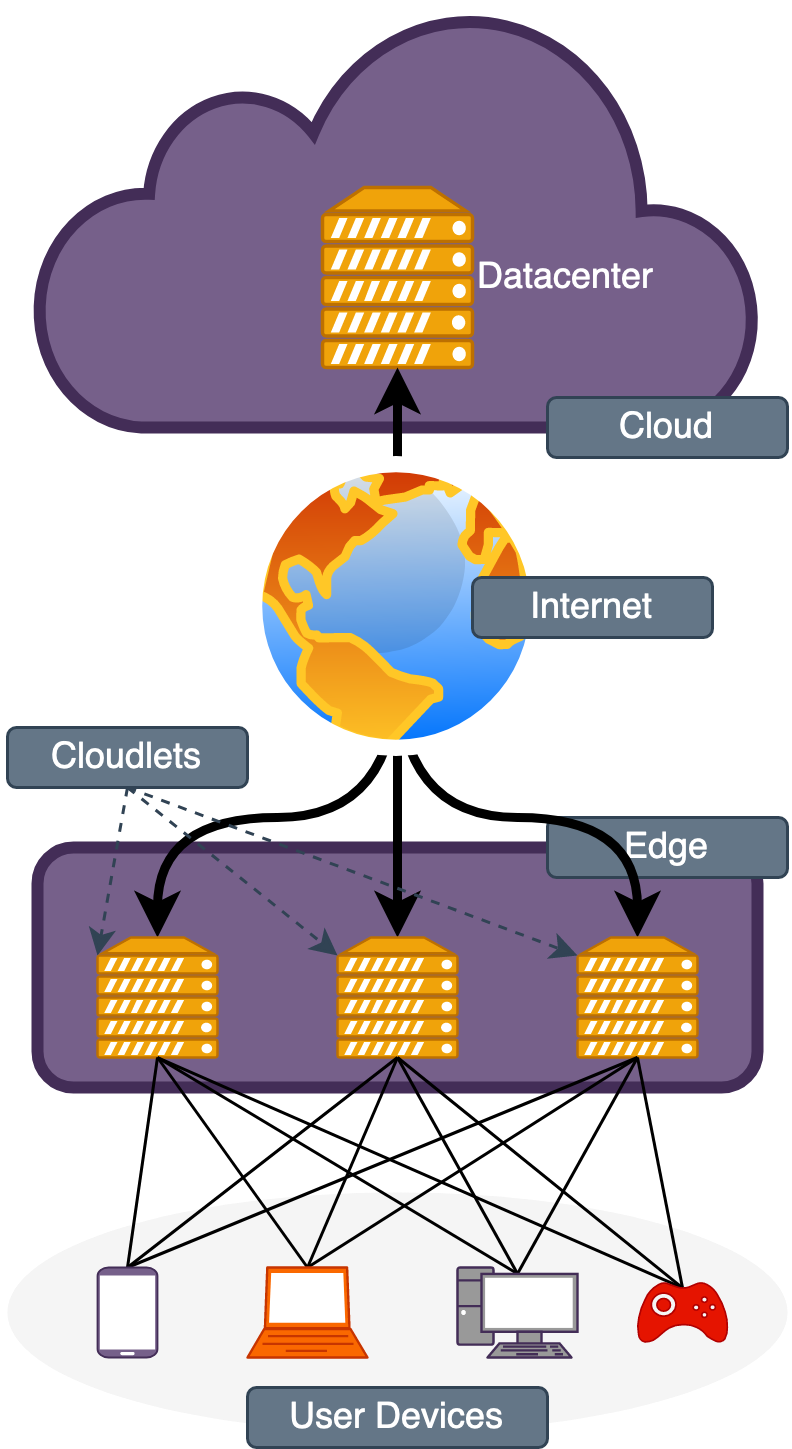
\includegraphics[height=30em]{Figs/edgecomputing}
    \caption{%
        Conceptual design of edge computing.
        Micro-clouds (known as ``cloudlets''~\cite{satyanarayanan2009case}) are placed a at the edge of the network, a few hops away from end users.
        In other words, these cloudlets are located between users and the internet and the cloud.
    }\label{fig:edgecomputing}
\end{figure}

Edge computing, emerges as a potential answer to these challenges~\cite{satyanarayanan2009case,shi2016promise,shi2016edge,varghese2016challenges,satyanarayanan2017emergence,bittmann2017edge,wang2019towards}.
This term refers to a novel distributed computing paradigm, complementary to cloud computing, which tackles the challenges of the cloud by moving computation closer to where it is needed.
Instead of offloading computation to a datacenter potentially thousands of kilometers away, in edge computing it is offloaded to a micro-datacenter --- a \emph{cloudlet}~\cite{satyanarayanan2009case} --- at the \emph{edge} of the network.
These coudlets feature most of the key characteristics of cloud datacenters, such as multi-tenancy, virtualization of computing resources, virtually unrestricted access to energy, as well as limited scalability, one or two hops away from the user (see \cref{fig:edgecomputing})

The architecture of edge computing offers several advantages.
Thanks to their proximity to users, cloudlets can serve highly latency-sensitive and resource-intensive applications with extremely low latencies while still providing orders of magnitude more computing and energy resources than those present on mobile and wearable devices.
Mobile \gls{XR}, such as \gls{WCA}~\cite{ha2014towards,chen2018application,wang2020scaling,chen2017empirical,chen2018application}, and 5G-enabled \glspl{CPS} and \glspl{NCS}~\cite{sasaki2016vehicle,wang2018bandwidth,wan2020efficient} are uniquely poised to take advantage of these characteristic of edge computing.
By processing and aggregating data closer to where its needed, cloudlets can also drastically reduce the amount of traffic going to cloud datacenters.
Cloudlets also present opportunities for increased data security, privacy, and integrity, by keeping it geographically close to its origin and by allowing for anonymization through denaturing and local aggregation before offloading to cloud services~\cite{satyanarayanan2017emergence}.

\todo[inline]{Transition to talk about research and tools for Edge computing research.}

\subsection{\acl{WCA}}
\glsreset{WCA}

There is increasing interest from academia and industry in a novel category of wearable and mobile immersive applications called \gls{WCA}~\cite{ha2014towards,chen2018application,chen2015early,belletier2021wearable,chen2017empirical,wang2020scaling,chatzopoulos2017hyperion}
They represent a particular class of \gls{AR} applications, aiming to amplify human cognition in both day-to-day tasks and professional settings.
\glspl{WCA} operate in a mode analogous to how \gls{GPS} navigation systems guide drivers, by seamlessly providing relevant instructions and feedback relating to the current task at hand and staying out of the way of the user when guidance is not required.
These systems were originally inspired by assistive use cases for people suffering from some form of cognitive decline due to aging, illness, or traumatic brain injury~\cite{ha2014towards,satyanarayanan2019augmenting}.
More recently, their scope has been expanded to include a broader range of use cases, including complex assembly tasks~\cite{chen2017empirical,chen2018application,wang2020scaling,wang2019towards,ha2014towards}.
Non-wearable cognitive assistance systems for assembly tasks have already been proven to be valuable tools in the industrial workplace~\cite{funk2015cognitive,gorecky2011cognito}, and it is understood that the detethering of these system for their use in wearable scenarios opens up a multitude of possibilities.
\todo[inline]{Develop a bit further. Talk about more reactive setups like ping pong too.}

\begin{figure}
    \centering
    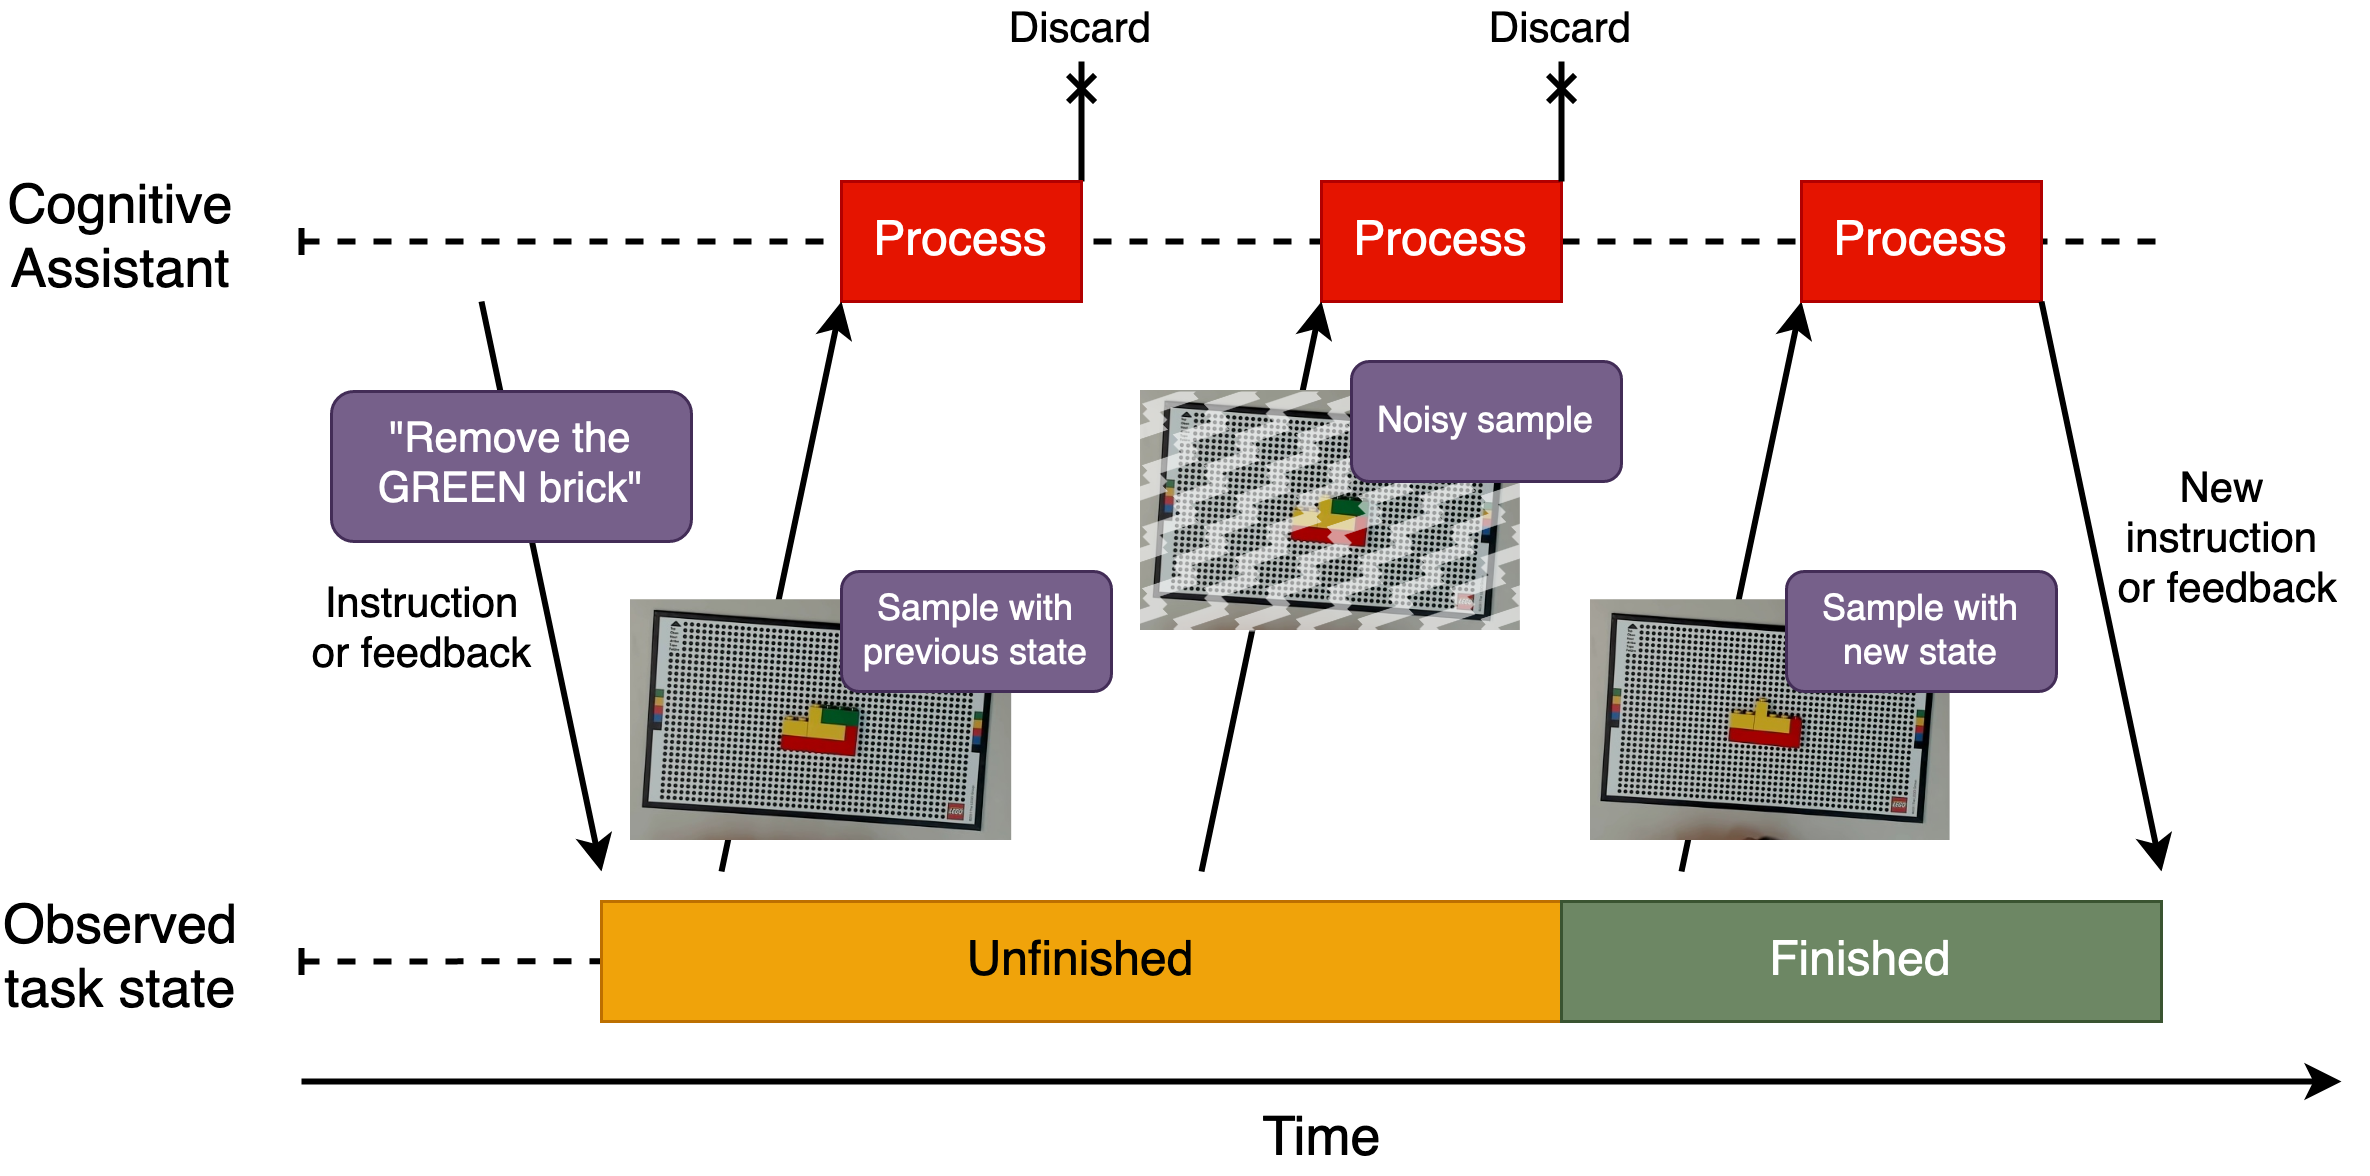
\includegraphics[width=.9\textwidth]{Figs/wca_state}
    \caption{%
        Mode of operation of \gls{WCA} applications.
        The assistant continuously samples the state of the monitored task, and provides appropriate feedback once a state change has been detected.
        Samples that do not result in feedback are silently discarded.
    }\label{fig:wca}
\end{figure}

We identify a number of defining characteristics of \gls{WCA}.
One, and as the name implies, \glspl{WCA} are available whenever the user requires them, without being tethered to a particular physical location;
they are pervasive and mobile~\cite{ha2014towards}.

Next, interaction with \glspl{WCA} is immersive and seamless.
As mentioned above, \glspl{WCA} operate in a manner similar to \gls{GPS} guidance systems.
Through the use of sensors (most commonly video inputs), the application follows the progress of the task in realtime by continuously sampling the state of the physical system.
The input is then parsed to an internal symbolic representation of the state of the task, and whenever a change of state is detected the application provides appropriate feedback or instructions to the user.
Feedback can be in the form of text, images, video, and/or audio, and guides the user towards the next desired system state.
If no change in state is detected, the application remains silent and out-of-the-way of the user;
in other words, samples which capture an intermediate or unfinished state, or simply noise are silently discarded.
\Cref{fig:wca} illustrates this mode of operation in a \gls{WCA} guiding a user to manipulate a structure composed of LEGO bricks.
Assistants should be able to analyze the current context and automatically provide relevant feedback without explicit commands from the user.
\gls{WCA} is expected to operate much like a human assistant would, by observing the performance of the user and offering guidance proactively.

Note that this mode interaction implies seamless integration of the application with the context of the user and the real world.
The user does not trigger an update explicitly at any point, leading to one of the key characteristics of \gls{WCA}.
The only points in time at which a user can consciously notice and interact with the application is whenever they are \emph{expecting} feedback.
An important corollary of this is that these are therefore the \emph{only} points in time at which users can notice changes in system responsiveness.

Finally, feedback in \gls{WCA} systems should be provided ``quickly'' (relative to the task at hand) to the user.
This goes hand in hand with the previous characteristic of seamless interaction, as users will have expectations of constant and immediate feedback as they interact with the system.
As is the case for most \gls{XR} applications, delayed feedback in \gls{WCA} can have severe negative consequences for the quality of the user experience.
Depending on the task, these consequences can range from simply distracting or annoying the user (in the case of less interactive tasks such as step-by-step assembly), to actively handicapping user performance (in the case of highly interactive tasks).

The above characteristics together lead to interesting consequences for \gls{WCA} system design.
Their wearable nature directly implies use of lightweight and battery-powered devices, greatly constrained in terms of energy and computing resources.
The requirement of immersive and seamless interaction suggests a level of context sensitivity and proactivity that can only be provided by real-time analysis of sensor inputs such as video and audio feeds.
This kind of compute- and energy-intensive processing is unfeasible to be performed on wearable devices, and thus these applications necessarily make use of compute offloading.
As explained above, the cloud is unsuitable as an offloading point for these applications, given the high latencies incurred, and there is thus a broad understanding today that with the advent of edge computing, \glspl{WCA} will become a practical reality~\cite{bittmann2017edge,flinn2012cyber,chen2017empirical,ha2013just,wang2020scaling,chen2018application,ha2014towards}.

There's more to end-to-end latency than merely the question of where the compute backend is placed, however.
The design of any complex application such as \gls{WCA} involves a multitude of decisions with the potential to influence the system responsiveness as experienced by the user.
These decisions include those on the implementation side (compression standards, algorithms, protocols, etc.), as well as on the infrastructure side (physical network layer, traffic prioritization, etc.).
Existing studies of this class of applications have only recently started to delve more deeply upon these issues~\cite{chen2017empirical,wang2019towards,wang2020scaling,ha2014towards,chen2015early,satyanarayanan2009case,chatzopoulos2017hyperion}.
Recently published models for end-to-end latency of edge computing architectures, on the other hand, are quite complex, while not accounting for the specifics of human-in-the-loop applications and in many cases limited to very constrained scenarios and analyses~\cite{al_zubaidy2015performance,schiessl2017finite,moothedath2022energy2,moothedath2022energy1,moothedath2021energy}.
\todo[inline]{%
    Maybe also present ``other'' research on WCA here? E.g.\ other research in WCA has focused on... So-and-so have... blah blah.
}
The present thesis aims to contribute to this body of work by presenting and discussing a viable methodology for the design and evaluation of these systems.

\subsubsection{Characterization of \acs{WCA}}

\begin{figure}
    \centering
    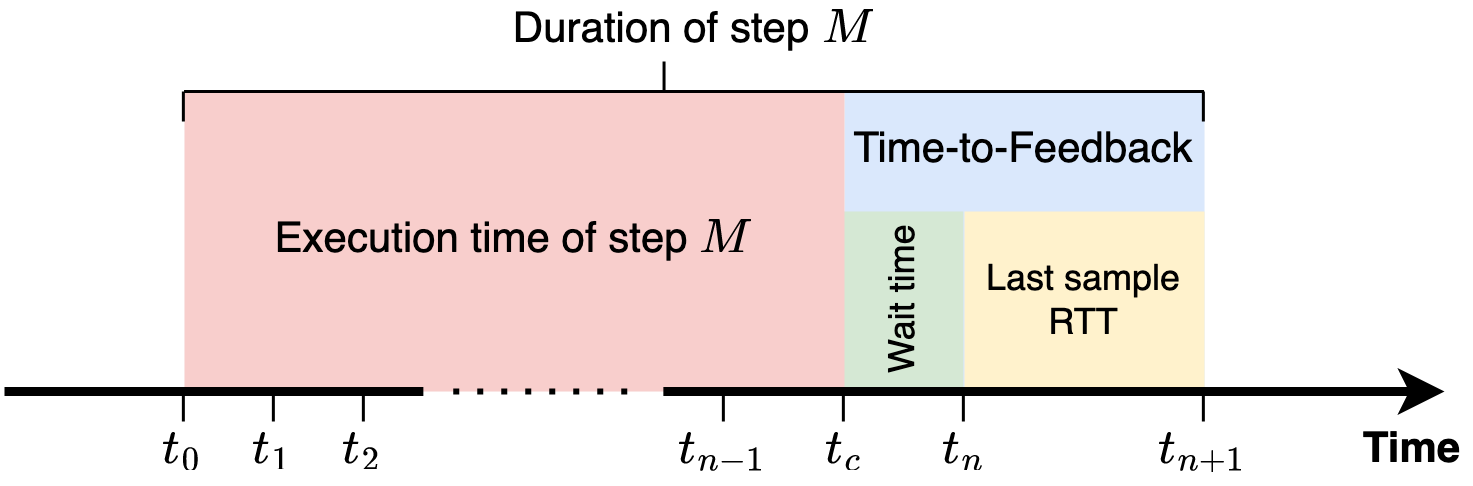
\includegraphics[width=.9\textwidth]{publications/2023EdgeDroid2/figs/step_time}
    \caption[]{%
        Breakdown of a step in a \gls{WCA} into its timing components.
        \ensuremath{t_k | k \in \{1, \ldots, n \}} correspond to sampling instants.
        \ensuremath{t_0} indicates the instant at which the instruction for step \ensuremath{M} is provided to the user and the first sample for said step is captured.
        The instruction for step \ensuremath{M + 1} is provided at \ensuremath{t_{n+1}}.
        Finally, \ensuremath{t_c} marks the instant at which the user finishes the instruction, and \ensuremath{t_n} the instant of capture of the first sample after the instruction has been completed;
        this sample therefore also corresponds to the final sample of step \ensuremath{M}.
        Figure originally included in \cref{paper:olguinmunoz2023realistic}.
    }\label{fig:wcastep}
\end{figure}

An important portion of the present thesis deals with the modeling of human behavior for the benchmarking of \gls{WCA}.
We focus in particular on \emph{step-based} \gls{WCA}, i.e.\ assistance applications which have as their goal the guidance of a user through a task, using a series of instructions.
In this section, we will provide some definitions relating to the operation of these applications.

As discussed above, \glspl{WCA} track the state of the real world through sampling of inputs, most commonly of video feeds.
In step-based \glspl{WCA}, the state in question refers to the progress of some arbitrary, sequential task, such as the assembly of a LEGO model or of a piece of IKEA furniture~\cite{chen2018application}.
We will formally define \emph{task} as a well-defined sequence of instructions to be performed in order to achieve a final goal state, and further define a \emph{step} within a task as a specific action to be performed by the user, described by a single instruction.
A step begins when the corresponding instruction is provided to the user, and ends when the instruction for the next step is provided;
the time interval between these two events will be referred to as the \emph{step duration}.

In the following, please refer to \cref{fig:wcastep}.
\ensuremath{\{ t_0, t_1, \ldots, t_{n + 1} \}} corresponds to a series of discrete and sequential sampling instants, such that \ensuremath{t_0} corresponds to the instant at which the instruction for step \ensuremath{M} is provided and the first sample of the step is taken.
\ensuremath{t_n} corresponds to the instant at which the final sample of step \ensuremath{M} is taken;
this sample is the first sample to capture the finished state of the step.
At this point, the application transitions to the next step \ensuremath{M + 1}, and thus \ensuremath{t_{n + 1}} is the instant at which the next instruction is provided and step \ensuremath{M + 1} begins.
We will also refer to the interval \ensuremath{t_{n + 1} - t_n} as the \emph{last sample \gls{RTT}}.

\glsreset{TTF}%
From this characterization, we can define key variables relating to human behavior with respect to the sampling behavior of these applications.
If we understand \ensuremath{t_c} as the point in time at which the user finishes executing the instruction for step \ensuremath{M}, then
\begin{inlineenum}
    \item \ensuremath{t_c - t_0} corresponds to the \emph{step execution time}, that is, the time it has taken the user to complete the instruction
    \item \ensuremath{t_n - t_c} is the \emph{wait time}, an interval of time during which the task has been finished, but no sample capturing the new state has been taken yet
    \item finally, the interval \ensuremath{t_{n + 1} - t_c} we call \emph{\gls{TTF}}, and refers to the time the user spends waiting for a new instruction.
\end{inlineenum}
These values are key to understanding human perception of responsiveness in these systems, and therefore also to the optimization of resource consumption in \gls{WCA}.
We will refer to them extensively in \cref{chap:contributions}.

%\subsection{Mechanisms relating human behavior to system responsiveness}
%
%The question of how people respond to delay in a computer system is grounded in how people perceive time.
%Time perception has been described as regulated by an attentional gate that, when opened, starts a cognitive pulse counter~\cite{zakay1995attentional,zakay1996role}.
%More recent research indicates, however, that duration perception is highly malleable and the result of multiple timing mechanisms found in overlapping, flexible neural systems~\cite{bruno2016multiple,wiener2011multiple}.
%The estimation of an event's duration varies with context of various types
%\begin{inlineenum}[label={(\roman*)}, before=\unskip{: }, itemjoin={{; }}, itemjoin*={{; and }}]
%\item events subsequent to a long or short interval are contracted or extended, respectively~\cite{heron2012duration}
%\item repeated events tend to be perceived as shorter than novel ones~\cite{matthews2011stimulus}
%\item arousal can expand durations~\cite{droit_volet2011emotion}.
%\end{inlineenum}
%
%Expectations play a critical role in time perception as well~\cite{zakay1995attentional,zakay1996role}.
%It has been shown that people have a general tendency to be hypersensitive to delays in worse-than-expected states, and under-sensitive to meeting or exceeding expectations~\cite{loewenstein1992anomalies}.
%Accordingly, failures to meet expected fast response times tend to be experienced as highly negative, whereas fast latencies are not noticed.
%Violations of expectancy have a strong impact on the acceptability of computer systems.
%Users of a computer system anticipate the latency for events, for which the standards only become more stringent as systems improve in response time.
%In immersive systems like \gls{WCA}, which aim to provide seamless interaction, delays are particularly noticeable.
%
%It has long been recognized that slow system response times can undermine cognitive processing, slow the pace of users, and lead to stereotyped behavior and errors, as well as cause negative emotional consequences~\cite{dabrowski201140}.
%However, standards for what constitute tolerable delays have changed dramatically compared to three decades ago, when delays on the order of \SI{10}{\second} were deemed acceptable~\cite{nielsen1994usability, shneiderman2016designing, seow2008designing}.
%Today's user context, and \gls{WCA} in particular, often demand response times orders of magnitude shorter.
%
%For \gls{WCA} the acceptable range for latencies was explored by Chen et al.~\cite{chen2017empirical}, by constructing assistants for tasks with a range of time constraints, including step-by-step tasks and more interactive contexts like playing Ping-Pong against a human opponent.
%They then proposed a latency tolerance zone according to the task demands.
%For an essentially self-paced task like LEGO assembly, they found two key ranges of latency; unnoticeable, \SIrange{0}{0.6}{\second}; and impaired, \SIrange{0.6}{2.7}{\second}.
%Beyond that, users could begin to show the negative outcomes previously catalogued~\cite{dabrowski201140}.
%
%While behavioral changes and negative interaction outcomes have been well documented in prior research on system delay, the specific mechanisms that mediate these outcomes are less well understood.
%These mechanisms could be cognitive or emotional in origin.
%
%A first possible explanation comes from research on cognitive and motor planning.
%Delay may move users from relatively automatic to more attention-demanding processing.
%Cognitive and motor tasks are commonly described as a hierarchical system, progressing from high-level goals to the sequence of commands that accomplishes them.
%As competency in a task increases, execution of the hierarchy becomes increasingly automated.
%Automatization has been described from a computational perspective in {Anderson's ACT-R}~model as the compiling of multiple productions into one~\cite{neves1981knowledge}.
%Neural measurements indicate that with automaticity, control moves from frontal brain areas to more posterior ones~\cite{jeon2015degree,puttemans2005changes}, and similar distinctions have been related to temporal processing~\cite{lewis2003distinct,koch2009neural,lee2019limiting}.
%
%Although activities guided by a \gls{WCA} are not simple motor actions, immediate feedback after each of a series of repeated actions should promote development and automatic execution of a hierarchical plan.
%Delays, in contrast, would disrupt such a plan through the loss of automated control~\cite{lee2019limiting}.
%
%A second, alternative explanation of delay effects appeals to emotional systems rather than cognitive processes.
%As users of a system become emotionally aroused by delay, they may be subject to generalized arousal, causing decrements in performance~\cite{lee2019limiting}.
%
%Finally, a third potential explanation of delay effects is what has been called ``ego depletion'', the notion that expending effort on self-control eliminates resources needed for further effort~\cite{baumeister74tice,lin2020strong}.
%
%The various processing accounts of delay effects predict different outcomes, which we will consider in the context of the current data.
%If delay increases attentional demands on cognitive processes, responses should be slowed and errors expected, particularly on time-critical tasks.
%Generalized arousal triggered by emotional stress from delay should emerge in physiological measures, such as increased heart rate or skin conductivity.
%Arousal can also reduce movement smoothness or add erratic gestures~\cite{pijpers2003anxiety}.
%Ego depletion has been found to produce premature responses culminating in error~\cite{lin2020strong}, or to lead to abandoning a task entirely~\cite{baumeister74tice}.
%
%Over-arching prescriptions for tolerable system response time have not tended to take into account individual differences in users with respect to salient variables like cognitive ability or personality.
%Relevant research can be found in studies of delay discounting, the tendency to devalue rewards for which one must wait.
%High discounting rates, indicative of waiting intolerance, have been associated with negative social and academic outcomes.
%Hirsh et al.~\cite{hirsh2008delay} found that higher discounting was associated with extraversion among those with low cognitive function, whereas lower discounting was associated with emotional stability (low neuroticism) for people with high cognitive function.
%Among computer system users who tend to have relatively high cognitive ability (which presumably describes the present experimental population), this points to neuroticism as a personality factor that might modulate tolerance for waiting. Extraversion could also  be  a moderating factor among the broader target audience of \gls{WCA}, which are intended for relatively inexperienced users of an application.
%These and other measures of individual variation were considered here.

\subsection{\acsp{NCS} and other \acsp{CPS}}

The number and applications of \glspl{CPS}~\cite{Rajkumar2010CPS} --- i.e.\ systems in which a real, physical mechanism is controlled by a computer --- have exploded in recent years.
However, this rapid increase in adoption has mostly been limited to industrial contexts.
Although \glspl{CPS} present huge opportunities for all facets of society, they have yet to reach our daily lives in any relevant scale due to their stringent operational requirements.
This is about to change, however, as with the advent of novel wireless communication technologies as well as networking paradigms, such as cellular 5G and edge computing~\cite{Satya2017Emergence}, consumer-grade \glspl{CPS} will be made possible.
These technologies meet two key requirements of \glspl{CPS}: real-time capabilities (through extremely low end-to-end latencies), and context- and locality-awareness, and will most likely become the backbone of \gls{CPS} in the future.

\glspl{NCS}~\cite{Gupta2010NCSOverview}, a type of \gls{CPS} wherein multiple networked actuators and sensors form a part of the same automatic control system will benefit from the adoption of these technologies.
Depending on the physical system being controlled, \glspl{NCS} can have stringent timing and reliability requirements for communication that conventional cloud paradigms and cellular networks cannot meet~\cite{Wan2020Efficient}.
This necessitates sophisticated tools for the performance evaluation of future system architectures, as well as novel NCS design paradigm.

%Due to their potential advantages for industrial and commercial settings, there exist works~\cite{Zhang2016Survey} dedicated to the modelling and performance characterization of \glspl{NCS}, improving NCSs by distributing control functions across networks, facilitating centralized coordination, control, and monitoring.

One the one hand, related literature in \glspl{NCS} leverages to a large extent theoretical models, at the price of being able to capture networked systems effects only on a coarse level.
%follows a theoretical approach, and only a small fraction of it deals with experimental studies.
On the other, there exist several approaches when considering experimental methodologies.
%A number of works concerning \glspl{NCS} deal with experimental studies.
%\glspl{NCS} have an inherently inter-domain nature intertwining knowledge from the fields of communications, computing, and control theory in ways that cannot be studied in isolation, leading to various different approaches to such studies.
One such approach uses setups in which the complete system is built on top of real hardware.
This approach is employed in the works of Baumann \emph{et al.}~\cite{Baumann2018LowPower} and Cuenca \emph{et al.}~\cite{Cuenca2019UAV}; in both of these, the authors implement their approach on physical testbeds.
Conversely, other studies choose to instead use completely \emph{simulated} \gls{NCS} setups.
The authors in\ \cite{Ma2019DynamicSched} have opted for such an approach.
These studies often employ combinations of physical and network simulation tools trying to capture the complex dynamics of \glspl{NCS}.
Finally, some experimental studies instead employ \emph{virtualized} approaches, in which either
\begin{inlineenum}[itemjoin={{; }}, itemjoin*={{; or }}]
    \item a real network interacts with a simulated or emulated control system~\cite{Wang2020VoltageControl}
    \item a simulated network interacts with a real control system~\cite{Natale2004InvPendEthernet}.
\end{inlineenum}

As evidenced above, experimental research in \glspl{NCS} includes varied heterogeneous hardware and software platforms, methodologies and key performance indicators.
This, in turn, leads to hardware, software, and methodology fragmentation, as different studies tend to prefer approaches more favored in their respective communities.
Furthermore, existing studies tend to focus on individual aspects and components of a system, thus producing results which do not provide a complete image of the \gls{NCS}.
This has caused a gap in knowledge pertaining to the reproducibility and comparison of experimental studies on these systems.

Zoppi \emph{et al.}~\cite{Zoppi2020NCSBench} made the first (and to the best of our knowledge, the only) attempt at tackling this challenge in their work.
In their work, they proposed a platform called NCSBench, to be used for reproducible benchmarking in NCS.\
Their methodology utilizes joint knowledge of control, computation, and communication.
In their work various architectural elements and the corresponding delays associated with the NCS are modelled.
Multiple experimental parameters and certain observable key performance indicators are defined and utilized in the implementation.
This work however utilizes a physical LEGO\textregistered{}\ Mindstorms EV3 Core Set\texttrademark{}\  based plant for the implementation, preventing instantaneous changes in plant characteristics and component parametrizations.
Furthermore, relying on physical objects like an inverted pendulum limits scalability of the experimentation in practice.

\subsubsection{Benchmarking tools for edge computing}

Experimental research in the area of wireless networking has received ever increasing attention over the last years, driven, on the one hand, by the complexity of modern networked systems and corresponding applications.
On the other, networked systems are more and more based on software instead of dedicated hardware, which allows experimental testbeds to be rededicated simply through an update as system versions evolve --- in contrast to the redeployment of hardware necessitated \numrange[range-phrase={--}]{10}{15} years ago.
The complexity of these systems, as well as their softwarization are expected to continue growing, driving in turn an expanding interest in testbed-based experimental research in wireless systems.

Over the last years, several small- to mid-scale testbeds have emerged that leverage a large degree of freedom with respect to hardware and software, for example, the
\begin{inlineenum}
    \item \gls{COSMOS}
    \item \gls{POWDER}
    \item \gls{ARA}
    \item Drexel Grid \gls{SDR}
\end{inlineenum} testbeds.
\gls{COSMOS} is a testbed spanning an area of roughly \num{1} square mile (\SI{2.6}{\kilo\meter\squared}) featuring \glspl{SDR}, \si{\milli\meter}-wave equipment, optical fibers, cloud integration, and compute for core network functionality and application data processing~\cite{Cosmos1,cosmos2}.
It contains over \num{200} rooftop, intermediate, and mobile nodes, and is controlled and managed by a central node.
\gls{COSMOS} relies on the \gls{OMF} (originally developed for ORBIT~\cite{orbit}), and employs the \gls{OEDL}, a domain-specific imperative language based on Ruby, for experiment development and definition.

\gls{POWDER} promises research on wireless and mobile networks with a level of programmability down to the waveform~\cite{powder}.
The testbed spans a \SI{15}{\kilo\meter\squared} area and features about \num{15} fixed programmable radio nodes, based on off-the-shelves \glspl{SDR} and featuring edge-like compute capabilities and integration with cloud resources, which interact with \num{50} mobile nodes.
\gls{POWDER} experiments are defined and developed in \emph{profiles}, which correspond to \gls{VM} images containing the necessary software and configurations.
These profiles are defined through using \gls{RSpec}\footnote{\url{https://groups.geni.net/geni/wiki/GENIExperimenter/RSpecs}} documents.

The \gls{ARA} platform is an at-scale testbed for wireless research spanning a rural area with a diameter of over \SI{60}{\kilo\meter} in Iowa~\cite{zhang2022ara}.
Its core goal is the study and deployment of advanced wireless platforms and technologies in real-world agricultural and rural settings.
It includes a broad range of wireless platforms ranging from low-\gls{UHF} massive \gls{MIMO} to \unit{\milli\meter}Wave, deployed through both \glspl{SDR} and programmable \gls{COTS} radios, as well as automated ground vehicles, cameras and sensors.
\gls{ARA}'s software stack, ARASoft, is based upon the highly flexible and powerful \gls{CHI} software suite from the Chameleon testbed project~\cite{keahey2020lessons}, which in turn is based on the widely adopted OpenStack~\cite{openstack} cloud-computing framework.
This affords the \gls{ARA} testbed a high degree of flexibility, as well as lowers the learning curve for new contributors and users.

Finally, the \emph{Drexel Grid \gls{SDR} Testbed} features \glspl{SDR} that connect either over-the-air, through a channel emulator, or over a combination of the two, to facilitate realistic and reproducible experimentation~\cite{DrexelGrid}.
Primarily intended for \gls{SDR}-centric research, it does not integrate any core, cloud or edge components.
However, the testbed extensively employs the \gls{LXC} runtime for the deployment of both experimental code and \gls{SDR} software, which affords users great freedom when it comes to the development of experiments.

Experimentation is key to to fully understanding the implications of next-generation wireless systems, cloud, and edge computing paradigms, and thus more of these testbeds are sure to emerge in the near future.
Yet, little work has so far been devoted to general-purpose, hardware-agnostic software frameworks for the management and automation of such systems.
Existing platforms implement their own, ad-hoc software solutions which are not compatible with other testbeds, and in many cases are not even compatible with reigning cloud-native standards.
This is, for instance, the case with \gls{COSMOS} and \gls{POWDER}; their reliance on domain-specific languages limits their integration with cloud-native solutions, which generally build upon general-purpose languages such as Python and Go.
These testbeds further leverage virtualization technology based on \glspl{VM} instead of more lightweight and edge-compatible solutions such as containers.

To the best of our knowledge, CloudRAFT~\cite{cloudraft} is the only work to tackle (to a certain extent) this challenge.
CloudRAFT corresponds to a cloud-based framework for mobile network experimentation, with a focus on simplifying the management of testbed resources.
The goal of this project is to integrate, coordinate, share, and improve upon existing testbeds; and employs pre-built \glspl{VM} containing the necessary software for experiments.
Although it provides some automation for testbed resource provisioning and experiment execution, its focus is largely rather on the sharing and partitioning of testbed systems.
Testbeds currently working with CloudRAFT include a variety of domain-specific setups, including \pgls{SDR}-based testbed as a well as a ground vehicular robot for mobility-related experimentation.


\chapter{Key Contributions \& Results}\label{chap:contributions}
\chapter{Key contributions and results}\label{chap:contributions}

\section{A methodology for the study of feedback-loop systems in Edge Computing}\label{summary:methodology}

\begin{figure}
    \centering
    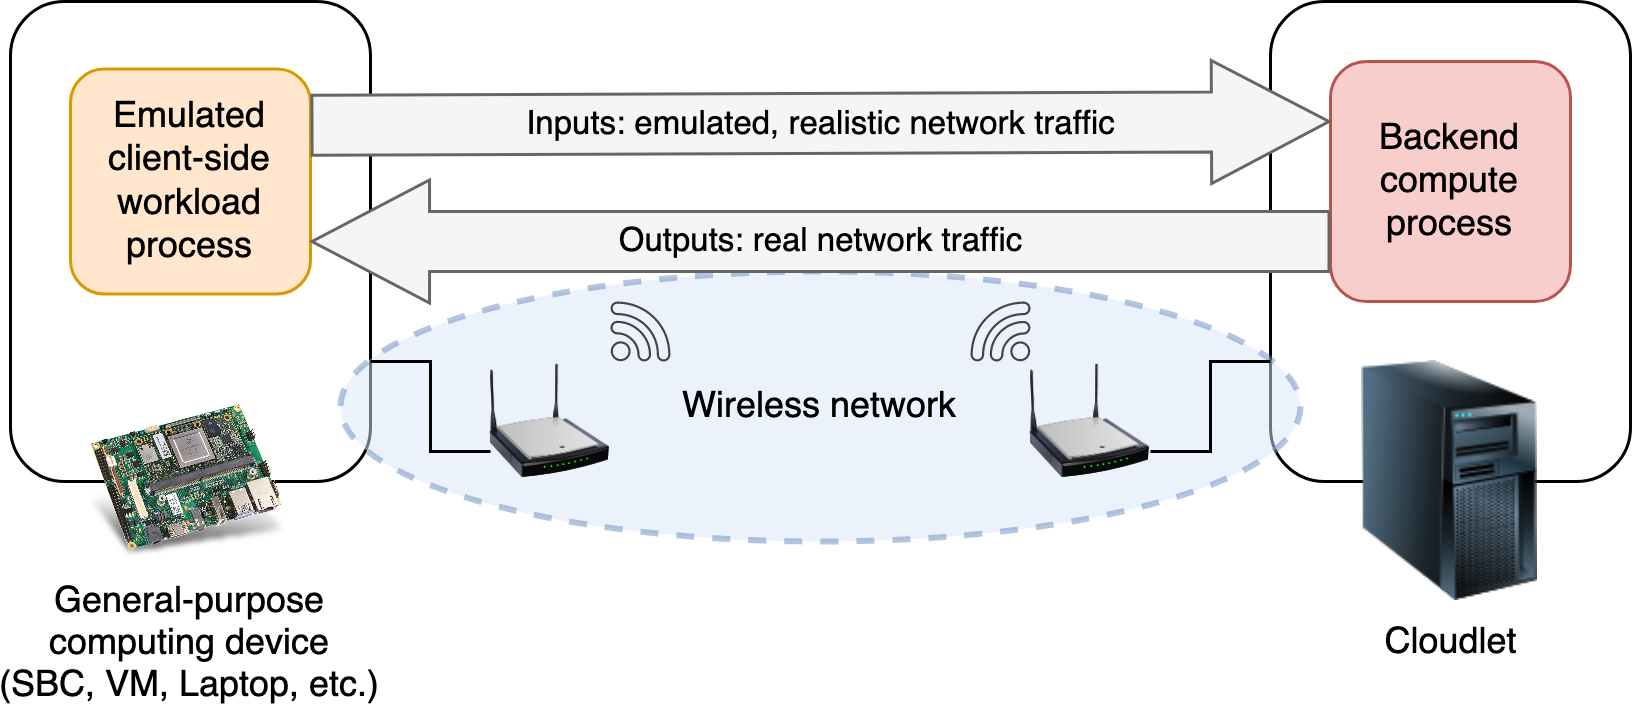
\includegraphics[width=.8\textwidth]{Figs/methodology.png}
    \caption{%
        Overview of the proposed methodology for the study of feedback-loop systems on edge computing infrastructure.
        The  client side of the system is replaced with an emulation executed on a general-purpose computing device.
        The backend/server side of the system along with the network remain unchanged.
    }\label{fig:methodology}
\end{figure}

As discussed above, benchmarking infrastructures for edge-bound applications featuring feedback-loops is challenging, in particular when dealing with applications with high sensitivity to latency (such as \ac{NCS}) or with human involvement (such as \ac{WCA}).
In the following, we introduce our methodological framework for tackling this challenge.

A general overview of our methodology is illustrated in \cref{fig:methodology}.
It is based on the core idea of executing an emulation of the target workload on top of the real hardware on which it is to be deployed.
We replace the client side of the system with a realistic emulation of the desired behaviors; this emulation is implemented in software deployed on \ac{COTS} general-purpose computing devices.
The backend side and the network are not changed.

Two main arguments drive this approach.
One, the difficulty of scaling the number of clients in these systems in a research context.
The systems we target exhibit a centralized nature in which a potentially large number of clients offload computation to a single central compute node.
The client-side component of the applications of interest for this research is often complex to scale, either due to the involvement of humans (as in the case of \ac{WCA}) or due its cyber-physical nature (in \acp{NCS}).
Emulating this component reduces this complexity by moving it into the software domain, allowing for easier scaling through the use of cheap, general-purpose hardware such as single-board computers (e.g. Raspberry Pis, Beaglebones, etc.).

And two, it maintains the realism of the most complex parts of the system.

\todo[inline]{Fix and finish}

In the following, we will discuss the initial implementation of this methodology to two different classes of applications.
We first discuss the methodology in the context of a human-in-the-loop application, \acl{WCA}, in section \cref{ssec:methodology:wca}.
Then, in \cref{ssec:methodology:ncs}, we present an exploration into it's utility for the study of \acf{NCS}.


\subsection{Applying the methodology to \acs{WCA}}\label{ssec:methodology:wca}

\begin{figure}
    \centering
    \begin{subfigure}[b]{.47\textwidth}
        \centering
        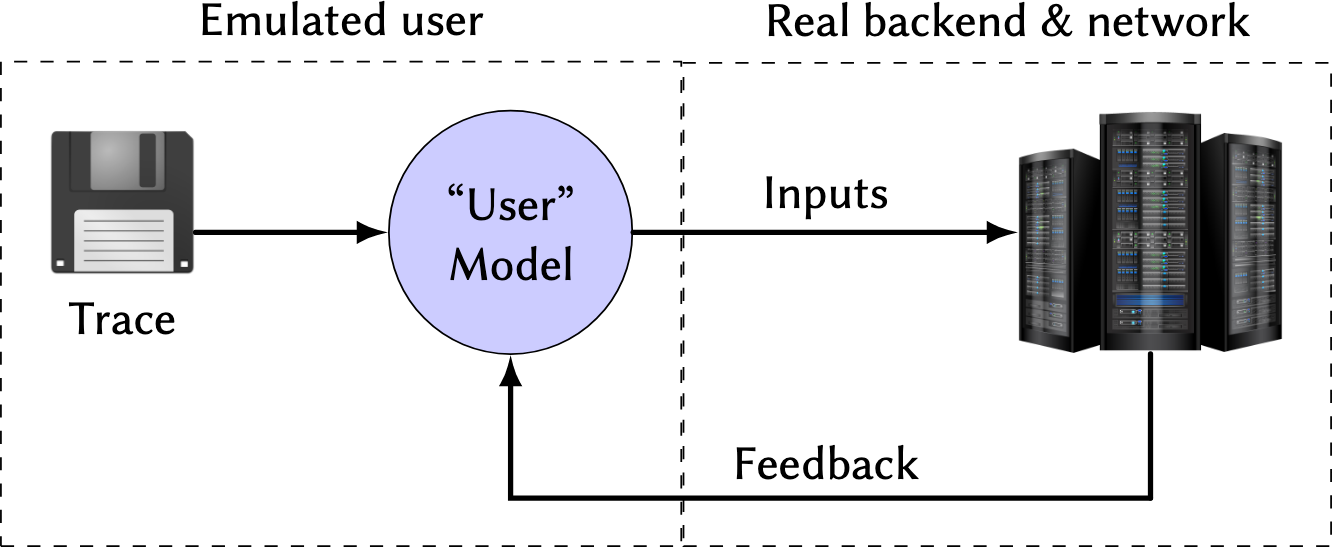
\includegraphics[width=\textwidth]{Figs/trace_edgedroid.png}
        \caption{%
            High level conceptual design of our methodology for \ac{WCA}.
            We replace the human by a trace-driven emulation.
            This allows us to maintain realism in inputs sent over the network to the compute process on the backend, while simplifying the design of the client software.
        }
    \end{subfigure}
    \hfill
    \begin{subfigure}[b]{.47\textwidth}
        \centering
        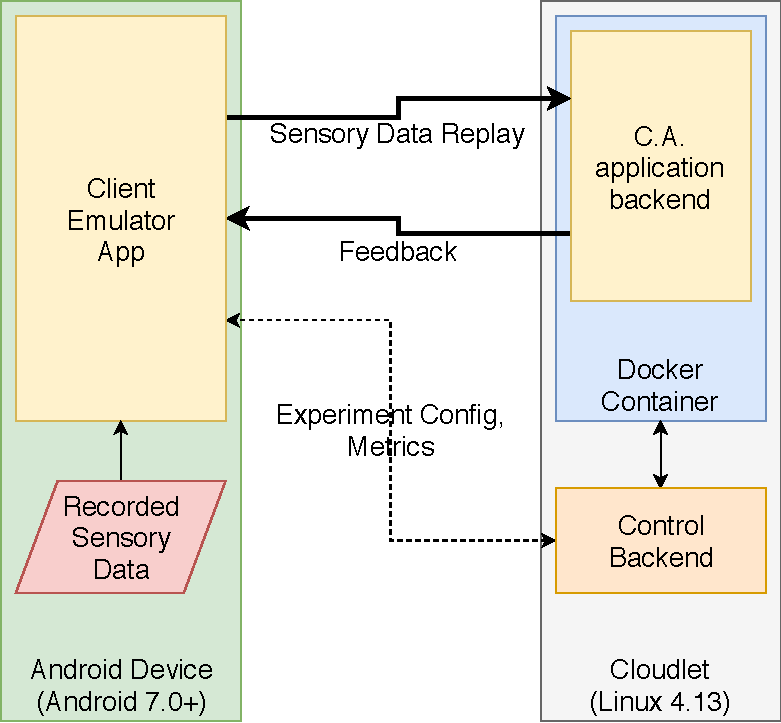
\includegraphics[width=\textwidth]{publications/2018DemoScalingOnTheEdge/img/TraceReplay_GenArch}
        \caption{%
            Architectural overview of the EdgeDroid \num{1.0} tool.
            The ``client emulator app'' implements the aforementioned user model together with the required networking functionality to connect to a \ac{WCA} backend running on a cloudlet.%
            }
    \end{subfigure}\\
    \medskip
    \begin{subfigure}[t]{\textwidth}
        \centering
        \adjustbox{scale=0.7}{
            \begin{tikzpicture}[align=center,
            node distance=.5cm and 1.5cm,
            every initial by arrow/.style={-{Latex[length=2mm]}}]
            % Place nodes              
            \node [initial, state, minimum size=6em, initial text=] (play) {Play};               
            \node [state, above right=of play, minimum size=6em] (change) {Change\\step};
            \node [state, below right=of play, minimum size=6em] (rewind) {Rewind};
            \node [state, accepting, above right=of rewind, minimum size=6em] (shutdown) {Shutdown};
            
            % Draw edges
            \path[draw, -{Latex[length=2mm]}]
            (play) edge [bend right=20] node[left] {Step done} (rewind)
            edge [bend left=20] node[left] {Got feedback\\(\emph{positive})} (change)
            edge [out=140,in=220,looseness=6] node[left] {Step\\not done} (play)
            
            (change) edge [bend left=20] node[right] {Step changed} (play)
            edge [bend left=20] node[right] {All steps done} (shutdown)
            
            (rewind) edge [bend right=20] node[right] {Rewound} (play)
            edge [bend right=20] node[right] {Too many rewinds} (shutdown);
            
            \end{tikzpicture}
        }
        \caption{State diagram of the user model governing the replay of the pre-recorded trace at runtime. This model approximates the behavior of an ``ideal'' human, one that is patient and makes no mistakes.}\label{fig:usermodel}
    \end{subfigure}
    \caption{%
        Overview of our first implementation of the methodology for \ac{WCA}.
    }\label{fig:edgedroid1:trace}
\end{figure}

We first introduce our methodology in \cref{paper:olguinmunoz2018demoscaling,paper:olguinmunoz2019edgedroid}.
The former corresponds to an extended abstract paper which discusses a high level overview of our approach; the latter presents a deeper, more complete discussion about the implementation together with some first experimental results.

The overall goal of these papers is to explore this methodological approach as applied to \ac{WCA}.
As discussed in \cref{chap:introduction}, the main challenge to benchmarking \ac{WCA} --- and other ``human-in-the-loop'' applications on the edge --- concerns the involvement of human beings in their operation.
Humans are unreliable, and, perhaps more importantly, hard to scale.
\todo[inline]{More reasons}

The implementation of the client-side emulation necessary for our methodology follows in these works a trace-based design.
We introduce a tool, \emph{EdgeDroid \num{1.0}}, which replays a pre-recorded trace of sensory inputs to the original \ac{WCA} backend.
The tool is implemented in Android, allowing for its easy deployment on the same kind of \ac{COTS} mobile devices on which real \ac{WCA} applications are intended to run in the future.
Furthermore, this tool is instrumented, allowing us to collected a multitude of system-level metrics at runtime which can then be analyzed.
On the other hand, the trace in question corresponds to a pre-recorded sequence of sensory inputs obtained from a real execution of the \ac{WCA} by a human volunteer.
The trace is recorded in a near-ideal setting, such that it does not include either human mistakes or segments with degraded system responsiveness.
Once recorded, the trace is manually segmented into the logical component steps of the task, and these are replayed in sequence back to the backend by the EdgeDroid tool.

We opt for a trace-based approach for our first implementation of the methodology for \ac{WCA} for three key reasons.
The first of these is the level of realism if affords in terms of the payloads sent over the network and, in particular, processed by the backend.
Using a trace ensures that the same computation is performed on the edge as if a human was involved, while also ensuring a reproducible application execution path.

The second is simplicity, as such an approach does not require complex modeling of human behavioral patterns, merely the observation and recording of them.
Compatible traces can be easily obtained simply by instrumenting existing \ac{WCA} client applications to record all captured inputs.

The final advantage corresponds to extensibility.
As long as the tasks belong to the same category of \ac{WCA} applications (in this case, step-based cognitive assistance), using a trace makes extending the tool to different tasks merely a matter of recording a new trace.

\todo[]{}



reproducible and comparable workload, we use a trace-based design for the client-side emulation.
.

To then use the trace for reproducible experiments, we introduce a benchmarking suite which can replay the trace to the original application.
This results in the same computation to be performed on the edge as if a human was involved, while also ensuring a reproducible application execution path.
Additionally, the suite is instrumented to collect system level metrics at runtime for posterior analysis.

However, merely replaying the trace is not enough, as disparities between system responsiveness at recording versus replay time can cause the trace so drift out of synchronization with the current state of the system.
Thus, we introduce here the concept of a human user model which is able to adapt its behavior in a realistic manner based on the current responsiveness of the system by systematically controlling the replay of the trace.
The initial approximation we introduce, illustrated in \cref{fig:usermodel}, here is that of a human that is patient and does not make mistakes, and any error message received from the application backend is ignored.
The trace is preprocessed into segments that correspond to individual steps of the \ac{WCA} application; this is performed manually as a preparation step.
The user model then replays each segment in order; whenever feedback corresponding to a change of step is received from the \ac{WCA} backend, the user model transitions to the next segment in the trace, no matter whether the current segment has been replayed out completely or not.
On the other hand, if no step transition feedback has been received at the end of the current trace segment, the model rewinds the trace a $\tau$ seconds and tries again.
To avoid infinite loops, where the application is stuck on a step forever, we have a maximum number of possible rewinds, after which the application shuts down.

\todo[inline]{EdgeDroid paper}



\begin{figure}
    \centering%
    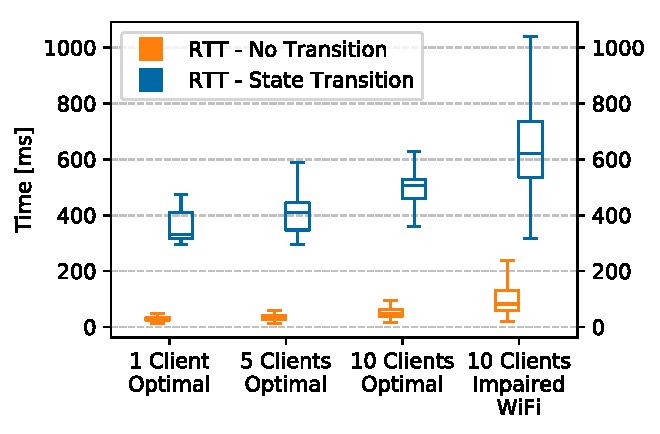
\includegraphics[width=.85\textwidth]{publications/2019EdgeDroid/plots/comparison/nofonts/rtt_fb_vs_nofb}%
    \caption{Comparison of round-trip-times for inputs that triggered a state transition in the task model versus inputs that did not.}%
    \label{fig:comparison:rtt}%
\end{figure}%
\begin{figure}
    \centering%
    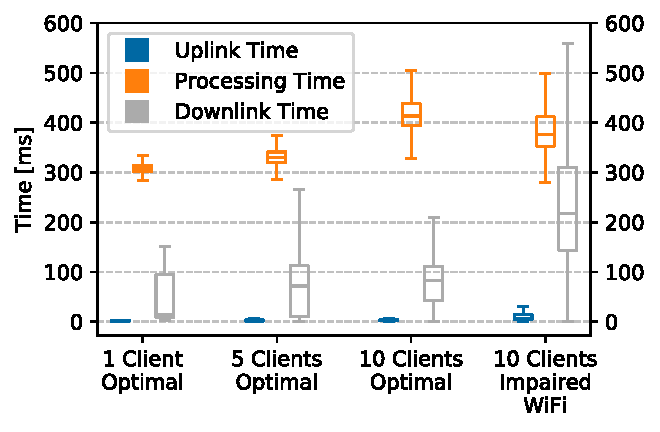
\includegraphics[width=.85\textwidth]{publications/2019EdgeDroid/plots/comparison/nofonts/box_feedback}%
    \caption{Distribution of latency across system components for inputs that triggered a state transition in the task model.}%
    \label{fig:comparison:feedback}%
\end{figure}%
\begin{figure}%
    \centering%
    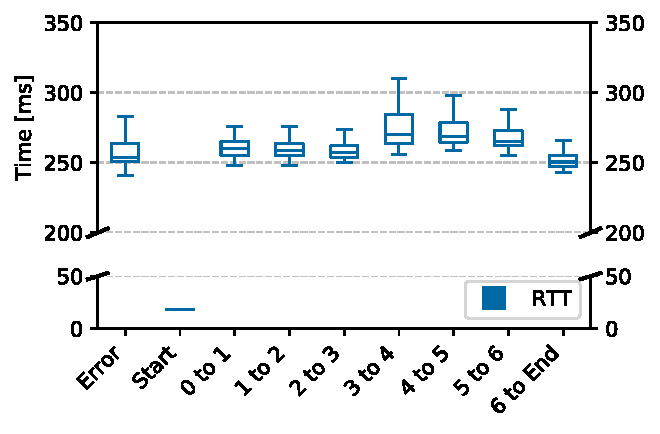
\includegraphics[width=.85\textwidth]{publications/2019EdgeDroid/plots/comparison/nofonts/box_taskstep}%
    \caption{Round-trip-times for input-feedback cycles associated with state transitions in the internal task model for a single client connected over an optimal wireless link.}%
    \label{fig:comparison:tasksteps}
\end{figure}%

The goal of this paper is to provide a methodological approach to studying these latency trade-offs, along with a tool, EdgeDroid 1.0\footnote{We plan to make the EdgeDroid 1.0 benchmarking suite available as Free and Open Source Software and the recorded traces under a Creative Commons License.}, that simplifies the benchmarking of human-in-the-loop applications.
We view EdgeDroid 1.0 to be the very first, and simplest, of a family of tools that will embody increasingly sophisticated and accurate models of user behavior.

Due to the complex nature of the applications and the infrastructure, we opt for experimentally studying the trade-offs in a repeatable and controllable fashion.
This is difficult mainly due to the unpredictable reaction of human users to the feedback from the backend --- a user might very well misinterpret the feedback handed to them.
EdgeDroid 1.0 mimics the operation of human-in-the-loop applications by replaying recorded traces of sensory input.
This sensory information is then processed by the original compute process at the backend, generating feedback.
However, this feedback is not processed by humans, but by a parameterizable model of human reaction.
Through synchronized time tracking at the different processing points of the application, EdgeDroid 1.0 allows for accurate measurements of key performance metrics such as the distribution of delays across the application pipeline.
Analysis of these metrics can be performed down to the individual input sample, allowing us to zoom into the internal model of the application under consideration.
Thus, EdgeDroid 1.0 allows us to illuminate the many latency trade-offs existing at the level of the infrastructure, as well as the level of the application.
It can also be used for debugging and validation, by comparing the expected execution flow of a particular trace with the actual flow during the benchmarking.
To the best of our knowledge, this experimentally-driven benchmarking approach is the first one towards experimental performance characterization and potential optimization of human-in-the-loop applications

\Cref{fig:comparison:rtt} presents a comparison of the total measured round-trip-times (RTTs) both for inputs which caused a state transition and inputs that did not.
Next, \cref{fig:comparison:feedback} shows a comparison of the distribution of latencies across system components for inputs that caused an internal state change in the task model of the application.
We differentiate according to the three main components contributing to latency, namely \emph{uplink} and \emph{downlink transmissions}, and \emph{backend processing}.
Finally, \cref{fig:comparison:tasksteps} depicts the distribution of RTTs for each transition in the internal task model for a single client connected over an optimal wireless link.
These metrics were calculated by recording the measured input-feedback cycle delay corresponding to a change in state within the application.
Thus, for instance, the measurements located at column ``3 to 4'' in the figure correspond to the aggregated round-trip-times for every input-feedback cycle corresponding to a change from state 3 to state 4 within the application task model, for the 100 repetitions of the scenario.

In the following discussion we will refer to inputs which triggered a transition in the task model as \emph{feedback-rich inputs} and those that did not as \emph{feedback-less inputs}.

For the analysis of these results, we will take into consideration the bound of \SI{600}{\milli\second} response time for step-by-step task-guidance derived by the authors of~\cite{Chen:AnEmpiricalStudyOfLatency}.
This bound marks the point after which further delays in the delivery of feedback to the user start to negatively affect user experience, and allows for a straightforward evaluation of the responsiveness of the system.

We will begin our analysis of the experiment results with \Cref{fig:comparison:rtt}.
These results present a stark contrast in the round-trip-times for inputs which cause a state transition versus inputs that do not, with RTTs for the former being up to an order of magnitude greater.
It's worth mentioning though that responses to feedback-less inputs are invisible to the user, and are just included here as a sort of baseline to compare feedback-rich round-trip times with.

We can identify a pair of interesting effects in the scaling of the task-guidance WCA application.
One, scaling behavior for the application seems to be linear with respect to the number of clients.
Two, in the case of the impaired WiFi, the effect on the feedback-rich inputs is very pronounced, with the average of the RTTs for these inputs being over the previously discussed bound of \SI{600}{\milli\second}.

It is worth noting that already at just 10 clients the response times for feedback-rich inputs are very close to the bound.
Looking at this through the lens of a an application developer, it could hint at a need for optimization of the later parts of the application pipeline, since RTTs for inputs which are discarded in the detection stage of the pipeline (i.e.\ feedback-less inputs) are still well below \SI{200}{\milli\second}.

EdgeDroid 1.0 allows researchers to zoom into specific components of the application feedback loop, as exemplified by \cref{fig:comparison:feedback}.
From this figure it is clear that the main component which contributes to latency in the optimal case is the backend processing, further lending credibility to our previous comment on the need for optimization.
Nevertheless, when the link quality decreases, the delays on the downlink start to overshadow the delays on the processing.
Here, the downlink time sometimes almost reaches the ideal bound by itself.
A system designer might then conclude from this that in order to be able to scale the application, their focus needs to be on improving the quality of the wireless link before increasing the processing power on the backend.

Finally, EdgeDroid 1.0 allows even more insights to be gained by homing in to individual steps in a task-guidance WCA. Consider \cref{fig:comparison:tasksteps}.
The figure shows clears spikes in latencies at the transitions from task state 3 to 4 and from task state 4 to 5, which could indicate to the application developer that these specific transitions are ripe for optimization.


\todo[inline]{\cref{paper:olguinmunoz2019edgedroid}}\label{summary:2019edgedroid}

\subsection{Applying the methodology to \acsp{NCS}}\label{ssec:methodology:ncs}

\todo[inline]{\Cref{paper:olguinmunoz2022cleave} implements both the methodology and the tool.}

\begin{figure*}
    \centering
    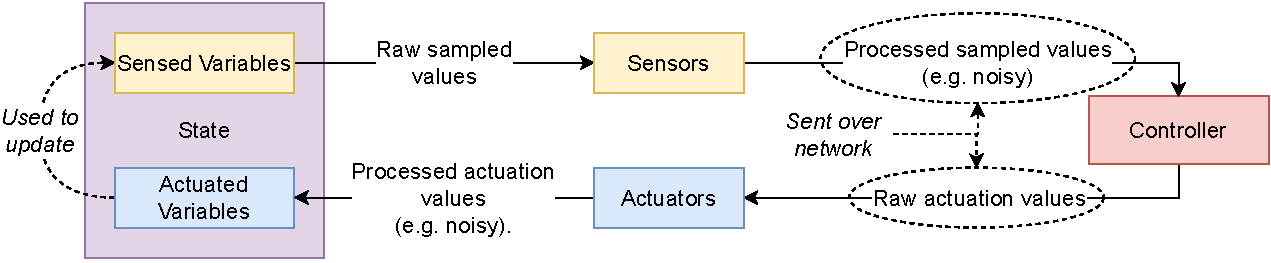
\includegraphics[width=.8\textwidth]{publications/2022CLEAVE/images/CLEAVE_NCS_structure}
    \caption{
        Structure of an emulated \acl*{NCS} in \acs*{CLEAVE}.
    }\label{fig:cleave:ncs:struct}
\end{figure*}

We overcome this issue by proposing a completely virtual plant allowing for unparalleled flexibility in changing the plant model and characteristic features of the experiments.
In this paper, we present the first fully-software-based framework for scalable and repeatable benchmarking of edge-native \ac{NCS}.
As edge computing begins being adopted by industry, more and more variations have begun to appear in literature.
``Near'', ``far'', ``core'', and ``telco'' edge describe variations of the original concept and are becoming ubiquitous in new research.
While the core idea of edge computing is widely accepted as fundamental for pervasive \acp{NCS} in general, understanding the strengths and weaknesses of such different edge concepts is of paramount importance.

Our framework, \ac{CLEAVE}, aims to simplify the repeatable and scalable benchmarking of such systems.
It is fully virtualized, inspired by our previous work on benchmarking human-in-the-loop applications on the edge~\cite{Olguin2019EdgeDroid}.
The tool consists of a benchmarking framework and software development kit for the development of emulated physical systems and softwarized controllers.
These virtual \acp{NCS} can then be deployed on real networks for reparametrizable, repeatable, and reproducible benchmarking of the complete system.

\ac{CLEAVE} is built using \emph{Python 3.8}, making it highly extensible and able to harness the multitude of already existing user libraries.
It is furthermore compatible with container technologies such as \emph{Docker}\footnote{Docker Engine: \url{https://www.docker.com/}}, making it suitable for automated deployment, scaling, and benchmarking on industry-standard edge setups using container orchestration solutions.

In this work, we aimed to tackle this issue through a fully software-based framework for repeatable, reproducible, and easily scalable \ac{NCS} benchmarking with a particular focus on edge deployment.
We argue our approach, \ac{CLEAVE}, embodies a better solution than previous work for a number of reasons:
\begin{enumerate}
    \item Compared to fully physical approaches, such as those used in\ \cite{Baumann2018LowPower} and\ \cite{Cuenca2019UAV}, our approach allows for greater flexibility and scalability.
          The aforementioned approaches rely on specialized and sometimes entirely custom-built physical platforms, and although flexible and cheap approaches such as Zoppi \emph{et al.'s} --- which uses a LEGO-based physical plant --- exist, these still do not reach the level of flexibility afforded by a fully software-based framework.
          Experimenters still need copies of the hardware, making anything other than small-scale setups unfeasible.
          In contrast, our approach requires only general-purpose computing platforms, and can be employed by basically anyone with access to a computer.
          Scalable deployments can in turn easily and cheaply be set up using single-board computers and/or virtual cloud instances.
    \item When compared to simulated approaches such as\ \cite{Ma2019DynamicSched}, \ac{CLEAVE} provides a higher level of realism, in particular with regards to the network segment of the system.
    \item Finally, although it shares much in common with previous emulated approaches such as the one employed in\ \cite{Wang2020VoltageControl}, \ac{CLEAVE} has an advantage by specifically targeting a general-purpose approach using industry-standard, cloud- and edge-native tools and software.
          The tool can easily be deployed and scaled using widely-used frameworks such as Docker Swarm and Kubernetes.
\end{enumerate}

We validate the utility of this tool through an example use case approximating a proposed edge deployment of inverted pendula control loops co-located with video analytics services.
We argue such a use case represents a realistic scenario and appropriate benchmark for the tool, since
\begin{enumerate*}[itemjoin={{; }}, itemjoin*={{; and }}]
    \item the inverted pendulum plant is ubiquitous in \ac{NCS} research
    \item similar setups exist in real-world industrial use
    \item video analytics has long been proposed as a ``killer app'' for edge computing.
\end{enumerate*}
Our results showcase the ability of the framework to extract relevant metrics relating to the stability of the control system, as well as on the performance of the underlying network link.
We believe \ac{CLEAVE} represents an important step towards enabling inexpensive and low-complexity scalable research for real-world deployment of edge-bound \acp{NCS}.

\todo[inline]{Some plots and results}

\begin{figure}
    \centering
    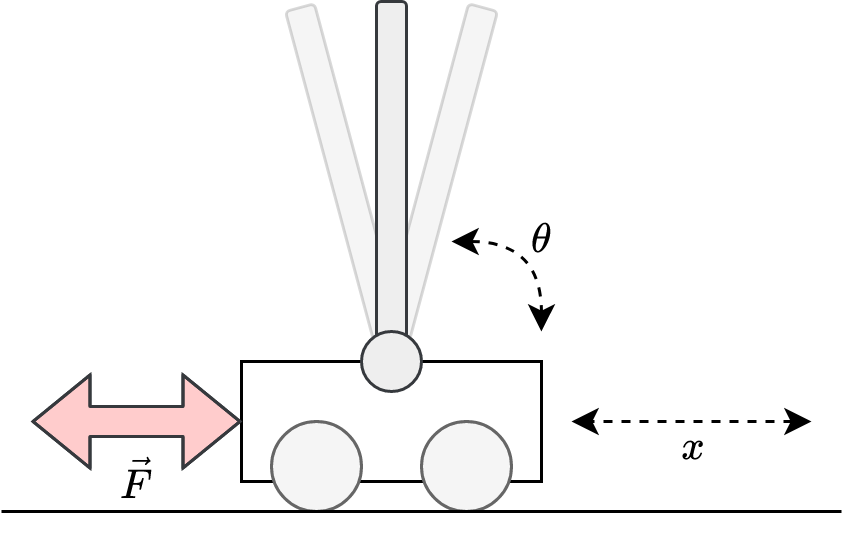
\includegraphics[width=.6\textwidth]{publications/2022CLEAVE/images/inverted_pendulum.png}
    \caption{
        The 2D inverted pendulum system.
    }\label{fig:invpend}
\end{figure}

\begin{figure}[t]
    \centering
    \begin{subfigure}[h]{.22\textwidth}
        \centering
        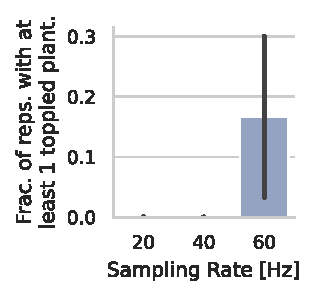
\includegraphics[width=\textwidth]{publications/2022CLEAVE/plots/fixed_video_topple_frac}
        \caption{Toppled plants.}\label{fig:video:toppled}
    \end{subfigure}%
    \hfill%
    \begin{subfigure}[h]{.22\textwidth}
        \centering
        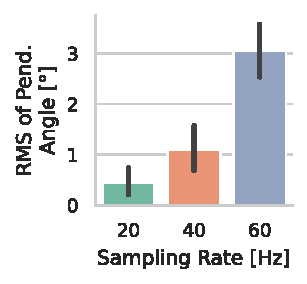
\includegraphics[width=\textwidth]{publications/2022CLEAVE/plots/fixed_video_angle_rms}
        \caption{Angle \ac{RMS}.}\label{fig:video:rms}
    \end{subfigure}\\
    \begin{subfigure}[h]{.22\textwidth}
        \centering
        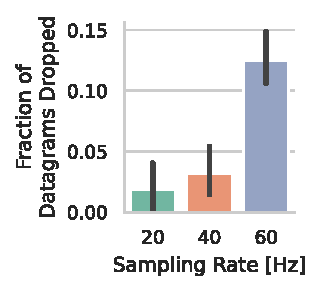
\includegraphics[width=\textwidth]{publications/2022CLEAVE/plots/fixed_video_drop_frac}
        \caption{Packet losses.}\label{fig:video:drop}
    \end{subfigure}%
    \hfill%
    \begin{subfigure}[h]{.22\textwidth}
        \centering
        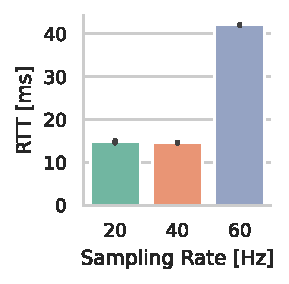
\includegraphics[width=\textwidth]{publications/2022CLEAVE/plots/fixed_video_rtt}
        \caption{\acsp{RTT}.}\label{fig:video:rtt}
    \end{subfigure}%
    \caption{
        Multi-loop, resource-constrained setup results.
        Error bars indicate \SI{95}{\percent} \acp{CI} in all plots.
    }\label{fig:video:results}
\end{figure}

\FloatBarrier%

\subsection{Orchestrating experimentation in edge computing testbeds}

\todo[inline]{\cref{paper:olguinmunoz2022ainur} describes a software framework for testbeds used for the methodology described in this thesis}

In this work, we present our solution to the challenge of testbed automation: Ainur, a framework for wireless testbed automation with a specific focus on end-to-end experimental research in the context of edge-computing using cloud- and edge-native technologies.
Ainur is designed to deploy experimental runs from a workload perspective by configuring the physical testbed, initializing all involved software components, deploying and executing the experimental workload, collecting logs and data, and finally gracefully degrading the system.
The framework allows for dynamic, software-definition of physical and logical links, network topology, cloud and edge computing resources, as well as experimental workload deployment and orchestration.
It heavily leverages cloud-native technologies, such as Docker containers, in order to support a wide variety of different testbed hardware setups and experimental configurations and workloads, as well as to be as easily extendable as possible.
Furthermore, we make Ainur available to the community as \ac{FOSS}.
It can be obtained from the {KTH-EXPECA/Ainur} repository on GitHub~\cite{ainur:github}, released under an Apache version \num{2.0} license.

In this paper, we have introduced a framework for repeatable end-to-end testbed automation in the context of wireless networking and edge computing research.
Named Ainur, it simplifies the execution and verification of end-to-end experimentation by automating the
\begin{enumerate*}[itemjoin={{; }}, itemjoin*={{; and }}]
    \item establishment of physical links between hosts, including the configuration of complex wireless systems such as 4G \ac{LTE} and 5G
    \item provisioning of and connection to remote cloud instances
    \item initialization of \ac{IP} layer connectivity between hosts
    \item collection of logs and data
    \item deployment, scaling, and lifecycle management of containerized processes
\end{enumerate*}.
We have described its general architecture, which follows a layered design mimicking the network stack layers the framework directly interacts with, as well as the underlying assumptions about its deployment environment and specific requirements for its deployment.
We have also outlined a demonstration which showcases the flexibility and power of the framework by deploying two different workloads to our testbed.
We believe our framework represents an important step towards repeatable, replicable, yet low-access barrier end-to-end wireless testbed experimentation.
It has been released as \ac{FOSS} and can be found on GitHub~\cite{ainur:github}.\\

\todo[inline]{Some plots}

\begin{figure}[t]
    \centering
    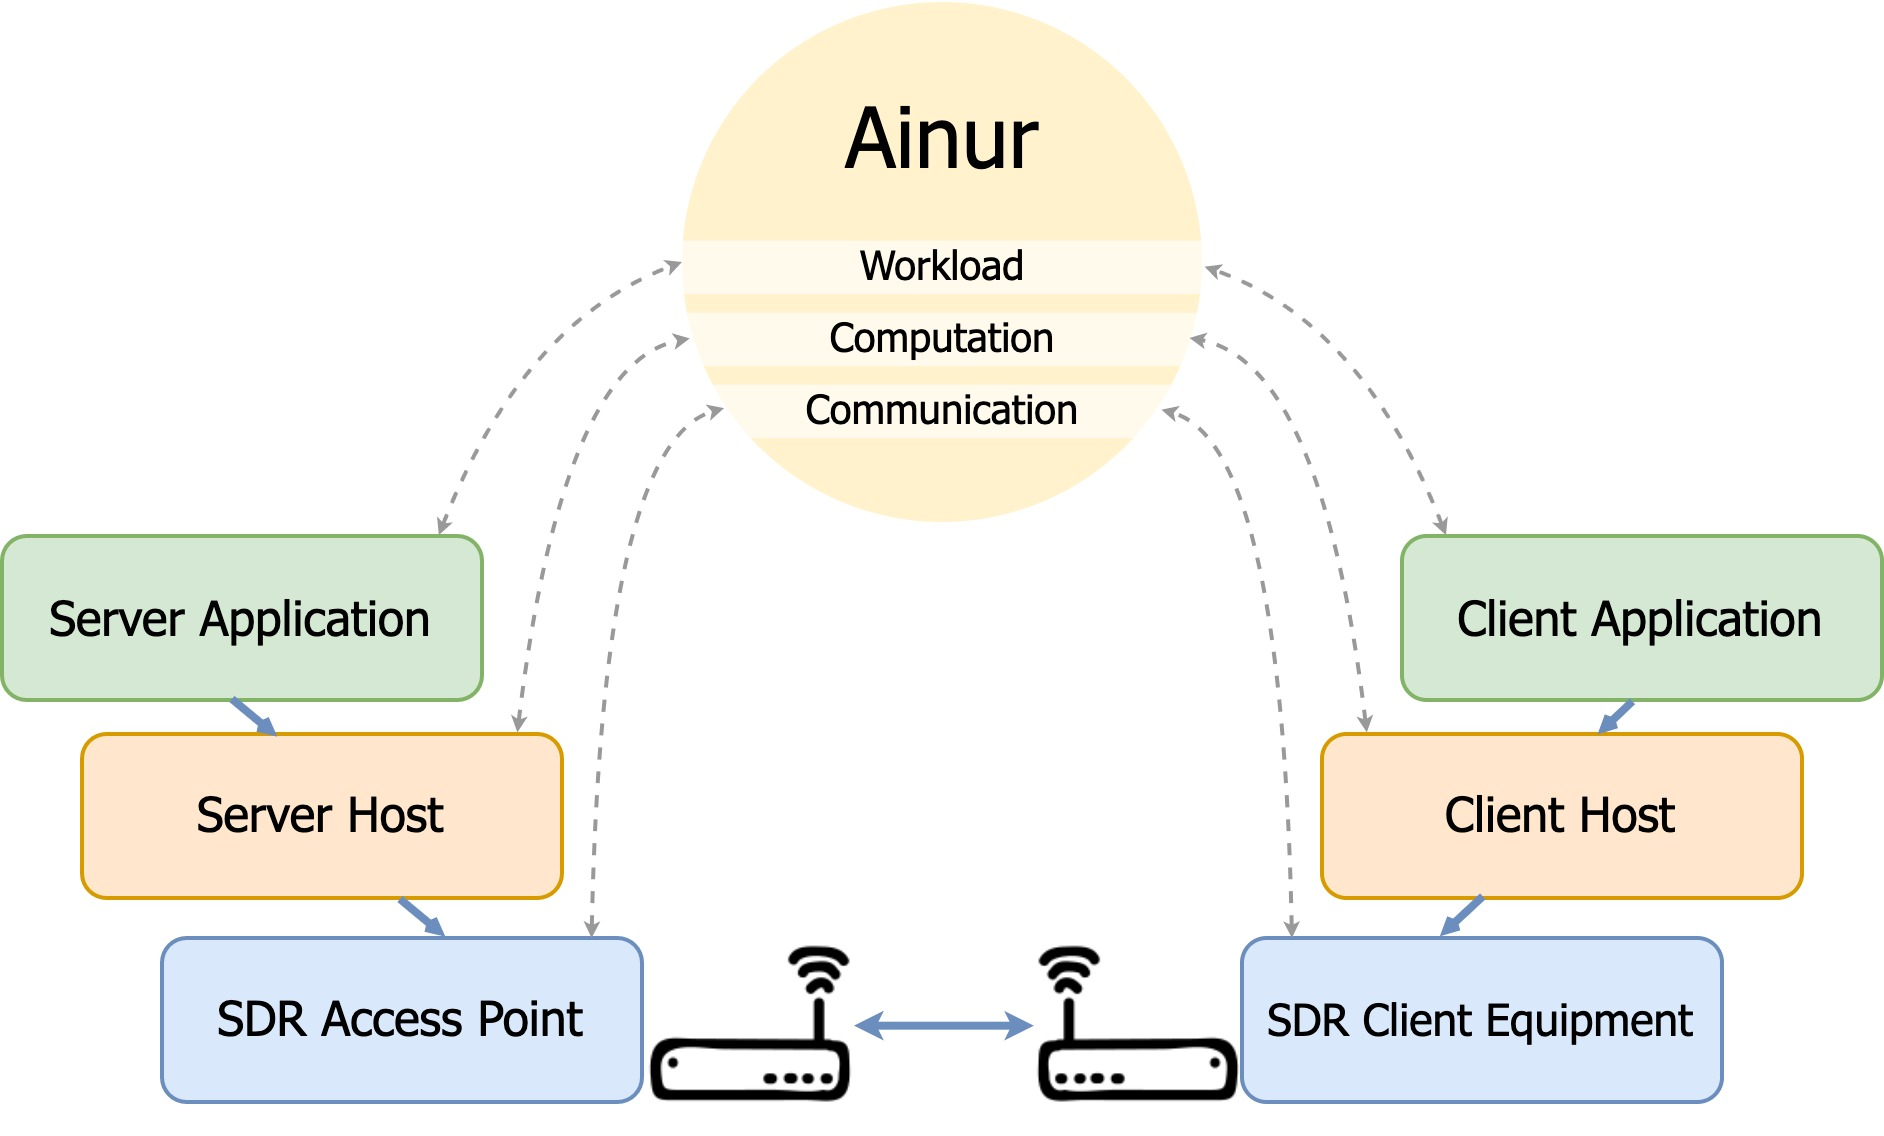
\includegraphics[width=0.9\linewidth]{publications/2022Ainur/figures/overview.jpg}
    \caption{Layered structure of an Ainur experiment}\label{fig:overview}
\end{figure}

\begin{figure*}
    \centering
    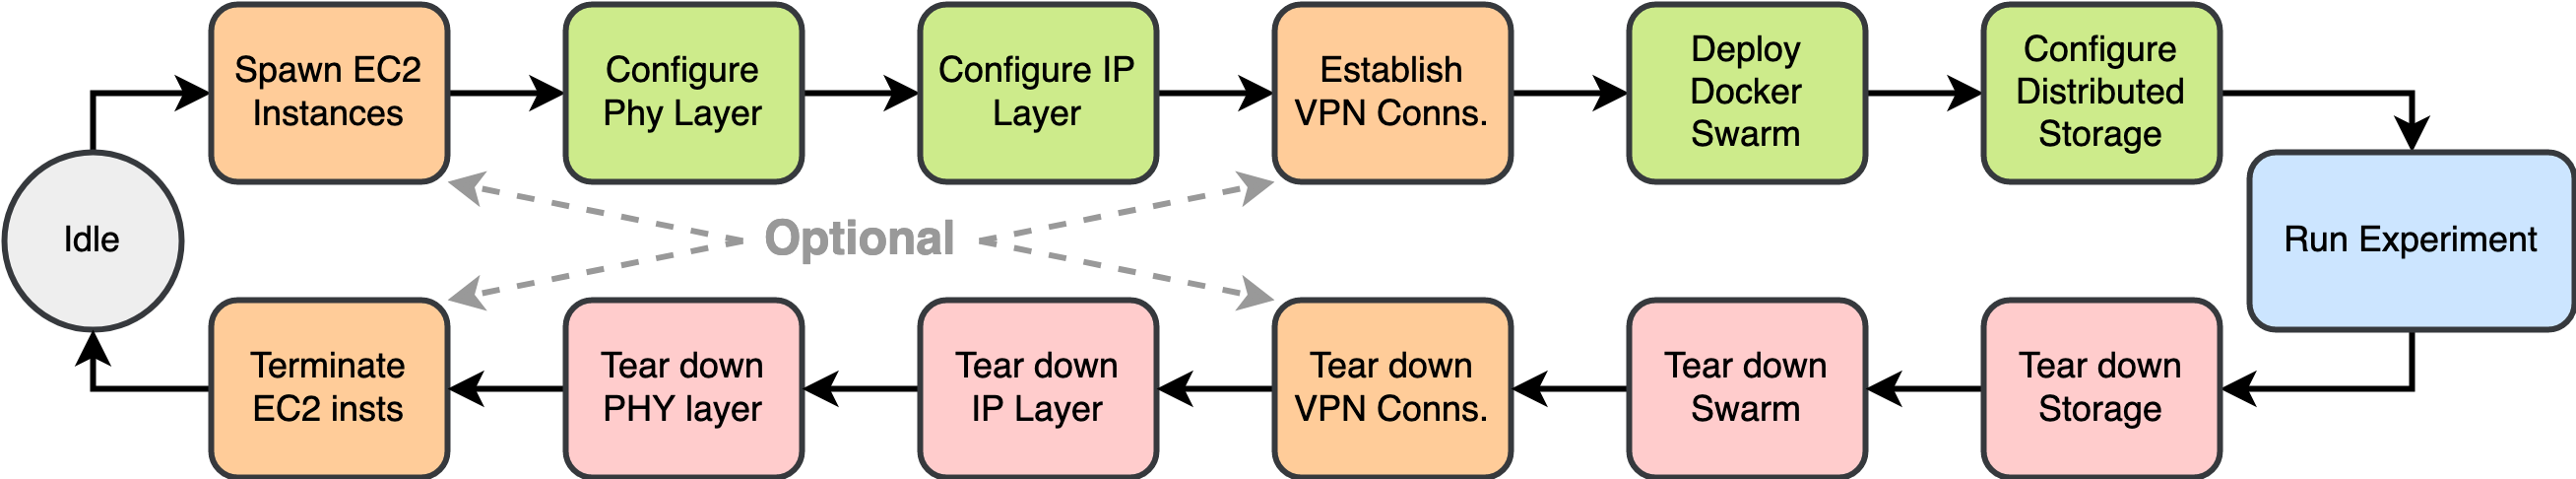
\includegraphics[width=0.8\textwidth]{publications/2022Ainur/figures/flow2.png}
    \caption{Lifecycle of an experimental run in Ainur. Blocks in orange are optional.}\label{fig:flow}
\end{figure*}

\begin{figure*}
    \centering
    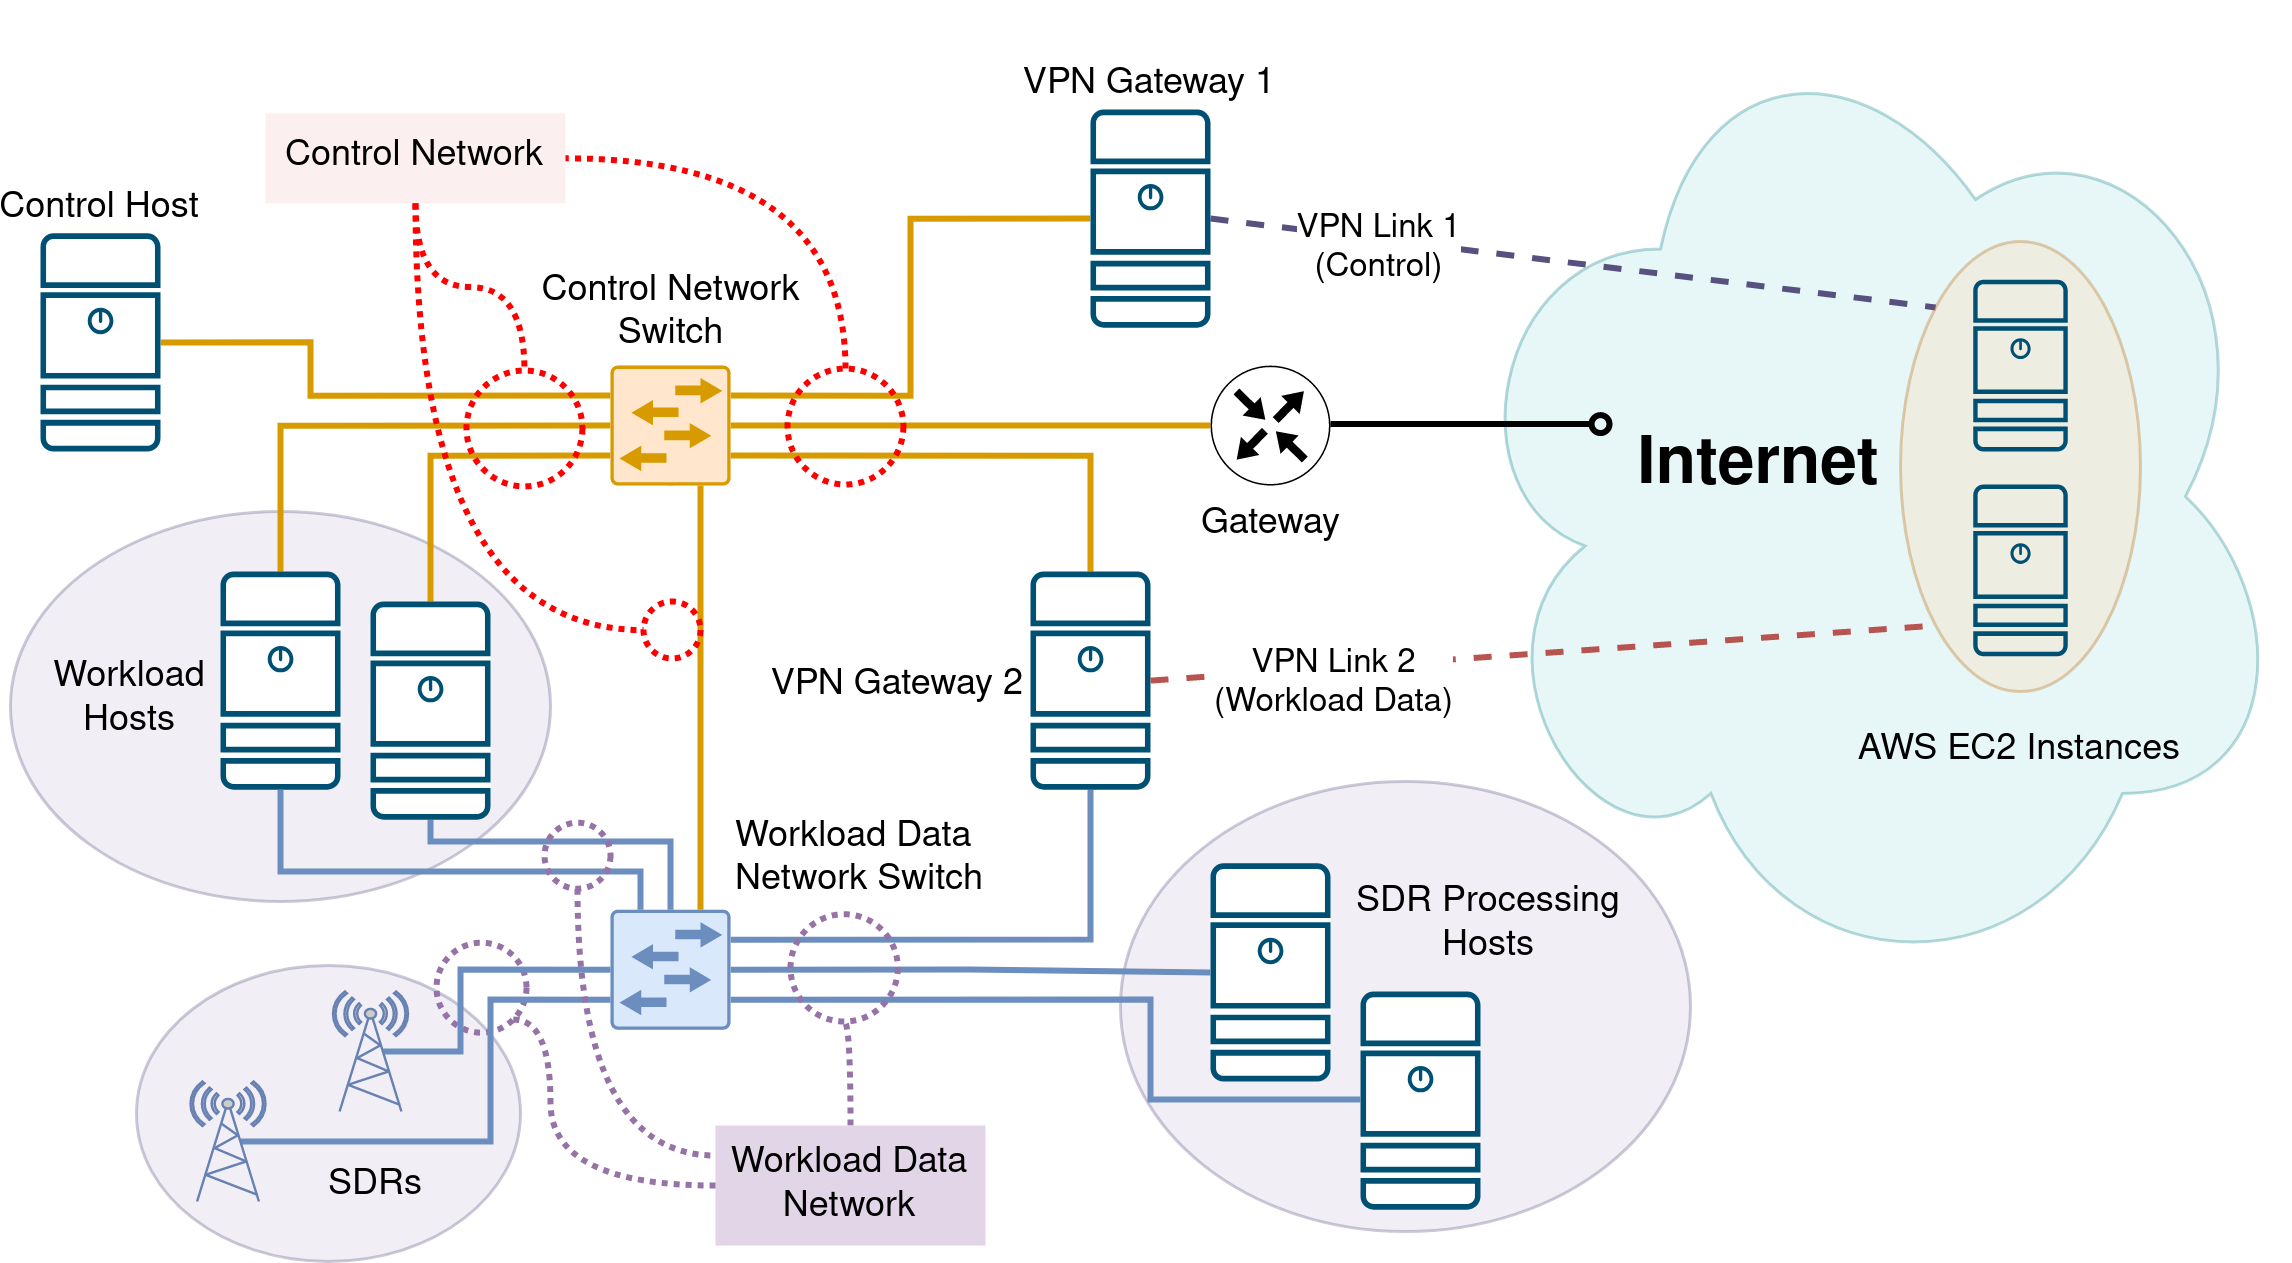
\includegraphics[width=.8\textwidth]{publications/2022Ainur/figures/network.png}
    \caption{Network structure assumed by Ainur.}\label{fig:network}
\end{figure*}

\section{Extending the methodology in the context of \acs{WCA}}

\subsection{Characterizing human behavior}

\todo[inline]{\cref{paper:olguinmunoz2021impact} describes the acquisition of the necessary data and insights for the models.}

\todo[inline]{From introduction}

We intended to answer four core research questions relating to human responses to decreased application responsiveness.

\begin{itemize}
    \item \emph{Do subjects change the temporal profile of their actions in relation to system latency?}

          In line with previous research in this area, we expected subjects to change their temporal profiles as system responsiveness decreased.
          The extent or form of these changes were however unknown.
          We also hypothesized that large enough drops in responsiveness could lead to complete abandonment of the task by subjects.

          Our results show an emergent pacing effect on user actions as system responsiveness is reduced.
          While it would seem self-evident that users take longer to complete a task while using a system with low responsiveness --- as they have to wait longer for new instructions --- our study found that user slow-down represents a source of substantial additional delay.
          To be more precise, the data indicate that users slow down not only because they have to wait for the system to catch up, but that their reactions to new instructions is also delayed.
          Moreover, this effect scales with the decrease in responsiveness and remains for a while, even after system responsiveness improves.

    \item \emph{Do subjects show signals of arousal in physiological responses to changes in system latency?}

          We hypothesized subjects would show signs of stress and frustration as system latency increased, due to the added annoyance of dealing with an unresponsive system.

          The results we present, however, seem to refute this hypothesis.
          We were not able to detect any significant effects on the physiological signals obtained from the biometric sensors as system responsiveness was altered.

    \item \emph{Are responses to delay effects in subjects mediated by cognition and/or emotion?}

          In line with previous items, we expected delay effects in subjects to be mediated primarily by emotion.
          In particular, we expected emotional effects to be correlated with the strength of the added delay.

          The results point in a different direction though, indicating that reduced responsiveness in WCA systems leads to a disruption of participants' cognitive plan for the task and not to an emotional response.
          This is evidenced by the previously discussed pacing effect and the lack of significant physiological responses.

    \item \emph{Are these effects mediated by personality indicators in any way?}

          Finally, we hypothesized that the individual trait of \emph{neuroticism}~\cite{john1999:bfi} would play a role in mediating these effects, as it has previously been connected to intolerance for time delay~\cite{hirsh2008delay}.
          We also expected \emph{focus} and \emph{involvement}~\cite{witmer1998:itq} to play roles in this.

          The results obtained agree with our hypothesis.
          We found significant effects of neuroticism on the responses exhibited by subjects, and all three traits were found to play a role through factor analysis.

\end{itemize}

% Our results indicate that reduced responsiveness in WCA systems leads to a disruption of participants' cognitive plan for the task.
% This is evidenced by an emergent pacing effect on user actions as system responsiveness is reduced.
% While it would seem self-evident that users take longer to complete a task while using a system with low responsiveness --- as they have to wait longer for new instructions --- our study found that user slow-down represents a source of substantial additional delay.
% To be more precise, the data indicate that users slow down not only because they have to wait for the system to catch up, but that their reactions to new instructions is also delayed.
% Furthermore, this effect persists for a while after system response improves and is modulated by intrinsic personality traits, in particular, \emph{neuroticism}~\cite{john1999:bfi}. 

We believe that these results provide concrete and relevant implications for WCA design, deployment, and optimization.
One example is the behavioral slow-down, as it extends application runtime significantly, and thus has clear and direct implications for resource and power consumption.
Another is the fact that the adverse effects of delay on users do not immediately subside as delay is diminished --- this has potential consequences for resource allocation strategies.
Moreover, in multi-user scenarios, the dependency of user slow-down effects on delay mean efficient resource allocation across applications potentially looks different from what could be considered ``fair''.

Our hope is that the results we provide might prove useful for the understanding and optimization of deployments of WCA.\@
These results represent unexpected, valuable findings, which can be employed to model and understand how users interact with latency in applications and systems, and develop resource allocation and power optimization strategies.
Additionally, we hope that the results we provide might pave the way for the improvement of performance evaluation tools such as our previous work in \cite{olguin:2018, olguin:2019}.
Such systems would greatly benefit from this knowledge, as it would allow for the design and implementation of realistic models of human behavior, making highly accurate benchmarks a reality in the domain of WCA.\@

\todo[inline]{From discussion}

We start our discussion with the main results of our experimentation presented in the previous section:

\begin{itemize}
    \item Firstly, and perhaps most importantly, we find that a system slow-down induces an \textit{additional} behavioral slow-down.
          That is, as system responsiveness decreases, our data indicates that users significantly slow-down in their execution of the task.
          This slow-down scales with the decrease in responsiveness; compared to the no-delay case, participants were on average \SI{12}{\percent} slower at \SI{1.65}{\second} delay and \SI{26}{\percent} at \SI{3.0}{\second} delay.
          Moreover, there is a temporal component to this effect; users become progressively slower the more time passes with reduced system responsiveness.

    \item Secondly, we find that the effects of behavioral slow-down due to impaired system responsiveness \emph{remain} for at least a few steps after system responsiveness improves.
          This is evidenced by the longer per-step-execution times of the first four steps of blocks immediately following a high-delay block, as pictured in \cref{fig:exectime:transition}.
          The question of whether any lingering effect can be measured after these four steps remains open.

    \item Thirdly, we evidence a speed-up in execution time over a series of steps; that is, subjects get faster at performing steps as the task progresses.
          However, the strength of this effect decreases as delay increases.
          Whereas for blocks without delay users performed the last four steps of a 12-step block on average \SI{36}{\percent} faster than the first four, at the maximum delay this effect practically disappears.

    \item Fourthly, in terms of inter-subject differences, PCA revealed three main factors governing users' response to delay.
          The first factor represents sensitivity to delay as moderated by the ``Big Five'' personality trait of neuroticism and both measures of immersion: focus and involvement.
          Factor two and three represent dedication to the task as opposed to delay intolerance and reflect variables related to attentiveness, respectively.
          In simple terms, these results suggest that the effects of delay are most potent in individuals who are sensitive and involved in the task.
          The findings appear selective to cognitive assistance tasks like the present ones, inasmuch as the same measures did not correlate with outcomes in other computer-intensive environments such as immersive VR~\cite{quesnel2018you}.
          These correlations are also consistent with previous findings indicating that individuals scoring high in neuroticism tend to be intolerant to delayed reward~\cite{hirsh2008delay}.
\end{itemize}

A central question therefore arises: to which physio- and psychological mechanisms can these findings, most importantly the substantial slow-down in task execution, be attributed?

In \cref{sec:background}, we initially considered the possibility that delays might produce negative emotional reactions.
These could in turn elicit generalized arousal.
We also postulated that adapting to delay might progressively deplete cognitive resources in users.
However, the present data provide relatively little support for these alternatives, in that the predicted measures did not produce the expected statistical trends.
Specifically, physiological measures of GSR and HR failed to show evidence of differential arousal under long vs.\ short delays, and speed-induced errors and non-completions predicted by resource depletion were not observed.
The acceleration data further did not indicate that extended delay significantly increases erratic movement.
% physiological measures of GSR and HR failed to show evidence of differential arousal under long vs.\ short delays, and speed-induced errors and non-completions predicted by resource depletion were not observed.
% The acceleration data further do not indicate that extended delay increases erratic movement.
To the contrary, the data suggest this effect results from a delay in movement after an instruction is introduced.
That is, users fail to capitalize on the new information as quickly as they could.
Thus, contrary to our preliminary postulations, behavioral effects seem to arise from impaired cognitive control mechanisms, and not from emotion or resource depletion.
We hypothesize that the effects of feedback latency can best be understood as changes in the use of a cognitive plan.
As was described in \cref{sec:experimentaldesign,fig:lego:hierarchical}, complex cognitive and motor tasks have been modeled as the unfolding of a hierarchy of command, from high-level plans to physical output.
Long system latencies, we propose, disrupt the automating of such a plan, instead relegating it to attention-based control at the step-by-step level that is easily diverted.
This also provides a possible explanation for the lingering effects of delay after an acceptable system responsiveness is restored, as users needs time re-adjust and re-automate their cognitive plans.

As to the applicability of our findings to other applications, it must be noted that these results pertain to a specific class of applications, namely step-based task-guidance WCA.\@
However, we would expect our findings to extend to similar applications, as long as they follow the same pattern of seamless interaction --- i.e.\ such that the user does not need explicitly interact with the application to advance the state.

The results here presented provide a number of possible implications for WCA system design and optimization, both for single and multi-application flows.

\begin{itemize}

    \item Due to the behavioral slow-down in users, even short-term reductions in responsiveness will lead to significantly extended application lifetimes.
          This has direct implications for resource and power consumption.

    \item The fact that the adverse effects of delay on users do not immediately disappear as the system returns to a high-responsive state could have unconventional consequences for resource allocation.
          This is of particular importance, for instance, for cases where the user may be able to finish the task before these effects subside.
          In such cases, the limited potential gains might not justify diverting valuable system resources to the impaired application.

    \item In multi-user environments, the time dependency of user slow-down effects mean that fair degradation of system responsiveness across applications may not ultimately be beneficial to the system as a whole.
          Take for instance two applications on the same system which negatively interfere with each other.
          The longer they interfere with each other, the longer their respective lifetimes are going to be, which in turn causes them to interfere even longer, potentially entering a positive feedback loop.
          In such a case, prioritizing one over the other rather than trying to improve responsiveness for both might lead to resources being freed up faster system-wide.

    \item Based on our findings relating individual differences between users and their sensitivity to delays, it might also be possible to extrapolate user characteristics from measured execution times.
          This could prove a valuable tool for load balancing, for instance by prioritizing resource allocation to users with a higher sensitivity to system-state degradation.
          However, this remains an open challenge.

\end{itemize}

To wrap up, we believe the present data provide novel and unexpected insights for the understanding and optimizing of WCA deployments.
Although more subtle than expected, and in some cases somewhat counterintuitive, these insights represent a valuable tool to tackle inefficiencies in these systems.
Moreover, we also argue these findings represent a first step towards a full-fledged understanding of the relationship between application responsiveness and human behavior.
More research in this area will surely uncover more complex and interesting behaviors.
Finally, we believe the data provide parameters that can usefully be integrated into cognitive models of WCA that might be constructed under existing architectures like ACT-R.
These same parameters could be used to modulate the timing and generation of inputs in trace-based workload generation tools such as the EdgeDroid platform~\cite{olguin:2018,olguin:2019}, allowing the tool to use the same trace to generate workloads for a multitude of different user profiles.

\todo[inline]{Some diagrams, plots, and results}

\begin{figure}[h]
    \centering
    \begin{subfigure}[t]{.49\textwidth}
        \centering
        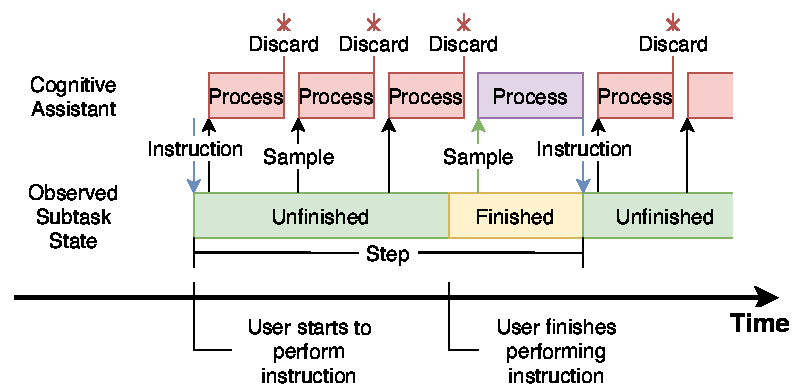
\includegraphics[width=\textwidth]{publications/2021ImpactDelayedResponse/Fig4a.eps}
        \caption{Structure of a step in a generic cognitive assistance application.
            The assistant provides an instruction to the user and continuously samples the step state; inputs captured while the step is unfinished are silently ``discarded'' (i.e.\ they do not cause the generation of a new instruction).
            % by the assistant, as they do not contain relevant information.
            Once the user finishes performing the step, the next sample \emph{will} cause the generation of a new instruction.
            % which will subsequently be provided to the user.}%
        }
        \label{fig:cogassist:step}
    \end{subfigure}%
    % \medskip%
    \hfill%
    \begin{subfigure}[t]{.49\textwidth}
        \centering
        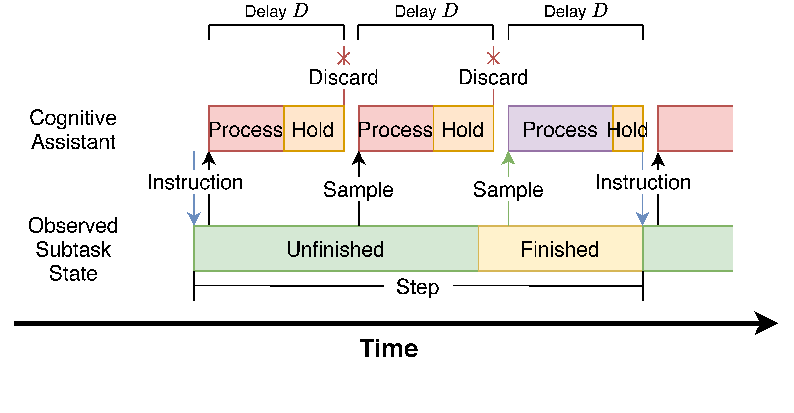
\includegraphics[width=\textwidth]{publications/2021ImpactDelayedResponse/Fig4b.eps}
        \caption{In the experimental task, an additional variable segment of time is introduced immediately following the processing of the input frame in order to extend the perceived processing time of the input to a specific target delay.}%
        \label{fig:cogassist:step:delay}
    \end{subfigure}
    \medskip%
    \begin{subfigure}[t]{.49\textwidth}
        \centering
        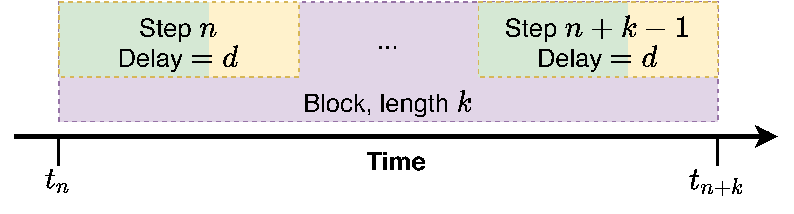
\includegraphics[width=\textwidth]{publications/2021ImpactDelayedResponse/Fig4c.eps}
        \caption{Structure of a block in the experimental task.}%
        \label{fig:cogassist:block}
    \end{subfigure}%
    % \medskip%
    \hfill%
    \begin{subfigure}[t]{.49\textwidth}
        \centering
        \includegraphics[width=\textwidth]{publications/2021ImpactDelayedResponse/Fig4d.eps}
        \caption{Visualization of the execution time of a step.}%
        \label{fig:exectime:diagram}
    \end{subfigure}%
    % \medskip%
    \caption{Components of the cognitive assistance task.}
\end{figure}

\begin{figure}[h]
    \centering
    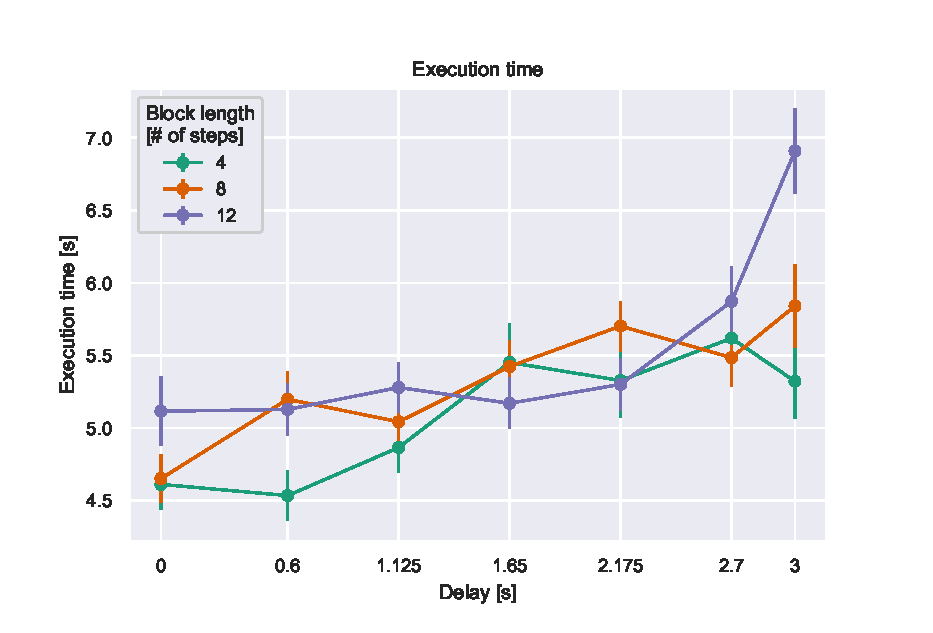
\includegraphics[width=.8\textwidth]{publications/2021ImpactDelayedResponse/Fig6.eps}
    \caption{Per-step execution time by block length vs.\ delay. Error bars indicate the Standard Error of the Mean (S.E.M.)}\label{fig:exectime}%    
\end{figure}

\begin{figure}[h]
    \centering
    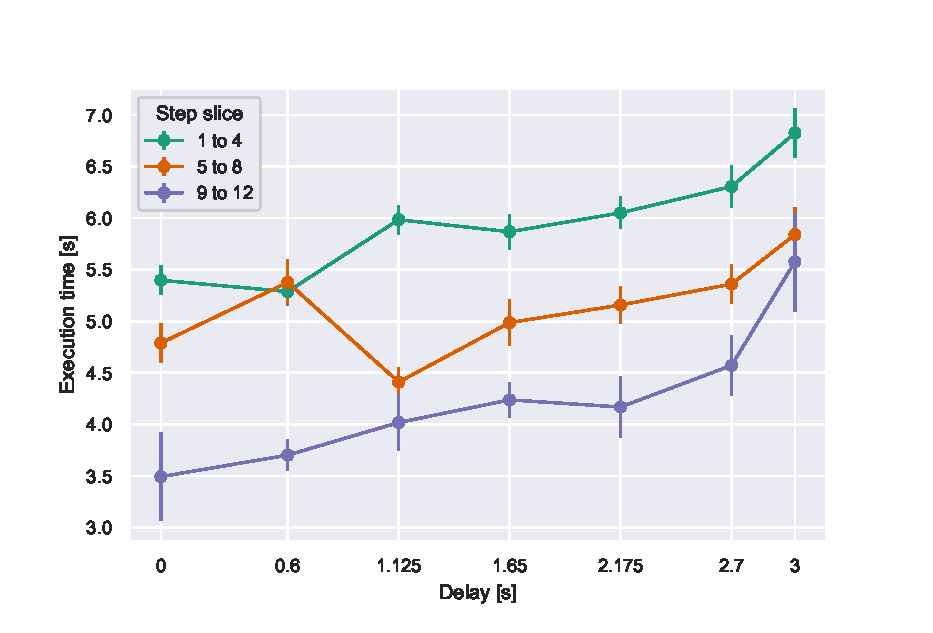
\includegraphics[width=.8\textwidth]{publications/2021ImpactDelayedResponse/Fig7.eps}
    \caption{Mean per-step execution time vs.\ delay, by step slice.
        Error bars indicate S.E.M.}
    \label{fig:exectime:delay:slice}
\end{figure}

\begin{figure}[h]
    \centering
    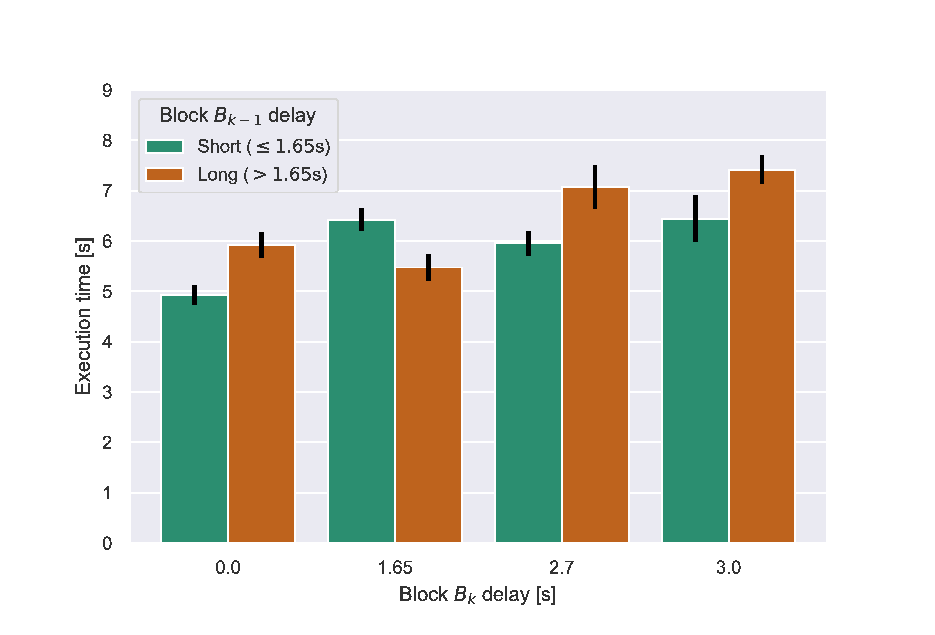
\includegraphics[width=.8\textwidth]{publications/2021ImpactDelayedResponse/Fig8.eps}
    \caption{Per-step execution time across the first four steps after a block transition from block \( B_{k-1} \) to \( B_k \). Error bars indicate S.E.M.}\label{fig:exectime:transition}%
\end{figure}

\begin{table}[h]
    \centering
    \caption{Principal Component Analysis}\label{tab:pca}
    \begin{subtable}[h]{\textwidth}
        \centering
        \caption{Main components identified.}
        \setlength{\tabcolsep}{0pt} % let TeX compute the intercolumn space
        \begin{tabular*}{\textwidth}{@{\extracolsep{\fill}\quad}lrrr@{}}
            \toprule
            \textbf{Factor} & \textbf{Comp. 1} & \textbf{Comp. 2} & \textbf{Comp. 3} \\
            \midrule
            BFI Conscientiousness                  & \textcolor{lightgray}{\( -0.022 \)} &                         \( 0.668 \) & \textcolor{lightgray}{\( -0.481 \)} \\
            BFI Neuroticism                        &                         \( 0.600 \) &                        \( -0.678 \) & \textcolor{lightgray}{\( -0.118 \)} \\
            ITQ Focus                              &                         \( 0.678 \) &  \textcolor{lightgray}{\( 0.203 \)} &                         \( 0.504 \) \\
            ITQ Involvement                        &                         \( 0.573 \) &                         \( 0.540 \) &  \textcolor{lightgray}{\( 0.417 \)} \\
            Exec. Time (delay 3.0 s, length 12)    &                         \( 0.758 \) & \textcolor{lightgray}{\( -0.178 \)} & \textcolor{lightgray}{\( -0.348 \)} \\
            Log EEG power \( \alpha + \beta \) Slice 1 & \textcolor{lightgray}{\( -0.436 \)} & \textcolor{lightgray}{\( -0.251 \)} &                         \( 0.589 \) \\
            \bottomrule
        \end{tabular*}
    \end{subtable}
    \newline
    \medskip
    \newline
    \begin{subtable}[h]{\textwidth}
        \centering
        \caption{Percentages of variance explained by the components.}
        \begin{tabular*}{\textwidth}{@{\extracolsep{\fill}\quad}lrrrr@{}}
            \toprule
            {} & \textbf{Comp. 1} & \textbf{Comp. 2} & \textbf{Comp. 3} & \textbf{Total} \\
            \midrule
            Explained Variance & \SI{31.88}{\percent} & \SI{22.22}{\percent} & \SI{19.03}{\percent} & \SI{73.13}{\percent} \\
            \bottomrule
        \end{tabular*}
    \end{subtable}
\end{table}

\subsection{Emulating human behavior}

We introduce the first, to our knowledge, data-driven model for human timings in \ac{WCA} applications.
Using the data collected for \textcite{olguinmunoz:impact2021} as a base, we build a stochastic model which takes as input past measurements of system responsiveness and produces realistic step execution times.
We also introduce a novel way to generate dynamic traces of frames for \ac{WCA} applications which can be combined with the timing model for a full end-to-end emulation of a human.
We name this new model \emph{EdgeDroid 2.0}; a direct, more realistic evolution of our initial EdgeDroid approach~\cite{olguin2018scaling,olguin2019edgedroid}.

The study and benchmarking of \ac{WCA} applications is a challenging discipline due to these application's intrinsic human-in-the-loop nature.
Humans are notoriously unreliable, and greatly complicate the scalability and repeatability of experiments.
Furthermore, recruiting large enough cohorts of humans for large-scale experimentation is both greatly time-consuming and prohibitively expensive for many research groups.

In the first half of this paper, we have introduced the EdgeDroid 2.0 model of human timing behavior for \ac{WCA}, the first data-driven model for human timings in \ac{WCA} applications.
This model represents a stochastic approach to execution time modeling which builds upon the data collected for \textcite{olguinmunoz:impact2021}.
Together with this model, we have also introduced a novel procedure for the generation of synthetic traces of frames in step-based \ac{WCA}, allowing for a full end-to-end emulation of a human when combined with the timing model.

\todo[inline]{TODO: Some relevant results. Need to add paper to thesis.}

\section{Implications for the optimization of \ac{WCA}}

\begin{enumerate}
    \item\label{item:contrib:footprint} Using the model described above, we study the implications of realistic human behavior on the application lifetime footprint of \ac{WCA}.
    In concordance with previous work~\cite{olguinmunoz:impact2021}, we find dependencies between system responsiveness and human step execution times that lead to substantially different application lifetimes when compared to a first-order baseline which does not take into account human behavior.
    \item\label{item:contrib:optimization} Finally, we study the potential for optimization in \ac{WCA} when considering human behavior using our model.
    We develop a generic model for the stochastic optimization of resource consumption versus responsiveness trade-offs in these applications, which we apply to two potential avenues for \ac{WCA} optimization; number of processed samples and energy consumption per step.
    Compared to the state-of-the-art, our optimization model results in up to \textasciitilde\SI{60}{\percent} fewer samples processed or an average of \SI{20}{\percent} less energy consumed per step, while maintaining comparable levels of responsiveness.
\end{enumerate}

Next, we have explored the impact of such a realistic model on the application lifetime footprint of \ac{WCA} applications.
We have shown that less realistic modeling approaches which do not take into account higher-order effects on execution time distributions can potentially lead to significant misestimations of application footprint.

Finally, we have delved into the potential for optimization in \ac{WCA} systems using the previously discussed timing models.
We have proposed a novel stochastic optimization framework for resource consumption-system responsiveness trade-offs in \ac{WCA} which results in an adaptive sampling strategy.
We have shown that this framework is applicable to a myriad of metrics in these applications, and showcased experimental results employing this framework for the minimization of number of samples processed per step and total energy consumption per step.
Our results show up to a \SI{50}{\percent} increase in performance with respect to state of the art when optimizing for number of samples, and up to a \SI{30}{\percent} improvement when optimizing for energy consumption, proving thus the value of such frameworks for the design of \ac{WCA} applications.


\chapter{Conclusions \& future work}\label{chap:conclusions}
\section{Conclusions}

\section{Open questions \& future work}

The present thesis presents a comprehensive exploration into the application of our methodology for \glspl{NCS} and specially for \gls{WCA}.
Nonetheless, a number of key questions remain open for future research in this field.

The first of these relates to the applicability of the methodology to other systems and applications in an Edge Computing context.
In this thesis, we have delved deep into its applicability for step-based \gls{WCA} and performed a shallower case study into its advantages for \gls{NCS} research.
The question remains whether our methodology is suitable for
\begin{inlineenum}
%    \item other categories of \gls{WCA} which do not follow a pre-defined, linear task model (e.g.\ \citeauthor{chen2018application}s Ping-Pong assistant application)
%    \item more complex \glspl{NCS}, for instance involving more complex controllers and system architectures
    \item other, non-\gls{WCA} \gls{XR} applications, such as more general mobile \gls{AR} and \gls{VR}
    \item other more general categories of \glspl{CPS}
\end{inlineenum}.
The results we have so far obtained would indicate that our methodology is in fact applicable to a broad spectrum of interactive and \gls{CPS} applications on Edge Computing, but these results should be validated by domain-specific studies.

In line with the more general questions posed above, we identify a number of more specific questions related to the individual contributions to literature made by this thesis.
Beginning with the tool, EdgeDroid, introduced in \cref{paper:olguinmunoz2018demoscaling,paper:olguinmunoz2019edgedroid,paper:olguinmunoz2023realistic}, we believe there are opportunities for its extension toward other classes of \gls{WCA} applications.
Our current model only targets a particular class of step-based \gls{WCA} with a linear task model, but our tool --- and by extension, our methodology --- could be applied to similar applications without much difficulty.

In that same vein, our data~\cite{olguinmunoz:impact2021} only considers young undergraduate students at a highly competitive university in the United States.
An extension of this dataset and the model of human behavior developed in \cref{paper:olguinmunoz2023realistic} towards a more representative sample of the general population would surely be a valuable endeavor.
Such research could also determine new individual difference factors that would substantially impact response to \gls{WCA} in novel populations, something which would represent a valuable contribution to literature in \gls{HCI} in general.

The optimization framework employed in \cref{paper:olguinmunoz2023realistic} to study the implications of our methodology for the optimization of \gls{WCA} could be improved by expanding it towards distributions which better describe the behavior of human execution times.
Currently, the framework assumes executions times are Rayleigh-distributed, however in literature these values are generally understood to follow an \glx{exGaussian} distribution.
Moreover, the utility of the framework could be significantly increased by considering extensions towards scenarios with multiple clients and a distributed solution.

\medskip
Opportunities for future research exist also in regard to our work on applying the methodology to \gls{NCS}.
Currently, \gls{CLEAVE} includes a small repertoire of emulations and controllers.
We are planning to extend this with the goal of creating an open library of \glspl{NCS} to share with the community.


\todo[inline]{Finish talking about CLEAVE.}

\todo[inline]{Then talk about tremendous opportunities for EXPECA and Ainur. Talk about future of EXPECA.}

At the moment, the interactions of \gls{CLEAVE} and tools such as Docker are still quite superficial.
Our goal is to achieve a much tighter integration, e.g.\ by providing the toolkit as pre-packaged container images.
Finally, the validity of the results obtained by the framework will have to be verified through more thorough, realistic scenarios than what we have been able to show in this work.
In particular, we intend to perform large-scale experimentation targetting 5G cellular deployments, as this technology is set to become the backbone of edge networks in the near future.







Extending methodology to other classes of \gls{WCA}.
Ping-pong is the typical example --- look for other classes too.

Extending methodology to other systems.
\gls{AR}, \gls{XR} in general?
Closed-loop control? (Although we already started with CLEAVE).

Further optimization of \gls{WCA} systems.
In this thesis we touch upon sampling, but other dimensions can also be optimized.
Resource allocation, scheduling, user identification and classification, QoS/QoE guarantees?


\renewcommand\chaptername{\newchaptername}
\addtocontents{toc}{\protect\renewcommand\protect\cftchaptername{\newchaptername~}}
\renewcommand*{\thechapter}{\Alph{chapter}}
\part{Publications}\label{part:publications}

\thesispaper{Demo: Scaling on the Edge}{Olguin:DemoScaling2018}{EdgeDroidDemo}

\section{Introduction}

Previous works on cloudlets~\cite{Satya2009Case,Ha2013Impact}, one of the earliest incarnation of edge computing, enable small data-centers at the edge of the Internet. 
Many futuristic applications become viable with these clusters that are only one wireless hop away. 
One of the most promising genres of these emerging applications is human-in-the-loop applications such as wearable cognitive assistance~\cite{Ha2014Towards}. 

In these applications, sensor data, for example video and audio, are continuously streamed to a cloudlet, where they are analyzed in realtime in order to assist users to complete a particular task. 
Researchers have built prototypes of these applications to help users assemble LEGO models and IKEA furniture, and even learn how to play ping-pong~\cite{Satya2009Case,Chen2015Early}.
% In general, all human-in-the-loop applications capture in some form user and environment information and typically leverage compute-intensive algorithms to analyze the data in order to provide feedback to the user.
% On the side of the sensory input, typically video, but also audio as well as further user-related data (like orientation and movement) is captured.
% This  data is forwarded to the processing unit where the first step is usually to run detection algorithms on the sensory input.
% In case of a positive result from the detection, the next step is then the generation of feedback to be sent back to the user.

Cognitive assistance applications are highly interactive. 
Feedback is sent back to the user once the application detects interesting events, for example, when the user places the wrong LEGO block on the model.
% For this the detected features are put into the context of the specific application and its task model (for instance for assistance applications a comparison to the current task goal and potentially the required step towards the next task goal) which then leads potentially to feedback that has to be provided to the user.
% Thus, the next step is to generate this feedback and forward this back to the user, where it is exposed to the user.
%, as shown in Figure~\ref{fig:app-pipeline}.
%, from which on a user takes further actions, triggering the next loop of the application. 
The feedback loop is then repeated until the user finishes the task.
It is important to note that not all sensory input triggers feedback.
Take for instance, an application which relies on image recognition.
Inevitably, some frames are going to receive confidence values below a set threshold from the image recognition algorithms, and thus do not generate feedback.
We will refer to these inputs as \emph{feedback-poor}, and conversely, refer to inputs which do generate feedback as \emph{feedback-rich}.

% In the following, we distinguish between input (i.e. frames) triggering feedback whereas frames for which no new state is detected are referred to as ones that do not provide feedback (i.e. frames without feedback). 

These principles result in the following characteristics of human-in-the-loop applications powered by edge computing:

\begin{description}[labelindent=\parindent, listparindent=\parindent, style=unboxed, leftmargin=0cm]
	\item[Latency Sensitive:] Given their tight interaction with the physical world, the quality of human-in-the-loop applications is determined by the latencies experienced by users. 
    These applications are different from conventional mobile applications by the low latency requirements inherent to the applications themselves~\cite{Suzuki2016Vehicle,Chen2017Empirical}. 
    For example, consider a Ping-Pong Assistance application that instructs a user where to hit a ball -- any instruction delivered after the user has made a hit is useless.
  Hence, the average and the distribution of end-to-end latency, in particular for \emph{feedback-rich} inputs, can serve as good metrics for a benchmark tool. 
% Previous work has shown that offload to cloudlet reduces 100ms to 200ms in end-to-end latency from offload to the cloud \cite{Suzuki,Chen:AnEmpiricalStudyOfLatency}.
% Thus, the low latency benefits provided by cloudlets distinguish human-in-the-loop applications from conventional mobile or web applications. 
% Therefore, low latency is a salient characteristic of cloudlet-enabled applications.
	
    \item[Compute Intensive:] Cognitive Assistance applications aim to enhance the cognitive capabilities of users, and are thus compute intensive as well due to widespread use of the state-of-art computer vision and machine learning algorithms, particularly \acp{DNN}. 
    Although mobile devices are becoming increasingly powerful, the gap between mobile and static elements continues to exist~\cite{Flinn2012Cyber}. 
    While state-of-the-art DNN object detectors can run at more than 20 \acs{FPS} on a server \acs{GPU}, their performances are much worse on mobile \acsp{GPU} - some models cannot even be loaded due to memory constraints. 
    Cloudlet-based applications overcome these challenges by offloading the computation. 
%    Offloading makes sense when the computation is intensive or special hardwares are needed. 

\end{description}


% Experimentally, it has been shown \cite{Chen:AnEmpiricalStudyOfLatency} that human-in-the-loop applications are perceived within one of three coarse quality-of-experience ranges: Flawless, impaired and useless. If such an application experiences a round-trip delay below a certain threshold $\tau_1$, further improvememt of the round-trip delay does not lead to a better perceived quality of experience (at least with respect to subjective user experience). The delay range below threshold $\tau_1$ is hence referred to as flawless. Furthermore, there is a second round-trip delay threshold $\tau_2$ which represents a cut-off beyond which a human-in-the-loop application is perceived as useless, i.e. an assistance application can not provide any help due to the delays in this case. The range in between $\tau_1$ and $\tau_2$ is generally perceived as a range where the application can still be operated but a degradation in the quality of experience is perceived, which degrades with the absolute value of the round-trip time within the given range. 
% In terms of absolute values, $\tau_1$ and $\tau_2$ are generally application-dependent while spanning from a few tens to a few hundreds of milliseconds.
% Finally, note that for the round-trip times in particular the sensory input triggering feedback is of key relevance for the perceived quality-of-experience.

Benchmarking infrastructures for these human-in-the-loop applications is challenging -- the main issue arises from the involvement of humans. % in the application.
Applications' execution path and resource utilization vary among users. 
For example, in a task guidance application, the reaction speed of the human to a new instruction governs the inter-arrival time of the next \emph{feedback-rich} input.
Furthermore, large scale evaluation of these applications require the involvement of many human users. % and provide feedback.
Both these aspects significantly limit experimental studies that could be done to improve architectures, algorithms, and protocols due to costs, efforts as well as reproducibility.

\section{The Measurement Framework}\label{sec:framework}

% \begin{figure*}[t]
% 	\centering
%     \begin{minipage}{.7\linewidth}
%     	\centering
%         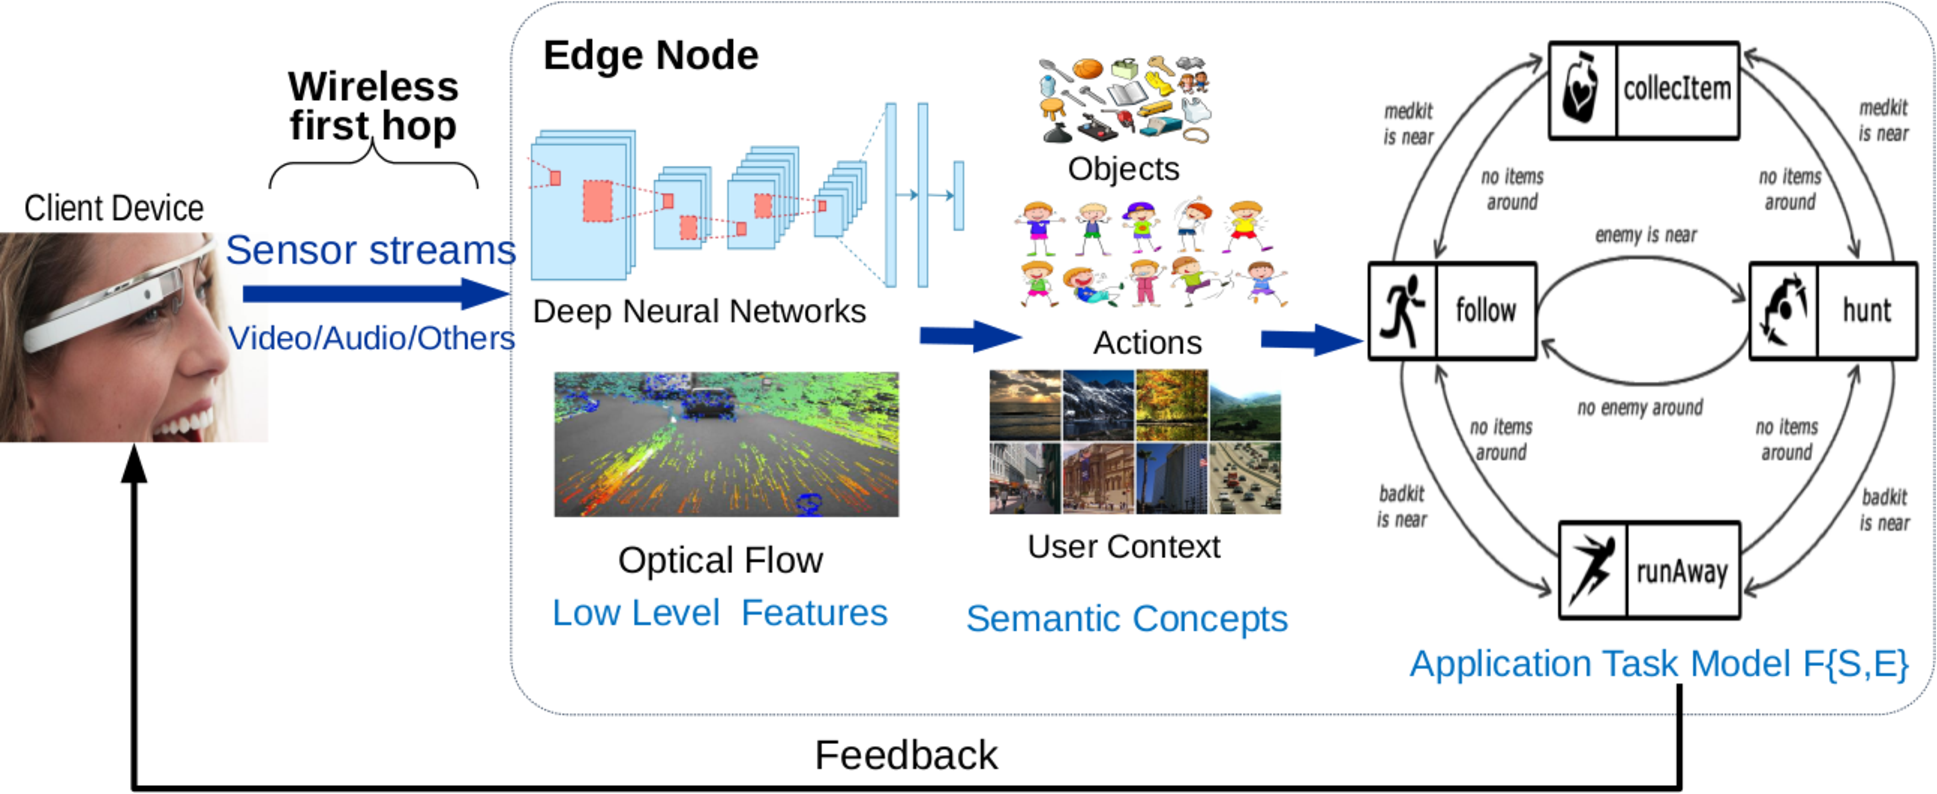
\includegraphics[width=.9\textwidth]{img/app_pipeline.pdf}
%         \captionof{figure}{Generic Human-in-the-loop Application Pipeline}
%         \label{fig:app-pipeline}
%     \end{minipage}%
% 	\begin{minipage}{.3\linewidth}
%     	\centering
% 		\includegraphics[width=\linewidth]{img/TraceReplay_GenArch}
%         \captionof{figure}{General architecture of the benchmarking suite.}
% 		\label{fig:TraceReplayArch}
% 	\end{minipage}
% \end{figure*}

% We furthermore argue that human-in-the-loop applications like AR potentially require costly gadgets for providing feedback to the human user. 
% Hence, this is another factor that contributes to the costs of such trials. 
% We hence strive for an approach to scalability tests of human-in-the-loop applications that can overcome these challenges while still sticking to an experimental approach in general.

%We address these challenges through an emulation approach.
%We address the discussed challenges on different levels.

To establish a reproducible and comparable workload, the first step in our methodology is to record a trace of the sensory input data while having a human user operate the target application. 
% The trace simply consists of the payload packets passed to the socket of the sensory device, which can be collected by TCP dump.
The collected data consists of the sensory inputs provided to the system at runtime, for instance, in the case of a visual application, the video feed from the camera.

To use the trace for reproducible experiments, we developed a benchmarking suite which can replay the trace to the original application, which results in the same computation to be performed on the edge as if a human was involved, while also ensuring a reproducible application execution path.
During the replay, many system level metrics can be collected, such as round-trip and processing times.
By enabling the client-side to play out the trace from a file, it becomes independent from human operation.
% For this, in particular a model of the human behavior needs to be defined and considered in the way the recorded trace is provided to the backend compute process. 

%\subsection{User Model}

In order to imitate a human behavior as close as possible, we propose the following user model as shown in Figure~\ref{fig:usermodel}.
We assume a user that is patient and does not make mistakes; any error message received from the application backend is ignored. We first divide a trace into steps that corresponds to individual events that should trigger feedback. If a positive feedback is received from the application, we jump ahead in the trace to replay the next step as if a human user reacts to the feedback. 
On the other hand, whenever the end of the current step is reached without having received any \emph{positive} feedback, the step is rewound a number $\tau$ of seconds.
To avoid infinite loops, where the application is stuck on a step forever, we have a maximum number of possible rewinds, after which the application shuts down.

\begin{figure}
    % Define block styles
    %         \tikzstyle{block} = [circle, draw, fill=red!20, 
    %         text width=5em, text centered, rounded corners, minimum size=4em]
    %         \tikzstyle{decision} = [diamond, aspect=2, draw, fill=yellow!20,
    %         text width=5em, text centered, rounded corners, minimum size=4em]
    %        \tikzstyle{line} = [draw, -{Latex[length=3mm]}]
    \centering
    \adjustbox{scale=0.75}{
        \begin{tikzpicture}[align=center,
        node distance=.5cm and 1.5cm,
        every initial by arrow/.style={-{Latex[length=2mm]}}]
        % Place nodes              
        \node [initial, state, minimum size=6em, initial text=] (play) {Play};               
        \node [state, above right=of play, minimum size=6em] (change) {Change\\step};
        \node [state, below right=of play, minimum size=6em] (rewind) {Rewind};
        \node [state, accepting, above right=of rewind, minimum size=6em] (shutdown) {Shutdown};
        
        
        
        % Draw edges
        \path[draw, -{Latex[length=2mm]}]
        (play) edge [bend right=20] node[left] {Step done} (rewind)
        edge [bend left=20] node[left] {Got feedback\\(\emph{positive})} (change)
        edge [out=140,in=220,looseness=6] node[left] {Step\\not done} (play)
        
        (change) edge [bend left=20] node[right] {Step changed} (play)
        edge [bend left=20] node[right] {All steps done} (shutdown)
        
        (rewind) edge [bend right=20] node[right] {Rewound} (play)
        edge [bend right=20] node[right] {Too many rewinds} (shutdown);
        
        \end{tikzpicture}
    }
    \caption{State diagram of the user model}
    \label{fig:usermodel}
\end{figure}

%A state diagram for the behavior of this user can be seen in Figure \ref{fig:usermodel}.

% Finally, by enabling this benchmark suite to run on commodity-of-the-shelf hardware, in our example we implemented the suite as an Android app, costs can furthermore be reduced by avoiding expensive gadgets to be available. 
% The suite is also based on a well-established cognitive assistance application framework, \emph{Gabriel} \cite{Chen:EarlyImplementation,Ha:TowardsWearableCogAssist}, which we believe will further aid in its adoption.

% In the following, we discuss the architecture and implementation of our benchmarking suite in more detail in particular with respect to wearable cognitive assistance applications.
% However, we stress that our methodology and in fact also our benchmark suite is applicable to most human-in-the-loop application as long as the backend code is available and the sensory input data can be captured.
% \footnote{We plan to make the benchmarking suite available to the community as Free and Open Source Software. Additionally, we plan to release the recorded traces under a Creative Commons License.}

\subsection{Architecture}

The suite has three elements, as shown in Figure~\ref{fig:TraceReplayArch}:
% the \emph{application backend}, the \emph{client emulator}, and the \emph{control backend} or \emph{server}, which interact in the following ways:

\begin{description}[labelindent=\parindent, listparindent=\parindent, style=unboxed, leftmargin=0cm]
  \item [The application backend] consists of instances of the target application running on Docker containers. 
  These correspond to real, unaltered instances of said cognitive assistance applications -- we do not model or emulate them in any way -- and they are containerized in order to be able to execute an arbitrary number of them on the same cloudlet.
  \item [The client emulator] consists of an Android application which emulates the behavior of a user operating the target cognitive assistance application while following the previously discussed user model.
  This Android app replays the previously recorded sensory data over the network to a specific \emph{application backend}, while collecting statistics and measurements of the system status. 
  %{\color{blue} Junjue: Should there be an application client in the picture? Logically, the benchmark android app feeds the application client the sensory information it needs, almost like hijacking the camera stream.}
  \item [The control backend] also runs on the cloudlet, although it could be executed in a separate cloud or cloudlet. It controls the execution of the experiments, by controlling the \emph{client emulators} over the network, initializing the \emph{application backends} and finally aggregating collected data when the experiments are completed. 
\end{description}

\begin{figure}
  \centering
  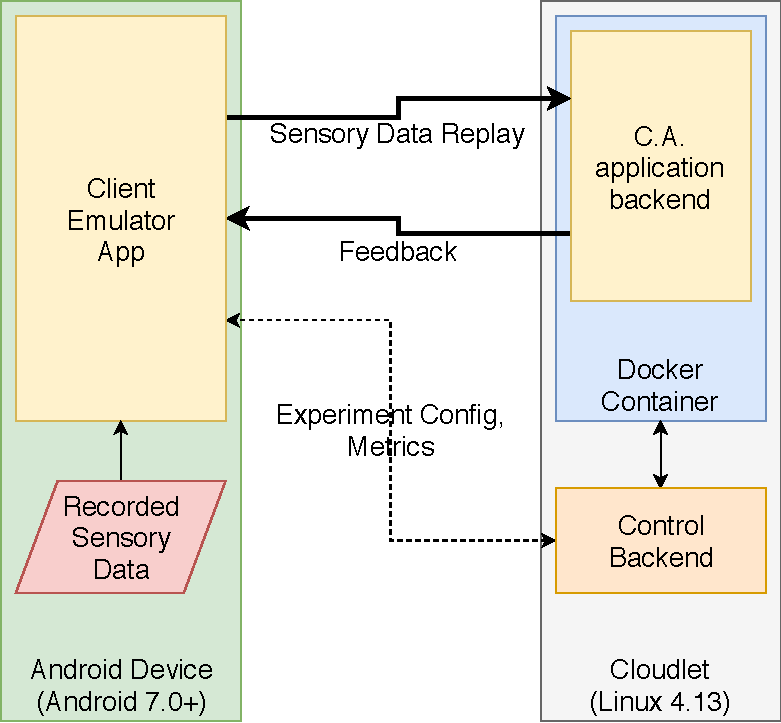
\includegraphics[width=.7\columnwidth]{publications/2018DemoScalingOnTheEdge/img/TraceReplay_GenArch}
  \captionof{figure}{General architecture of the benchmarking suite.}
  \label{fig:TraceReplayArch}
\end{figure}

\section{Demo Overview}

We will demonstrate the benchmarking framework using the \emph{LEGO Task Guidance} application previously developed by \textcite{Chen2015Early}.
This application guides a user step by step in the assembly of a LEGO model; input consists exclusively of video feed of the current state of the assembly, whereas feedback includes visual and auditory components in the form of animations and speech, respectively.

The benchmarking tool will be employed to extract key real-time metrics from this application, \emph{e.g.} average computation and network times, as well as the estimated \emph{user experience} level of the system as a whole (\emph{flawless}, \emph{impaired} or \emph{unusable}, based on the categorization in \cite{Chen2017Empirical}).

\section{Discussion and Future Work}

Some open questions and challenges remain to be tackled in the design and development of the presented tool.
To start with, the benchmarking suite is relatively narrow in the types of applications it can be applied to, currently only targeting event based cognitive assistance applications.
The tool needs to be extended to work on a much a broader spectrum of applications, in particular those that do not have a clear task model.
Furthermore, the current implementation does not support hardware accelerators (e.g. \acsp*{GPU}) that are commonly used for \ac{DNN} inference.

In addition, our current user model is simplistic. 
This model could be expanded to emulate a human user more accurately and realistically, e.g. making mistakes and responding to feedback to correct them.

We plan to extend our work in two directions. First, in addition to emulating user behaviors, we plan to simulate all the components in the system in order to generate reproducible experiments, test individual components of a real system, and identify performance bottlenecks when many users are using an application concurrently. Second, we are going to develop a statistical characterization of the application footprint, based on the data obtained from the tool.

\thesispaper{EdgeDroid}{Olguin:EdgeDroid2019}

\begin{abstract}
    %Benchmarking human-in-the-loop applications is complex.
%This limits reproducibility as well as feasibility of performance evaluations.
%In this paper we present EdgeDroid, a benchmarking suite that addresses these challenges.
%Our core idea rests on recording traces of these applications \jjw{-> application traces} which are then replayed out \jjw{remove out} in a controlled fashion based on an underlying model of human behavior \jjw{-> emulating human behaviors}.
%The traces are then exposed to the original backend compute process of the respective human-in-the-loop application, generating realistic feedback.
%This allows for an automated system that greatly simplifies benchmarking large scale scenarios.
%Our results confirm the utility of EdgeDroid as a tool for system designers, application developers and researchers.

%\jjw{Alternative version:
Many emerging mobile applications, including \acs{AR} and \acs{WCA}, aim to provide seamless user interaction.
However, the complexity of benchmarking these human-in-the-loop applications limits reproducibility and makes performance evaluation difficult.
In this paper, we present EdgeDroid, a benchmarking suite designed to reproducibly evaluate these applications.

Our core idea rests on recording traces of user interaction, which are then replayed at benchmarking time in a controlled fashion based on an underlying model of human behavior. 
This allows for an automated system that greatly simplifies benchmarking large scale scenarios and stress testing the application.
Our results show the benefits of EdgeDroid as a tool for both system designers and application developers.
%}

\end{abstract}
\section{Introduction}\label{paper:olguinmunoz2019edgedroid:sec:intro}

There is increasing interest from academia and industry in novel applications such as immersive \gls{AR} or \gls{WCA}~\cite{chatzopoulos2017hyperion,ha2014towards}, also known as human-in-the-loop applications.
These applications aim to seamlessly integrate into the lives of users to provide real-time, context-aware information by capturing user and environment information and leveraging compute-intensive algorithms to analyze the data in order to provide real-time feedback to the user.
Sensory input, such as video, audio, and other user-related data such as orientation and movement, are examples of what is typically captured, while the backend generally employs machine learning technologies such as \glspl{DNN}~\cite{ha2014towards}.
\Cref{paper:olguinmunoz2019edgedroid:fig:pipeline2} depicts such a system.
These applications are highly latency sensitive, measuring latency as the time from the capture of the sensory information until feedback is received.
Delays above a certain threshold can hurt the user experience or even make the application unusable~\cite{chen2017empirical}.

In literature, these challenging latency requirements have so far mainly been addressed through research on the optimal placement of the compute process.
There is a broad understanding today that with the advent of edge computing, human-in-the-loop applications will become viable~\cite{bittmann2017edge,flinn2012cyber,chen2017empirical,ha2013just}.
However, with respect to end-to-end latency, there are many more trade-offs involved than merely the question of where the compute backend is placed.
A human-in-the-loop application consists of various processing steps that can be influenced during the development of the application.
What kind of compression to apply to the sensory input on the uplink; which backend algorithms to utilize; how to stage the backend; when to send feedback to the human users; and how to manage congestion on the loop, as well as wireless channel fluctuations --- all these design choices impact the latency of the application.
There are also many design choices in the infrastructure: how is the sensory input conveyed to the point of computation (i.e.\ by which wireless system; with which transmission/prioritization scheme); which hardware is running at the backend; which operating system; how is the feedback conveyed back to the human user?
Finally, in production use these applications will most likely run concurrently with others.
How does this, together with other best-effort applications, impact the latencies perceived by the human user?
Existing studies~\cite{ha2014towards,chen2015early,satyanarayanan2009case,chatzopoulos2017hyperion} of this class of applications have only lightly touched upon these issues~\cite{chen2017empirical}.
On the other hand, recently published models for end-to-end latency of edge computing architectures~\cite{al_zubaidy2015performance,schiessl2017finite} are quite complex, while not accounting for the specifics of human-in-the-loop applications.
We only have a coarse understanding of the many degrees of freedom upon which end-to-end latency depends.

The goal of this paper is to provide a methodological approach to studying these latency trade-offs, along with a tool, EdgeDroid 1.0\footnote{We plan to make the EdgeDroid 1.0 benchmarking suite available as Free and Open Source Software and the recorded traces under a Creative Commons License.}, that simplifies the benchmarking of human-in-the-loop applications.
We view EdgeDroid 1.0 to be the very first, and simplest, of a family of tools that will embody increasingly sophisticated and accurate models of user behavior.

Due to the complex nature of the applications and the infrastructure, we opt for experimentally studying the trade-offs in a repeatable and controllable fashion.
This is difficult mainly due to the unpredictable reaction of human users to the feedback from the backend --- a user might very well misinterpret the feedback handed to them.
EdgeDroid 1.0 mimics the operation of human-in-the-loop applications by replaying recorded traces of sensory input.
This sensory information is then processed by the original compute process at the backend, generating feedback.
However, this feedback is not processed by humans, but by a parameterizable model of human reaction.
Through synchronized time tracking at the different processing points of the application, EdgeDroid 1.0 allows for accurate measurements of key performance metrics such as the distribution of delays across the application pipeline.
Analysis of these metrics can be performed down to the individual input sample, allowing us to zoom into the internal model of the application under consideration.
Thus, EdgeDroid 1.0 allows us to illuminate the many latency trade-offs existing at the level of the infrastructure, as well as the level of the application.
It can also be used for debugging and validation, by comparing the expected execution flow of a particular trace with the actual flow during the benchmarking.
To the best of our knowledge, this experimentally-driven benchmarking approach is the first one towards experimental performance characterization and potential optimization of human-in-the-loop applications

The rest of the paper is structured as follows:
\cref{paper:olguinmunoz2019edgedroid:sec:background} presents some background on human-in-the-loop applications.
\cref{paper:olguinmunoz2019edgedroid:sec:approach} discusses the general approach taken with EdgeDroid, while \cref{paper:olguinmunoz2019edgedroid:sec:implementation} exposes the implementation details for EdgeDroid 1.0.
We show the value of the tool through use case analysis in \Cref{paper:olguinmunoz2019edgedroid:sec:usecases,paper:olguinmunoz2019edgedroid:sec:results}, before discussing future work and concluding in \cref{paper:olguinmunoz2019edgedroid:sec:conclusions}.


%\section{Design \& Implementation}\label{sec:design_impl}
\section{Background}\label{paper:olguinmunoz2019edgedroid:sec:background}

Human-in-the-loop applications are novel applications aiming to seamlessly integrate into the lives of users and provide real-time, context-aware information.

Given the wide range of applications which fall under this concept, we have chosen to focus our initial efforts on one particular category: task-guidance \gls{WCA}~\cite{ha2014towards}.
We have chosen this type of application for two reasons: one, their relative simplicity in terms of execution flow, and two, the already well-established existing body of work~\cite{ha2014towards,chen2015early,chen2017empirical}.
Task-guidance \gls{WCA} applications aim to guide users in the execution of a task by monitoring user actions and providing real-time instructions, usually through wearable sensors and gadgets such as the Google Glass platform.
They have many potential use cases including training and assistance for professionals performing complex tasks.
Imagine for instance a specialized technician performing field repairs on a complex piece of machinery.
A task-guidance \gls{WCA} application could offer real-time guidance in this task, by analyzing a real-time video feed from the technician's head-mounted camera and providing step-by-step repair instructions.

Broadly speaking, task-guidance \gls{WCA} applications (and human-in-the-loop in general) process a multitude of inputs in parallel, which are also usually continuous, multidimensional and time-sensitive, e.g.\ video and audio feeds.
These inputs are passed to the computation backend, where they are processed in the pipeline depicted in \cref{paper:olguinmunoz2019edgedroid:fig:pipeline2}.
The first step of the backend processing is detection, which acts as a filter for irrelevant inputs.
For example, this step could consist of a computer vision detector which discards all frames for which the relevant features were not detected or which were below a set threshold.
%Given the often complex nature of the inputs, this stage usually employs Machine Learning to process them.
The remaining inputs pass on to the symbolic representation stage, where features are extracted and parameterized for subsequent computation.
For video frames, this parametrization would usually convert the visual data into a matrix representation of the  relevant features.
This representation of the inputs then continues on to the task model, where the actual application logic resides, before finally passing through the feedback generation stage at which point human-parseable feedback is generated; for instance, animations and voice commands.

\begin{figure}[b]
    \centering
    \adjustbox{scale=0.65}{
        \ttfamily\centering%\fbox{%
        \begin{tikzpicture}[align=center,
                        node distance=0.7cm and 0.7cm,
                        every initial by arrow/.style={draw=none, minimum size=0em},
                        %node styles:
                        block_center/.style ={rectangle, draw=black, thick, fill=white,
                                        text width=8em, text centered, minimum height=4em},
                        block_left/.style ={rectangle, draw=black, thick, fill=white,
                                        text width=16em, text ragged, minimum height=4em, inner sep=6pt},
                        block_noborder/.style ={rectangle, draw=none, thick, fill=none,
                                        text width=18em, text centered, minimum height=1em},
                        block_assign/.style ={rectangle, draw=black, thick, fill=white,
                                        text width=18em, text ragged, minimum height=3em, inner sep=6pt},
                        block_lost/.style ={rectangle, draw=black, thick, fill=white,
                                        text width=16em, text ragged, minimum height=3em, inner sep=6pt},
                        block_rounded/.style ={rectangle, draw=black, thick, fill=white,
                                        text width=8em, text centered, rounded corners=.55cm, minimum height=4em},
                        line/.style ={draw, thick, -{Latex[length=3mm]}, shorten >=0pt}
                ]

                \matrix [column sep=5mm,row sep=3mm] (top) {
                        \node [block_center] (detect) {Detection};
                         & \node [block_center] (repr) {Symbolic\\Repr.};
                         & \node [block_center] (model) {Task Model\\$M\{S, E\}$};
                         & \node [block_center] (feedback) {Feedback\\Generation}; \\[3ex]
                };

                \matrix [column sep=13mm,row sep=3mm, below=of top] (bottom) {
                        \node [block_rounded] (sensors) {On-body\\Sensors};
                         %& \node [block_rounded] (user) {Human User};
                         %&\node[cloud, draw, black, text centered, cloud ignores aspect=false] (user) {Human User};
                         & \node[maninblack, minimum height=5em] (user) {\Large Human User};
                         & \node [block_rounded] (hud) {HUD, Speakers,\\etc.}; \\
                };

                %\Smiley[1, below of=bottom] (smiley);


                \begin{scope}[every path/.style=line]
                        \path (detect) -- (repr);
                        \path (repr) -- (model);
                        \path (model) -- (feedback);
                        \path (feedback) -- (hud);
                        \path (hud) -- (user);
                        \path (user) -- (sensors);
                        \path (sensors) -- (detect);
                \end{scope}

                % % Place nodes       
                % \node [initial, state, draw=none, initial text=, minimum size=0em] (input) {};
                % \node [state, right=1cmof input, minimum size=7em] (detect) {Detection};
                % \node [state, right=2cm of detect, minimum size=7em] (symb) {Symbolic\\Repr.};
                % \node [state, right=.5cm of symb, minimum size=7em] (feedback) {Feedback\\Gen.};
                % \node [state, accepting, draw=none, right=1cm of feedback, minimum size=0em] (output1) {};
                % \node [state, accepting, draw=none, below=1.4cm of output1, minimum size=0em] (output2) {};

                % % Draw edges
                % \path[draw, -{Latex[length=3mm]}]
                % (input) edge node[above left] {Input} (detect)
                % (detect) edge node[above] {LEGO bricks\\in input} (symb)
                % (symb) edge node {} (feedback)
                % (feedback) edge node[above right] {Feedback} (output1)
                % (detect) edge [bend right=10] node[below left] {No LEGO bricks, thus no feedback} (output2) ;
        \end{tikzpicture}
}%}
    \caption{Pipeline of human-in-the-loop applications.}\label{paper:olguinmunoz2019edgedroid:fig:pipeline2}
\end{figure}

The task model of a task-guidance \gls{WCA} is a parameterized representation of the task in question and the steps required to complete it.
It can be represented as a Finite State Machine (FSM) \( M\{S, E\} \), where \(S\) is a set of states and \(E\) is a set of edges connecting these states.
Each state \(s_i \in S\) represents a configuration the application could potentially reach in an arbitrary execution, and each edge \(e_{i,j} \in E\) corresponds to the ability of the application to switch from state \(i\) to state \(j\) based on some user input.
We make a distinction between the set of \emph{steps} required to complete the task, \(S_s\), and \(S\), since the latter may also contain states which represent user mistakes in the execution of the task.
Thus, if we call the set of errors \(S_e\), we can further define \(S := S_s \cup S_e\).

\begin{figure}[tb]
    \centering
    \adjustbox{scale=0.75}{
    \ttfamily\centering%\fbox{%
    \begin{tikzpicture}[align=center,
        node distance=.5cm and 1cm,
        every initial by arrow/.style={-{Latex[length=2mm]}},
        line/.style ={draw, thick, -latex', shorten >=0pt}]
        % Place nodes       
        \node [state, minimum size=3em] (si) {\Large $s_{i}$};
        \node [state, above right=of si, minimum size=3em] (sj) {\Large $s_{j}$};
        \node [state, below right=of si, minimum size=3em] (se) {\Large $s^{e}_{k}$};

        \path[draw, -{Latex[length=2mm]}]
        (si)
        edge [out=140,in=220,looseness=6] node[left] {\emph{In:} none\\\emph{Out:} positive feedback} (si)
        edge [bend left=20] node[above left] {\emph{In:} correct action\\\emph{Out:} none} (sj)
        edge [bend left=20] node[right] {\emph{In:} incorrect action\\\emph{Out:} none} (se)

        (se)
        edge [bend left=20] node[below left] {\emph{In:} undo action\\\emph{Out:} none} (si)
        edge [out=230,in=310,looseness=6] node[below] {\emph{In:} none\\\emph{Out:} negative feedback} (se)

        (sj) edge [out=50,in=130,looseness=6] node[above] {\emph{In:} none\\\emph{Out:} positive feedback} (sj)
        ;

    \end{tikzpicture}
}%}
    \captionof{figure}{Segment of the internal task model of a linear task-guidance \acs{WCA}.}%
    \label{paper:olguinmunoz2019edgedroid:fig:taskmodel}
\end{figure}

These formalisms are exemplified in \cref{paper:olguinmunoz2019edgedroid:fig:taskmodel}, which represents an arbitrary segment of a linear task-guidance \gls{WCA} application.
\(s_{i}, s_{j} \in S\) represent sequential states in the execution of the task, with the edge \(e_{i,j}\) symbolizing the unique correct way of transitioning between them.
While in \(s_i\) and in the absence of inputs, the task model continuously provides instructions to the user on how to move to \(s_j\).
We will refer to this type of output as \emph{positive} feedback, since it guides the user forward in the execution of the task.
On the other hand, in the case of an erroneous input by the user, the task model moves to \(s^{e}_{k}\), where it will constantly provide instructions until the error is corrected and normal execution can resume.
This type of output directs the user to move backwards in the task model, and thus we will refer to it as \emph{negative} feedback.

\section{Approach of EdgeDroid}\label{paper:olguinmunoz2019edgedroid:sec:approach}

A system for benchmarking human-in-the-loop applications needs thus not only to be able to generate realistic, real-time inputs that follow the behavior of a real user but also be able to correctly react to feedback from the target application.
The design of EdgeDroid 1.0 tackles these challenges from two angles.
One, the generation of realistic inputs is delegated to a human user and provided to the suite in the form of a trace.
This ensures that the raw sensory input data is realistic.
Two, we propose the use of a \emph{user model} to adapt the replay of the trace to the task model and current system conditions.

Concretely, our proposed approach works in the following way:
\begin{enumerate}
    \item A trace of the sensory inputs for an execution of the task is recorded.
          For example, for a video-based application, this trace could consist of a recording from the point of view of a user performing the task.
          % Thanks to the user model, a single trace can be used for wildly different scenarios.
    \item This trace is \emph{manually} segmented into the logical steps which lead to the completion of the task.
          In other words for the generation of the trace the task model must be known to the human operator.
    \item The benchmarking suite is then configured to use this trace and a certain number of virtual users.
          This is done through a TOML~\cite{toml} configuration file on the backend.
    \item The benchmark is executed.
          Mobile devices are used to emulate users with wearable devices connecting to the \emph{real cloudlet} over the \emph{real network}.
          These devices replay the aforementioned trace, employing a \emph{user model} to adapt the trace to changing system conditions and navigate the task model to reach the desired system state.
          %\item The benchmarking suite finally outputs statistics and measurements once the benchmark finalizes.
\end{enumerate}

The extraction of metrics pertaining to the distribution of latencies across the application pipeline is the initial focus of EdgeDroid 1.0.
We calculate latencies by synchronizing clocks across the system components and storing timestamps at key points in the feedback loop.
These points include when input is sent and received, as well as when feedback is sent and received.
We collect raw data about each input-feedback cycle between user and cloudlet, which includes metrics on all the major steps in the feedback loop: uplink, downlink and processing time, presence of feedback, payload size, and so on.
This allows us to aggregate and obtain relevant statistics in postprocessing, such as average delays per step or distribution of average delays across the feedback loop.
We also store metadata regarding the task model with each measurement, for instance to link the state of the system with the current step being performed.

Note that this work does not directly target the \emph{motion-to-photon} latency metric.
This metric includes components such as sensing time and display time, which we do not consider.
We also do not evaluate the accuracy of the applications themselves, as we consider them to be \emph{black boxes}.
The system \emph{can} however be used to evaluate the trade-off between accuracy and performance, by comparing benchmarks performed using traces corresponding to different levels of accuracy.


\section{Implementation of EdgeDroid}\label{paper:olguinmunoz2019edgedroid:sec:implementation}

\begin{figure}[tb]
    \centering
    \includegraphics[width=.7\columnwidth]{publications/2019EdgeDroid/img/TraceReplay_GenArch}
    \caption{Architecture of the benchmarking suite.}\label{paper:olguinmunoz2019edgedroid:fig:TraceReplayArch}
\end{figure}

%In the following, we will detail the implementation of EdgeDroid 1.0.

The system architecture is composed of a \emph{cloudlet}, where one or more instances of the target application run, and one or more client devices, as pictured in \cref{paper:olguinmunoz2019edgedroid:fig:TraceReplayArch}.
These correspond to completely unaltered instances of the target application, running inside containers~\cite{docker}.
This allows the suite to extract metrics from them while remaining transparent to the application.
Here we also deploy the central component of EdgeDroid 1.0, the \emph{control backend}.

The \emph{control backend} is implemented in Python 3.6.
Its main purpose is to act as a central point of control and configuration of the experiments, as well as to aggregate results.
It controls the execution of the \emph{application instances} and configures the experiment and client devices, while also collecting system metrics during the execution of the benchmarks.
The experiments are configured in a centralized manner to simplify scaling.
Backend and clients communicate over TCP, using a simple application-layer protocol which allows for remote configuration, transmission of the trace data and result data, and synchronization of clocks across the system.
Note that although in the current implementation of the system the backend runs co-located with the \emph{application instances} on the cloudlet, we plan on implementing functionality for distributed monitoring from a separate computer and/or across multiple cloudlets.

The \emph{client emulators} correspond to Android applications with the main purpose of emulating a real user utilizing the target cognitive assistance application.
The emulators achieve this by mimicking the operation of real clients, but instead of obtaining the input data from the on-board sensors, they extract it from the previously recorded trace.
They replay this data over the network to the \emph{application instances} employing, as mentioned in \cref{paper:olguinmunoz2019edgedroid:sec:background}, a \emph{user model}, while simultaneously collecting client-side statistics and measurements.

The \emph{client emulators} are remote-controlled --- no interaction with a user is necessary once the application is initialized, simplifying large scale scenarios.

For our initial iteration of the EdgeDroid 1.0 benchmarking suite, we implement a preliminary user model, depicted in \cref{paper:olguinmunoz2019edgedroid:fig:usermodel}, to run on the \emph{client emulators}, designed with a linear task model in mind.
In EdgeDroid 1.0, our model is that of a user who is totally impervious to poor system performance, and suffers no annoyance, fatigue, frustration, nausea or other shortcomings of real human users.
This leads to a model of a user who responds in a precisely reproducible and deterministic manner to the same system stimulus every time.
In the future, we envision building upon this approach with many more human-like user models that more accurately emulate attributes such as fatigue and annoyance.

Each \emph{step} (i.e.\ segment) of the trace is played out to the backend until \emph{feedback} is received. If no feedback is received before the end of the step, it is replayed a pre-configured numbered of times before completely aborting the task (i.e.\ giving up).
Note that this model makes no distinction between positive and negative feedback, as both simply require the user to perform a specific action which is included in the trace.


\begin{figure}[tb]
    \centering
    \adjustbox{scale=0.7}{
    \ttfamily\centering%\fbox{%
    \begin{tikzpicture}[align=center,
        node distance=.5cm and 1.5cm,
        every initial by arrow/.style={-{Latex[length=2mm]}}]
        % Place nodes              
        \node [initial, state, minimum size=5em, initial text=] (play) {\textbf{Play}};
        \node [state, above right=of play, minimum size=5em] (change) {\textbf{Change}\\\textbf{step}};
        \node [state, below right=of play, minimum size=5em] (rewind) {\textbf{Rewind}};
        \node [state, accepting, above right=of rewind, minimum size=5em] (shutdown) {\textbf{Shut}\\\textbf{down}};

        % Draw edges
        \path[draw, -{Latex[length=2mm]}]
        (play) edge [out=270, in=180] node[below left] {Finished step but\\no feedback received} (rewind)
        edge [out=90, in=180] node[above left] {Received feedback} (change)
        edge [out=140, in=220,looseness=6] node[left] {Step\\not finished} (play)

        (change) edge [bend left=5] node[below right] {Step changed} (play)
        edge [out=0, in=90] node[above right] {All steps\\finished} (shutdown)

        (rewind) edge [bend right=5] node[above right] {Rewound} (play)
        edge [out=0, in=270] node[below right] {Too many\\rewinds} (shutdown);

    \end{tikzpicture}
}%}
    \captionof{figure}{Preliminary user model.}\label{paper:olguinmunoz2019edgedroid:fig:usermodel}
\end{figure}

\section{Use Cases}\label{paper:olguinmunoz2019edgedroid:sec:usecases}

\begin{table}[tb]
    \centering%
    \small%\ttfamily%
    \caption{Hardware used in the experiments.}%
    \label{paper:olguinmunoz2019edgedroid:tbl:cloudletclienthardware}%
    \begin{tabular}{@{}l@{\qquad}lclcl@{}}
        \toprule
         & \textbf{CPU}
         & \makecell{\textbf{Freq.}\\\textbf{[\si{\giga\hertz}]}}
         & \textbf{Cores}
         & \makecell[c]{\textbf{RAM}\\\textbf{[\si{\giga\byte}]}}
         & \makecell{\textbf{Operating}\\\textbf{System}}                                               \\
        \midrule
        \textbf{Cloudlet}
         & \makecell[bl]{Intel{\textregistered}\ Core{\texttrademark}\\i7--6700}
         & 3.4
         & 4
         & 32
         & \makecell[bl]{Ubuntu 17.10,\\kernel v4.13.0}                             \\
        \textbf{Clients}
         & \makecell[bl]{ARM{\textregistered}\\Cortex{\texttrademark}--A53}
         & 1.3
         & 4
         & 2
         & Android 7.0                                                             \\
        \bottomrule
    \end{tabular}%
\end{table}


In this section, we demonstrate the practical utility of EdgeDroid 1.0 through scalability measurements of real cognitive assistance application running on a cloudlet.
The questions we aim to answer relate to the ability of EdgeDroid 1.0 to provide relevant and accurate metrics on the performance of human-in-the-loop applications running on edge computing infrastructure.

Of particular interest is the ability to provide information about scaling limits in terms of latencies at both micro and macro levels.
We envision for instance a system designer performing the set of experiments detailed in this section.
The presented results would allow them to identify a bottleneck in performance.
From that they could extrapolate to how they need to scale their system hardware to manage their expected load, or they might conclude that their wireless link is not good enough for the average case.
They can also obtain real-time measurements to determine runtime measures to optimize performance, such as load balancing.
On the other hand, imagine an application developer who wishes to optimize their application.
EdgeDroid 1.0 would allow them to extract valuable information on where to focus their efforts.

%\todo[inline]{Also keep in mind that a perhaps more important question relates to on-line application optimization. Think about measures that can be applied at run-time on the side of the infrastructure to improve application performance - this is what one would like to explore here in this section.}

We chose the open source \emph{Gabriel} platform~\cite{ha2014towards} running the LEGO assistance application~\cite{chen2017empirical} for our experimentation.
This application guides a user through the assembly of a 2-dimensional LEGO model with visual and auditory instructions.
This functionality can be observed online.\footnote{\url{https://www.youtube.com/watch?v=7L9U-n29abg}}
We chose it due to its maturity and stability compared to other applications which run on the \emph{Gabriel} platform, as well as the relative simplicity of the task it performs.
The application employs a straightforward, linear task model as the one described in \cref{paper:olguinmunoz2019edgedroid:sec:background}.
Each state only allows for one specific correct action by the user, and any other action triggers negative feedback until the application is reset to the previous state.
The application has several different LEGO models to choose from, all of them roughly equal in complexity.
The specific task chosen for the experiments detailed in this section consists of the assembly of a 7-piece LEGO model.
The task has 7 distinct steps, and takes an average of approximately 2 minutes for a normal, untrained user to perform.
The input to the task model consist of a video stream captured either by an Android phone or a Google Glass wearable.

It should be noted that the \emph{Gabriel} platform by design always sends an acknowledgment for each input it receives, even when it is discarded, allowing us to measure latency for all inputs.


\cref{paper:olguinmunoz2019edgedroid:tbl:cloudletclienthardware} shows the hardware and software specifications for the cloudlet and the clients.
The components communicated through a single consumer-grade WiFi (IEEE 802.11n, \SI{2.4}{\giga\hertz}) access point.
We considered exclusively off-the-shelves hardware and software.
To minimize interference during the measurements, we locked the wireless link to the least congested available channel.
%Intel\textregistered \@ TurboBoost\texttrademark \@ technology was activated on the cloudlet CPU and the frequency of all cores locked to \SI{3.7}{\giga\hertz} to ensure consistency across experiments.

To ensure statistical independence between each emulated user, the initialization of each client emulator was subject to a random delay within a predefined window of time at the beginning of each run.
This way, the time between the start of any two clients in any repetition of the experiment is stochastic, leading to independent samples from each.
We also only take into account metrics collected while \emph{all} clients were concurrently running.

Our measurements were obtained from series of scenarios, repeated 100 times each.
We performed three \emph{optimal} scenarios with 1, 5 and 10 clients each, the signal strength of the WiFi link being an excellent \SI{-40}{\dBm}.
Next, a scenario where the 10 clients were moved to another room roughly \SI{10}{\meter} away, thus degrading the network link to an average measured strength of \SI{-73}{\dBm}.
Finally, we studied an additional optimal single-client scenario focused on latency distributions and jitters within application execution path.
This scenario is used to showcase the utility of EdgeDroid 1.0 for application developers.

\section{Results}\label{paper:olguinmunoz2019edgedroid:sec:results}

\begin{figure}
    \centering%
    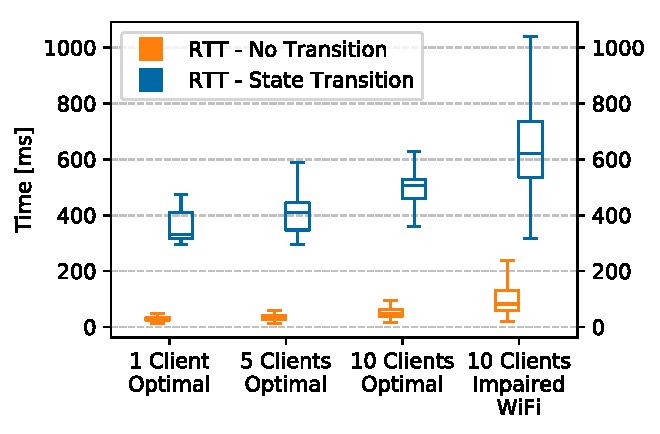
\includegraphics[width=.85\columnwidth]{publications/2019EdgeDroid/plots/comparison/nofonts/rtt_fb_vs_nofb}%
    \caption{Comparison of round-trip-times for inputs that triggered a state transition in the task model versus inputs that did not.}%
    \label{paper:olguinmunoz2019edgedroid:fig:comparison:rtt}%
\end{figure}%
\begin{figure}
    \centering%
    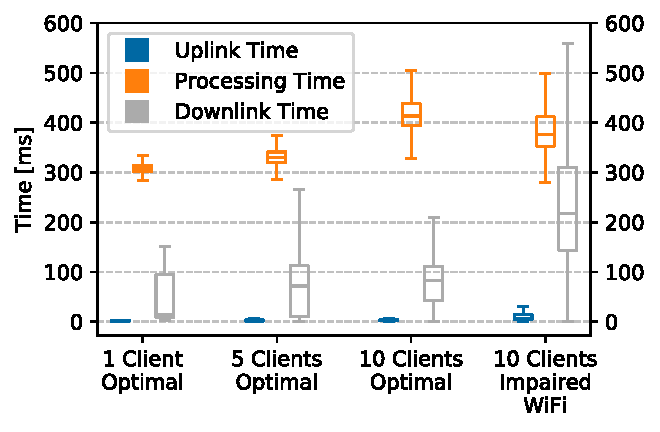
\includegraphics[width=.85\columnwidth]{publications/2019EdgeDroid/plots/comparison/nofonts/box_feedback}%
    \caption{Distribution of latency across system components for inputs that triggered a state transition in the task model.}%
    \label{paper:olguinmunoz2019edgedroid:fig:comparison:feedback}%
\end{figure}%
\begin{figure}%
    \centering%
    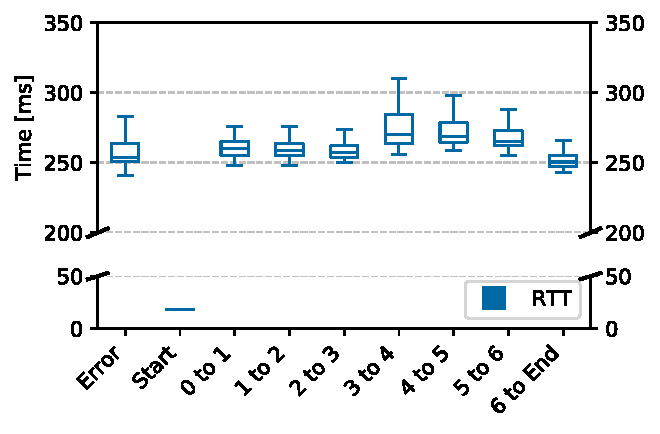
\includegraphics[width=.85\columnwidth]{publications/2019EdgeDroid/plots/comparison/nofonts/box_taskstep}%
    \caption{Round-trip-times for input-feedback cycles associated with state transitions in the internal task model for a single client connected over an optimal wireless link.}%
    \label{paper:olguinmunoz2019edgedroid:fig:comparison:tasksteps}
\end{figure}%

%In \cref{fig:comparison:feedback,fig:comparison:rtt,fig:comparison:tasksteps} we show some of the results obtained from the use case scenarios.
The results presented in this section provide valuable insights on both the system limits as well as on the application itself.

\cref{paper:olguinmunoz2019edgedroid:fig:comparison:rtt} presents a comparison of the total measured round-trip-times (RTTs) both for inputs which caused a state transition and inputs that did not.
Next, \cref{paper:olguinmunoz2019edgedroid:fig:comparison:feedback} shows a comparison of the distribution of latencies across system components for inputs that caused an internal state change in the task model of the application.
We differentiate according to the three main components contributing to latency, namely \emph{uplink} and \emph{downlink transmissions}, and \emph{backend processing}.
Finally, \cref{paper:olguinmunoz2019edgedroid:fig:comparison:tasksteps} depicts the distribution of RTTs for each transition in the internal task model for a single client connected over an optimal wireless link.
These metrics were calculated by recording the measured input-feedback cycle delay corresponding to a change in state within the application.
Thus, for instance, the measurements located at column ``3 to 4'' in the figure correspond to the aggregated round-trip-times for every input-feedback cycle corresponding to a change from state 3 to state 4 within the application task model, for the 100 repetitions of the scenario.

In the following discussion we will refer to inputs which triggered a transition in the task model as \emph{feedback-rich inputs} and those that did not as \emph{feedback-less inputs}.

For the analysis of these results, we will take into consideration the bound of \SI{600}{\milli\second} response time for step-by-step task-guidance derived by the authors of~\cite{chen2017empirical}.
This bound marks the point after which further delays in the delivery of feedback to the user start to negatively affect user experience, and allows for a straightforward evaluation of the responsiveness of the system.

We will begin our analysis of the experiment results with \cref{paper:olguinmunoz2019edgedroid:fig:comparison:rtt}.
These results present a stark contrast in the round-trip-times for inputs which cause a state transition versus inputs that do not, with RTTs for the former being up to an order of magnitude greater.
It's worth mentioning though that responses to feedback-less inputs are invisible to the user, and are just included here as a sort of baseline to compare feedback-rich round-trip times with.

We can identify a pair of interesting effects in the scaling of the task-guidance \gls{WCA} application.
One, scaling behavior for the application seems to be linear with respect to the number of clients.
Two, in the case of the impaired WiFi, the effect on the feedback-rich inputs is very pronounced, with the average of the RTTs for these inputs being over the previously discussed bound of \SI{600}{\milli\second}.

It is worth noting that already at just 10 clients the response times for feedback-rich inputs are very close to the bound.
Looking at this through the lens of a an application developer, it could hint at a need for optimization of the later parts of the application pipeline, since RTTs for inputs which are discarded in the detection stage of the pipeline (i.e.\ feedback-less inputs) are still well below \SI{200}{\milli\second}.

EdgeDroid 1.0 allows researchers to zoom into specific components of the application feedback loop, as exemplified by \cref{paper:olguinmunoz2019edgedroid:fig:comparison:feedback}.
From this figure it is clear that the main component which contributes to latency in the optimal case is the backend processing, further lending credibility to our previous comment on the need for optimization.
Nevertheless, when the link quality decreases, the delays on the downlink start to overshadow the delays on the processing.
Here, the downlink time sometimes almost reaches the ideal bound by itself.
A system designer might then conclude from this that in order to be able to scale the application, their focus needs to be on improving the quality of the wireless link before increasing the processing power on the backend.

Finally, EdgeDroid 1.0 allows even more insights to be gained by homing in to individual steps in a task-guidance \gls{WCA}. Consider \cref{paper:olguinmunoz2019edgedroid:fig:comparison:tasksteps}.
The figure shows clears spikes in latencies at the transitions from task state 3 to 4 and from task state 4 to 5, which could indicate to the application developer that these specific transitions are ripe for optimization.

\section{Conclusions \& Future Work}\label{paper:olguinmunoz2019edgedroid:sec:conclusions}

Benchmarking human-in-the-loop applications is hard, given their tight interaction with human users who complicate the scaling and repeatability of experiments.
In this paper, we have presented a benchmarking suite for this type of applications, called EdgeDroid 1.0, capable of cutting out the need for users in performance evaluations.
We achieve this by employing pre-recorded sensory input traces which we play over the network to the real application backend, employing a parameterized user model to react to feedback.
We demonstrate its utility through a series of use case scenarios, from which we are able to extract metrics regarding latency both in regards to the application itself and the hardware stack.
We believe the EdgeDroid 1.0 suite thus represents an important first step towards enabling inexpensive and low-complexity large-scale research on the scaling limits of this type of applications, a requirement for wide adoption of the technology.

Nonetheless, there is still future work to be done.

The user model presented in this paper is only preliminary, and we are currently conducting research in characterizing user behavior when interacting with \gls{WCA} applications in order to present a more complete model in the future.
As mentioned in \cref{paper:olguinmunoz2019edgedroid:sec:implementation}, in EdgeDroid 1.0, our model is that of a user who does not suffer any of the shortcomings of real human users such as annoyance, fatigue, frustration, nausea.
Rather, EdgeDroid 1.0 models a perfectly stoic user who is like an automaton and responds in a precisely reproducible and deterministic manner to the same system stimulus every time.
Of course, no real human user is an automaton.
In the future, we envision creating  many versions of EdgeDroid (i.e., EdgeDroid 2.0, EdgeDroid 3.0, etc.) that embody more human-like user models that more accurately emulate attributes such as those mentioned above.
Experimental validation of these human-like user models via user studies will be an important part of our future work.

We are also working on expanding the benchmarking suite to also work first with other types of Wearable Cognitive Assistance, and later with other categories of human-in-the-loop applications.
Other types of \glspl{WCA} we will consider in future iterations of the tool include real-time task-assistance \gls{WCA} applications (such as the Ping-Pong application described in~\cite{chen2017empirical}), which don't have a linear task model like task-guidance \gls{WCA} and have tighter latency bounds and context- and information-providing \gls{WCA} applications, for instance, applications which recognize faces and provide relevant social-media information related to that person.
The latter also do not have a linear task model, but present more lax latency bounds.

\begin{acks}
    We thank Bobby Klatzky and Dan Siewiorek for many valuable technical discussions relating to this research.
    We also thank our shepherd, Wenjun Hu, and the anonymous reviewers for helping us improve the paper.
    This research was supported in part by the \gls{NSF}, grant number \verb|CNS-1518865|, the VINNOVA grant \verb|MERIT (2017--05232)|.
    Additional support was provided by Intel,\ Vodafone,\ Deutsche~Telekom,\ Verizon,\ Crown~Castle,\ NTT,\ and the Conklin~Kistler family fund.
    Opinions, findings, conclusions or recommendations expressed in this material are those of the authors and do not necessarily reflect the view(s) of their employers or the mentioned funding sources.
\end{acks}

\thesispaper{Impact of delayed response on WCA}{Olguin:ImpactWCA2021}{PLOS}

\begin{abstract}
    \glsunset{WCA}
  Wearable Cognitive Assistants (\gls{WCA}) are anticipated to become a widely-used application class, in conjunction with emerging network infrastructures like 5G that incorporate edge computing capabilities.
  While prototypical studies of such applications exist today, the relationship between infrastructure service provisioning and its implication for \gls{WCA} usability is largely unexplored despite the relevance that these applications have for future networks.

  This paper presents an experimental study assessing how \gls{WCA} users react to varying end-to-end delays induced by the application pipeline or infrastructure.
  Participants interacted directly with an instrumented task-guidance \gls{WCA} as delays were introduced into the system in a controllable fashion.
  System and task state were tracked in real time, and biometric data from wearable sensors on the participants were recorded.
  Our results show that periods of extended system delay cause users to correspondingly (and substantially) slow down in their guided task execution, an effect that persists for a time after the system returns to a more responsive state.
  Furthermore, the slow-down in task execution is correlated with a personality trait, neuroticism, associated with intolerance for time delays.
  We show that our results implicate impaired cognitive planning, as contrasted with resource depletion or emotional arousal, as the reason for slowed user task executions under system delay.
  The findings have several implications for the design and operation of \gls{WCA} applications as well as computational and communication infrastructure, and additionally for the development of performance analysis tools for \gls{WCA}.\@
\end{abstract}

\section{Introduction}

Wearable Cognitive Assistants, \gls{WCA} for short, have recently started to garner attention from the research community~\cite{ha2014towards,chen2015early}.
They represent a novel category of highly interactive and context-sensitive augmented reality applications, that aim to amplify human cognition in both day-to-day tasks and professional settings.
Their mode of operation is analogous to how \gls{GPS} navigation systems guide drivers, by seamlessly providing relevant instructions and feedback relating to the current task at hand.
Note that this implies seamless interaction with the context of the user --- at no moment does the user need to trigger an update explicitly, as the application is constantly tracking the state of the target task.
An example is an IKEA Assistant~\cite{IKEAAssistant} which monitors the assembly of a piece of furniture in real time, providing timely, step-by-step feedback to guide the user toward completion.

WCA systems were originally inspired by assistive use cases for people suffering from some form of cognitive decline, either through aging or because of traumatic brain injuries~\cite{ha2014towards,satyanarayanan2019augmenting}.
More recently, they have been applied to a broader range of use cases, including step-by-step guidance on complex assembly tasks~\cite{chen2017empirical}.
Non-wearable augmented reality and cognitive assistance systems have already been proven to be valuable tools in the industrial workplace~\cite{funk2015cognitive,gorecky2011cognito}.
Detethering this assistance from its current fixed location will surely make it available to many more fields. 

Based on these use cases, we identify three main requirements for \gls{WCA}:\@
\begin{enumerate}
    \item\label{paper:olguinmunoz2021impact:item:pervasive} \gls{WCA} systems should be available whenever the user requires them, without being tethered to a particular physical location. Assistants need to be pervasive and mobile.

    \item\label{paper:olguinmunoz2021impact:item:interaction} Interaction with the system should be immersive and seamless, i.e.\ the assistant should be able to analyze the current context and automatically provide relevant feedback without explicit commands from the user.
    In this sense, \gls{WCA} is expected to operate much like a human assistant would, by observing the performance of the user and offering guidance proactively.

    \item\label{paper:olguinmunoz2021impact:item:lowlatency} Feedback should be ``quick'', relative to the task at hand.
    This requirement is further strengthened by the previously mentioned ``seamless interaction'' characteristic of these systems.
    This means that users will have expectations of constant, immediate feedback as they progress through the task.
    In the case of a step-by-step task like IKEA, delayed feedback might simply confuse or distract the user.
    However, in a highly interactive task like a \emph{Ping-Pong assistant}~\cite{PingPongAssistant,chen2015early} late guidance is at best a nuisance and at worst a severe handicap.
\end{enumerate}

\cref{paper:olguinmunoz2021impact:item:pervasive} implies use of lightweight and low-power devices, preferably a wearable device that frees both hands for work.
\cref{paper:olguinmunoz2021impact:item:interaction}, on the other hand, suggests a level of context sensitivity and proactivity that can only be provided by real-time analysis of sensor inputs such as video and audio feeds.
The compute-intensive processing suggested by \cref{paper:olguinmunoz2021impact:item:interaction} cannot be met by the lightweight wearable devices suggested by \cref{paper:olguinmunoz2021impact:item:pervasive}.
Only by offloading computation from a wearable device to cloud-based or edge-based infrastructure can this circle be squared.
However, offloading implies an extended end-to-end pipeline with many potential sources of queueing, transmission, and processing delays.
\cref{paper:olguinmunoz2021impact:item:lowlatency} therefore emerges as a key concern, requiring deep understanding of the impact of end-to-end delays on \gls{WCA} users.

% However, additional challenges remain in the path toward widespread adoption.
\cref{paper:olguinmunoz2021impact:item:lowlatency} forms the base motivation for the research presented in this paper.
We still have a very limited understanding of how humans react to delays in these systems --- specifically, how changes in system responsiveness impact users.
\emph{System responsiveness} here denotes a qualitative scale ranging from \emph{high} (that is, not subject to delay or subject to negligible delay with respect to human perception) to \emph{low} (i.e.\ subject to considerable delay).
% Conversely, QoE is understood to range from \emph{good} (i.e.\ users enjoy interacting with the application) to bad (users dislike interacting with the application).
Characterizing the relationships between system responsiveness and user behavior and quality of experience is of paramount importance for the design and evaluation of these applications.
It is generally acknowledged, for instance, that a system going from a state of high responsiveness to one of low responsiveness can cause a drop in quality of experience~\cite{dabrowski201140}.
Furthermore, this could cause users to modify the temporal paramaters of their behavior when interacting with the system, generating a sort of \emph{feedback loop} between user and system.
A clear understanding of these relationships would allow, for instance, for the development of strategies for load balancing and optimization for large-scale deployment of \gls{WCA}.\@
% Although maximizing QoE through over-engineered systems and networks would be a ``simple'' solution to this problem, in practice, the prohibitive costs of infrastructure make finding the optimal trade-off between QoE and cost a valuable endeavor.

This paper builds upon preliminary work in the field of time perception and delay characterization of \gls{WCA}.\@
We expand upon the findings of Ha et al.~\cite{ha2014towards}, who identified the need for low-latency offloading in \gls{WCA}, and of Chen et al.~\cite{chen2017empirical}, who outlined the bounds for ``noticeable'' and ``unbearable'' latencies in these systems.
While these bounds present a general understanding of when it is likely that a user will stop using an application, they do not provide any insights as to what happens \emph{before} that --- i.e.\ how human behavior changes with system responsiveness.
We aim to tackle this gap in knowledge through the characterization of human responses to delays in the application pipeline, using latencies in the range defined by the previously established bounds.
This is an important step toward a more systematic understanding of human behavior in this domain.

We present in this paper the design and elaboration of an experimental \gls{WCA} test-bed.
This test-bed was subsequently employed in a study in which undergraduate students of diverse fields of study, aged between 18 and 25 years old, were asked to interact with and follow the instructions given to them by a cognitive assistant.
Unbeknownst to the participants, we altered the responsiveness of the system in real-time and recorded the resulting behavioral and physiological reactions. 
The participants wore an array of biometric sensors measuring physiological responses that have proven useful in assessing cognitive workload during human-computer interaction~\cite{haapalainen2010psycho,kumar2016measurement} such as heart rate and \gls{EEG}.\@

Through this experimental set-up, we intended to answer four core research questions relating to human responses to decreased application responsiveness.

\begin{itemize}
  \item \emph{Do subjects change the temporal profile of their actions in relation to system latency?}

  In line with previous research in this area, we expected subjects to change their temporal profiles as system responsiveness decreased.
  The extent or form of these changes were however unknown.
  We also hypothesized that large enough drops in responsiveness could lead to complete abandonment of the task by subjects.

  Our results show an emergent pacing effect on user actions as system responsiveness is reduced.
  While it would seem self-evident that users take longer to complete a task while using a system with low responsiveness --- as they have to wait longer for new instructions --- our study found that user slow-down represents a source of substantial additional delay.
  To be more precise, the data indicate that users slow down not only because they have to wait for the system to catch up, but that their reactions to new instructions is also delayed.
  Moreover, this effect scales with the decrease in responsiveness and remains for a while, even after system responsiveness improves.
  
  \item \emph{Do subjects show signals of arousal in physiological responses to changes in system latency?}
  
  We hypothesized subjects would show signs of stress and frustration as system latency increased, due to the added annoyance of dealing with an unresponsive system.

  The results we present, however, seem to refute this hypothesis. 
  We were not able to detect any significant effects on the physiological signals obtained from the biometric sensors as sytem responsiveness was altered.
  
  \item \emph{Are responses to delay effects in subjects mediated by cognition and/or emotion?}
  
  In line with previous items, we expected delay effects in subjects to be mediated primarily by emotion.
  In particular, we expected emotional effects to be correlated with the strength of the added delay.

  The results point in a different direction though, indicating that reduced responsiveness in \gls{WCA} systems leads to a disruption of participants' cognitive plan for the task and not to an emotional response.
  This is evidenced by the previously discussed pacing effect and the lack of significant physiological responses.

  \item \emph{Are these effects mediated by personality indicators in any way?}
  
  Finally, we hypothesized that the individual trait of \emph{neuroticism}~\cite{john1999big} would play a role in mediating these effects, as it has previously been connected to intolerance for time delay~\cite{hirsh2008delay}.
  We also expected \emph{focus} and \emph{involvement}~\cite{witmer1998measuring} to play roles in this.

  The results obtained agree with our hypothesis. 
  We found significant effects of neuroticism on the responses exhibited by subjects, and all three traits were found to play a role through factor analysis.

\end{itemize}

% Our results indicate that reduced responsiveness in \gls{WCA} systems leads to a disruption of participants' cognitive plan for the task.
% This is evidenced by an emergent pacing effect on user actions as system responsiveness is reduced.
% While it would seem self-evident that users take longer to complete a task while using a system with low responsiveness --- as they have to wait longer for new instructions --- our study found that user slow-down represents a source of substantial additional delay.
% To be more precise, the data indicate that users slow down not only because they have to wait for the system to catch up, but that their reactions to new instructions is also delayed.
% Furthermore, this effect persists for a while after system response improves and is modulated by intrinsic personality traits, in particular, \emph{neuroticism}~\cite{john1999:bfi}. 

We believe that these results provide concrete and relevant implications for \gls{WCA} design, deployment, and optimization.
One example is the behavioral slow-down, as it extends application runtime significantly, and thus has clear and direct implications for resource and power consumption.
Another is the fact that the adverse effects of delay on users do not immediately subside as delay is diminished --- this has potential consequences for resource allocation strategies.
Moreover, in multi-user scenarios, the dependency of user slow-down effects on delay mean efficient resource allocation across applications potentially looks different from what could be considered ``fair''.

Our hope is that the results we provide might prove useful for the understanding and optimization of deployments of \gls{WCA}.\@
These results represent unexpected, valuable findings, which can be employed to model and understand how users interact with latency in applications and systems, and develop resource allocation and power optimization strategies.
Additionally, we hope that the results we provide might pave the way for the improvement of performance evaluation tools such as our previous work in \cite{olguinmunoz2018demoscaling,olguinmunoz2019edgedroid}.
Such systems would greatly benefit from this knowledge, as it would allow for the design and implementation of realistic models of human behavior, making highly accurate benchmarks a reality in the domain of \gls{WCA}.\@

The structure of this paper is as follows.
We describe the existing body of research around time perception and the effects of delay on human performance in \cref{paper:olguinmunoz2021impact:sec:background}.
\cref{paper:olguinmunoz2021impact:sec:experimentaldesign} presents the experimental design, measures, and specific protocol.
Then, in \cref{paper:olguinmunoz2021impact:sec:results} we detail the results of our experiment.
Implications for further modeling of the effects of delay are presented in \cref{paper:olguinmunoz2021impact:sec:discussion} before finally concluding the paper in \cref{paper:olguinmunoz2021impact:sec:conclusion}.

\section{Background and Related Work}\label{paper:olguinmunoz2021impact:sec:background}

% Overarching theo construct: people perform temp seq task in the framework of cognition and emotion and individual differences mediate response to delay. In particular we view cognition as described by models such as ACT-R as a seq of procedures.

% Section 2.
% Accordingly we review time perception...

% Our overarching theoretical construct is the idea that people perform temporally sequential tasks in the framework of cognition and emotion.
% Additionally, we hypothesize that individual diferences between subjects moderate responses to delays in the feedback during the execution of a task.
% In particular, we view cognition as described by models such as {ACT-R}~\cite{neves1981knowledge}; i.e.\ as a sequence of procedures performed by the subject.

Our overarching theoretical construct is the idea that people perform temporally sequential tasks in the framework of cognition and emotion.
In particular, we view cognition as described by models such as {ACT-R}~\cite{neves1981knowledge}; i.e.\ as a sequence of procedures performed by the subject.
Additionally, we hypothesize that individual diferences between subjects moderate responses to delays in the feedback during the execution of a task. 

Accordingly, in the following we review background work in the areas of 
\begin{inlineenum}[label={}, before=\unskip{: }, itemjoin={{; }}, itemjoin*={{; and }}]
  \item[(\cref{paper:olguinmunoz2021impact:ssec:timeperception})] time perception
  \item[(\cref{paper:olguinmunoz2021impact:ssec:potentialmechs})] mechanisms relating human performance to delay.
\end{inlineenum}

\subsection{Time perception in computing systems}\label{paper:olguinmunoz2021impact:ssec:timeperception}

The question of how people respond to delay in a computer system is grounded in how people perceive time.
Time perception has been described as regulated by an attentional gate that, when opened, starts a cognitive pulse counter~\cite{zakay1995attentional,zakay1996role}.
More recent research indicates, however, that duration perception is highly malleable and the result of multiple timing mechanisms found in overlapping, flexible neural systems~\cite{bruno2016multiple,wiener2011multiple}. 
The estimation of an event's duration varies with context of various types
\begin{inlineenum}[label={(\roman*)}, before=\unskip{: }, itemjoin={{; }}, itemjoin*={{; and }}]
    \item events subsequent to a long or short interval are contracted or extended, respectively~\cite{heron2012duration}
    \item repeated events tend to be perceived as shorter than novel ones~\cite{matthews2011stimulus}
    \item arousal can expand durations~\cite{droit_volet2011emotion}.
\end{inlineenum}

Expectations play a critical role in time perception as well~\cite{zakay1995attentional,zakay1996role}.
It has been shown that people have a general tendency to be hypersensitive to delays in worse-than-expected states, and under-sensitive to meeting or exceeding expectations~\cite{loewenstein1992anomalies}.
Accordingly, failures to meet expected fast response times tend to be experienced as highly negative, whereas fast latencies are not noticed.
Violations of expectancy have a strong impact on the acceptability of computer systems.
Users of a computer system anticipate the latency for events, for which the standards only become more stringent as systems improve in response time.
In immersive systems like \gls{WCA}, which aim to provide seamless interaction, delays are particularly noticeable.

It has long been recognized that slow system response times can undermine cognitive processing, slow the pace of users, and lead to stereotyped behavior and errors, as well as cause negative emotional consequences~\cite{dabrowski201140}.
However, standards for what constitute tolerable delays have changed dramatically compared to three decades ago, when delays on the order of \SI{10}{\second} were deemed acceptable~\cite{nielsen1994usability, shneiderman2016designing, seow2008designing}.
Today's user context, and \gls{WCA} in particular, often demand response times orders of magnitude shorter.

For \gls{WCA} the acceptable range for latencies was explored by Chen et al.~\cite{chen2017empirical}, by constructing assistants for tasks with a range of time constraints, including step-by-step tasks and more interactive contexts like playing Ping-Pong against a human opponent.
They then proposed a latency tolerance zone according to the task demands.
For an essentially self-paced task like LEGO assembly, they found two key ranges of latency; unnoticeable, \SIrange{0}{0.6}{\second}; and impaired, \SIrange{0.6}{2.7}{\second}. 
Beyond that, users could begin to show the negative outcomes previously catalogued~\cite{dabrowski201140}.


\subsection{Mechanisms Relating Delay to Human Performance}\label{paper:olguinmunoz2021impact:ssec:potentialmechs}

While behavioral changes and negative interaction outcomes have been well documented in prior research on system delay, the specific mechanisms that mediate these outcomes are less well understood. 
These mechanisms could be cognitive or emotional in origin.

A first possible explanation comes from research on cognitive and motor planning. 
Delay may move users from relatively automatic to more attention-demanding processing.
Cognitive and motor tasks are commonly described as a hierarchical system, progressing from high-level goals to the sequence of commands that accomplishes them.
As competency in a task increases, execution of the hierarchy becomes increasingly automated.
Automatization has been described from a computational perspective in {Anderson's ACT-R}~model as the compiling of multiple productions into one~\cite{neves1981knowledge}.
Neural measurements indicate that with automaticity, control moves from frontal brain areas to more posterior ones~\cite{jeon2015degree,puttemans2005changes}, and similar distinctions have been related to temporal processing~\cite{lewis2003distinct,koch2009neural,lee2019limiting}.

Although activities guided by a \gls{WCA} are not simple motor actions, immediate feedback after each of a series of repeated actions should promote development and automatic execution of a hierarchical plan.
Delays, in contrast, would disrupt such a plan through the loss of automated control~\cite{lee2019limiting}.

A second, alternative explanation of delay effects appeals to emotional systems rather than cognitive processes.
As users of a system become emotionally aroused by delay, they may be subject to generalized arousal, causing decrements in performance~\cite{lee2019limiting}.

Finally, a third potential explanation of delay effects is what has been called ``ego depletion'', the notion that expending effort on self-control eliminates resources needed for further effort~\cite{baumeister74tice,lin2020strong}.

The various processing accounts of delay effects predict different outcomes, which we will consider in the context of the current data.
If delay increases attentional demands on cognitive processes, responses should be slowed and errors expected, particularly on time-critical tasks.
Generalized arousal triggered by emotional stress from delay should emerge in physiological measures, such as increased heart rate or skin conductivity.
Arousal can also reduce movement smoothness or add erratic gestures~\cite{pijpers2003anxiety}.
Ego depletion has been found to produce premature responses culminating in error~\cite{lin2020strong}, or to lead to abandoning a task entirely~\cite{baumeister74tice}. 

Over-arching prescriptions for tolerable system response time have not tended to take into account individual differences in users with respect to salient variables like cognitive ability or personality. 
Relevant research can be found in studies of delay discounting, the tendency to devalue rewards for which one must wait.
High discounting rates, indicative of waiting intolerance, have been associated with negative social and academic outcomes.
Hirsh et al.~\cite{hirsh2008delay} found that higher discounting was associated with extraversion among those with low cognitive function, whereas lower discounting was associated with emotional stability (low neuroticism) for people with high cognitive function.
Among computer system users who tend to have relatively high cognitive ability (which presumably describes the present experimental population), this points to neuroticism as a personality factor that might modulate tolerance for waiting. Extraversion could also  be  a moderating factor among the broader target audience of \gls{WCA}, which are intended for relatively inexperienced users of an application.
These and other measures of individual variation were considered here.

\section{Experimental Design}\label{paper:olguinmunoz2021impact:sec:experimentaldesign}

The core elements of our experiment are shown in \cref{paper:olguinmunoz2021impact:fig:experimentaltestbed}:
\begin{itemize}
    \item Subjects interact with a \gls{WCA} while wearing an array of biometric sensors.
    \item The \emph{responsiveness} of the application, i.e.\ the interval of time between an input being provided to the system and the associated output returned to the user, is manipulated in real time. 
    The effects of these manipulations on the subjects are recorded and subsequently analyzed.    
\end{itemize}

\begin{figure}[h]
  \centering
  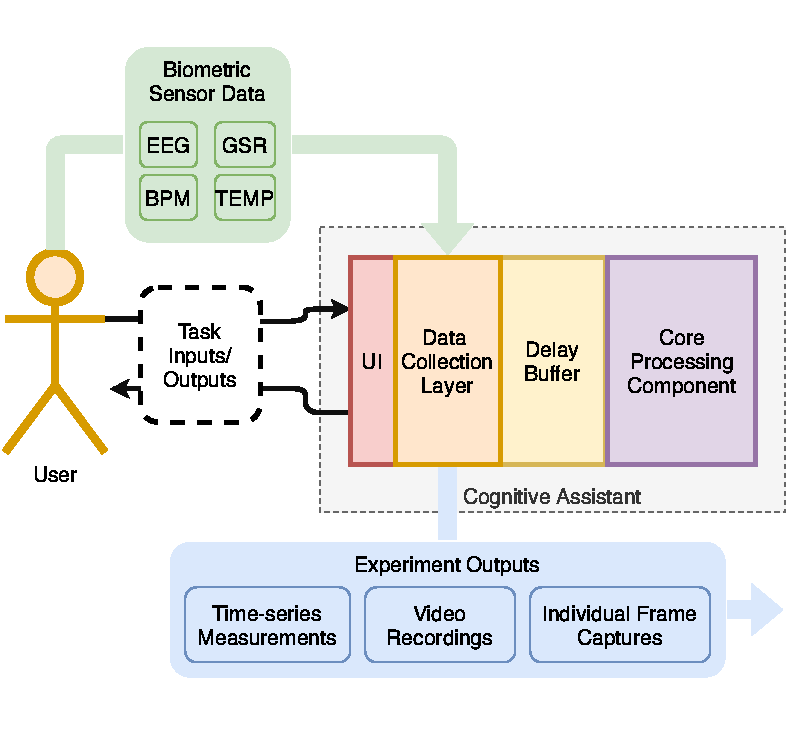
\includegraphics[width=.8\textwidth]{publications/2021ImpactDelayedResponse/Fig1.eps}
  \caption{Experimental test-bed.
  Participants interact with the cognitive assistant through task-related inputs and outputs --- in practice, these correspond to the video feed captured by the assistant and the instructions provided by it.
  The assistant itself has been instrumented with a data collection layer, which collects and processes experiment-related data such as biometric signals from the participants (these are merely processed here and do not form part of the inputs to the cognitive assistant as such, however), and a delay buffer, which introduces controlled delays in the transit of information from the core processing component.}%
  \label{paper:olguinmunoz2021impact:fig:experimentaltestbed}
\end{figure}

This study was conducted with the approval of the Carnegie Mellon University Institutional Review Board under record number \texttt{STUDY2019\_00000247}. 
Written consent was obtained.

Subjects were recruited from a pool of undergraduate students at Carnegie Mellon University.
Students enrolled in an introductory-level psychology course fulfill a research requirement as part of the plan of study.
This requirement may be fulfilled either through the elaboration of a written essay or by volunteering as a participant in a small number of research experiments.

No particular exclusion criteria were applied, and as specified by our approved data-collection protocol, no gender- or sex-related statistics were collected.
In total, 40 participants were recruited, all of them of college student age (\numrange{18}{25} years old).

\subsection{The Cognitive Assistance Application}

We used a modified version of the LEGO Assistant application introduced by Chen et al.~\cite{chen2015early}.
This application belongs to a category of \gls{WCA}'s designed to guide users through the execution of a sequential task.
% Such applications constitute ``\emph{conversational computing tasks}'' in the taxonomy proposed by \textcite{dabrowsky:2011:40years}.
The assistant presents a series of instructions to the user in a semi-predetermined order while it monitors the progress in real-time.
Whenever the application detects that the user has correctly performed an instruction, it provides a new one.
In the case of an incorrect action by the user, a procedurally generated corrective instruction is provided instead.
% The results of the user performing these instructions are provided as inputs to the system.
% These inputs may either be correct, in which case the system proceeds to output the next instruction, or incorrect, in which case a procedurally generated corrective step that fixes the mistake is provided to the user.

% In more formal terms, we can provide definitions for \emph{task}, \emph{subtask}, and \emph{step} in such an application as:
In the following, we will provide some formal definitions relating to the \gls{WCA} application.
% \theoremstyle{definition}
% \begin{definition}[Task and subtask]
A \emph{task} will be understood as a finite sequence of instructions to be performed in order.
\emph{Step} will refer to a specific action to be performed by the user, described by a single instruction; e.g. \emph{put a green \(1 \times 3\) brick on the board} (see \cref{paper:olguinmunoz2021impact:fig:task:steps}).
% We will refer to the interval of time delimited by two consecutive instructions (see \cref{fig:task:steps,fig:cogassist:step}), characterized by the actions of both the user and the assistant.
A step starts with an instruction being given to the user, and ends when the assistant detects that the user has finished performing it.
At that point, the assistant either provides a new instruction to the user, or the task ends.
  % See for instance \cref{fig:task:steps}, which pictures the task of assembling a simple LEGO model, with each subtask corresponding to the addition of a specific LEGO piece to the current model.  
% \end{definition}

\begin{figure*}[h]
  \centering
  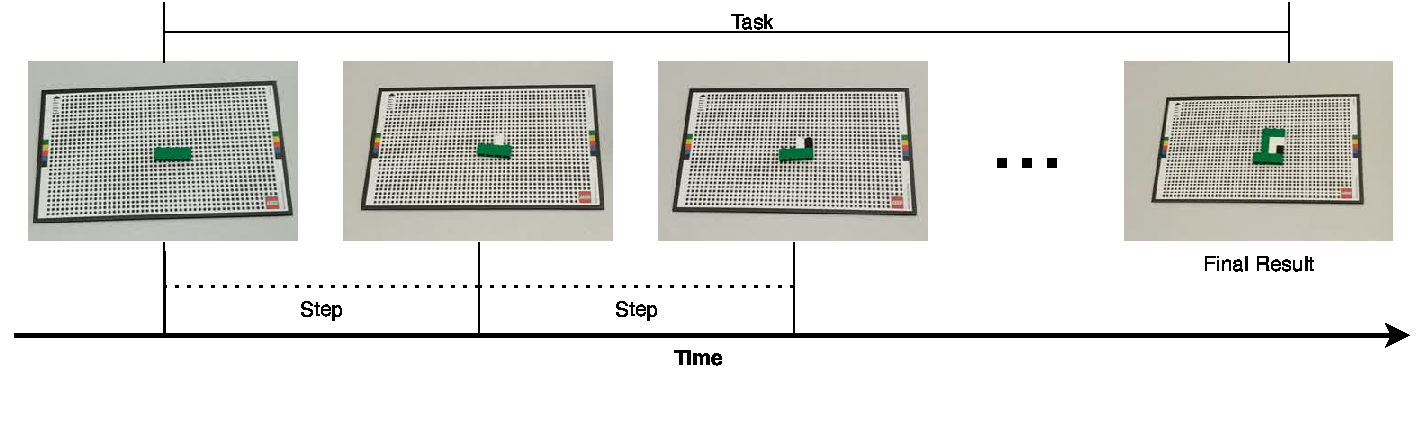
\includegraphics[width=.8\textwidth]{publications/2021ImpactDelayedResponse/Fig2.eps}
  \caption{Example of a Cognitive Assistance task and its component steps.}\label{paper:olguinmunoz2021impact:fig:task:steps}
\end{figure*}

% \begin{definition}[Step]

% While the subtask remains unfinished, the assistant discards results of the processing of the sampled inputs.
% At the beginning of a step, an instruction is given to the user.
% The user then proceeds to perform the subtask specified by the instruction, while the cognitive assistant is continuously sampling the subtask state at specified intervals. 

% Once the user finishes the required action, the next sample taken will contain a valid input, and thus the cognitive assistant will provide a new instruction. 
% This finishes the current step and potentially begins a new one if there remain instructions to be performed in the task.
% \end{definition}

In the base LEGO Assistant, the task consists of the assembly of a LEGO model; each step requires the user to append a LEGO brick to the model at a specific location and orientation.
The system monitors progress through a video feed and provides timely feedback in the form of visual and textual instructions to guide the user. 

The LEGO assistant has features that make it a good target for assessment of delay effects in a cognitive assistant.
In particular
\begin{inlineenum}[itemjoin={{, }},
                  itemjoin*={{, and }},
                  label={{(\arabic*)}}]
    \item it is easily understood by users and requires essentially no training
    \item its step-by-step nature simplifies the isolation of the relevant experimental variables and the effects of the delay
    % \item The states of the display can be recognized by simple image processing algorithms and do not require extensive training as for machine-learning-based applications.
    \item each step has an intrinsic hierarchical cognitive structure (see \cref{paper:olguinmunoz2021impact:fig:lego:hierarchical}), affording multiple levels of cognitive control.
\end{inlineenum}

\begin{figure*}[h]
  \centering
  % \begin{tikzpicture}[grow=down, scale=.6]
    \tikzset{edge from parent/.style= 
            {draw, thick, edge from parent fork down},
            every tree node/.style=
            {draw,very thick,align=center,scale=1,fill=black!10!white},
            every leaf node/.style=
            {fill=green!60!black!25!white,text width=2cm,minimum width=2cm},
            level distance=1in,sibling distance=.05in,
            execute at begin node=\strut
            }

    \node[draw,dashed,align=center](command){
        \footnotesize{Example instruction:}\\
        \small\textbf{``Find a $1 \times 1$ black piece and add it to}\\
        \textbf{the top right of the current model.''}
    % \\
    % \large{\textbf{``Remove the $1 \times 3$ red piece from the top of the current model.''}}
    };

    \begin{scope}[shift={($(command.south)+(0,-.25in)$)}]
        \Tree [.\node[fill=red!50!white]{\textbf{\Large{Change model}}};
                \node[diamond, aspect=2, fill=yellow!25!white](choice){Add or remove a piece?};
                ]
    \end{scope}

    \begin{scope}[shift={($(choice.west)-(1.5in,0)$)}]
        \Tree [.\node[draw=none, fill=none](add){Add a piece};
                [.{Select piece $X$} 
                    {Set $X$ size and color}
                    {Search box for matching pieces} ]
                [.{Select location $Y$} 
                    {Set $Y$ vertical and horizontal position}
                    {Find location on model} ]
                [.{Place $X$ at $Y$} 
                    {Pick up $X$ and move to model}
                    {Attach $X$ to model} ]
            ]
    \end{scope}

    \begin{scope}[shift={($(choice.east)+(1.5in,0)$)}]
        \Tree [.\node[draw=none, fill=none](remove){Remove a piece};
                \node[draw=none, fill=none]{\Huge{\ldots}}; 
                % [.{Select location $Y$} 
                %     {Set $Y$\\vertical and\\horizontal\\position}
                %     {Find\\location\\on model} ]
                % [.{Select piece $X$ at $Y$}
                %     {Set $X$\\size and\\color}
                %     {Search $Y$ for\\matching\\pieces} ]
                % [.{Remove piece $X$} 
                %     {Detach\\$X$}
                %     {Return $X$\\to box} ]
            ]
    \end{scope}

    \draw [thick] (choice.west) -- (add.east);
    \draw [thick] (choice.east) -- (remove.west);

\end{tikzpicture}%
  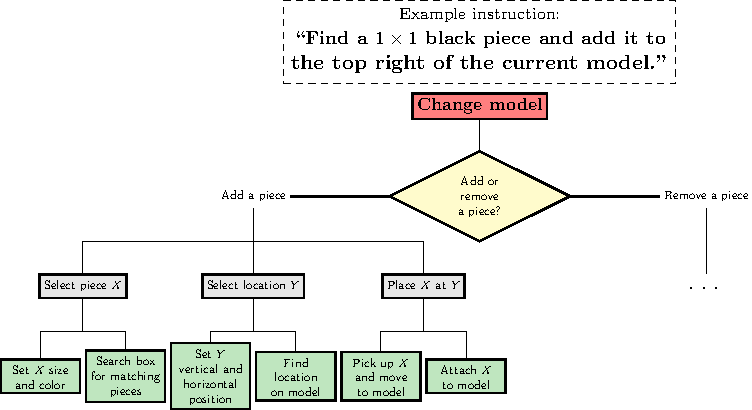
\includegraphics[width=\textwidth]{publications/2021ImpactDelayedResponse/Fig3.eps}
  \caption{Hierarchical cognitive structure of a step in the LEGO task.}
  \label{paper:olguinmunoz2021impact:fig:lego:hierarchical}
\end{figure*}


% The original design of the LEGO assistance application was based on a client-server model communicating over a wireless network, with the client software running on a wearable device and the server software deployed on a cloudlet. 
For the purposes of this study, the original client-server design of the LEGO Assistant was altered to be locally executable.
This was done in order to eliminate the stochastic effects of jitter and latency from the network link, and greatly simplify instrumentation.
% By this means, we achieve much more fine-grained control over the latencies to which the system is subject.
% Additionally, this greatly simplified the instrumentation of the application.
Instructions were output in image and text form to a computer display situated on a table directly in front of the participants.
Participants performed the instructions on the table, these actions being captured by a high-definition camera located on top of the display.

% Finally, a data collection and experimental layer was implemented between the user interface and video capture and the core processing component of the LEGO Assistant.
% This layer controlled the manipulated experimental variables and recorded the measured biometric and task-related effects.

\subsection{The Experimental LEGO Task}

For the experimental LEGO task, a key modification was made to the structure of the steps.
After each the processing of each input is completed, the result is withheld for a variable period of time until a specific target \emph{delay} is reached, as illustrated in \cref{paper:olguinmunoz2021impact:fig:cogassist:step,paper:olguinmunoz2021impact:fig:cogassist:step:delay}.
The length of this delay is one of two independent variables we manipulated for the experiment.
Seven levels of delay were used --- no added delay (which we will also refer to as \SI{0}{\second} delay), \SIlist{0.6;1.125;1.65;2.175;2.7;3.0}{\second} --- chosen based on the latency bounds found previously by Chen et al.~\cite{chen2017empirical}.
% A value of  \SI{600}{\milli\second} was identified as the bound where users start noticing delays in the assistant.
% Conversely, \SI{2.7}{\second} was identified as the upper bound on delays after which the application is considered to be in such a degraded state it is basically ``unusable''.
Our selection of delays is centered around the range of delays where latency is noticeable to users, but the application remains in a ``usable'' state.
% while including one delay value in the unnoticeable range and one completely in the ``unusable'' range.

In order to study the effects of a delay applied across multiple steps we implement an experimental design component called a \emph{block}, corresponding to a sequence of consecutive steps within a task subject to the same delay; see \cref{paper:olguinmunoz2021impact:fig:cogassist:block}.
% \begin{definition}[Block]
%   A sequence of consecutive steps within a task subject to the same delay; see \cref{paper:olguinmunoz2021impact:fig:cogassist:block}.
The \emph{length} of blocks is the second of the two independent variables manipulated in our experiment.
We used values of \numlist{4;8;12} steps, chosen as representative of the number of steps in tasks in the base LEGO Assistant application.
Additionally, we define the \emph{duration} of a block, as the time elapsed between the start timestamp of the first step in the block and the end timestamp of the final step in the block.
% ; e.g.\ for \cref{fig:cogassist:block}, the duration of the pictured block would be \( t_{n+k} - t_{n} \).
% \end{definition}

To assign tasks to the participants, a pseudo-random permutation of the combinations of block length and delay was first generated, and a unique sequence of steps assigned to each of these combinations to create 21 unique blocks.
A \emph{Latin~square}-type design was then used to reorder this initial permutation in order to generate a task for each participant.
This ensures a counterbalance of the order of the blocks across participants and avoids systematic learning effects. 
% The design rotates the block types (as defined by length and delay) across participants so that each type is tested in each ordinal position, but it only coarsely samples from the \( 21 \times 20 \) possible sequences from one block type to another.
Note that unlike the base LEGO assistant task, in which instructions led participants through the assembly of a specific model, the experimental LEGO task consisted of a sequence of instructions to either add or remove pieces with no evident goal.
% Users were directed to either add a piece to the ongoing model or to remove a piece, and blocks were designed in such as way so as to ensure that the transitions between them were invisible to the user. 

% In this paper we will thus consider blocks to be our basic element of study, and most aggregations will be done at this level (with a few exceptions).
% For this, we will need additional definitions:

% \begin{definition}[Delay associated with a block]
%   We will refer to the delay of a block as the delay applied to every frame of every step in that block.
% \end{definition}

% \begin{definition}[Execution time]

Given the variability in the system latency to detect step completion, correcting step-completion time for system response time by a fixed amount would not enable sufficient precision.
We therefore define the \emph{execution time} empirically for an individual step as the total time between the user receiving the instruction for the step and the time instant of the sample capturing the completed step.
% their presenting the completed subtask to the system.

% We define the \emph{execution time} of a step as the time between the user receiving an instruction for a subtask and them presenting the completed subtask to the system.
% This, however, could not be measured directly and has to be inferred from the records of inputs processed by the system.

For an arbitrary step, we define the sequence \( \{ t_{0}, t_{1}, \ldots, t_{n} \} \) as the sequence of timestamps corresponding to the sampling instants during the step (see \cref{paper:olguinmunoz2021impact:fig:exectime:diagram}).
\( t_{0} \) corresponds to the instant when the instruction for the step is given to the user (and the first sample is taken), and \( t_{n} \) to the timestamp of the last sample before a new instruction is given.
If we define \( t_{c} \) as the instant marking when the user presented the finished step to the system, it must follow that \( t_{n-1} < t_{c} < t_{n} \).
Due to the discrete sampling of the task state, there remains some imprecision in the estimate of execution time relative to \( t_{c} \).
However, this introduces no bias in the results, as we can assume that \( t_{c} \) is uniformly distributed in the range \( (t_{n-1}, t_{n}) \).
We therefore calculate execution time for each step as \( t_{c} - t_{0},\; t_{c} \in U(t_{n-1}, t_{n}) \), which on average works out to an adjustment of the observed time by 1.5 times the mean sampling rate of the step.
% This is also aggregated into an average at the block level.

% \begin{figure}
%   \centering
%   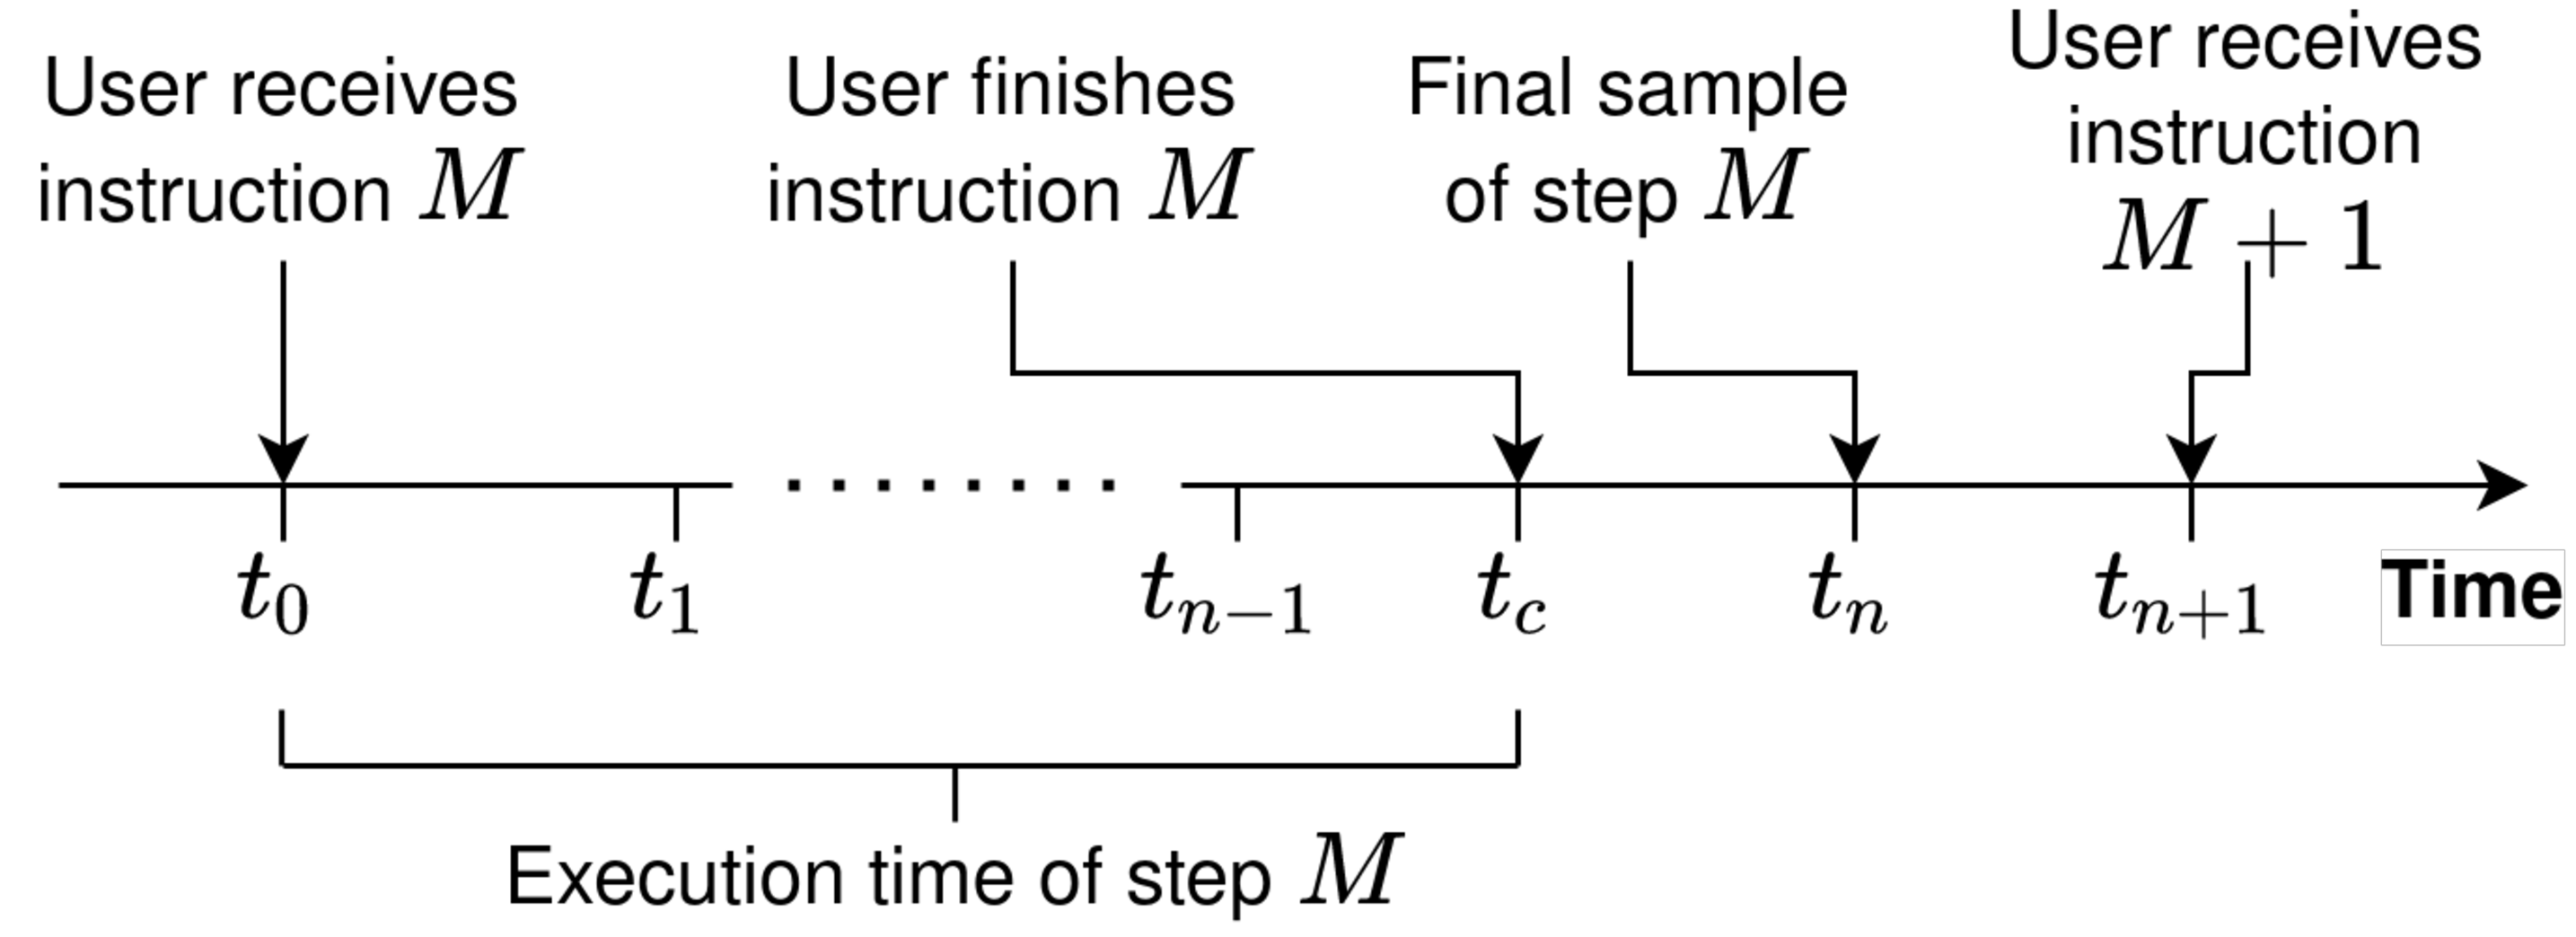
\includegraphics[width=.85\textwidth]{images/exec_time_diagram.pdf}
%   \caption{Visualization of the execution time of a step.}%
%   \label{paper:olguinmunoz2021impact:fig:exectime:diagram}
% \end{figure}

% \end{definition}

\begin{figure}[h]
  \centering
  \begin{subfigure}[t]{.49\textwidth}
    \centering
    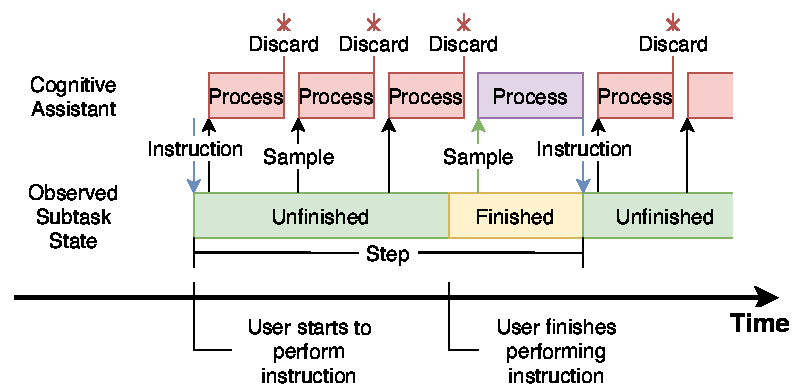
\includegraphics[width=\textwidth]{publications/2021ImpactDelayedResponse/Fig4a.eps}
    \caption{Structure of a step in a generic cognitive assistance application. 
    The assistant provides an instruction to the user and continuously samples the step state; inputs captured while the step is unfinished are silently ``discarded'' (i.e.\ they do not cause the generation of a new instruction).
    % by the assistant, as they do not contain relevant information.
    Once the user finishes performing the step, the next sample \emph{will} cause the generation of a new instruction.
    % which will subsequently be provided to the user.}%
    }
    \label{paper:olguinmunoz2021impact:fig:cogassist:step}
  \end{subfigure}%
  % \medskip%
  \hfill%
  \begin{subfigure}[t]{.49\textwidth}
    \centering
    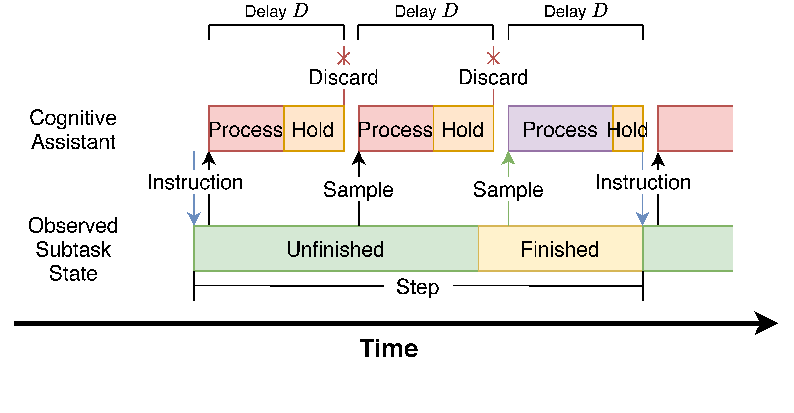
\includegraphics[width=\textwidth]{publications/2021ImpactDelayedResponse/Fig4b.eps}
    \caption{In the experimental task, an additional variable segment of time is introduced immediately following the processing of the input frame in order to extend the perceived processing time of the input to a specific target delay.}%
    \label{paper:olguinmunoz2021impact:fig:cogassist:step:delay}
  \end{subfigure}
  \medskip%
  \begin{subfigure}[t]{.49\textwidth}
    \centering
    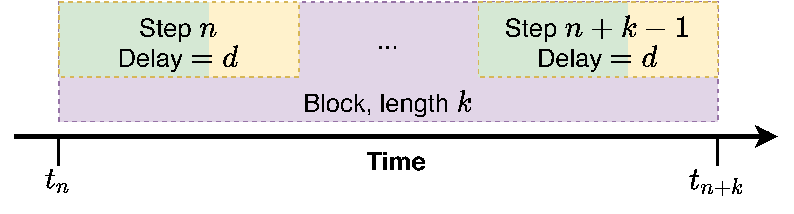
\includegraphics[width=\textwidth]{publications/2021ImpactDelayedResponse/Fig4c.eps}
    \caption{Structure of a block in the experimental task.}%
    \label{paper:olguinmunoz2021impact:fig:cogassist:block}
  \end{subfigure}%
  % \medskip%
  \hfill%
  \begin{subfigure}[t]{.49\textwidth}
    \centering
    \includegraphics[width=\textwidth]{publications/2021ImpactDelayedResponse/Fig4d.eps}
    \caption{Visualization of the execution time of a step.}%
    \label{paper:olguinmunoz2021impact:fig:exectime:diagram}
  \end{subfigure}%
  % \medskip%
  \caption{Components of the cognitive assistance task.}
\end{figure}

\subsection{Collected Data}

The collected data from the experiments fall into four categories: behavioral and personality indicators, \emph{frame-to-frame} metrics, biometric data, and video recordings.

\subsubsection{Behavioral and Personality Indicators}

Before beginning the experimental procedure, participants were asked to fill out two questionnaires.

The first of these, the \gls{BFI}~\cite{john1999big}), consists of 44 questions to be answered on a 5-point \emph{Likert}-type scale, assessing the traits of \emph{agreeableness: detached to compassionate} (8 questions), \emph{conscientiousness: careless to organized} (9 questions), \emph{extroversion: reserved to outgoing} (8 questions), \emph{neuroticism: secure to sensitive} (8 questions), and \emph{openness: cautious to curious} (9 questions).
Of these, extroversion and neuroticism have been related to tolerance for delay~\cite{hirsh2008delay}. 

The second survey, the \gls{ITQ}~\cite{witmer1998measuring}), comprises 29 questions, 28 of which were used for the study (one categorical question was disregarded), assessing the sub-scales of \emph{involvement}, the tendency to become involved in activities; \emph{focus}, the tendency to maintain focus on current activities, and \emph{games}, the tendency to play games.
These questions use a 7-point horizontal scale  with opposing descriptors anchoring  the ends.
Participants were asked to mark the appropriate point in the scale, and these responses were converted to a numerical value between 1 and 7 for processing. 

In post-processing, the obtained scores for both questionnaires were normalized to fall in the \( [0, 1] \) range for ease of interpretation. 
See \cref{paper:olguinmunoz2021impact:tab:qscores} for their means and standard deviations.

\begin{table}[h]
  \centering
  \caption{Means and standard deviations of normalized questionnaire scores.}\label{paper:olguinmunoz2021impact:tab:qscores}
  \setlength{\tabcolsep}{0pt} 
  \begin{tabular*}{\columnwidth}{@{\extracolsep{\fill}\quad}clrr@{}}
    \toprule
    \textbf{Questionnaire} & \textbf{Metric} & \textbf{Mean} & \textbf{SD}\\
    \midrule
    \multirow{5}{*}{\gls{BFI}}
        & Agreeableness &               0.705 &                  0.136 \\
        & Conscientiousness &               0.562 &                  0.149 \\
        & Extroversion &               0.491 &                  0.180 \\
        & Neuroticism &               0.524 &                  0.230 \\
        & Openness &               0.677 &                  0.152 \\
    \cline{1-4}
    \multirow{4}{*}{\gls{ITQ}}
        & Focus &               0.626 &                  0.126 \\
        & Games &               0.463 &                  0.261 \\
        & Involvement &               0.568 &                  0.175 \\
        & Total &               0.540 &                  0.092 \\
    \bottomrule
  \end{tabular*}
\end{table}


\subsubsection{Frame-to-frame metrics}
During the execution of the task, we logged every event occurring in the application pipeline.
Each incoming frame (including frames discarded by the assistant), as well as its associated outputs, was logged at multiple points in the process along with associated metadata such as currently implemented delay as specified by the experimental design.
This allowed us to extract metrics relating to the performance of the task, such as the time spent by participants on particular steps, any mistakes made, etc.
In particular, it made possible the easy segmentation of the other time-series data we collected into our main unit of analysis, the aforementioned \emph{block}.

\subsubsection{Biometric Data}
The participants wore devices to acquire four physiological measures:
\begin{inlineenum}[itemjoin={{, }},
                  itemjoin*={{, and }},
                  label={{(\arabic*)}}]
  \item \glsreset{GSR}\gls{GSR}
  \item accelerometer data from the dominant wrist
  \item brain activity in the form of \glsreset{EEG}\gls{EEG}
  \item heart rate.
\end{inlineenum}

These metrics have been used as indicators of stress and cognitive load by an ample body of previous research~\cite{khawaji2015using,kuikkaniemi2010influence,solovey2014classifying}.
\gls{GSR} (also known as electrodermal activity) can be interpreted as an indicator of physiological arousal and has long been a widely used metric in studies seeking to characterize mental workload~\cite{peterson1907psycho,healey2005detecting,son2010age,khawaji2015using,kuikkaniemi2010influence,solovey2014classifying}.
\gls{EEG} on the other hand has previously been used to measure cognitive load in the context of human-computer interactions~\cite{antonenko2010using,grimes2008feasibility,kumar2016measurement}.

Wrist acceleration, \gls{GSR} and heart rate data were obtained using the Empatica E4~\cite{empatica:e4} biosensing wristband.
Accelerometer data was sampled at \SI{32}{\hertz},
\gls{GSR} was sampled at \SI{4}{\hertz}, and instantaneous heart rate was calculated from a \emph{blood volume pulse} signal sampled at \SI{64}{\hertz}.
Participants were asked to wear the device for approximately 10--15 minutes before starting the experiment, in order to allow the sensors to reach a stable equilibrium and establish a baseline for the signals.

The E4 wristband was chosen due to its small, non-invasive, and wireless form factor (samples were streamed to the system over Bluetooth LE) and for the fact that its use in research has been experimentally validated in previous studies~\cite{ragot2017emotion, mccarthy2016validation}.
The E4 also includes a skin temperature thermometer, however the measure was not used for the present study.

For the \gls{EEG} data we employed the OpenBCI \gls{EEG} Headband Kit~\cite{openbci:headbandkit} consisting of a number of dry electrodes fastened to a Velcro headband.
It provides a quick and non-invasive way of obtaining \gls{EEG} signals from participants.
Electrodes were placed according to the \emph{10--20 Electrode System}~\cite{eeg1020system:1961} on the \emph{Fp1} and \emph{Fp2} points, in order to capture brain activity in the frontal lobe, with ground and reference electrodes on the right and left earlobes, respectively.
The signals were sampled at \SI{200}{\hertz} and postprocessed to 
\begin{inlineenum}[itemjoin={{, }},
                  itemjoin*={{, and }},
                  label={{(\arabic*)}}]
  \item remove frequencies outside the \SIrange{0.1}{40}{\hertz} range
  \item smooth out noise (using the technique proposed by Agarwal et al.~\cite{agarwal2017eeg}).
\end{inlineenum}

\subsubsection{Video recordings}

During the task, participants were recorded by two separate cameras.
One camera was angled downwards, towards the table, the LEGO board, and the participant's hands.
This camera was used to capture the necessary inputs for the LEGO assembly task as well as to record the actions performed by the user.
The second camera was angled horizontally, towards the participant, in order to record their facial expressions during the execution of the task.

Both video feeds were captured at a rate of \num{24}~\gls{FPS} in parallel processes to ensure a constant rate of capture.
Examples of the captured frames can be seen in \cref{paper:olguinmunoz2021impact:fig:sampleframes}.
The video feeds were not used for the present study, but may be utilized in future analysis.

\begin{figure}[h]
  \centering
  \begin{subfigure}[t]{.35\textwidth}
    \centering
    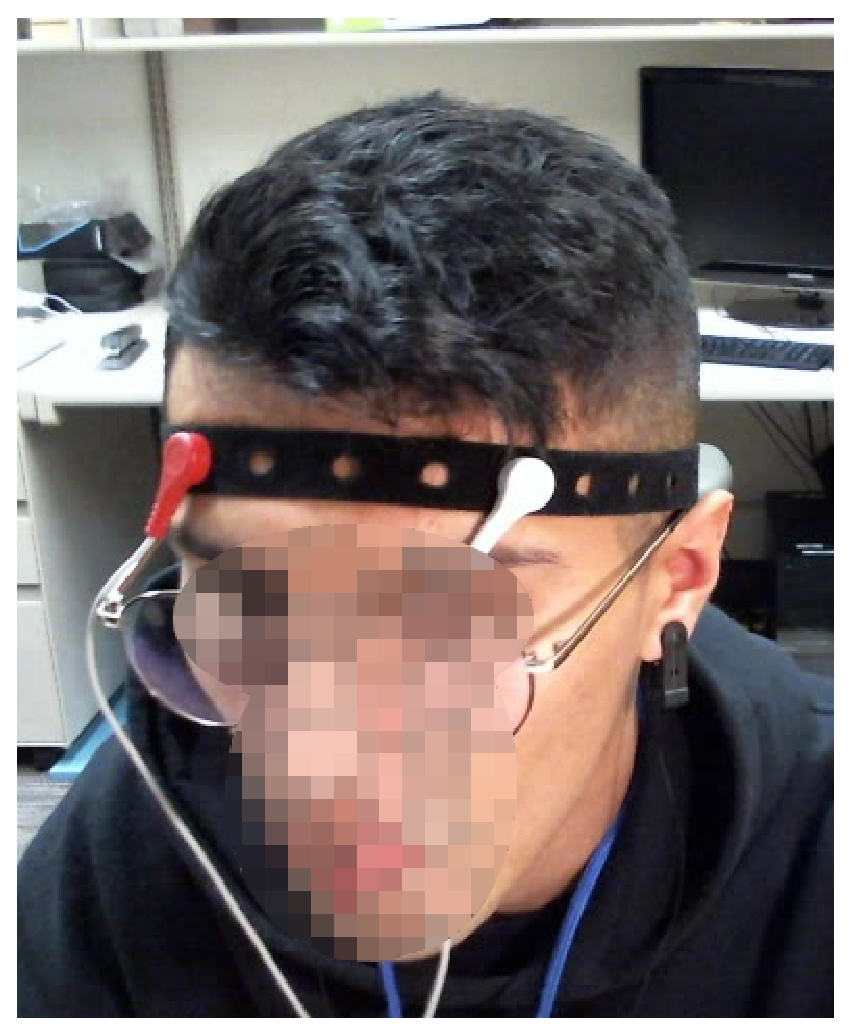
\includegraphics[height=140pt]{publications/2021ImpactDelayedResponse/Fig5a.eps}
    \caption{Frame from the face recording of a random participant, clearly showing the locations of the \gls{EEG} electrodes.}
  \end{subfigure}%
  % \par\bigskip
  % \hspace{.04\textwidth}%
  \hfill%
  \begin{subfigure}[t]{.60\textwidth}
    \centering
    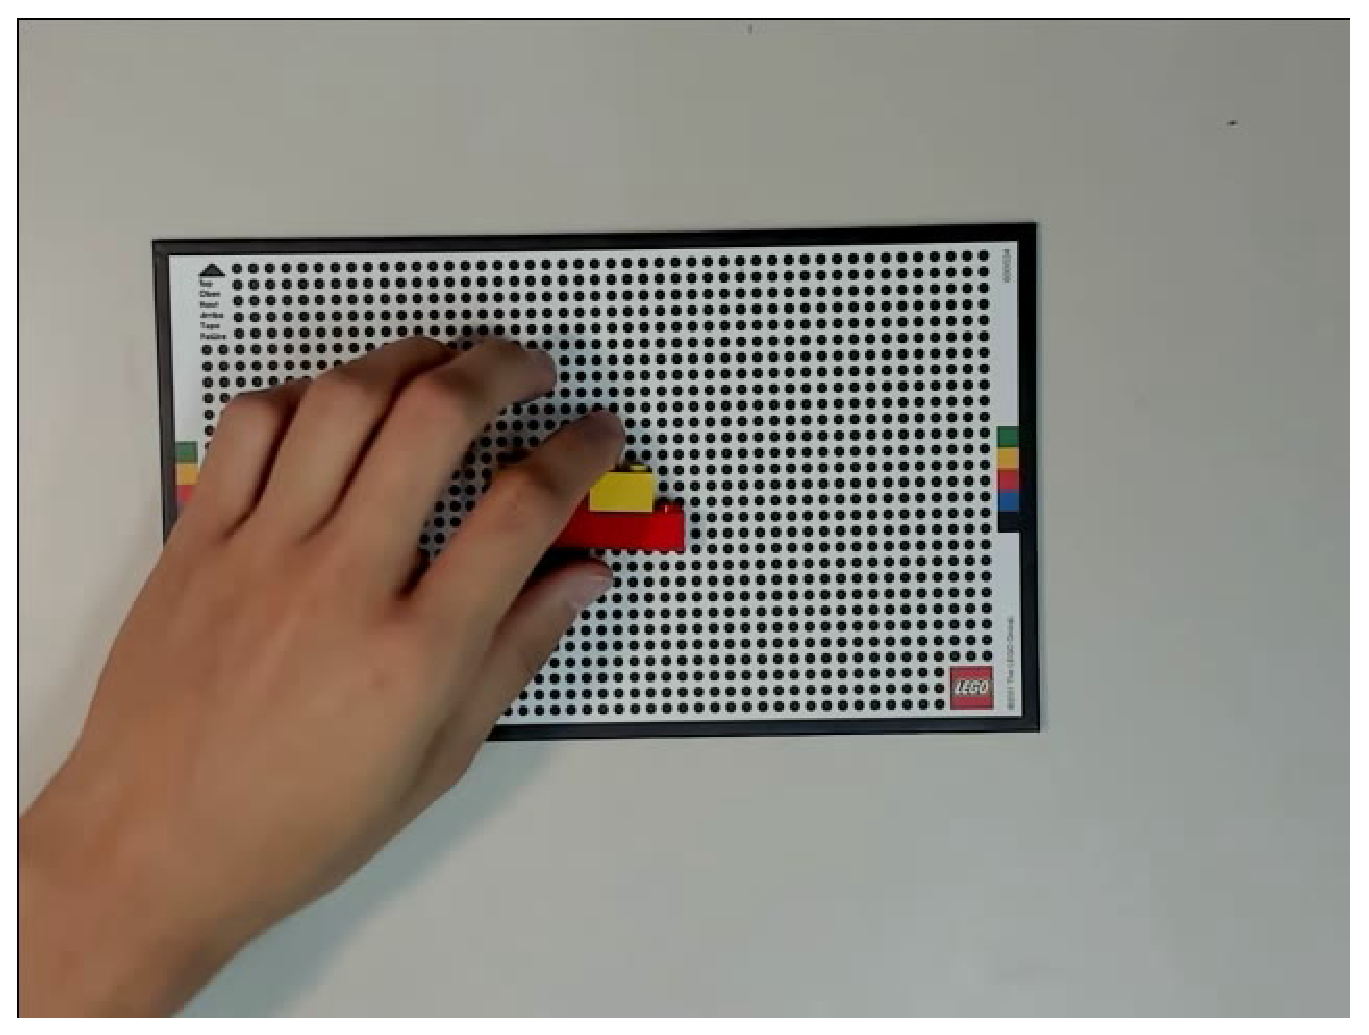
\includegraphics[height=140pt]{publications/2021ImpactDelayedResponse/Fig5b.eps}
    \caption{Frame from the board recording of the same participant.}
  \end{subfigure}
  \caption{Sample frames captured during the experiment.}\label{paper:olguinmunoz2021impact:fig:sampleframes}
\end{figure}

\section{Results}\label{paper:olguinmunoz2021impact:sec:results}

The results consist of execution time per step. and the outcome of physiological variables: heart rate, \gls{GSR}, and \gls{EEG}.\@
Each will be discussed in turn.
%The temperature data could not be analyzed due to a progressive increase in the sensor data over the course of the session, which obscured effects of the experimental variables.

\subsection{Execution Time}

% Before describing the analysis and results relating to execution time, it should be noted that accuracy for this metric was essentially perfect.
% No mistakes were made by participants during the execution of the task and no major outliers could be identified in the samples.

Before describing the analysis and results relating to execution time, it should be noted that participants' performance during the execution of the task was error free; all steps were completed as instructed. 

\cref{fig:exectime} shows the mean per-step execution time per block, averaged over block length (number of steps) and artificial delay.
We can clearly see a trend for the execution time to increase with the delay, increasingly so for longer blocks. 
Since the per-step execution time  compensates for the added delay in the measure \emph{per se}, this trend must result from the participants' behavioral adjustment to the delay.
This leads to one of the key outcomes from this study: 
\emph{participants tend to act more slowly on steps affected by longer delays} --- i.e.\ there is evidence of a pacing effect in users' behavior with respect to the responsiveness of the system.

We confirmed this effect through an \gls{ANOVA}~\cite{fujikoshi1993two} with factors of block length and delay, and found significant main effects of both factors and the interaction, shown in \cref{paper:olguinmunoz2021impact:tab:anova:exectime}.
% An ANOVA test uses the \emph{F-test} statistic, which is a ratio of the variability in the data introduced by experimental manipulations (and their interactions) to the variability in the data attributable to randomness.
% The degrees of freedom represent the number of observations going into each of these variability measures.
% As we are using within-subject designs, the variability in the data due to randomness is estimated by the differences among subjects with respect to the effects of the experimental variables.
% The partial-\( \eta^2 \) (\(\eta_{p}^{2}\)) statistic is a measure of effect size, corresponding to the proportion of variance explained by the effect after excluding variance from others, and \( p \)-value, a measure of the probability of the effect under the null hypothesis.
% Conventionally \( p < .05 \) is the criterion for significance.
% The current length \( \times \) delay ANOVA found significant main effects of both factors and the interaction, shown in \cref{paper:olguinmunoz2021impact:tab:anova:exectime}.

% \begin{figure}[h]
%     \centering
%     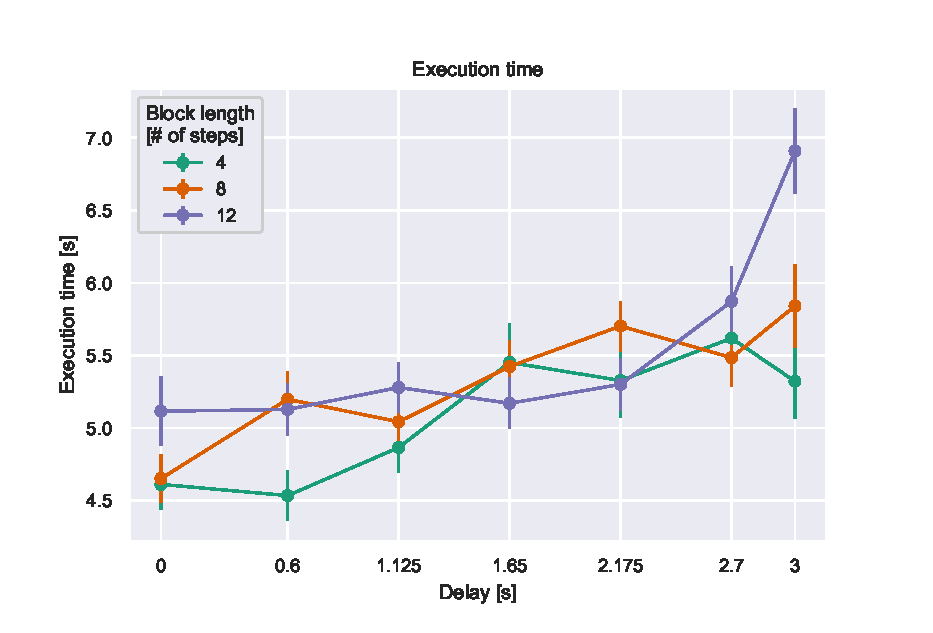
\includegraphics[width=.8\textwidth]{plots/exec_time_delay_length.eps}
%     \caption{Per-step execution time by block length vs.\ delay. Error bars indicate the Standard Error of the Mean (S.E.M.)}\label{fig:exectime}%    
% \end{figure}

\begin{figure}[h]
    \centering
    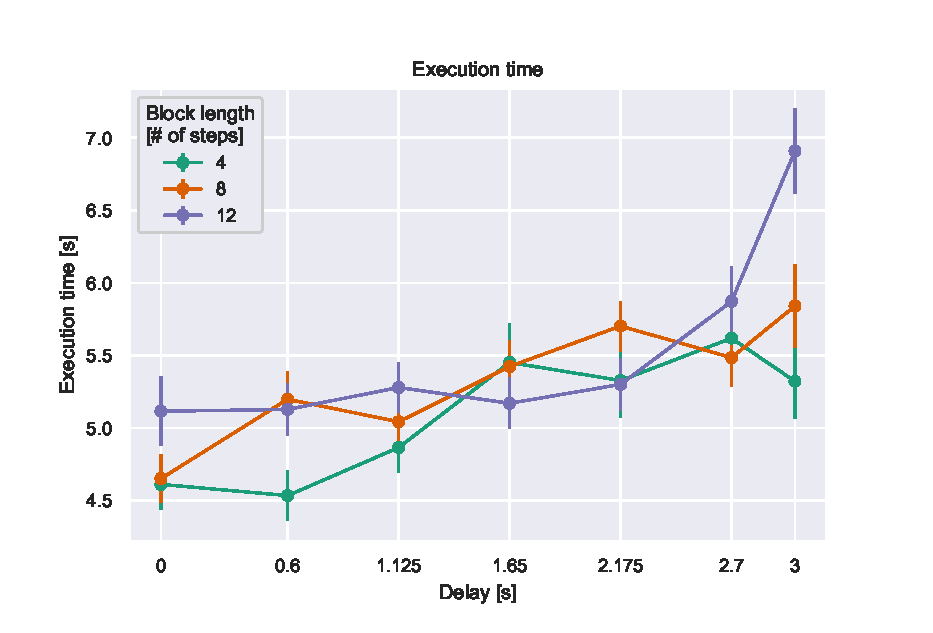
\includegraphics[width=.8\textwidth]{publications/2021ImpactDelayedResponse/Fig6.eps}
    \caption{Per-step execution time by block length vs.\ delay. Error bars indicate the \gls{SEM}}\label{fig:exectime}%
\end{figure}

\begin{table}[h]
  \centering
  \caption{Significant effects on per-step execution time from \gls{ANOVA} on factors delay and block length.}\label{paper:olguinmunoz2021impact:tab:anova:exectime}
  \setlength{\tabcolsep}{0pt}%
  \begin{tabular*}{\columnwidth}{@{\extracolsep{\fill}\quad}lrrr@{}}
    \toprule
    \textbf{Factor} & \textbf{F-test} & \( p \) & \( \eta^{2}_{p} \) \\
    \midrule
    length         &    \(F(2, 78) = 9.59\) &   \(< 0.001\) &           \(0.20\) \\
    delay          &  \(F(6, 234) = 15.52\) &  \(< 0.0001\) &           \(0.28\) \\
    length \(\times\) delay &  \(F(12, 468) = 3.84\) &  \(< 0.0001\) &           \(0.09\) \\
    \bottomrule
  \end{tabular*}
\end{table}

Further analysis focused on the progressive effect on per-step execution time as additional steps occurred at a constant delay.
For this purpose, the steps within a block were aggregated over sequences of 4, constituting a \emph{slice}.
Note that the first slice within a block is procedurally identical for all block lengths, in the sense that a participant currently performing a step in the first slice of a block has no way of predicting if the block ends after step 4 or not.
The same logic can be applied to slice 2 for blocks of length 8 and 12.
Accordingly for each participant, slice 1 data (steps 1--4) were pooled over all 3 block lengths, slice 2 (steps 5--8) were combined for block lengths 8 and 12, and slice 3 comprised the last four steps in blocks of length 12.
An \gls{ANOVA} on slice number (1--3) and delay (7 values) yielded effects of slice number, delay, and the interaction, detailed in \cref{paper:olguinmunoz2021impact:tab:anova:exectime:slice}.
As shown in \cref{paper:olguinmunoz2021impact:fig:exectime:delay:slice}, blocks with shorter delays showed a trend for the execution time to progressively decline over the course of the block (i.e., by slice number), indicating that the participant accommodated to the feedback pace with more efficiently timed responses.
% We refer to the measure at slice 3 as a percentage of the measure at slice 1 as the ``change factor''.
With the longest delays, where the execution time per step was longest, the slow-down persisted; that is, the system response time hindered the participant's execution throughout the course of the block.

\begin{table}[h]
  \centering
  \caption{Significant effects on per-step execution time from \gls{ANOVA} on factors block slice and delay.}\label{paper:olguinmunoz2021impact:tab:anova:exectime:slice}
  \setlength{\tabcolsep}{0pt} % let TeX compute the intercolumn space
  \begin{tabular*}{\columnwidth}{@{\extracolsep{\fill}\quad}lrrr@{}}
    \toprule
    \textbf{Factor} & \textbf{F-test} & \( p \) & \( \eta^{2}_{p} \) \\
    \midrule
    slice         &   \( F(2, 78) = 88.79 \) &  \( < 0.0001 \) &         \( 0.69 \) \\
    delay         &  \( F(6, 234) = 14.13 \) &  \( < 0.0001 \) &         \( 0.27 \) \\
    slice \( \times \) delay &  \( F(12, 468) = 2.49 \) &    \( < 0.01 \) &         \( 0.06 \) \\
    \bottomrule
  \end{tabular*}%
\end{table}

\begin{figure}[h]
    \centering
    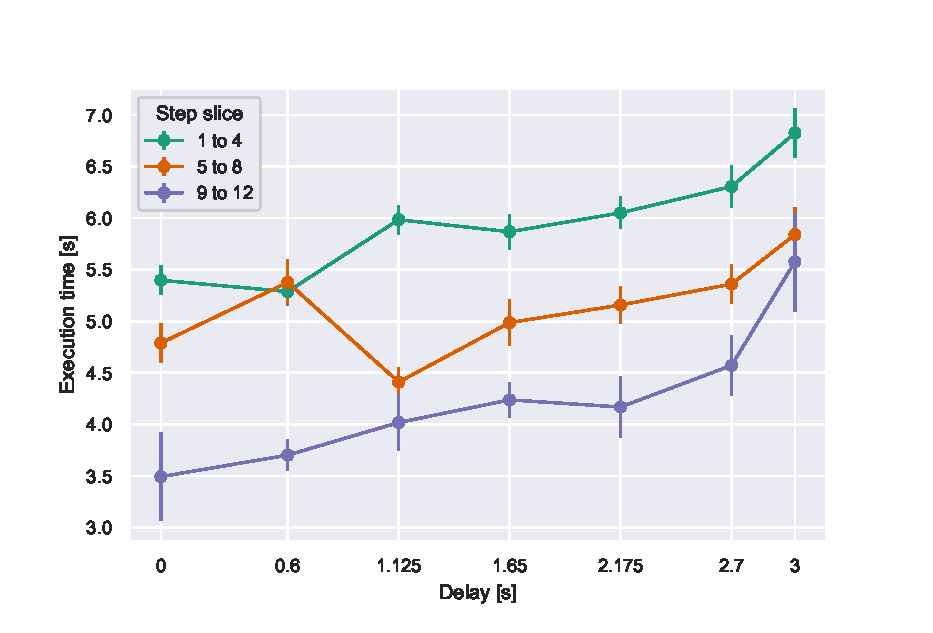
\includegraphics[width=.8\textwidth]{publications/2021ImpactDelayedResponse/Fig7.eps}
    \caption{Mean per-step execution time vs.\ delay, by step slice.
    Error bars indicate \gls{SEM}}
    \label{paper:olguinmunoz2021impact:fig:exectime:delay:slice}
\end{figure}

The data also allowed us to perform sub-analyses to assess the effects of carryover from one delay to another.
Specifically, we measured the per-step execution time for the first four steps of a block when participants transferred from a relatively long delay (\SIrange{2.175}{3.0}{\second}) versus a short delay (\SIrange{0}{1.65}{\second}).
Note that use of the first four steps controls for block length.
We performed analyses where participants transitioned from either a short- or long-delay block into a
\begin{inlineenum}[label=(\roman*), before=\unskip{: }, itemjoin={{; }}, itemjoin*={{; and }}]
  \item no delay block (36 subjects)
  \item \SI{1.65}{\second} delay block (40 subjects)
  \item \SI{2.7}{\second} delay block (40 subjects)
  \item \SI{3.0}{\second} delay block (37 subjects).
\end{inlineenum}
The destination delays were chosen so as to maximize the number of participants which contributed samples to the analyses, the results of which are pictured in \cref{paper:olguinmunoz2021impact:fig:exectime:transition}.
We found that transitions from long-delay blocks carried over to significantly increase the per-step execution time of initial steps in the destination block for three of the four transitioned-into delays that were assessed (\SIlist{0;2.7;3.0}{\second}, all \( p < .025\)).

\begin{figure}[h]
  \centering
  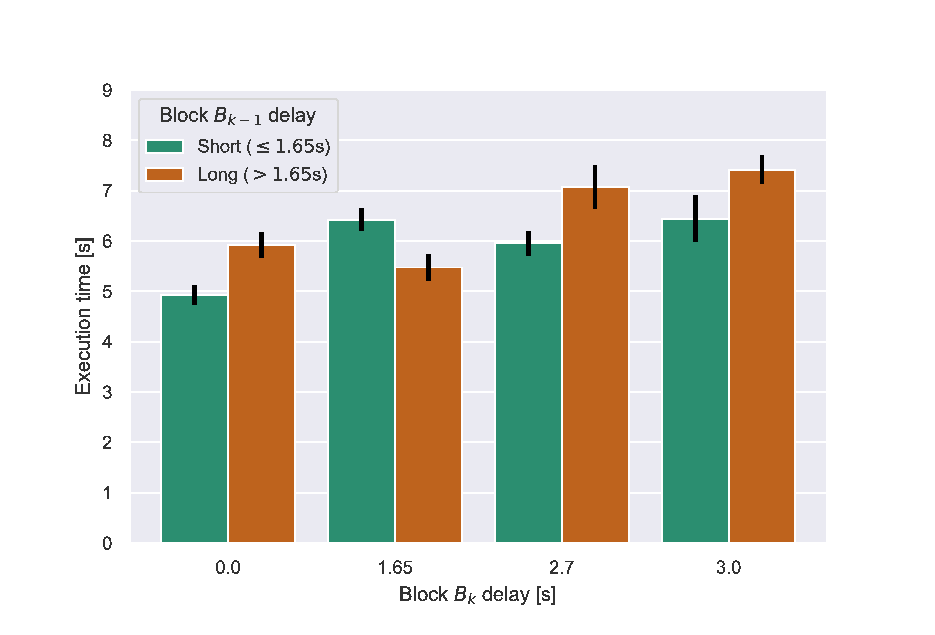
\includegraphics[width=.8\textwidth]{publications/2021ImpactDelayedResponse/Fig8.eps}
  \caption{Per-step execution time across the first four steps after a block transition from block \( B_{k-1} \) to \( B_k \). Error bars indicate \gls{SEM}}\label{paper:olguinmunoz2021impact:fig:exectime:transition}%
\end{figure}

In summary, we observe two direct effects on execution time due to added delays.
Firstly, we see a clear hampering of the improvement of execution time across steps that is otherwise evident across blocks.
Secondly, we notice that this effect lingers on even after the delay is removed, affecting subsequent blocks in the task.

\subsection{Acceleration}

Acceleration data from the E4 wristband were taken in 3 axes defined relative to the device.
As our interest was in the amount of movement rather than the direction in space, we calculated a ``movement score'' for each block which we defined as:
\begin{equation}
    M_B = \frac{ \sum_{A_B} |\: \overrightarrow{\alpha_j} \:| }{\Delta T_{B}}
\end{equation}

where \( B \) is an arbitrary block, and \(A_{B} = \{ \overrightarrow{\alpha_0}, \overrightarrow{\alpha_1}, \ldots, \overrightarrow{\alpha_k} \} \) represents the set of acceleration vector samples collected for said block.
This score would include the time imposed by the delay and the time to decode the instructions and respond by moving the pieces so that the next state was recognized.
It is only during the last part of the step that explicit movement is required, so any additional accelerations would derive from arbitrary movements while processing and waiting.
We normalized the sum of the accelerations by the duration of the step to correct for differences in delay and the execution time, which tends to increase with delay as described above.
An \gls{ANOVA} on block length and delay showed a significant effect such that movement score decreased with delay, as shown in \cref{paper:olguinmunoz2021impact:tab:anova:acc} and \cref{paper:olguinmunoz2021impact:fig:acc:delaylength}.
There was also a significant delay by length interaction, reflecting that delay effects occurred particularly for the longer lengths.

\begin{table}[h]
  \centering
  \caption{Significant effects on accelerometer data from \gls{ANOVA} on factors delay and block length.}\label{paper:olguinmunoz2021impact:tab:anova:acc}
  \setlength{\tabcolsep}{0pt} % let TeX compute the intercolumn space
  \begin{tabular*}{\columnwidth}{@{\extracolsep{\fill}\quad}lrrr@{}}
    \toprule
    \textbf{Factor} & \textbf{F-test} & \textbf{\(p\)} & \textbf{\(\eta^{2}_{p}\)} \\ 
    \midrule
    delay & \(F(6, 234) = 18.56\) & \(<0.001\) & \(0.32\) \\
    length \( \times \) delay & \(F(12, 468) = 3.04\) & \(<0.001\) & \(0.07\) \\ 
    \bottomrule
  \end{tabular*}%
\end{table}

\begin{figure}[h]
    \centering
    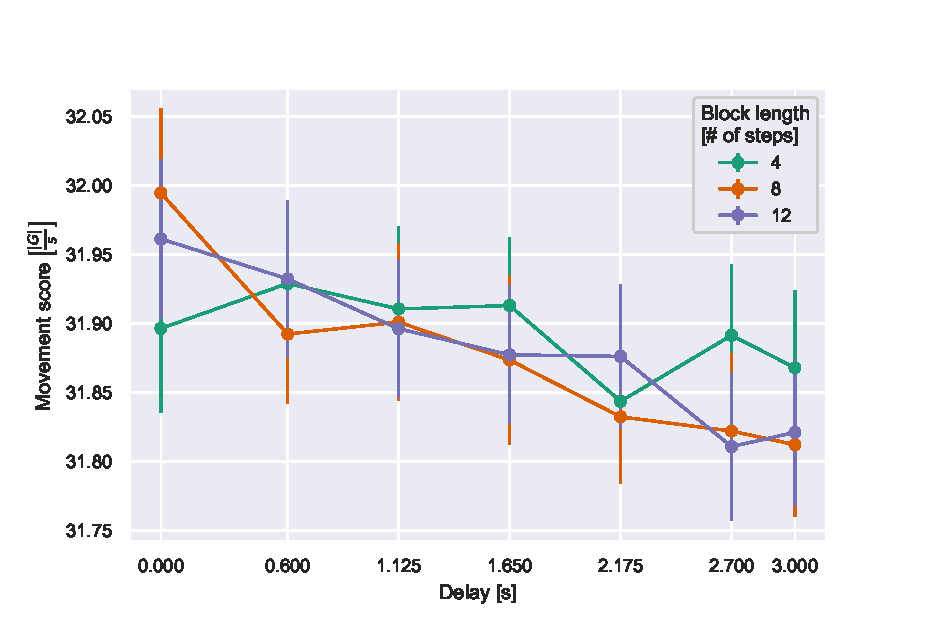
\includegraphics[width=.8\textwidth]{publications/2021ImpactDelayedResponse/Fig9.eps}
    \caption{Movement score vs.\ delay, per block length. Error bars indicate \gls{SEM}}\label{paper:olguinmunoz2021impact:fig:acc:delaylength}
\end{figure}

We next conducted the same analysis as for execution time, dividing blocks into three ``slices'' of four steps each, such that slice 1 comprised the first four steps of all block lengths, slice 2 the second four steps of blocks of length 8 and 12, and slice 3 the last four steps of blocks 12 steps long.
As shown in \cref{paper:olguinmunoz2021impact:fig:acc:delayslice} the effect of delay was attributable only to the later slices, yielding main effect of slice number and delay and an interaction (\cref{paper:olguinmunoz2021impact:tab:anova:acc:slice}).

\begin{figure}[h]
  \centering
  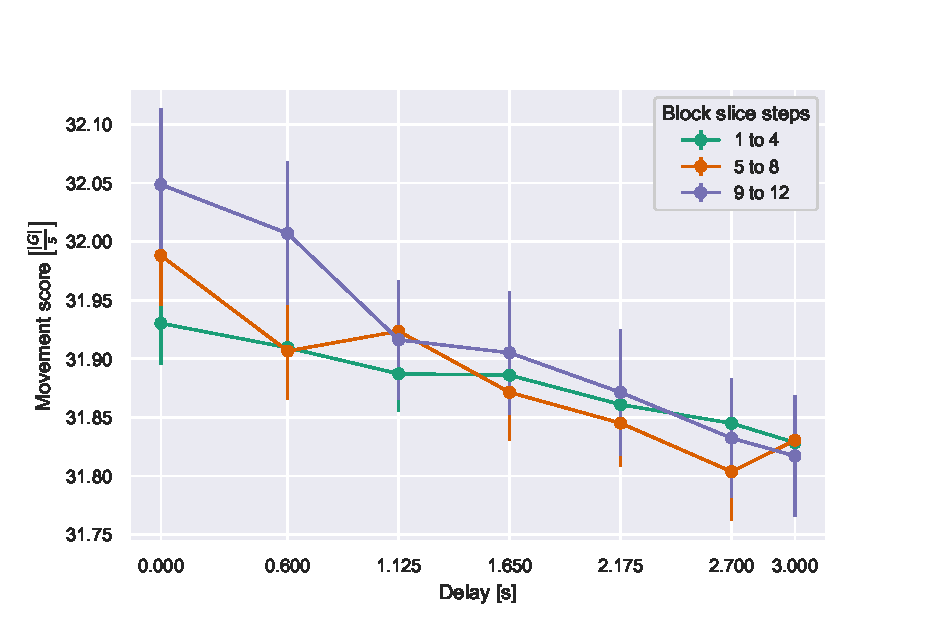
\includegraphics[width=.8\textwidth]{publications/2021ImpactDelayedResponse/Fig10.eps}
  \caption{Movement score vs.\ delay, per block slice. Error bars indicate \gls{SEM}}\label{paper:olguinmunoz2021impact:fig:acc:delayslice}
\end{figure}

\begin{table}[h]
  \centering
  \caption{Significant effects on accelerometer data from \gls{ANOVA} on factors delay and slice number.}\label{paper:olguinmunoz2021impact:tab:anova:acc:slice}
  \setlength{\tabcolsep}{0pt} % let TeX compute the intercolumn space
  \begin{tabular*}{\columnwidth}{@{\extracolsep{\fill}\quad}lrrr@{}}
    \toprule
    \textbf{Factor} & \textbf{F-test} & \textbf{\(p\)} & \textbf{\(\eta^{2}_{p}\)} \\
    \midrule 
    slice & \(F(2, 78) = 8.39\) & \(<0.01\) & \(0.18\) \\
    delay & \(F(6, 234) = 26.92\) & \(<0.001\) & \(0.41\) \\
    delay \(\times\) slice & \(F(12, 468) = 4.08\) & \(<0.001\) & \(0.1\) \\
    \bottomrule
  \end{tabular*}%
\end{table}

These results present further evidence of the aforementioned pacing effect.
As a sequence of steps with a long delay unfolds, more of the step duration is spent without moving.
This can be interpreted in the context of the increased execution time at long delays demonstrated in the previous analysis.
Assuming that adding or deleting a LEGO block takes essentially the same amount of time and accelerates the wrist similarly at any one step, it appears that the participant simply remains stationary during the extra time that is induced by a series of long delays.
Accordingly, the acceleration per unit time, our movement score, is reduced.

\subsection{\acs{EEG}}
Analyses were conducted on the log \gls{EEG} power in the alpha band, beta band, and total of all bands measured.
Readings from the two frontally placed poles were highly correlated and were pooled into an average.
Logs were taken for analysis because the \gls{EEG} distribution tended to have a rightward tail.
Twelve participants were excluded from the analysis, 9 due to device failure and 3 because of extreme values (i.e., the participant mean of log total power was greater than 3 standard deviations from the mean of all participants).

The analyses then comprised 28 participants.\@
Omnibus \glspl{ANOVA} were conducted with delay and block length (number of steps) as factors, on the \gls{EEG} data from the alpha and beta band.
The analysis of alpha \gls{EEG} found no significant effects.
Beta \gls{EEG} showed only an effect of block length, \( F(2,54) = 3.56 \), \( p = .035 \), \( \eta^{2}_{p} = .12 \), reflecting a tendency for the 4-step length to produce lower log power (mean 3.9 vs. 4.1 for lengths of 8 and 12).
However, this effect was small and not consistent across delays.  

Again the analysis dividing blocks into 4-step slices was conducted, with delay and slice number as factors.  
For both the alpha and beta bands, \glspl{ANOVA}  yielded effects only of slice number --- see \cref{paper:olguinmunoz2021impact:tab:anova:egg:alphabeta}.
Both bands showed the same tendency:  \gls{EEG} declined as a sequence of steps with the same delay progressed.
These effects are shown in \cref{paper:olguinmunoz2021impact:fig:logeegpow:slices}.
Thus, \gls{EEG} taken from frontal locations mimics the execution time data in showing a decline over the course of a block, but unlike the execution time, there was no tendency for the decline in \gls{EEG} to be reduced at longer delays.

\begin{table}[h]
  \centering
  \caption{Significant effects on log \gls{EEG} power from \gls{ANOVA} on factors delay and block slice.}\label{paper:olguinmunoz2021impact:tab:anova:egg:alphabeta}
  \setlength{\tabcolsep}{0pt} % let TeX compute the intercolumn space
  \begin{tabular*}{\columnwidth}{@{\extracolsep{\fill}\quad}llrrr}
    \toprule
    \textbf{Band} & \textbf{Factor} & \textbf{F-test} & \textbf{\(p\)} & \textbf{\( \eta^{2}_{p} \)} \\ \midrule
    alpha   & slice & \( F(2, 78) = 28.26 \) & \( <0.001 \) & \( 0.51 \) \\ %\midrule
    beta    & slice & \( F(2, 78) = 29.18 \) & \( <0.001 \) & \( 0.52 \) \\ 
    \bottomrule
  \end{tabular*}
\end{table}

\begin{figure}[h]
    \centering
    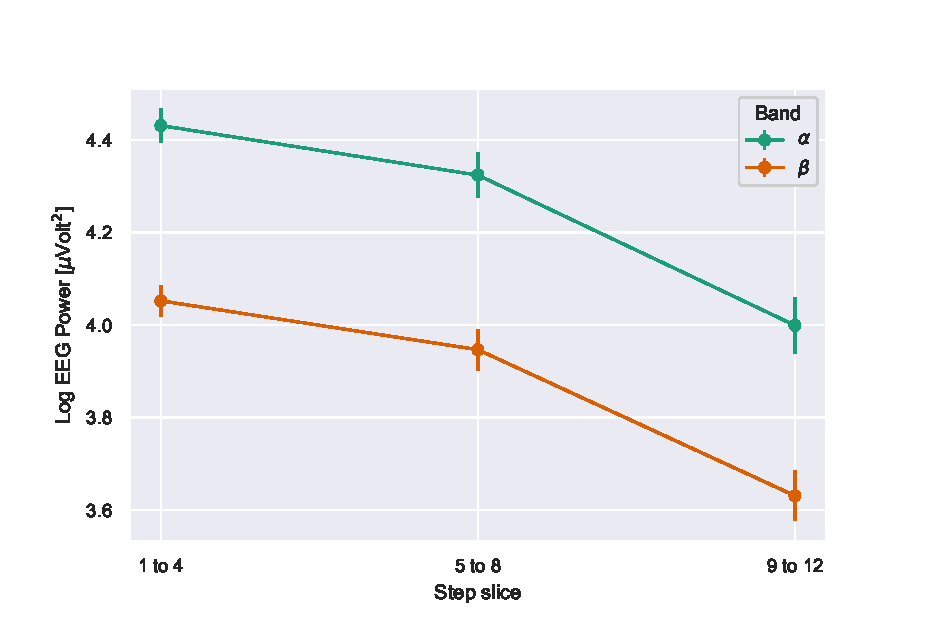
\includegraphics[width=.8\textwidth]{publications/2021ImpactDelayedResponse/Fig11.eps}
    \caption{Log of the average \gls{EEG} Power for alpha and beta bands per step slice. Error bars indicate \gls{SEM}.}\label{paper:olguinmunoz2021impact:fig:logeegpow:slices}
\end{figure}

\subsection{\acs{GSR} and Heart Rate}
The measure of \gls{GSR} was the log of total amplitude in the signal.
To control for effects of block length (steps~\( \times \)~delay) and the slow-down in execution time at longer delays, \gls{GSR} data were normalized by the temporal duration of the block.
Due to sensor failure and the elimination of one subject with extreme values of \gls{GSR} amplitude using the same rule as for \gls{EEG}, the analysis comprised 34 participants.
No systematic trend due to delay or block length was observed.
In addition, the same analysis of slice position within block length as was performed for the \gls{EEG} revealed no effects, indicating that \gls{GSR} was stable across step positions within a block.

Heart rate averaged \num{90.2}~\gls{BPM} and showed no trend related to the experimental variables of delay and block length.
The same was true of the variability in \gls{BPM} (average standard deviation across conditions was \num{20.3}).

The absence of systematic trends in both these results is interesting in the context of our initial suggestions of potential mechanisms relating delay in the application to human behavior.
In section \cref{paper:olguinmunoz2021impact:ssec:potentialmechs} we proposed that emotional arousal during the execution of the task was a potential explanation for the effects observed in the human.
However, these results seem to refute this hypothesis, and will be further discussed in \cref{paper:olguinmunoz2021impact:sec:discussion}.

\subsection{Individual Difference Analysis}

The \gls{BFI} and \gls{ITQ} were combined with outcome variables in an analysis of individual differences.
Given the previous results, we initially considered the following outcome variables:
\begin{itemize}
    \item execution time in the most demanding block (length 12, delay \SI{3.0}{\second}); 
    \item total of alpha and beta bands \gls{EEG} in the first four steps at all lengths (``Slice 1'');
    \item average heart rate;
    \item and average log \gls{GSR}.\@
\end{itemize}

Although the heart rate and \gls{GSR} data had produced no significant effects in the analysis of experimental variables, they could in principle correlate with experimental outcomes across individuals.
A \gls{PCA} on a subset of these variables, shown in \cref{paper:olguinmunoz2021impact:tab:pca}, was ultimately conducted on the 28 participants for which there was \gls{EEG} data.
Three of the personality measures were excluded after initial analyses indicated significant correlations among neuroticism, openness, agreeableness, and extroversion.
Neuroticism (with poles of sensitivity and security) was selected as most relevant to the issue of response to system delay and was included along with conscientiousness.
\gls{GSR} was used in a subsidiary analysis, because only 25 participants had both \gls{EEG} and \gls{GSR} measures that were reliable.

\begin{table}[h]
  \centering
  \caption{Principal Component Analysis}\label{paper:olguinmunoz2021impact:tab:pca}
  \begin{subtable}[h]{\textwidth}
    \centering
    \caption{Main components identified.}
    \setlength{\tabcolsep}{0pt} % let TeX compute the intercolumn space
    \begin{tabular*}{\columnwidth}{@{\extracolsep{\fill}\quad}lrrr@{}}
      \toprule
      \textbf{Factor} & \textbf{Comp. 1} & \textbf{Comp. 2} & \textbf{Comp. 3} \\
      \midrule
      \gls{BFI} Conscientiousness                  & \textcolor{lightgray}{\( -0.022 \)} &                         \( 0.668 \) & \textcolor{lightgray}{\( -0.481 \)} \\
      \gls{BFI} Neuroticism                        &                         \( 0.600 \) &                        \( -0.678 \) & \textcolor{lightgray}{\( -0.118 \)} \\
      \gls{ITQ} Focus                              &                         \( 0.678 \) &  \textcolor{lightgray}{\( 0.203 \)} &                         \( 0.504 \) \\
      \gls{ITQ} Involvement                        &                         \( 0.573 \) &                         \( 0.540 \) &  \textcolor{lightgray}{\( 0.417 \)} \\
      Exec. Time (delay 3.0 s, length 12)    &                         \( 0.758 \) & \textcolor{lightgray}{\( -0.178 \)} & \textcolor{lightgray}{\( -0.348 \)} \\
      Log \gls{EEG} power \( \alpha + \beta \) Slice 1 & \textcolor{lightgray}{\( -0.436 \)} & \textcolor{lightgray}{\( -0.251 \)} &                         \( 0.589 \) \\
      \bottomrule
    \end{tabular*}
  \end{subtable}
  \newline
  \medskip
  \newline
  \begin{subtable}[h]{\textwidth}
    \centering
    \caption{Percentages of variance explained by the components.}
    \begin{tabular*}{\columnwidth}{@{\extracolsep{\fill}\quad}lrrrr@{}}
      \toprule
      {} & \textbf{Comp. 1} & \textbf{Comp. 2} & \textbf{Comp. 3} & \textbf{Total} \\
      \midrule
      Explained Variance & \SI{31.88}{\percent} & \SI{22.22}{\percent} & \SI{19.03}{\percent} & \SI{73.13}{\percent} \\
      \bottomrule
    \end{tabular*}
  \end{subtable}
\end{table}

The \gls{PCA} produced three components that accounted for \SI{73.13}{\percent} of the variance in the six factors considered.
Component 1 included neuroticism, both \gls{ITQ} scores, and execution time, indicating that more sensitive and immersed individuals tended to slow their responses under extended delay.
Component 2 included conscientiousness and the absence of neuroticism along with immersive involvement, indicating that efficient and secure participants tended to be more involved.
The third component had positive loadings on \gls{EEG} in Slice 1 (first four steps of a block) and the focus component of the \gls{ITQ}.\@
An additional analysis including heart rate added a component but improved the \gls{PCA} fit by only \SI{4.5}{\percent}, indicating that any variability in this measure across individuals is unrelated to personality, immersiveness, or outcome.
A further analysis including \gls{GSR} produced a solution in which \gls{GSR} loaded with the first component, along with execution time.
% A further analysis including \gls{GSR} again produced a three-component solution, in which \gls{GSR} loaded with the first component (execution time, sensitivity, immersion).

\cref{paper:olguinmunoz2021impact:fig:neuro:exectime:reg} shows the correlation between neuroticism and execution time for the block with extreme values of length (12 steps) and delay (\SI{3.0}{\second}), for the full set of 40 participants.
It confirms the relationship indicated by the first component in the \gls{PCA} using the smaller sample of 28 participants; that is, higher neuroticism is associated with more responsiveness to delay.

\begin{figure}[h]
    \centering
    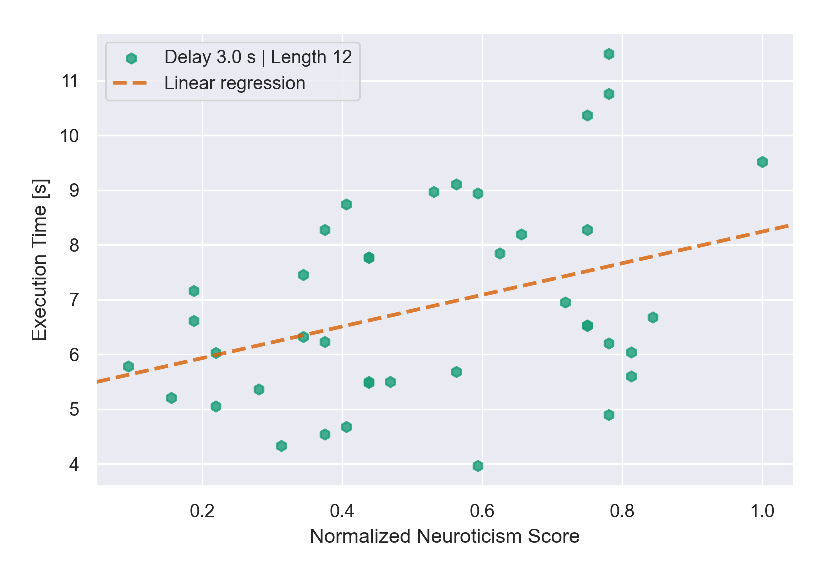
\includegraphics[width=.8\textwidth]{publications/2021ImpactDelayedResponse/Fig12.eps}
    \caption{Correlation between neuroticism score of participants and their execution time in the longest block at the longest delay.
    Pearson correlation coefficient \( r = .40 \); 2-tailed \( p = .01 \).}
    \label{paper:olguinmunoz2021impact:fig:neuro:exectime:reg}
\end{figure}

On the whole, these results suggest that individual differences in widely accepted personality variables and immersive tendencies moderate the response to delay.
This fact could have practical implications in the future.
It could, for instance, provide a tunable parameter for eventual models aiming to emulate human interaction with a \gls{WCA}.\@
In addition, physiological measures of heart rate and \gls{EEG} appear not to be direct indicators of  behavioral response to delay, although \gls{GSR} may be more promising in this regard.

\section{Discussion}\label{paper:olguinmunoz2021impact:sec:discussion}

% First summarize the main findings
We start our discussion with the main results of our experimentation presented in the previous section:

\begin{itemize}
  \item Firstly, and perhaps most importantly, we find that a system slow-down induces an \textit{additional} behavioral slow-down.
  That is, as system responsiveness decreases, our data indicates that users significantly slow-down in their execution of the task.
  This slow-down scales with the decrease in responsiveness; compared to the no-delay case, participants were on average \SI{12}{\percent} slower at \SI{1.65}{\second} delay and \SI{26}{\percent} at \SI{3.0}{\second} delay.
  Moreover, there is a temporal component to this effect; users become progressively slower the more time passes with reduced system responsiveness.

  \item Secondly, we find that the effects of behavioral slow-down due to impaired system responsiveness \emph{remain} for at least a few steps after system responsiveness improves.
  This is evidenced by the longer per-step-execution times of the first four steps of blocks immediately following a high-delay block, as pictured in \cref{paper:olguinmunoz2021impact:fig:exectime:transition}.
  The question of whether any lingering effect can be measured after these four steps remains open.

  \item Thirdly, we evidence a speed-up in execution time over a series of steps; that is, subjects get faster at performing steps as the task progresses.
  However, the strength of this effect decreases as delay increases.
  Whereas for blocks without delay users performed the last four steps of a 12-step block on average \SI{36}{\percent} faster than the first four, at the maximum delay this effect practically disappears.

  \item Fourthly, in terms of inter-subject differences, \gls{PCA} revealed three main factors governing users' response to delay.
  The first factor represents sensitivity to delay as moderated by the ``Big Five'' personality trait of neuroticism and both measures of immersion: focus and involvement.
  Factor two and three represent dedication to the task as opposed to delay intolerance and reflect variables related to attentiveness, respectively.
  In simple terms, these results suggest that the effects of delay are most potent in individuals who are sensitive and involved in the task.
  The findings appear selective to cognitive assistance tasks like the present ones, inasmuch as the same measures did not correlate with outcomes in other computer-intensive environments such as immersive VR~\cite{quesnel2018are}.
  These correlations are also consistent with previous findings indicating that individuals scoring high in neuroticism tend to be intolerant to delayed reward~\cite{hirsh2008delay}.
\end{itemize}

A central question therefore arises: to which physio- and psychological mechanisms can these findings, most importantly the substantial slow-down in task execution, be attributed?

In \cref{sec:background}, we initially considered the possibility that delays might produce negative emotional reactions.
These could in turn elicit generalized arousal.
We also postulated that adapting to delay might progressively deplete cognitive resources in users.
However, the present data provide relatively little support for these alternatives, in that the predicted measures did not produce the expected statistical trends.
Specifically, physiological measures of \gls{GSR} and heart rate failed to show evidence of differential arousal under long vs.\ short delays, and speed-induced errors and non-completions predicted by resource depletion were not observed.
The acceleration data further did not indicate that extended delay significantly increases erratic movement.
% physiological measures of \gls{GSR} and HR failed to show evidence of differential arousal under long vs.\ short delays, and speed-induced errors and non-completions predicted by resource depletion were not observed.
% The acceleration data further do not indicate that extended delay increases erratic movement.
To the contrary, the data suggest this effect results from a delay in movement after an instruction is introduced.
That is, users fail to capitalize on the new information as quickly as they could.
Thus, contrary to our preliminary postulations, behavioral effects seem to arise from impaired cognitive control mechanisms, and not from emotion or resource depletion.
We hypothesize that the effects of feedback latency can best be understood as changes in the use of a cognitive plan.
As was described in \cref{paper:olguinmunoz2021impact:sec:experimentaldesign,paper:olguinmunoz2021impact:fig:lego:hierarchical}, complex cognitive and motor tasks have been modeled as the unfolding of a hierarchy of command, from high-level plans to physical output.
Long system latencies, we propose, disrupt the automating of such a plan, instead relegating it to attention-based control at the step-by-step level that is easily diverted.
This also provides a possible explanation for the lingering effects of delay after an acceptable system responsiveness is restored, as users needs time re-adjust and re-automate their cognitive plans.

As to the applicability of our findings to other applications, it must be noted that these results pertain to a specific class of applications, namely step-based task-guidance \gls{WCA}.\@
However, we would expect our findings to extend to similar applications, as long as they follow the same pattern of seamless interaction --- i.e.\ such that the user does not need explicitly interact with the application to advance the state.

The results here presented provide a number of possible implications for \gls{WCA} system design and optimization, both for single and multi-application flows.

\begin{itemize}

  \item Due to the behavioral slow-down in users, even short-term reductions in responsiveness will lead to significantly extended application lifetimes.
  This has direct implications for resource and power consumption.
  
  \item The fact that the adverse effects of delay on users do not immediately disappear as the system returns to a high-responsive state could have unconventional consequences for resource allocation.
  This is of particular importance, for instance, for cases where the user may be able to finish the task before these effects subside.
  In such cases, the limited potential gains might not justify diverting valuable system resources to the impaired application.

  \item In multi-user environments, the time dependency of user slow-down effects mean that fair degradation of system responsiveness across applications may not ultimately be beneficial to the system as a whole.
  Take for instance two applications on the same system which negatively interfere with each other. 
  The longer they interfere with each other, the longer their respective lifetimes are going to be, which in turn causes them to interfere even longer, potentially entering a positive feedback loop. 
  In such a case, prioritizing one over the other rather than trying to improve responsiveness for both might lead to resources being freed up faster system-wide.

  \item Based on our findings relating individual differences between users and their sensitivity to delays, it might also be possible to extrapolate user characteristics from measured execution times.
  This could prove a valuable tool for load balancing, for instance by prioritizing resource allocation to users with a higher sensitivity to system-state degradation.
  However, this remains an open challenge.

\end{itemize}

To wrap up, we believe the present data provide novel and unexpected insights for the understanding and optimizing of \gls{WCA} deployments.
Although more subtle than expected, and in some cases somewhat counterintuitive, these insights represent a valuable tool to tackle inefficiencies in these systems.
Moreover, we also argue these findings represent a first step towards a full-fledged understanding of the relationship between application responsiveness and human behavior.
More research in this area will surely uncover more complex and interesting behaviors.
Finally, we believe the data provide parameters that can usefully be integrated into cognitive models of \gls{WCA} that might be constructed under existing architectures like ACT-R.
These same parameters could be used to modulate the timing and generation of inputs in trace-based workload generation tools such as the EdgeDroid platform~\cite{olguinmunoz2018demoscaling,olguinmunoz2019edgedroid}, allowing the tool to use the same trace to generate workloads for a multitude of different user profiles.

\section{Conclusion}\label{paper:olguinmunoz2021impact:sec:conclusion}

In this paper, we presented the results of a study on the physiological and behavioral reactions of users of \gls{WCA} to delays in the application pipeline.
Our ultimate aim was to identify and categorize the ways in which humans react to low system responsiveness in step-based cognitive assistance systems.

We approached this in an experimental manner, by having participants interact with an instrumented \gls{WCA} setup, and found that delay appears to affect the cognitive plan of users, preventing them from automating the task they are performing.
The results show that user interactions in a \gls{WCA} slow down in the presence of delays in the application pipeline.
When system responsiveness is high, the user responds quickly; when it is low, the user slows down.
This was evidenced by an increase in task execution times, even after accounting for the artificially introduced delays, as well as accelerometer data from participants wrists.
Additionally, we found that the strength of this effect is modulated by individual differences between subjects.

These results are interesting as they open up hitherto unexplored opportunities for the design, optimization and benchmarking of \gls{WCA} systems.
In this context, we believe there are two direct and important next steps to be performed.
The first of these relates to the implications for system optimization and resource allocation discussed in \cref{paper:olguinmunoz2021impact:sec:discussion}.
We believe these need to be implemented, tested and validated in real setups.
In particular, we identify two of these implications to be prime candidates for their own experimental studies.
One, our postulation that in cases where an impaired application is close to finishing, diverting resources to it might not be the most optimal course of action; and two, the possibility that ``fair'' degradation of system responsiveness across applications may be, in some cases, undesirable.
Both of these questions could be answered with straightforward setups.

The second step corresponds to the extension of existing tools for \gls{WCA} benchmarking with the findings presented in this paper.
These tools are of great usefulness for the study of \gls{WCA} systems, as they allow for automated large-scale testing without having to resort to human users.
However, they are still somewhat simplistic and unrealistic in their workload generation schemes.
Incorporating the results presented here would allow for much more realistic workloads.
For instance, our findings relating to the effects of delay on execution times could be directly adapted to modulate timings in the input stream.
Another example would be employing the results linking neuroticism to a heightened sensibility for delays to provide a ``tuning knob'' for the user models in these workload generation schemes.
Extending and perfecting these tools will allow for much more realistic benchmarking and testing of \gls{WCA} systems, providing data of significantly better quality and ultimately leading to faster improvement, optimization and adoption of these systems.

\begin{acks}
  This research was supported in part by the \gls{SSF} under grant \texttt{ITM17-0246} (ExPECA) and the \gls{NSF} under grant number \texttt{CNS-1518865}.
  Any opinions, findings, conclusions or recommendations expressed in this material are those of the authors and do not necessarily reflect the view(s) of their employers or funding sources.
\end{acks}

\thesispaper{CLEAVE}{olguinmunoz2022cleave}

\begin{abstract}
    As the number of cyber-physical systems rises, it becomes increasingly crucial to study \glspl{NCS} combining control communication co-design. This nature of \glspl{NCS} has led to task-specific approaches to research, creating a dearth of generalizable, repeatable, and scalable experimentation. Further, with the advent of edge computing solutions, it is of paramount importance to explore its relevance in such applications. In this work, we present \gls{CLEAVE}, a novel, completely software-based framework for repeatable and scalable experimentation in edge native \glspl{NCS}.
    Our approach is based on the emulation of physical plants communicating over a real network with software-based controllers.
    \gls{CLEAVE} is designed and built for the edge, using Python3 and with full compatibility with industry-standard containerization solutions.
    Although designed for single-loop emulations, the flexibility afforded by the aforementioned characteristics allow our framework to be adapted to a multitude of complex scenarios.

    We validate \gls{CLEAVE} using an initial implementation of an inverted pendulum \gls{NCS}.
    Our results showcase the utility of the tool as a repeatable, extensible, and scalable solution to \gls{NCS} performance evaluation and benchmarking on the Edge.
\end{abstract}
\section{Introduction}\label{paper:olguinmunoz2022cleave:intro}

The number and applications of \glspl{CPS}~\cite{rajkumar2010cyber} --- i.e.\ systems in which a real, physical mechanism is controlled by a computer --- have exploded in recent years.
However, this rapid increase in adoption has mostly been limited to industrial contexts.
Although \glspl{CPS} present huge opportunities for all facets of society, they have yet to reach our daily lives in any relevant scale due to their stringent operational requirements.
This is about to change, however, as with the advent of novel wireless communication technologies as well as networking paradigms, such as cellular 5G and edge computing~\cite{satyanarayanan2017emergence}, consumer-grade \glspl{CPS} will be made possible.
These technologies meet two key requirements of \glspl{CPS}: real-time capabilities (through extremely low end-to-end latencies), and context- and locality-awareness, and will most likely become the backbone of \gls{CPS} in the future.

\glspl{NCS}~\cite{gupta2010networked}, a type of \gls{CPS} wherein multiple networked actuators and sensors form a part of the same automatic control system will benefit from the adoption of these technologies.
Depending on the physical system being controlled, \glspl{NCS} can have stringent timing and reliability requirements for communication that conventional cloud paradigms and cellular networks cannot meet~\cite{wan2020efficient}.
This necessitates sophisticated tools for the performance evaluation of future system architectures, as well as novel NCS design paradigm.

%Due to their potential advantages for industrial and commercial settings, there exist works~\cite{Zhang2016Survey} dedicated to the modelling and performance characterization of \glspl{NCS}, improving NCSs by distributing control functions across networks, facilitating centralized coordination, control, and monitoring.

One the one hand, related literature in \glspl{NCS} leverages to a large extent theoretical models, at the price of being able to capture networked systems effects only on a coarse level.
%follows a theoretical approach, and only a small fraction of it deals with experimental studies.
On the other, there exist several approaches when considering experimental methodologies. 
%A number of works concerning \glspl{NCS} deal with experimental studies.
%\glspl{NCS} have an inherently inter-domain nature intertwining knowledge from the fields of communications, computing, and control theory in ways that cannot be studied in isolation, leading to various different approaches to such studies.
One such approach uses setups in which the complete system is built on top of real hardware.
This approach is employed in the works of Baumann \emph{et al.}~\cite{baumann2018evaluating} and Cuenca \emph{et al.}~\cite{cuenca2019periodic}; in both of these, the authors implement their approach on physical testbeds.
Conversely, other studies choose to instead use completely \emph{simulated} \gls{NCS} setups.
The authors in\ \cite{ma2019optimal} have opted for such an approach.
These studies often employ combinations of physical and network simulation tools trying to capture the complex dynamics of \glspl{NCS}.
Finally, some experimental studies instead employ \emph{virtualized} approaches, in which either
\begin{inlineenum}[itemjoin={{; }}, itemjoin*={{; or }}]
    \item a real network interacts with a simulated or emulated control system~\cite{wang2020inverter}
    \item a simulated network interacts with a real control system~\cite{natale2004inverted}.
\end{inlineenum}

As evidenced above, experimental research in \glspl{NCS} includes varied heterogeneous hardware and software platforms, methodologies and key performance indicators.
This, in turn, leads to hardware, software, and methodology fragmentation, as different studies tend to prefer approaches more favored in their respective communities.
Furthermore, existing studies tend to focus on individual aspects and components of a system, thus producing results which do not provide a complete image of the \gls{NCS}.
This has caused a gap in knowledge pertaining to the reproducibility and comparison of experimental studies on these systems.

Zoppi \emph{et al.}~\cite{zoppi2020ncsbench} made the first (and to the best of our knowledge, the only) attempt at tackling this challenge in their work.
In their work, they proposed a platform called NCSBench, to be used for reproducible benchmarking in NCS.\ 
Their methodology utilizes joint knowledge of control, computation, and communication. 
In their work various architectural elements and the corresponding delays associated with the NCS are modelled. 
Multiple experimental parameters and certain observable key performance indicators are defined and utilized in the implementation. 
This work however utilizes a physical LEGO\textregistered{}\ Mindstorms EV3 Core Set\texttrademark{}\  based plant for the implementation, preventing instantaneous changes in plant characteristics and component parametrizations.
Furthermore, relying on physical objects like an inverted pendulum limits scalability of the experimentation in practice. 

We overcome this issue by proposing a completely virtual plant allowing for unparalleled flexibility in changing the plant model and characteristic features of the experiments.
In this paper, we present the first fully-software-based framework for scalable and repeatable benchmarking of edge-native \gls{NCS}.
As edge computing begins being adopted by industry, more and more variations have begun to appear in literature.
``Near'', ``far'', ``core'', and ``telco'' edge describe variations of the original concept and are becoming ubiquitous in new research.
While the core idea of edge computing is widely accepted as fundamental for pervasive \glspl{NCS} in general, understanding the strengths and weaknesses of such different edge concepts is of paramount importance.

Our framework, \gls{CLEAVE}, aims to simplify the repeatable and scalable benchmarking of such systems.
It is fully virtualized, inspired by our previous work on benchmarking human-in-the-loop applications on the edge~\cite{olguinmunoz2019edgedroid}.
The tool consists of a benchmarking framework and software development kit for the development of emulated physical systems and softwarized controllers.
These virtual \glspl{NCS} can then be deployed on real networks for reparametrizable, repeatable, and reproducible benchmarking of the complete system.

\gls{CLEAVE} is built using \emph{Python 3.8}, making it highly extensible and able to harness the multitude of already existing user libraries.
It is furthermore compatible with container technologies such as \emph{Docker}\footnote{Docker Engine: \url{https://www.docker.com/}}, making it suitable for automated deployment, scaling, and benchmarking on industry-standard edge setups using container orchestration solutions.

The rest of this paper is structured as follows.
\cref{paper:olguinmunoz2022cleave:approach} presents the design principles and implementation of the framework.
In \cref{paper:olguinmunoz2022cleave:experiments}, we present a use case scenario which validates the utility, flexibility, and repeatability of \gls{CLEAVE}.
Finally, in \cref{paper:olguinmunoz2022cleave:conclusion} we conclude this work.

\section{The \gls{CLEAVE} framework}\label{sec:approach}

In this section, we detail our \gls{CLEAVE} framework for the performance evaluation of \glspl{NCS}, with an emphasis on edge deployments.
Our design follows a virtualized emulation approach; providing a framework for the real-time \emph{emulation} of physical control systems and the easy implementation of softwarized controllers interacting with \emph{real} networks.
\gls{CLEAVE} is thus a platform with an easy-to-use \gls{API} on which a multitude of \gls{NCS} types can be emulated.
This allows for great flexibility, as the core components of the \gls{NCS} can be switched out while maintaining the realism of the network, the most complex and limiting component of edge \glspl{NCS}.

The framework is distributed as \emph{free and open-source} software through the \emph{GitHub} organization of the \emph{KTH ExPECA} research group\footnote{\url{https://github.com/KTH-EXPECA/CLEAVE}}.
We also plan to provide a library of \gls{NCS} implementations, making the tool even more accessible.

\subsection{Design and Implementation}\label{sec:design}

The design of \gls{CLEAVE} attempts to target a broad a set of different control systems as possible, and tries to minimize the number of assumptions made about the systems implemented on top of the framework.
These are:
\begin{enumerate}
    \item Controllers can be stateful or stateless, but they exclusively control a single plant.
    \item Plants and controllers interact in a ``request-response'' manner.
    We currently don't support setups in which the controller generates an actuation command without there first being a request from the plant.
    \item Controller and plant communicate over a TCP/IP network.
    \item The physical state behavior of the plant can be implemented in a discrete-time manner.
    \item Values associated to sensors and actuators can be represented as integers, floating point numbers, booleans, or sequences of bytes.
    \item A plant has zero or more sensors attached to it, with potentially different sampling rates.
    \item A plant has zero or more actuators attached to it.
\end{enumerate}

\cref{fig:cleave:ncs:struct} shows an overview of the conceptual structure and operation of \gls{CLEAVE}.
The \emph{State} implements the discrete-time behavior of the Plant.
At the beginning of each time-step, actuated variables in the \emph{State} are updated with values obtained from the \emph{Actuator} objects.
Conversely, at the end of each time-step, sensed variables are sampled and used to update values associated with \emph{Sensor} objects.
These values are processed at the \emph{Sensors} (e.g.\ to add noise) before being sent over the network to the \emph{Controller}.
The \emph{Controller} calculates actuation values and updates the \emph{Actuators} over the network.
Finally, the \emph{Actuators} process the actuation values and hold the results until they are read at the next time-step.

Implementation-wise, \gls{CLEAVE} is built on top of the well-established and stable \emph{Twisted}\footnote{\url{https://twistedmatrix.com}} asynchronous programming and networking framework.
The aforementioned core components (\emph{State}, \emph{Controller}, \emph{Sensors}, and \emph{Actuators}) are provided as \glspl{ABC} with core functionality that users must extend for their specific use cases and \glspl{NCS}.
The framework makes no assumptions about the inner workings of the user implementations of these classes other than the interfaces they expose.
Users are therefore free to implement arbitrarily complex functionality in these components.
On the other hand, \gls{CLEAVE} handles network communication and metric collection autonomously; users only need to select the desired transport protocol (we do however provide an \gls{API} for extending the available transports).

Below we present a brief overview of the design and implementation of the core components.

%\begin{description}[style=nextline]
%\begin{itemize}
\textbf{State Base Class}:
\gls{ABC} with an abstract method
\mintinline{python}{advance()} which must be extended with the implementation of discrete-time emulation of the plant.
The \mintinline{python}{advance()} method is called by the framework periodically according to the configured emulation update rate, and should perform a single time-step of the discrete-time emulation.
Two optionally extensible methods, \mintinline{python}{initialize()} and \mintinline{python}{shutdown()} are provided to implement single-fire set-up and tear-down procedures.

    % This class also provides functionality for the automatic tracking and updating of sensed and actuated values.
    % This is handled through special auxiliary classes, \emph{SensorVariable} and \emph{ActuatorVariable}, which when instantiated and assigned to an attribute of the \emph{State} allow the framework to track and modify them.

\textbf{Controller Base Class}:
Defines a single abstract method \mintinline{python}{process()}, taking a mapping of names to values corresponding to the sensed variables of the \emph{State}, and returning a similar mapping corresponding to the actuated variables.
This method is called by \gls{CLEAVE} in an event-based manner whenever samples are received from the plant side; however, we intend to extend this to time-interval-based approaches.

\textbf{Sensor Base Class}:
Implements processing of monitored stated variables before sending them over the network to the \emph{Controller}.
This base class must be initialized with a property name (corresponding to the monitored \emph{State} attribute) and a sampling rate in \si{\hertz}, and provides an abstract method \mintinline{python}{process_sample()} which must be extended with an implementation of the processing performed on each sample.

\textbf{Actuator Base Class}:
Performs the processing of actuation values obtained over the network from the \emph{Controller}.
It is initialized with a property name corresponding to the name of the actuated \emph{State} attribute, and provides two abstract methods which must be implemented by extending classes:
\begin{enumerate*}[itemjoin={{; }}, itemjoin*={{; and }}]
\item \mintinline{python}{set_value()}, called by the framework whenever a new value for the corresponding actuated attribute is received
\item \mintinline{python}{get_actuation()}, called on every time-step and must return a value to apply to the actuated attribute.
\end{enumerate*}
%\end{itemize}
%\end{description}


\subsection{Configuring and Executing \pgls{NCS}}

Once the core components for the emulation have been defined and implemented, they need to be registered with the framework.
This is done through Python scripts which define a number of required (and some optional) top-level variables, corresponding to emulation parameters such as the \emph{State}, \emph{Controller}, \emph{Sensor}, and \emph{Actuator} subclasses to use; the emulation update rate; the controller-side host and address; data output directories; \emph{et cetera}.
These Python configuration files are then provided as arguments to the \texttt{cleave} command line provided by the framework.
\gls{CLEAVE} imports and parses them, and then sets up and executes the emulation.

Although the core design of \gls{CLEAVE} follows a single-loop approach, multi-loop scenarios can be easily implemented through the combination of multiple \gls{CLEAVE} instances.
The framework does not make any assumptions about the individual components other than the signatures of methods on the \glspl{ABC} that must be extended and implemented.
Combined with the Python emulation configuration scripts, this makes development of more complex scenarios merely a matter of implementing the desired functionality within the framework itself.

\subsection{Current Implementations}

\begin{figure}
    \centering
    \includegraphics[width=.6\columnwidth]{publications/2022CLEAVE/images/inverted_pendulum.png}
    \caption{
        The 2D inverted pendulum system.
    }\label{fig:invpend}
\end{figure}

For the purpose of this work, we have used \gls{CLEAVE} to implement an emulated \emph{inverted pendulum} control loop (see \cref{fig:invpend}), the goal of which is to balance the vertically free-swinging pendulum by applying horizontal forces on the cart.
We have chosen this system as an initial benchmark for its relative simplicity as well as prevalence in the field of automatic control as one of the fundamental examples of linear control.

The inverted pendulum plant \emph{State} is implemented as a real-time discrete-time physical emulation using CLEAVE's API and a 2D physics library\footnote{Pymunk: \url{http://www.pymunk.org/en/latest/}}, updated at a constant \SI{120}{\hertz} (this value is configurable; in this case it corresponds to the maximum achievable stable rate on our available hardware).
\emph{Sensors} for the angle, position, angular velocity, and velocity of the \emph{State}, and an \emph{Actuator} for the horizontal force applied to the cart are implemented as ``perfect'', i.e.\ values are returned as-is, without any added noise.
For the controller side, a proportional-differential strategy is implemented using the framework \emph{Controller} API and the \emph{NumPy} numeric computation library\footnote{NumPy: \url{https://numpy.org/}}.
Plant and controller are then packaged into containers, for ease of orchestration and reparametrization, and to mimic real-world deployment.

A previously mentioned, we eventually plan to build an open library of emulated control loops.\footnote{%
    At the moment of writing, we are in the process of implementing \emph{model-predictive} as well as \emph{deep neural network} controllers for the inverted pendula plants.%
}
The inverted pendulum plant is merely a proof-of-concept, and \gls{CLEAVE} could be used to implement much more complex physical systems with even more stringent latency requirements.
For instance, the flexibility afforded by the choice of programming language and the abstractions detailed in \cref{sec:design}, allow for relatively straightforward emulation of autonomous drone dynamics.
Propeller dynamics could be implemented by \emph{Actuator} objects, gyroscopes by \emph{Sensors}, and the physical behavior of the plant could be modeled using a general purpose 3D physics engine (\emph{e.g.} the Panda3D\footnote{\url{https://docs.panda3d.org/1.10/python/programming/physics/builtin/index}{https://docs.panda3d.org/1.10/python/programming/physics/builtin/index}} engine).


\section{Use case validation}\label{sec:experiments}

In this section, we demonstrate the utility of \ac{CLEAVE} by walking readers through an example use case.
With this, we aim to showcase the ability of our framework to provide accurate and repeatable measurements of the performance of \acp{NCS} deployed on edge computing infrastructure.

We present the following use case scenario.
A simple \ac{NCS} consisting of an \emph{inverted pendulum} plant controlled by a \emph{proportional-differential} controller is to be deployed on an Edge server.
The connection between plant and server is over a WiFi (IEEE 802.11n) link.
Moreover, there are a number of video-streaming applications running concurrently on the Edge setup.

We believe this to be an interesting and representative use-case scenario for a number of reasons.
Firstly, the inverted pendulum is broadly used as a benchmark in control-system literature, see for instance\ \cite{Baumann2018LowPower} and\ \cite{Natale2004InvPendEthernet}.
A key reason for this is that such a relatively simplistic system allows for straightforward reparametrization to obtain varied system dynamics, which in turn makes a broader range of experiments possible.
Secondly, similar, albeit non-Edge-enabled, setups have been a reality in industry for almost two decades, as evidenced by\ \cite{Gupta2010NCSOverview}.
Thirdly, although real deployments would most assuredly employ mobile technologies due to the added benefits of mobility and range, the \acp{RTT} offered by these technologies are higher, or at best equal, those offered by WiFi.
4G, for instance, has average \acp{RTT} of around a few hundred milliseconds, which is orders of magnitude greater than the values measured in our scenario, and current 5G deployments offer \ac{RTT} values barely matching the sub-\SI{10}{\milli\second} values we obtain for WiFi.
Thus, we argue that using WiFi allows for more experimental freedom, as the system can be tweaked to obtain worse \acp{RTT} more akin to those of mobile technologies while still having the option to study best-case scenarios with very low-latencies.
Finally, video analytics is one of the main proposed use cases for edge computing~\cite{Ananthanarayanan2017Analytics,Yi2017Analytics,Wang2018Analytics}, and thus we foresee edge \ac{NCS} deployments being deployed in parallel with such applications in the future.
However, before deployment can become a reality, key questions such as: 
``what are the baseline requirements of the \ac{NCS}?''; ``what are the achievable best-case end-to-end latencies in the system?''; and
``how does the concurrent video-streaming traffic affect \ac{NCS} stability?'' need to be answered.

We attempt to study these questions using the experimental setup in \cref{fig:cleave:expsetup}.
\ac{CLEAVE} is deployed on a testbed consisting of \num{10} Raspberry Pi 4B  clients connected wirelessly to an IEEE 802.11n \ac{AP}.
Connected to the Ethernet backbone of this \ac{AP} is a general-purpose \verb|x86_64| desktop computer acting as a Cloudlet/Edge server.

% % Please add the following required packages to your document preamble:
% \usepackage{booktabs}
% \usepackage{graphicx}
\begin{table}[]
    \centering
    \caption{Hardware used in the experiments.}\label{tab:hardware}
    \resizebox{\columnwidth}{!}{%
    \begin{tabular}{@{}llrrrl@{}}
    \toprule
    \multicolumn{1}{c}{\textbf{}} &
      \multicolumn{1}{c}{\textbf{CPU}} &
      \multicolumn{1}{c}{\textbf{\begin{tabular}[c]{@{}c@{}}Freq\\ {[}\si{\giga\hertz}{]}\end{tabular}}} &
      \multicolumn{1}{c}{\textbf{\begin{tabular}[c]{@{}c@{}}Core\\ Count\end{tabular}}} &
      \multicolumn{1}{c}{\textbf{\begin{tabular}[c]{@{}c@{}}RAM\\ {[}\si{\giga\byte}{]}\end{tabular}}} &
      \multicolumn{1}{c}{\textbf{\begin{tabular}[c]{@{}c@{}}Operating\\ System\end{tabular}}} \\ \midrule
    \textbf{Cloudlet} &
      \begin{tabular}[c]{@{}l@{}}Intel\textregistered{} Core\texttrademark{}\\ i7-8700\end{tabular} &
      \num{3.2} &
      \num{6} &
      \num{32} &
      \begin{tabular}[c]{@{}l@{}}Ubuntu Server \\20.04 LTS \\Kernel v5.4.0\\\ \end{tabular} \\
    \textbf{Client} &
      \begin{tabular}[c]{@{}l@{}}Cortex-A72\\ (ARM v8)\end{tabular} &
      \num{2.0} &
      \num{4} &
      \num{8} &
      \begin{tabular}[c]{@{}l@{}}Ubuntu Server \\20.04 LTS \\Kernel v5.4.0\end{tabular} \\ \bottomrule
    \end{tabular}%
    }
\end{table}

\begin{figure}
    \centering
    \includegraphics[width=.95\columnwidth]{images/CLEAVE_experiment_setup}
    \caption{
        The setup used for our experimentation. 
        % Containerized versions of the core CLEAVE emulation components are deployed inside a Docker Swarm Overlay Network spanning \num{10} Raspberry Pi 4B clients connected to a single Cloudlet over an IEEE 802.11n \ac{AP}.
    }\label{fig:cleave:expsetup}
\end{figure}

The first step in our case study is to evaluate the baseline performance of the control system, both locally and over the network.
We configure \ac{CLEAVE} to run a single loop with both plant and controller co-located on the Edge server, and we also configure a separate setup with an identical loop executed over the wireless link.
For both of these setups, we execute a series of scenarios varying:
\begin{enumerate*}[itemjoin={{; }}, itemjoin*={{; and }}]
    \item the sampling rate of the Plant state, setting it to \SIlist[list-final-separator={, or }]{5;10;20;40;60}{\hertz}
    \item the responsiveness of the Controller, adding fixed delays of \SIlist[list-final-separator={, or }]{0;25;50}{\milli\second} after the processing of each sample.
\end{enumerate*}

We run repeated executions of each combination of these parameters at least \num{10} times, for both the networked and ``local-only'' setups.
Each execution lasts for \SI{5}{\minute}, during which we collect detailed data on both the state of the controlled system as well as on the data sent over the network.
After the initial \num{10} runs, we identify that setups with sampling rates of \SIlist{5;10}{\hertz} were consistently too unstable to consider, and disregard them in further analyses.
We further note that setups with \SI{0}{\milli\second} additional delay are always stable and thus also disregard them.
Remaining setups, i.e.\ sampling rates \( \geq \) \SI{20}{\hertz} and artificial delays \( \geq \) \SI{25}{\milli\second}, are repeated an additional \num{20} times for better statistical significance.

This repeated experimentation and data collection while ``zooming in'' on particular setups is facilitated by \ac{CLEAVE}'s design.
Scenarios are executed automatically in batches using a simple Python script which interacts with Docker through the widely adopted \emph{docker-py}\footnote{Docker SDK for Python: \url{https://docker-py.readthedocs.io/en/stable/}} library.
This is \ac{CLEAVE}'s first advantage over existing frameworks; it is designed with cloud and edge technology and paradigms in mind, making integration with existing systems convenient.

\begin{figure}[t]
    \centering
    \begin{subfigure}[t]{\columnwidth}
        \centering
        \includegraphics[width=\textwidth]{fixed_single_loop_toppled}
        \caption{Fraction of toppled plants.}\label{fig:single:topple}
    \end{subfigure}\\
    \begin{subfigure}[t]{\columnwidth}
        \centering
        \includegraphics[width=\textwidth]{fixed_single_loop_rms}
        \caption{Mean angle \acs*{RMS}; red line indicates \( y = 180 \).}\label{fig:single:rms}
    \end{subfigure}\\
    \begin{subfigure}[t]{\columnwidth}
        \centering
        \includegraphics[width=\textwidth]{fixed_single_loop_rtts}
        \caption{
            Mean \acsp*{RTT}.
        }\label{fig:single:rtt}
    \end{subfigure}%
    \caption[caption]{
        Baseline results.
        Error bars indicate \SI{95}{\percent} \acp{CI}.
        }%
    \label{fig:single}
\end{figure}

\cref{fig:single} shows a summary of the results relating to the single-loop scenarios:
\cref{fig:single:topple} shows the fraction of plants that toppled in each scenario, and \cref{fig:single:rms} shows the average \ac{RMS} for the absolute pendula angles.
\cref{fig:single:rtt} shows average latency due to network and processing (excluding synthetic delays) for both single-loop scenarios.
Packet losses were below \SI{0.2}{\percent} for all parametrizations of the single-loop scenario over the network, and \SI{0}{\percent} for all parametrizations of the local-only setup.

As expected, higher sampling rates tend to correlate with better quality of control; at higher sampling rates the system was able to reach stability at higher \acp{RTT}.
These initial results already hint at interesting consequences for such an edge-bound \ac{NCS} deployment.
For instance, it is clear from \cref{fig:single:topple,fig:single:rms} that network delays can, to a certain extent, be compensated for by increasing the sampling rate of the system.
A corollary of this is, conversely, that at lower network latencies \acp{NCS} are able to stabilize at lower sampling rates.
Adaptive sampling might thus be a viable method for optimizing resource utilization.

Once baselines for single loops in the use case scenario have been established, we can proceed to studying the interaction between the \acp{NCS} and the video-streaming applications.
We deploy \num{6} control loops on the experimental setup depicted in \cref{fig:cleave:expsetup}.
On the remaining \num{4} clients we run the \emph{iperf3}\footnote{iperf3: \url{https://iperf.fr/}} traffic load generator, each generating \SI[per-mode=symbol]{6.5}{\mega\bit\per\second} of uplink \ac{UDP} traffic.
This emulates the load generated on the network by \SI{1080}{p} Full-HD video streaming, originating from the clients and terminating in the cloudlet.
Based on the baseline results, we execute setups with \ac{NCS} plant sampling rates of \SIlist{20;40;60}{\hertz}.
Each sampling rate configuration is run for \SI{5}{\minute}, and then repeated \num{30} times to obtain statistical significance.
Once again, repetitions of this scenario are executed automatically in batches using a simple Python script and \emph{docker-py}.

\begin{figure}[t]
    \centering
    \begin{subfigure}[h]{.22\textwidth}
        \centering
        \includegraphics[width=\textwidth]{fixed_video_topple_frac}
        \caption{Toppled plants.}\label{fig:video:toppled}
    \end{subfigure}%
    \hfill%
    \begin{subfigure}[h]{.22\textwidth}
        \centering
        \includegraphics[width=\textwidth]{fixed_video_angle_rms}
        \caption{Angle \ac{RMS}.}\label{fig:video:rms}
    \end{subfigure}\\
    \begin{subfigure}[h]{.22\textwidth}
        \centering
        \includegraphics[width=\textwidth]{fixed_video_drop_frac}
        \caption{Packet losses.}\label{fig:video:drop}
    \end{subfigure}%
    \hfill%
    \begin{subfigure}[h]{.22\textwidth}
        \centering
        \includegraphics[width=\textwidth]{fixed_video_rtt}
        \caption{\acsp{RTT}.}\label{fig:video:rtt}
    \end{subfigure}%
    \caption{
        Multi-loop, resource-constrained setup results.
        Error bars indicate \SI{95}{\percent} \acp{CI} in all plots.
    }\label{fig:video:results}
\end{figure}

\cref{fig:video:results} shows a summary of the results obtained.
\cref{fig:video:toppled} shows the fraction of repetitions of each setup in which \emph{at least} one plant failed to maintain stability and toppled.
\cref{fig:video:rms} shows the \ac{RMS} for the pendulum angles for each setup, only considering data from plants that did not topple.
\cref{fig:video:drop} shows the fraction of \ac{UDP} datagrams dropped, averaged over all plants and repetitions per setup.
\cref{fig:video:rtt} shows the measured end-to-end plant-side \ac{RTT}, averaged over all plants and repetitions per setup.

These results are interesting in their counter-intuitiveness compared to the single-loop baseline results.
While the baselines might lead us to think that higher sampling rates are always better for the stability of control systems, \cref{fig:video:toppled,fig:video:rms} show this not to be the case for \ac{NCS} in resource-constrained scenarios.
\SI{60}{\hertz} was the least stable configuration, with at least one pendulum toppling in around \SI{16}{\percent} of the repetitions, and mean pendulum angle \ac{RMS} circa \num{3} times that of the \SI{40}{\hertz} scenario.
\SI{40}{\hertz} was in turn the second worst configuration --- although it presented no toppled pendula, average angle \ac{RMS} doubled that of the \SI{20}{\hertz} setup.

\cref{fig:video:drop,fig:video:rtt} explains these behaviors.
Whereas both the \SIlist{20;40}{\hertz} setups show losses well below \SI{5}{\percent}, the \SI{60}{\hertz} scenario shows an average of around \SI{13}{\percent} of datagrams lost.
The differences in \acp{RTT} results are equally telling; \acp{RTT} for the \SI{60}{\hertz} setup were on average approx.\ \num{3} times those for the \SIlist{20;40}{\hertz} setups.
These results stem from the contention for network resources, and hint at important trade-offs system designers will have to take into consideration when designing and developing \acp{NCS} for deployment on the Edge.
The Edge will be \emph{multi-tenant} and \emph{multi-instance}. 
\ac{NCS} deployments will have to be designed with shared resources in mind, and given the complexity of these systems, experimental tools like \ac{CLEAVE} will be key for their succesful adoption and massification.

\section{Conclusion}\label{sec:conclusion}

The issue of repeatable and scalable benchmarks has been largely glossed over in \ac{NCS} literature, as existing experimental research studies tend to implement \emph{ad-hoc} solutions.

In this work, we aimed to tackle this issue through a fully software-based framework for repeatable, reproducible, and easily scalable \ac{NCS} benchmarking with a particular focus on edge deployment.
We argue our approach, \ac{CLEAVE}, embodies a better solution than previous work for a number of reasons:
\begin{enumerate}
    \item Compared to fully physical approaches, such as those used in\ \cite{Baumann2018LowPower} and\ \cite{Cuenca2019UAV}, our approach allows for greater flexibility and scalability.
    The aforementioned approaches rely on specialized and sometimes entirely custom-built physical platforms, and although flexible and cheap approaches such as Zoppi \emph{et al.'s} --- which uses a LEGO-based physical plant --- exist, these still do not reach the level of flexibility afforded by a fully software-based framework. 
    Experimenters still need copies of the hardware, making anything other than small-scale setups unfeasible.
    In contrast, our approach requires only general-purpose computing platforms, and can be employed by basically anyone with access to a computer.
    Scalable deployments can in turn easily and cheaply be set up using single-board computers and/or virtual cloud instances.
    \item When compared to simulated approaches such as\ \cite{Ma2019DynamicSched}, \ac{CLEAVE} provides a higher level of realism, in particular with regards to the network segment of the system.
    \item Finally, although it shares much in common with previous emulated approaches such as the one employed in\ \cite{Wang2020VoltageControl}, \ac{CLEAVE} has an advantage by specifically targeting a general-purpose approach using industry-standard, cloud- and edge-native tools and software.
    The tool can easily be deployed and scaled using widely-used frameworks such as Docker Swarm and Kubernetes.
\end{enumerate}

We validate the utility of this tool through an example use case approximating a proposed edge deployment of inverted pendula control loops co-located with video analytics services.
We argue such a use case represents a realistic scenario and appropriate benchmark for the tool, since
\begin{enumerate*}[itemjoin={{; }}, itemjoin*={{; and }}]
    \item the inverted pendulum plant is ubiquitous in \ac{NCS} research
    \item similar setups exist in real-world industrial use
    \item video analytics has long been proposed as a ``killer app'' for edge computing.
\end{enumerate*}
Our results showcase the ability of the framework to extract relevant metrics relating to the stability of the control system, as well as on the performance of the underlying network link.
We believe \ac{CLEAVE} represents an important step towards enabling inexpensive and low-complexity scalable research for real-world deployment of edge-bound \acp{NCS}.

There is still, however, work to be done.
We are extending the number of plant and controller implementations on the framework, with the goal of creating an open library of \acp{NCS} to share with the community.
At the moment, the interactions of \ac{CLEAVE} and tools such as Docker are still quite superficial.
Our goal is to achieve a much tighter integration, e.g.\ by providing the toolkit as pre-packaged container images.
Finally, the validity of the results obtained by the framework will have to be verified through more thorough, realistic scenarios than what we have been able to show in this work.
In particular, we intend to perform large-scale experimentation targetting 5G cellular deployments, as this technology is set to become the backbone of edge networks in the near future.

\section*{Acknowledgements}\label{sec:acks}

This research has been partially funded by
\begin{enumerate*}[itemjoin={{; }}, itemjoin*={{; and }}]
    \item the VINNOVA Competence Center for \gls{TECoSA} at KTH Royal Institute of Technology
    \item the \gls{SSF}, through grant number ITM17--0246.
\end{enumerate*}

We also wish to thank S.~S.~Mostafavi, V.~N.~Moothedath, M.~Alsakati, O.~Ferm, S.~Vojcic, and A.~Bhattacharya for their support and valuable contributions to this work.

Finally, we would like to thank the reviewers for their insightful comments and suggestions, which greatly helped us improve this work.


\thesispaper{Ainur}{Ainur2022}
\preprintthesispaper{Realistic modeling of human timings for \acs{WCA}}{olguinmunoz2023realistic}{IEEE Transactions on Mobile Computing}{December 12, 2022}

\begin{abstract}
    \gls{WCA} applications present a challenge to benchmark and characterize due to their human-in-the-loop nature.
    Employing user testing to optimize system parameters is generally not feasible, given the scope of the problem and the number of observations needed to detect small but important effects in controlled experiments.
    Considering the intended mass-scale deployment of \gls{WCA} applications in the future, there exists a need for tools enabling human-independent benchmarking.

    We present in this paper the first model for the complete end-to-end emulation of humans in \gls{WCA}.
    We build this model through statistical analysis of data collected from previous work in this field, and demonstrate its utility by studying application task durations.
    Compared to first-order approximations, our model shows a \ensuremath{\sim}\SI{36}{\percent} larger gap between step execution times at high system impairment versus low.
    We further introduce a novel framework for stochastic optimization of resource consumption-responsiveness tradeoffs in \gls{WCA}, and show that by combining this framework with our realistic model of human behavior, significant reductions of up to \SI{50}{\percent} in number processed frame samples and \SI{20}{\percent} in energy consumption can be achieved with respect to the state-of-the-art.
\end{abstract}
\glsresetall%

\section{Introduction}\label{sec:intro}

\gls{WCA} applications are a novel category of wearable, edge-native applications aiming to amplify human cognition in both daily activities and professional settings.
These systems aim to seamlessly integrate into the day-to-day of users, leveraging compute-intensive algorithms to analyze user and environment information and provide real-time, context-aware information and feedback.
\gls{WCA} applications originally emerged as assistive use-cases for individuals suffering from cognitive decline due to aging or traumatic brain injuries~\cite{satyanarayanan2009case,ha2014towards,satyanarayanan2019augmenting}, and have since expanded to a greater range of use cases.
In particular, following the success of non-wearable \gls{XR} and cognitive assistance in industrial settings~\cite{funk2015cognitive,wang2022comprehensive}, there is increasing interest in the research community in the application of \gls{WCA} for step-by-step assistance for complex assembly tasks~\cite{chen2017empirical,belletier2021wearable}.

A defining characteristic of these applications is their lack of reliance on intentional user inputs to trigger responses.
They are intended to operate as autonomous guides, much akin to how \gls{GPS} systems guide drivers, tracking their progress and providing feedback and instructions at appropriate times.
This context-sensitivity and proactivity in providing user feedback translate into a reliance on high-dimensional, complex, unstructured inputs, such as real-time video, which require intensive compute capabilities to process.
This also translates into latency-sensitivity, as with any \gls{AR} application.
Delays and jitter can be jarring to the user, causing discomfort and leading them to make mistakes and potentially even abandoning the application altogether.
On the other hand, as their name suggests, these systems are by design \emph{wearable}, which implies the use of lightweight, battery-powered, low energy consumption devices.

The combination of these opposing characteristics has led to \gls{WCA} applications being identified in the literature as prime candidates for offloading to the edge~\cite{ha2014towards,chen2017empirical,chen2018application}.
However, many unknowns still remain before consumer-scale adoption of these applications can become a reality.
One key gap in knowledge pertains to the current lack of tools and methodologies for scalable and repeatable study of \gls{WCA} application performance and resource utilization in realistic deployments.
Due to their human-in-the-loop nature, these applications present a challenge to benchmark and characterize, in particular in real-scale deployments where dozens or even hundreds of users might concurrently use the system.
Accordingly, recruiting a  cohort of subjects for realistic benchmarking and study of \gls{WCA} systems can be prohibitively cumbersome and expensive for many research groups and system designers
There exists therefore a real need for scalable tools for \gls{WCA} benchmarking which do not rely on direct testing of the human-in-the-loop.

\medskip

In that context, the contributions of this paper are:
\begin{enumerate}
    \item\label{item:contrib:model} We introduce the first, to our knowledge, stochastic model for human timings in \gls{WCA} applications.
    Using the data collected for~\cite{olguinmunoz2021impact} as a base, we build a stochastic model which takes as input past measurements of system responsiveness and produces realistic step execution times.
    We also introduce a novel way to generate dynamic traces of frames for \gls{WCA} applications which can be combined with the timing model for a full end-to-end emulation of a human.
    We name this new model \emph{\edgedroid}; a direct, more realistic evolution of our initial EdgeDroid approach~\cite{olguinmunoz2018demoscaling,olguinmunoz2019edgedroid}.
    \item\label{item:contrib:footprint} Using this model, we study the implications of realistic human behavior for the \emph{application lifetime footprint} of \gls{WCA}, understanding this term as the duration of a specific complete execution of the application task.
    In accordance with previous work~\cite{olguinmunoz2021impact}, we find dependencies between system responsiveness and human step execution times that lead to substantially different application lifetimes when compared to a first-order baseline which does not take into account human behavior.
    \item\label{item:contrib:optimization} Finally, we study the potential for optimization in \gls{WCA} when considering human behavior using our model.
    We develop a generic model for the stochastic optimization of resource consumption versus responsiveness trade-offs in these applications, which we apply to two potential avenues for \gls{WCA} optimization; number of processed samples and energy consumption per step.
    First, we study the potential for reducing the number of samples captured per step.
    This is a valuable endeavor, as reducing the number of samples captured and subsequently processed directly translates in lower bandwidth demand on the wireless network and processor time demand on the cloudlet.
    Next, we explore the potential for direct optimization of energy consumption.
    The economic feasibility of WCA, and hence its likelihood of commercial adoption depends on it not being a resource hog, and this work furthers that effort.
    Leveraging our more involved user model, combined with the introduced optimization approach, we achieve a \textasciitilde\SI{60}{\percent} reduction in the number of samples processed per step.
    We also achieve an improvement of \SI{20}{\percent} in energy consumption, all while maintaining comparable levels of system responsiveness.
\end{enumerate}

\medskip

This paper is structured as follows.
\cref{sec:relwork} discusses related work in the field of \gls{WCA} modeling.
In \cref{sec:background} we define and discuss key concepts in \gls{WCA}, as well as summarize the key conclusions from our previous work relating to the relationship between system responsiveness and human behavior in these applications~\cite{olguinmunoz2021impact}.
In \cref{sec:model} we detail our model for the generation of realistic human timing in \gls{WCA}.
We present its design, verify its expected behavior with respect to our previous results, and introduce the dynamic trace generation for full end-to-end emulation of human behavior.
Next, in \cref{sec:implications:footprint}, we discuss the potential implications of such a model on application lifetimes by studying a small series of representative scenarios.
This is followed by a more in-depth investigation in \cref{sec:implications:optimization} on the potential consequences of a human timing model on the general optimization of \gls{WCA} systems.
In the same section, we introduce our generic optimization framework for resource consumption versus responsiveness trade-offs in \gls{WCA}.
Finally, in \cref{sec:conclusion} we summarize and conclude this paper, as well as briefly discuss potential avenues for future work.

\section{Related work}\label{sec:relwork}

There exist a number of approaches to the characterization and benchmarking of mobile \gls{XR}, and by extension \gls{WCA}, deployments.
\emph{OpenRTiST}~\cite{george2020openrtist} is a tool which uses a compute-heavy, yet latency-sensitive workload --- image style transfer~\cite{jing2019neural} --- to load and benchmark edge computing deployments.
It acts as an end-to-end realistic \gls{AR} workload, allowing thus researchers to measure the real end-to-end latencies of such systems.
\textcite{chen2017empirical} use a number of prototype \gls{WCA} implementation to study and characterize real-world latency bounds in these systems.
In~\cite{lecci2021open}, the authors collect and analyze large amounts of \gls{VR} network traffic, which they then use to construct a synthetic model for the generation of traces of such traffic.
\textcite{chetoui2022arbench} propose \emph{ARBench}, a toolkit for the benchmarking of mobile hardware in the context of \gls{AR}.
The toolkit incorporates a series of workloads which stress different components of the mobile device and calculates a score for each workload.
\emph{Yahoo Cloud Serving Benchmark}~\cite{cooper2010benchmarking} and \emph{DCBench}~\cite{jia2013characterizing} are workload sets intended for benchmarking cloud services which have further been used in the context of benchmarking edge computing infrastructure for \gls{AR} suitability.
\emph{Edgebench}~\cite{das2018edgebench} and \emph{Defog}~\cite{mcchesney2019defog} benchmark workload performance on the edge versus on the cloud.

We contribute to this body of work by providing the first tool for the benchmarking of \gls{WCA} that dynamically considers the effects of human behavior.
In contrast to the above described works, which generate loads with relatively static profiles, our model is able to react to changes in system responsiveness like a human would.
We achieve this by building upon our own previous contributions to this field.
In~\cite{olguinmunoz2018demoscaling,olguinmunoz2019edgedroid} we introduced a coarse approximation to human behavior modeling in \gls{WCA} we called \emph{EdgeDroid}.
We used a trace-driven approach, where a pre-recorded and pre-processed ``ideal'' trace of steps for a specific \gls{WCA} step-based task is replayed to a Gabriel~\cite{chen2018application} backend.
In order to adapt to potential mismatches between system responsiveness at trace-capture time and trace-replay time, we used a simple \gls{FSM} to adapt the trace at the latter by replaying or skipping certain segments.
In~\cite{olguinmunoz2021impact} we studied the effects of reduced system responsiveness on human behavior in \gls{WCA} applications through human-subject studies.
We found that humans generally pace themselves according to the perceived system responsiveness.
When interacting with a highly responsive system, humans tended to speed up with each step; conversely, humans tended to slow down in highly unresponsive states.

The characterization and optimization of mobile \gls{XR} has also long been a topic of research.
\textcite{srinivasan2009performance} analyze a \gls{MAR} workload and identify and characterize the computational bottlenecks in the application.
They use this characterization to develop a series of code optimizations which allow them to achieve a threefold increase in performance.
\textcite{wang2019towards} develop a taxonomy for \gls{WCA} as well as strategies for workload reduction in these applications, including a novel adaptive sampling scheme with the goal of reducing the number of processed samples while maintaining application responsiveness.
\textcite{huang2021proactive} present a framework for the proactive allocation of edge cloud resources while taking into account the inherent mobility of wearable and mobile \gls{AR}.
\textcite{al_shuwaili2017energy} propose a resource allocation strategy which leverages collaboration between \gls{AR} applications to minimize energy consumption.
As above, we have also previously directly contributed to this field.
In~\cite{moothedath2021energy,moothedath2022energy1} we find the optimum periodic sampling interval which minimizes the energy tracking human progress of a specific subtask in \gls{WCA}.
This is extended into an aperiodic strategy in~\cite{moothedath2022energy2}.
We further develop this approach in this work by deriving a more practical approximate solution to the aperiodic strategy, which we then use to implement a novel framework for the generic optimization of responsiveness-resource consumption trade-offs.

\section{Background of \gls{WCA}}\label{sec:background}

\begin{figure}
    \centering
    \begin{subfigure}{\textwidth}
        \centering
        \includegraphics[width=.9\textwidth]{figs/task}
        \caption{%
            Overview of a task in a \gls{WCA}, composed of a series of steps.
            Each steps starts with an instruction being provided to the user and ends with the instruction for the next step.
            The \gls{WCA} continuously samples the task state, automatically triggering transitions between steps as correct (or incorrect) states are recognized.
        }\label{fig:task}
    \end{subfigure}\\
    \begin{subfigure}{\textwidth}
        \centering
        \includegraphics[width=.9\textwidth]{figs/step_time}
        \caption{%
            Breakdown of a step into its timing components.
            The instruction for step \( M \) and \( M + 1 \) are provided to the user at \( t_0 \) and \( t_{n+1} \), respectively.
            \( t_k | k \in \{1, \ldots, n \} \) correspond to the \gls{WCA} sampling instants for step \( M \), and \( t_c \) marks the instant at which the user finishes performing the instruction.
        }\label{fig:step}
    \end{subfigure}
    \caption{Key concepts in \gls{WCA}}
\end{figure}

\glspl{WCA} applications represent a category of novel, context-sensitive and highly-interactive \gls{AR} applications.
In this work we focus on a particular category --- ``step-based'' \gls{WCA} --- that have as their goal the guiding of a user through a sequential task.
Examples of such applications are the LEGO and IKEA assistants~\cite{chen2015early,chen2018application}, in which users are guided step-by-step through the process of assembling a LEGO model and an IKEA lamp, respectively.

Step-based \glspl{WCA} operate analogously to how \gls{GPS} navigation assistants guide users, by seamlessly and continuously monitoring the progress of the user and autonomously providing relevant instructions and feedback.
The application follows the progress of the task in ``realtime'' by repeatedly sampling the state of the physical system, most commonly through video frames.
Whenever the assistant detects that the user has correctly or incorrectly performed an instruction, it provides a new instruction to either advance the task or correct the detected mistake.
The application otherwise remains silent and out-of-the-way of the user;
that is, samples which do not generate a new instruction (e.g.~because they captured an intermediate or unfinished state, or simply noise) are silently discarded.
Herein lies one of the key characteristics of these applications: the user only consciously interacts with the application whenever they finish an instruction, and thus these are the \emph{only} points in time at which they can notice changes in system responsiveness.

In order to discuss these applications with precision we provide some definitions relating to their operation.
First of all, a \emph{step} is formally understood as a specific action to be performed by the user, described by a single instruction, and a \emph{task} consists of a series of steps to be executed in sequence (see \cref{fig:task}).
A step begins when the corresponding instruction is provided to the user, and ends when the instruction for the next step is provided; we call the time interval between these two events the \emph{step duration}.

\glspl{WCA} employ sampling, most commonly of video feeds, to keep track of the state of the real world.
Take \( \{ t_0, t_1, \ldots, t_{n + 1} \} \) a series of discrete and sequential sampling instants at which the \gls{WCA} captures the state of the physical system, as illustrated in \cref{fig:step}.
\( t_0 \) corresponds to the instant at which the instruction for step \( M \) is provided and the first sample is taken, and \( t_n \) to the instant at which the final sample (i.e.\ which captures the final state of step \( M \)) is taken. 
\( t_{n + 1} \) is then the instant at which the result for sample \( t_n \) is returned and the instruction for step \( M + 1 \) is provided.
We define \( t_c \) as the point in time at which the user finishes performing the instruction for step \( M \), and the intervals \( t_c - t_0 \), \( t_n - t_c \), and \( t_{n + 1} - t_n \) as the \emph{execution time}, \emph{wait time}, and \emph{last sample \gls{RTT}}, respectively, of a step \( M \).
The sum of the latter two values (i.e.\ the interval \( t_{n + 1} - t_c \)) we call \emph{\gls{TTF}}, a metric which we will repeatedly refer to in this paper as it directly describes the responsiveness of a \gls{WCA}.

% It should be noted 
% it must follow that (see also~\cite{olguinmunoz:impact2021})\footnote{\( U(a, b) \) represents the continuous uniform distribution in the open interval \( (a, b) \).}
% % \todo[inline]{I think it's an assumption rather than a must. Specifically, it is not uniform if the general execution time distribution is Rayleigh/ExpGaussian -vishnu}
% \begin{align}\label{eq:tc}
%     t_c &\thicksim U(t_{n - 1}, t_n)
% \end{align}

% Current implementations, such as those in~\cite{Chen2015LEGO,Chen2018application}, employ \emph{greedy} sampling.
% In this scheme, a new sample is immediately taken as soon as an acknowledgement is received for the previous sample.
% This means that the interval between these sampling instants is not necessarily constant, as it is subject to fluctuations due to resource contention on both the network and compute side.
% It also has as a consequence that acknowledgements must be provided even for those samples which do not cause the generation of a new instruction --- these acknowledgements are simply used for flow control and do not generate user-noticeable feedback.

\subsection{The effects of changes in responsiveness on human behavior}\label{ssec:plos}

In~\cite{olguinmunoz2021impact} we studied the effects of system responsiveness on human behavior in step-based \gls{WCA} in a controlled experiment.
We employed a modified and instrumented version of the above-mentioned, step-based LEGO \gls{WCA}~\cite{chen2015early}.
\num{40} subjects interacted with the assistant, performing a \num{169}-step task while we altered the responsiveness in realtime and captured key application and task performance metrics.
Additionally, we also employed questionnaires to evaluate personality traits of the participants, and correlated these results with the task performance metrics.

We used \emph{delay} and execution time as the variables for system responsiveness and human behavior, respectively.
\emph{Delay} corresponded to a temporarily fixed time duration for the processing interval of each frame.
That is, if during a series of steps delay was set to \( D \) seconds, the feedback for each frame was provided to the user \( D \) seconds after frame capture.
The correlation between this variable and execution time was then studied.
To compensate for the distribution of \( t_c \)\footnote{\( t_c \), and conversely the wait time \( \mathcal{W} \) of a step, can be assumed to be uniformly distributed in the interval \( [t_{n - 1}, t_n] \) without loss of generality.}~\cite{olguinmunoz2021impact}, in the present work we adjust the nominal delay \( D \) by a factor \num{1.5}.
We will refer to this adjusted delay as \emph{\glspl{TTF}}.

% Delay, however, was merely an experimental tool, and if we consider
% \begin{inlineenum}
%     \item that \( t_c \), and conversely the wait time \( \mathcal{W} \) of a step, can be assumed to be uniformly distributed in the interval \( [t_{n - 1}, t_n] \) without loss of generality~\cite{olguinmunoz:impact2021}
%     \item that for a step subject to delay \( D \), \( t_k - t_{k - 1} = D \) for all \( k \in \{1, 2, \ldots, n\} \)
% \end{inlineenum},
% then it follows that the expected \gls{TTF} for steps subject to a delay \( D \) can be expressed as

% \begin{align}
%     \mathbb{E}\left[\text{\gls{TTF}}\right] &= \mathbb{E}\left[\mathcal{W}\right] + D
%     = \mathbb{E}\left[U(t_{n - 1}, t_n)\right] + D\nonumber\\
%     &= \mathbb{E}\left[U(0, D)\right] + D
%     = \frac{1}{2}D + D = \frac{3}{2}D\label{eq:ttf}
% \end{align}

% Ergo, we can directly re-parameterize the data from~\cite{olguinmunoz:impact2021} to use \gls{TTF} instead of delay by simply multiplying the delay value of each step by \num{1.5}.

Our findings can be summarized as follows:
\begin{enumerate}
    \item System slow-down induces \emph{additional} behavioral slow-down which scales with the decrease in system responsiveness.
    Compared to the unimpaired case, participants were on average \SI{12}{\percent} slower when subject to a mean \gls{TTF} of \SI{2.475}{\second}, and \num{26} percentage points slower at a mean \gls{TTF} of \SI{4.5}{\second}.

    \item\label{item:speedup} At lower \glspl{TTF}, humans get faster at performing steps as the task progresses,
    For sequences of \num{12} steps in an unimpaired application state, humans executed the final four steps on average \SI{36}{\percent} faster than they did the first four.
    However, this effect is dampened by reduced system responsiveness, and actually inverts at the highest levels of system impairment;
    humans actually become progressively slower the longer they spend in a degraded system state.

    \item\label{item:remain} The effects of system slow-down on human behavior remain for a while even after system responsiveness improves.
    These effects are noticeable for at least \num{4} steps after the return to a high-responsiveness state. 
    
    \item The above effects are modulated by measures of individual levels of personality characteristics and focus.
    % We will discuss this in detail below in \cref{ssec:moderationeffects}
\end{enumerate}

\subsubsection{Moderation of effects by individual characteristics}\label{ssec:moderationeffects}

We recorded variables related to well-known individual differences, encompassing both the \glspl{BFI}~\cite{john1999big}, and the \glspl{ITQ}~\cite{witmer1998measuring}.
Out of the individual-difference variables, the most salient effect on performance corresponded to \emph{neuroticism}, a \gls{BFI} trait linked to low tolerance for stress and high emotional reactivity, and which has previously been linked to higher \emph{delay discounting} rates~\cite{hirsh2008delay}.
Delay discounting is the tendency to devalue rewards for which one must wait; high rates, indicative of waiting intolerance, have been associated with negative social and academic outcomes.

% Bobby suggested we remove this figure and just give the pearson coeff.
% \begin{figure}
%     \centering
%     \includegraphics[width=\textwidth]{figs/new_model/correlation_neuro_exectime.png}
%     \caption{%
%         Correlation between neuroticism and the mean execution time of the last four steps in segments of \num{12} steps subject to the same \gls{TTF} in~\textcite{olguinmunoz:impact2021}.
%         Pearson correlation coefficient \( \rho = 0.418 \), 2-tailed \( p < 0.05 \).
%     }\label{fig:neuroexectimecorrel}
% \end{figure}

In this work, we will use a normalized scale to describe neuroticism, derived from the minimum and maximum obtainable values for this variable in the \gls{BFI}~\cite{john1999big}.
\emph{Low} and \emph{high} neuroticism will refer to the \( [0.0, 0.5) \) and \( [0.5, 1.0] \) ranges respectively.

Linear regression showed a significant correlation between individual neuroticism scores and the execution time late in a series of high-delay steps, \( \rho = 0.418 \), \num{2}-tailed \( p < 0.05 \)
Neuroticism was further identified as a modulating factor for the pacing effects through a \gls{PCA}.
Out of the three identified components, which cumulatively accounted for \SI{73.13}{\percent} of the variance in the results, neuroticism was included in the first two.
The effect of neuroticism was observed across all \glspl{TTF} and impairment durations in the tasks.


\begin{figure}
    \centering
    \includegraphics[width=.9\textwidth]{figs/new_model/mu_fits_exgaussian_slice0}
    \caption{%
        \( \mu \) parameter of \gls{exGaussian} distributions fitted to execution times of the first four steps of segments of steps subject to the same \gls{TTF} in~\cite{olguinmunoz2021impact}.
        Distributions were fitted using \gls{MLE}.
    }\label{fig:muexgaussian}
\end{figure}

\begin{figure*}
    \centering
    \includegraphics[width=\textwidth]{figs/new_model/dist_fits_neuro}
    \caption{%
        Example \gls{exGaussian} fits on execution times from steps \numrange{4}{8} in a segment of steps at the maximum experimental \gls{TTF}.
        The effects of neuroticism are clearly visible in the tail and the mean of the distributions.
    }\label{fig:fitsneuro}
\end{figure*}

Furthermore, we found that execution times, when grouped by experimental variables such as neuroticism, \gls{TTF}, and continuous segments of steps subject to the same \gls{TTF}, were well-fit by an \gls{exGaussian} distribution, as verified using Kolmogorov-Smirnov goodness-of-fit tests~\cite{massey_jr1951kolmogorov}.
When grouping by level of neuroticism, \gls{TTF}, and \emph{slice}\footnote{%
In~\cite{olguinmunoz2021impact} the \emph{slice} to which a step belongs to refers to whether the step occurred in the first, second, or third four-step segment of a sequence of steps subject to the same \gls{TTF}.
}, the best fit statistic was \ensuremath{0.028} (\ensuremath{p = 0.999}).
This distribution has an ample body of research supporting its suitability for the modeling of the timing of human actions and reaction times~\cite{rohrer1994analysis,palmer2011what,marmolejo_ramos2022generalised}.
We found that the effects of neuroticism on execution times were clearly identifiable in the fitted distributions, in particular in their means and tails.
\cref{fig:muexgaussian} shows an example of this modulating effect, illustrating the behavior of the mean (\( \mu \) parameter) of \gls{exGaussian} distributions fitted to the execution times of the first four steps of segments of steps subject to the same \gls{TTF}.
Finally, \cref{fig:fitsneuro} shows an example of the effects of neuroticism on the fitted \gls{exGaussian} distributions for a specific group of execution times.
Higher neuroticism directly translates into a higher mean and longer tail.

\section{A model of human behavior for \gls{WCA}}\label{sec:model}

In the following, we employ the above insights together with the data collected for~\cite{olguinmunoz2021impact} to design and build a probabilistic model of human behavior for \gls{WCA}.
We detail the construction of a model which uses the data collected to generate, at runtime, realistic execution times. 
In order to accurately emulate the behavior of a human, such a model needs to implement two main behaviors.
First, it needs to generate realistic execution times for each step in the task, considering the current and historical impairment of the \gls{WCA} system, as well as salient individual-difference measures.
We detail this in \cref{ssec:model:exectimes}.
Neuroticism is incorporated in this aspect of the model, as it is the most salient individual difference in the data;
however, other factors such as immersive tendency could be treated similarly.
Second, the model must produce sequences of input samples for each step mimicking what a real human would generate; this is explained in \cref{ssec:model:frames}. 
% Finally, in \cref{ssec:model:obtaining} we briefly discuss where implementations of this model can be obtained.


\subsection{Generating realistic execution times}\label{ssec:model:exectimes}

% As expressed in \cref{ssec:plos}, for \textcite{olguinmunoz:impact2021} we collected timing and task performance data for \num{40} participants performing a \num{169}-step task, guided by a \gls{WCA}, as well as personality trait scores for each participant.
% For this paper, we use this data to construct a probabilistic model for the generation of realistic execution times.
The processing of the data from~\cite{olguinmunoz2021impact} for the generation of execution times can be summarized as a grouping according to discretized levels of neuroticism and a weighted rolling average of \gls{TTF}.
The resulting collections of execution times represent the distributions of these values for users with specific levels of neuroticism, interacting with systems at specific states of impairment and recent histories of impairment.
These distributions can then be sampled to produce new, realistic execution times.
In the following, we detail the step-by-step processing of this data and construction of the probabilistic model.

We employ a cleaned and re-parameterized copy of the timing data.
The \num{6760} data points are arranged in a table together with identifiers for the subjects, their normalized neuroticism score, and a sequence number for each step.

\begin{table*}[]
    \centering
    \caption{%
        Default bins used for model parameter levels.
        Values have been rounded to two decimal places.
    }
    \label{tab:defaultbins}
    \begin{tabular}{@{}lccccccc@{}}
        \toprule
        \textbf{Parameter} & \textbf{Low} & & & \textbf{Medium} & & & \textbf{High}         \\ \midrule
        Neuroticism        & \( [0, 0.5) \) & & & & & & \( [0.5, 1.0] \)      \\
        Weighted TTF & \([0.0], 0.82]\) & \((0.82, 1.53]\) & \((1.53, 2.08]\) & \((2.08, 2.67]\) & \((2.67, 3.45]\) & \((3.45, 4.13]\) & \((4.13, \infty]\)
    \end{tabular}
\end{table*}

We begin by calculating rolling weighted averages of the \glspl{TTF} of each of the \num{40} individual repetitions of the data.
We use exponentially decaying weights for the most recent \num{12} steps, defined in \cref{eq:weights}, such that the most recent \gls{TTF} accounts for roughly \SI{50}{\percent} of the rolling average, the second-most recent for \ensuremath{\sim}\SI{25}{\percent}, the third-most \ensuremath{\sim}\SI{12}{\percent}, and so on.
We additionally pad the data for each run with \num{12} copies of the first \gls{TTF} in order to ensure sensible values for the first twelve steps; this padding is removed after the weighted values have been calculated.
This weighing ensures that drastic changes in \gls{TTF} are significantly remembered by the model for at least \num{4} steps --- in line with our previous findings on human behavior --- and are subsequently quickly forgotten.
\begin{equation}\label{eq:weights}
    w_{n - i} = 
    \left\{ \begin{array}{ll}
        \frac{e^{-0.7 i}}{\sum\limits^{12}_{j=1} e^{-0.7 j}} & 1 \leq i \leq 12 \\
        & \\
        0 & i > 12
    \end{array} \right.
\end{equation}

The resulting weighted \glspl{TTF} are then binned into continuous ranges by splitting the data on the \num{7}-quantiles.
The exact resulting bins of this operation on the data are presented in \cref{tab:defaultbins}.

Next, the data is further tagged according to its associated level of normalized neuroticism.
For this work, we use two levels, \emph{low} and \emph{high}, the exact values for which can also be seen in \cref{tab:defaultbins}.

After this preprocessing has been finished, the data is ready to be used for the generation of execution times by applying the above steps in real-time to measured \glspl{TTF}:

\begin{enumerate}
    \item At the beginning of each step, the model is fed the measured \gls{TTF} for the previous step.
    \item The model calculates a weighted average over the latest \num{12} steps using the weights defined in \cref{eq:weights}.
    \item The resulting weighted \gls{TTF} is binned into the corresponding range (\cref{tab:defaultbins}).
    \item The model then filters the pre-processed data to find execution time samples associated with this same discretized weighted \gls{TTF}.
    \item The selected samples are further filtered to match the desired level of neuroticism.
    \item The remaining samples are then used to output a realistic execution time, either by
    \begin{itemize}
        \item directly sampling the execution time values;
        \item or, using \gls{MLE} to fit a distribution to the execution time samples and then sampling the distribution instead.
    \end{itemize}
\end{enumerate}

The distribution chosen for the second variant described above corresponds to the \gls{exGaussian} distribution, previously discussed in \cref{ssec:moderationeffects}.

We implement these two variants of the model in Python 3.10, and verify their correct behavior in the following.

\subsubsection{Verifying the behavior of the timing model}\label{ssec:model:verification}
% \todo[inline]{Based on the 4 main conclusions of the PLOS paper.}

We verify the behavior of the above described model with respect to the four main conclusions of our work in~\cite{olguinmunoz2021impact}, which were previously discussed in \cref{ssec:plos}.
These are reformulated as objectives below:

\begin{enumerate}
    \item\label{it:ttftoexectime} Higher \glspl{TTF} should result in higher execution times.
    \item\label{it:duration} When subject to a series of steps at the same level of impairment, desired behavior depends on the level:
    \begin{enumerate}
        \item At low \glspl{TTF}, the model should speed up; i.e.\ execution times should decrease.
        \item At medium \glspl{TTF}, execution times should remain more or less the same.
        \item At high \glspl{TTF}, execution times should increase.
    \end{enumerate}
    \item The effects on execution times due to past changes in system responsiveness should linger for at least a few steps whenever system responsiveness changes anew.
    \item\label{it:neuro} Finally, neuroticism should act as a modulating factor for the above effects.
\end{enumerate}

\begin{figure}
    \centering
    \includegraphics[width=\textwidth]{figs/new_model/ttf_to_exectime}
    \caption{%
        Effects of feeding three different \glspl{TTF} (\emph{low}, \SI{0}{\second}, \emph{medium}, \SI{2.5}{\second}, or \emph{high}, \SI{5}{\second}) into the model on the generated execution times.
        Higher \glspl{TTF} directly lead to higher execution times.
        Error bars indicate the \SI{95}{\percent} \gls{CI}.
    }\label{fig:ttf_to_exectime}
\end{figure}

\cref{fig:ttf_to_exectime} shows the mean execution time outputted by the model when fed three different levels of \gls{TTF} (\emph{low}, \SI{0}{\second}, \emph{medium}, \SI{2.5}{\second}, or \emph{high}, \SI{5}{\second}).
These results were generated by first warming up the model by feeding it \num{25} \glspl{TTF} selected at random from the data before feeding it the desired input \gls{TTF}, and recording the generated execution time.
This procedure is repeated \num{600} times for each configuration and target \gls{TTF}.
The resulting mean execution times match precisely the desired behavior mentioned in \cref{it:ttftoexectime}, with the difference in mean execution times at low versus high \glspl{TTF} reaching \SI{14}{\percent} (\ensuremath{\sim}\SI{5.6}{\second} to \ensuremath{\sim}\SI{6.4}{\second}) in the worst case (high neuroticism configuration).
Additionally, we can observe the effects of neuroticism on generated execution times, as specified in \cref{it:neuro}.
At low neuroticism, the average difference between execution times at low versus high \glspl{TTF} was of roughly \SI{6.2}{\percent}, compared to \SI{12.5}{\percent} at high neuroticism.

\begin{figure}
    \centering
    \includegraphics[height=25em]{figs/new_model/exectime_over_steps}
    \caption{%
    Effects of prolonged exposure to constant levels of system impairment on the model.
    At low (\SI{0}{\second}) \gls{TTF}, the models speed-up over time; conversely at high (\SI{5.0}{\second}) \gls{TTF}, the models either present no change or drastically increase their generated execution times, depending on the level of neuroticism.
    Error bands indicate \SI{95}{\percent} \gls{CI}.
    }\label{fig:exectimeduration}
\end{figure}

Next, \cref{fig:exectimeduration} shows the evolution of generated execution times while the model is subject to a fixed \gls{TTF}, either \emph{low} (\SI{0}{\second}) or \emph{high} (\SI{5}{\second}).
These results were generated by first warming up the model with \num{25} random \glspl{TTF}, and then recording the generated execution times over a sequence of \num{12} steps at a fixed \gls{TTF}; this procedure is repeated \num{600} times for each configuration and target \gls{TTF}.
Once again, we see here behavior matching what is expected of the model, in particular with respect to \cref{it:duration}.
At low \glspl{TTF}, the model is on average, across all configurations, \SI{8.2}{\percent} faster at step \num{12} when compared to step \num{1}.
At high \glspl{TTF}, the behavior changes depending on the level of neuroticism of the model.
Low neuroticism models basically do not change their execution times, whereas high neuroticism configurations are on average \SI{10}{\percent} slower after \num{12} steps.
This is once again in line with our previous findings, as we had previously concluded that humans tend to speed up during a task, but that this speed-up is hindered and eventually reversed as system responsiveness decreases, and that the strength of this effect is correlated with neuroticism.

\begin{figure*}
    \centering
    \includegraphics[width=\textwidth]{figs/new_model/transitions}
    \caption{%
        Effects of changes in system impairment on subsequently generated execution times.
        These effects linger on after the change, and thus execution times immediately after a transition are either consistently lower or higher than otherwise at the new \gls{TTF}, depending on the old \gls{TTF}.
        Error bars indicate \SI{95}{\percent} \gls{CI}.
    }\label{fig:transitions}
\end{figure*}

Finally, in \cref{fig:transitions} we showcase the behavior of the model when comparing execution times generated immediately after a change in system responsiveness.
We generate these results by first warming up the model by feeding it a fixed \gls{TTF} (which we will refer to as the \emph{origin} \gls{TTF}) \num{25} times.
Next, another \gls{TTF} value (the \emph{destination} \gls{TTF}) is fed to the model, and we record the output execution time.
Each sample is tagged according to the relation between origin and destination \gls{TTF}, either lower to higher, higher to lower, or equal.
As before, we run \num{600} repetitions of this procedure for each combination of model configuration, origin \gls{TTF}, and destination \gls{TTF}.
Execution times generated immediately after a transition from a higher \gls{TTF} into a lower one are consistently higher than execution times generated without a preceding change in \glspl{TTF}.
Conversely, execution times are consistently lower than otherwise immediately after a change from a lower \gls{TTF} into a higher one.
These results are once again in line with our findings in~\cite{olguinmunoz2021impact}, in which we found lingering effects of transitions between levels of system impairment on human execution times.


\subsection{Generating realistic samples}\label{ssec:model:frames}

Apart from the aforementioned timing and performance data, for~\cite{olguinmunoz2021impact} we also recorded all collected video frame samples together with matching metadata.
For each video frame submitted to the \gls{WCA} during the tasks, we recorded
\begin{inlineenum}
    \item the raw video frame captured
    \item sample submission timestamp
    \item \gls{WCA} processing completed timestamp
    \item result or acknowledgement returned timestamp
    \item a tag representing the result of the \gls{WCA} processing
\end{inlineenum}.
The tags assigned corresponded to:
\begin{description}[font={\bfseries\ttfamily}, wide]
    \item[SUCCESS:] frames which triggered a transition to a new step (or the correction of a previous mistake) in the logical task model of the \gls{WCA}, and thus cause the generation of feedback to the user.
    \item[REPEAT:] frames which captured the same board state as the previous successful frame, and thus produced no feedback.
    \item[LOW\_CONFIDENCE] frames for which the image recognition algorithm in the \gls{WCA} did not reach the necessary confidence threshold to interpret it as a valid board state.
        These frames also produce no feedback.
    \item[BLANK] frames in which not enough of the board is visible due to noise, movement, occlusion, etc.
        These frames produce no feedback either.
    \item[TASK\_ERROR] frames which contained an incorrect board state and thus triggered a transition to a procedural corrective step and the generation of feedback to the user.
        However, it must be noted that none of the \num{40} participants made any mistakes during the task, and thus no such frames were encountered in the data.
\end{description}

We correlate this frame data with the step timing data described in \cref{ssec:model:exectimes} to match frames with their corresponding step execution times.
We assign to each frame a normalized instant value \( t_\text{norm} \) corresponding to its capture instant \( \tau \) (expressed in seconds since the start of the step) divided by the total execution time \( t_\text{exec} \) of the step:

\begin{align}
    \left( t_\text{norm} = \frac{\tau}{t_\text{exec}} \right) \in [0, 1]\label{eq:tnorm}
\end{align}

% To exemplify, for a step with execution time \( t_\text{exec} = \SI{10}{\second} \), a frame captured at time \( \tau = \SI{3}{\second} \) from the start of the step, will have a normalized instant value \( t_\text{norm} \):
% \begin{align}
%     t_\text{norm} = \frac{\tau}{t_\text{exec}} = \frac{\SI{3}{\second}}{\SI{10}{\second}} = 0.3
% \end{align}

This allows us to analyze the distribution of frame tag probabilities as a step progresses, independently of execution times.
This is illustrated in \cref{fig:frameprobs}.
Intuitively, \texttt{REPEAT} frames dominate the early instants after a step transition, as the user has not had time to start performing the new instruction and thus the \gls{WCA} keeps capturing frames representing the previous state of the board.
As the user starts moving and performing actions, \texttt{BLANK} frames start to dominate, as this activity prevents the \gls{WCA} from capturing ``clean'' frames.
Finally, it must be noted that \texttt{SUCCESS} frames are not included in this probability density plot, as, by definition:
\begin{equation}
    P(\text{\texttt{SUCCESS}} | t_\text{norm}) =
    \left\{ \begin{array}{ll}
        0 & t_\text{norm} < 1.0    \\
        1 & t_\text{norm} \geq 1.0
    \end{array} \right.
\end{equation}

That is, any frame captured immediately at or after the execution time has been reached will contain the finished board state and thus correspond to a \texttt{SUCCESS} frame.

\begin{figure}
    \centering
    \includegraphics[width=.9\textwidth]{model_data/frame_probabilities}
    \caption{%
        Probability density of frame result tags as a step progresses.
        Note that \texttt{SUCCESS} frames are not included as --- by definition --- the probability for success frames is \num{1} for all normalized instant values greater than or equal to \num{1.0}.
    }\label{fig:frameprobs}
\end{figure}

Using the above insights, together with the corresponding recorded video frames, we devise a scheme for the procedural generation of a synthetic trace for any step in \gls{WCA} task in the same category as those used in~\cite{olguinmunoz2021impact}.
We first prepare a discretized representation of the probability density map in \cref{fig:frameprobs}.
We segment the normalized instant value into a number of discrete bins (\num{25} in this work), and calculate the relative fraction of frames for each category in each bin.
For each step, given
\begin{inlineenum}
    \item a collection of random non-\texttt{SUCCESS}, non-\texttt{REPEAT} frames (at least one frame for each of the \texttt{BLANK} and \texttt{LOW\_CONFIDENCE} categories)
    \item an appropriate \texttt{SUCCESS} video frame containing the correct state for the step
    \item an appropriate \texttt{REPEAT} video frame containing the correct state for the \emph{previous} step
\end{inlineenum},
we can then procedurally generate a trace by randomly selecting appropriate frames according to the distributions presented in \cref{fig:frameprobs}.
In other words, for each sampling instant in a step with a given execution time \( t_\text{exec} \):
\begin{enumerate}
    \item We calculate \( t_\text{norm} \) according to \cref{eq:tnorm}.
    \item If \( t_\text{norm} \ge 1.0 \), we select the \texttt{SUCCESS} frame and stop sampling.
    \item If instead \( t_\text{norm} < 1.0 \), we find the appropriate bin for \( t_\text{norm} \) and then select a frame by performing a weighted random sampling of the frame categories in the normalized instant bin.
\end{enumerate}

\subsection{Obtaining the model}\label{ssec:model:obtaining}

We provide the model implementations in Python~\num{3.10} as well as the base data to the community as \gls{FOSS}.
All of these are published on the \href{https://github.com/KTH-EXPECA/EdgeDroid2}{\texttt{KTH-EXPECA/EdgeDroid2}} repository on GitHub under a permissive Apache version 2 license.

\section{Implications for the study of \gls{WCA} footprints}\label{sec:implications:footprint}

% \subsection{Application lifetimes}

We begin by studying the implications of such a model on the estimation of application footprints as described by their lifetimes.
In the context of \gls{WCA}, we will understand \emph{application lifetime} as the time it takes a user to complete a specified task.
This is an important metric for \gls{WCA} optimization, as it directly relates to system resource utilization and contention, and to energy consumption.

In order to illustrate the consequences of using a less realistic model that does not take into account higher order effects, we introduce here a reference model to which we will compare our more realistic models.
This model represents a first-order approximation to empirical execution time modeling, and consist simply of an \gls{exGaussian} distribution fitted to all execution time samples collected for~\cite{olguinmunoz2021impact}.
This distribution is then randomly sampled at runtime to obtain execution times for each step, without any adjustment to the current state of the system.

We start by studying application lifetimes in a controlled, ideal setup by using the timing models to generate execution times for sequences of \num{100} steps subject to constant \glspl{TTF}.
These runs are completely simulated and no sampling of video frames is performed; for each step, we simply feed the models a predefined \gls{TTF} and record the generated execution time.
We use the combination of \glspl{TTF} and execution times to calculate theoretical step duration times and subsequent total application lifetimes.
This is done for \num{25} linearly distributed \glspl{TTF} in the \SIrange[]{0}{5}{\second} range; \num{45} independent repetitions for each combination of model configuration and \gls{TTF}.

\begin{figure}
    \centering
    \begin{subfigure}[t]{.45\textwidth}
        \centering
        \includegraphics[width=\textwidth]{figs/new_model/lifetime_all_ttfs.png}
        \caption{%
            Evolution of mean application lifetimes as \glspl{TTF} increase.
            Error bars indicate \SI{95}{\percent} \glspl{CI}.
        }
    \end{subfigure}%
    \hfill%
    \begin{subfigure}[t]{.45\textwidth}
        \centering
        \includegraphics[width=\textwidth]{figs/new_model/lifetime_diff.png}
        \caption{%
            Percentage difference in mean application lifetimes with respect to the reference model at select \glspl{TTF}.
            Error bars indicate the \SI{95}{\percent} \glspl{CI}, calculated using a two-sided T-test.
        }
    \end{subfigure}
    \caption{\gls{TTF} versus application lifetime.}\label{fig:lifetimes}
\end{figure}

The results of this investigation are presented in \cref{fig:lifetimes}.
Compared to the reference model, our realistic model is, on average, roughly \SI{11}{\percent} faster when subject to low \glspl{TTF}.
At higher \glspl{TTF}, the behavior of the model depends on its level of normalized neuroticism.
At low neuroticism, the behavior of the realistic model results in total task durations that are basically indistinguishable from the reference model.
However, at high neuroticism, the model once again results in a considerable difference in total task duration with respect to the reference --- this time extending durations by \ensuremath{\sim}\SI{11}{\percent} on average.

\begin{figure}
    \centering
    \includegraphics[width=.9\textwidth]{figs/EdgeDroid2ExperimentalSetup}
    \caption{%
        Experimental setup used to study the implications of the realistic models of human behavior for \gls{WCA}.
        We deploy containerized instances of the client-server loop running the models on a testbed consisting of \num{10} Raspberry Pi clients connected to a cloudlet over a \gls{COTS} \gls{IEEE} \num{802.11}b/g access point.
    }\label{fig:expsetup}
\end{figure}

Next we study the effects of first- versus second-order models in a more realistic setting.
The models, reference and realistic, are deployed on the Raspberry Pi clients of the testbed depicted in \cref{fig:expsetup}.
For this, the timing models and frame generator are integrated into a custom Python3 client for the Gabriel \gls{WCA} platform~\cite{chen2018application}, which are then paired with real instances of Gabriel deployed on the cloudlet.
Clients and cloudlet communicate over an \gls{IEEE} \num{802.11}b/g wireless network.
Our choice of wireless standard is simply motivated by a desire to amplify the potential effects of network congestion.

\begin{figure}
    \centering
    \begin{subfigure}[t]{.45\textwidth}
        \centering
        \includegraphics[width=\textwidth]{figs/new_model/lifetime_testbed}
        \caption{%
            Mean application lifetimes per testbed configuration.
            Note that due to the low number of samples, means have been calculated using the geometric instead of arithmetic average. 
            Error bars indicate \SI{95}{\percent} \glspl{CI}, calculated using bootstrapping.
        }
    \end{subfigure}%
    \hfill%
    \begin{subfigure}[t]{.45\textwidth}
        \centering
        \includegraphics[width=\textwidth]{figs/new_model/lifetime_testbed_diff}
        \caption{%
            Percentage difference in mean application lifetimes with respect to the reference model.
            Confidence intervals have been omitted due to the low number of samples and the use of the geometric mean.
        }
    \end{subfigure}\\
    \bigskip
    \begin{subtable}{\textwidth}
        \centering
        \begin{tabular}{lrrrr}
            \toprule
            \# clients & 1 & 4 & 7 & 10 \\
            \gls{RTT} & \SI{0.42}{\second} & \SI{1.12}{\second} & \SI{1.92}{\second} & \SI{2.68}{\second} \\
            \bottomrule
        \end{tabular}
        \caption{Mean measured \glspl{RTT} for each testbed configuration.}
    \end{subtable}
    \caption{Application lifetimes in the realistic scenarios.}\label{fig:testbed_lifetimes}
\end{figure}

We deploy configurations running \num{45}-step versions of the LEGO task described in~\cite{olguinmunoz2021impact}.
The testbed configurations include setups with \numlist{1;4;7;10} clients.
Due to having limited time, each combination of testbed and timing model configuration is only repeated \num{10} times.
The results are presented in \cref{fig:testbed_lifetimes}.
Owing to the low number of samples, specifically to minimize the effects of potential outliers, we opt here for the geometric rather than arithmetic mean to represent our results.
The results are nonetheless clear, and follow the same pattern as the previously discussed results under ideal, controlled circumstances.
With just a single client and mean \gls{RTT} of around \SI{400}{\milli\second}, all parameterizations of the realistic model achieved an average task duration \SIrange{6}{12}{\percent} shorter than the reference.
At \num{10} clients, the results mimic those at higher \glspl{TTF} in the ideal controlled setup, with high neuroticism parameterizations reaching \ensuremath{\sim}\SI{8}{\percent} longer application lifetimes.

These results highlight the importance of accurate execution time modeling when studying \gls{WCA} application lifetimes.
Not only do we see considerable differences in lifetimes at relatively moderate levels of system congestion, but the sign of these differences depends on the load placed on the system.
Imagine thus a system designer studying resource consumption optimization in a \gls{WCA}.
If they were to employ the reference model for their study on an unimpaired system, it could lead them to significantly underestimate the potential for optimization of resource consumption, leaving performance (and, potentially, monetary) gains on the table.
On the other hand, under heavy load, they would instead underestimate system resource occupation, again leading to performance losses.

% \todo[inline]{%
%     Ergo we need a second order model. Everything that comes afterwards is only with second order model. Play with RTT.
% }


% .as well as an additional setup with \num{10} clients during which an instance of the \emph{iperf3}\footnote{\href{https://iperf.fr/}{https://iperf.fr/}} network load generator is also running on each client.
% The \emph{iperf3} instances each generate \SI{1.5}{Mbps} of upstream \gls{TCP} traffic, further congesting the wireless network.

\section{Implications for the optimization of resource consumption and responsiveness trade-offs in \gls{WCA}}\label{sec:implications:optimization}

As with any application intended for mass deployment on multi-tenant systems such as the edge, \gls{WCA} applications will have to be configured and designed to minimize resource consumption at runtime.
At the same time, imposing too stringent requirements on resource consumption can adversely affect application responsiveness, which in turn has the potential to drastically reduce quality of experience for users.
Optimizing the deployment of these applications thus inherently involves achieving a balance between the reduction of resource consumption while maintaining an acceptable level of system responsiveness.

A question then arises as to what extent accurate modeling of human behavior plays a role in the optimization of \gls{WCA} applications and systems.
We have already seen from the results in \cref{sec:implications:footprint} that changes in responsiveness can have drastic effects on human execution times and subsequently on overall application lifetimes.
This points towards parameters with dependencies on step timings as prime candidates for evaluating the effects of human behavior on their potential for optimization of different dimensions of \gls{WCA}.
One such parameter of particular interest to us is sampling strategy, which intrinsically hinges on a stochastic understanding of human timings in a step.
In the following section we will study the potential advantages of using the realistic model presented in \cref{sec:model} to estimate the execution time distributions of steps to adapt the sampling strategy at runtime.
We will first introduce a generic optimization framework which produces an aperiodic sampling strategy that optimizes for arbitrary responsiveness-resource consumption trade-offs in \gls{WCA}.
We will then employ this framework for the minimization of two different metrics: number of samples and total energy consumption per step.
In order to illustrate the advantages of our framework, we will compare our results with a state-of-the-art baseline which does not dynamically adapt.

\subsection{Optimization framework}\label{ssec:optframework}

Our optimization approach focuses on the individual steps which comprise a complete \gls{WCA} task.
Thus, we begin by assuming a given execution time distribution \( \mathcal{T} \), and take the modeling and partial solution approach from recents works on energy efficient sampling in edge-based feedback systems.
In \textcite{moothedath2021energy,moothedath2022energy1}, the authors model the energy in terms of the expected number of samples $\mathbb{E}[\mathcal{S}]$ and the expected wait time $\mathbb{E}[\mathcal{W}]$ experienced by the user.
The authors then find the optimum periodic sampling interval that minimizes this energy, or equivalently the non-constant parts of this energy termed as \textit{Energy Penalty}.

% In this optimization, the constant parts are excluded as it does not affect the process.
With a value much smaller than the execution time of the event, the \gls{RTT} of the final sample is included in this constant part, which is why $\mathcal{W}$ is computed without it.
Next, in~\cite{moothedath2022energy2}, the author retains the model and removes the constraint of periodicity to find the optimum aperiodic sampling instants $\{t_n,\,n=1,2,\dots\}$ that minimize the same energy penalty.

In this work, we use the modeling from~\cite{moothedath2022energy2} to find the optimum \emph{aperiodic} sampling interval.
However, instead of using their two-step approach to find the solution which includes a recursive solution followed by a bisection algorithm, we develop a novel, approximate, but easier solution to finding the set of the optimum aperiodic sampling intervals.
Furthermore, instead of directly optimizing for energy, we start by noting that, in general, any objective metric in these applications which relates to sampling and the responsiveness of the system will present itself
% that an objective metric of a variety of optimization problems that are related to sampling, RTT, responsiveness or wait time present themselves 
% % in a format similar to that of the energy, 
as a linear combination between $\mathbb{E}[\mathcal{S}]$ and $\mathbb{E}[\mathcal{W}]$ plus terms independent of the number of samples or wait time.
Let $\mathcal{E}$ correspond to such an objective metric.
Thus, 
\begin{alignat}{1}
    \Rightarrow\mathcal{E}&=\alpha\mathbb{E}[\mathcal{S}]+\beta\mathbb{E}[\mathcal{W}]+C\;\label{eq:epsilon_terminal}
\end{alignat}

% This corresponds to a Lagrangian function of this optimization, with \ensuremath{\frac{\alpha}{\beta}} representing the Lagrangian parameter.
Here, $\alpha, \beta$ and $C$ are constants responsible for modifying the objective function from one metric to another.
For instance, in the modeling used by~\cite{moothedath2021energy,moothedath2022energy1,moothedath2022energy2}, the chosen characterization results in a metric which is equal to the energy penalty.
Our solution which minimizes \cref{eq:epsilon_terminal} is provided in \cref{tn_approx_rayleigh}.
It assumes a $\mathcal{T}$ distributed according to a Rayleigh distribution with parameter $\sigma$.
The complete mathematical derivation that leads to this formula is detailed in \cref{appx1}.

\begin{alignat}{1}
% r^*(t)&=\sqrt{\dfrac{\beta t}{2\alpha\sigma^2}}\nonumber\\
% \Rightarrow
t_n&=\Big(3\sigma\!\sqrt{\tfrac{\alpha}{2\beta}}\Big)^{\frac{2}{3}}n^{\frac{2}{3}}\label{tn_approx_rayleigh}
\end{alignat}


\subsection{Optimizing for mean number of samples per step}\label{ssec:optimization:samples}

We first look at the application of \cref{eq:epsilon_terminal} for the optimization of number of captured samples per step.
We start with this metric as its implications for resource consumption and responsiveness are straightforward to understand.
On the one hand, higher sampling rates directly lead to perceived increased system responsiveness, as smaller sampling intervals translate into smaller maximum wait times.
On the other, the relationship between number of samples captured and sent and network congestion is exponential, and too high sampling rates quickly lead to bottlenecks on the network, particularly in multi-tenant environments.
Additionally, the energy cost of capturing a sample on a \gls{WCA} client device is often much higher than remaining in an idle state, and thus excessive sampling leads to drastically increased energy consumption.
Optimizing the number of samples captured per step can thus be a straightforward way of reducing resource consumption and contention in \gls{WCA} applications.

However, an unconstrained optimization of the number of samples is trivial and meaningless as the solution points to a single sample at $t\!\rightarrow\!\infty$, which also takes the wait time to infinity.
Thus, we look at the constrained optimization of the expected number of samples with an upper bound $w_0$ for the expected wait.
That is, $\mathbb{E}[\mathcal{W}]\!\leq\!w_0$.
We show in \cref{appx1} that we can find appropriate $\alpha$ and $\beta$ for this problem by satisfying the condition
\begin{alignat}{1}\label{eq:optimization:sampling}
\frac{\alpha}{\beta}=\frac{2\sqrt{2}\,w_0^2}{(\mathlarger{\Gamma}(\tfrac{3}{4}))^2\,\sigma}\approx1.9\frac{w_0^2}{\sigma}
\end{alignat}
where $\mathlarger{\Gamma}(x)$ is the Gamma function.

\medskip

We introduce here a reference scheme to which we will compare our approach.
In~\cite{wang2019towards}, \citeauthor{wang2019towards} introduce an adaptive sampling scheme for \gls{WCA} intended to reduce the number of samples processed per step while still meeting application responsiveness bounds.
At every sampling instant \( t \), the scheme adapts the sampling rate \( R(t) \) of the system according to the estimated likelihood of the user having finished the step,
following the formula 

\begin{equation}
    R(t) = R_\text{min} + \varphi\left( R_\text{max} - R_\text{min} \right) * CDF(t)
\end{equation}

\( R_\text{max} \) and \( R_\text{min} \) correspond to the maximum and minimum sampling rates of the system, respectively.
\( R_\text{max} \) can directly be assumed to correspond to \( 1 / \text{\gls{RTT}}_\mu \), where \( \text{\gls{RTT}}_\mu \) corresponds to the mean \gls{RTT} of the system.
\( R_\text{min} \) needs to either be calculated according to the latency bounds of the system or specified manually.
\( \varphi \) corresponds to a scaling factor and \( t \) to the time of the current sampling instant with respect to the start of the step.
Finally, \( CDF \) corresponds to the \gls{CDF} of a distribution describing the execution times for the current step; \citeauthor{wang2019towards} used a single static Gaussian distribution for all steps in their work.

\medskip

In the following, we will show the effects of our optimization approach combined with our timing models compared to the state-of-the-art approach~\cite{wang2019towards}.
For this we implement these sampling schemes in Python and run a number of simulations with them.
The first scheme uses our approach, \cref{eq:epsilon_terminal,eq:optimization:sampling}, to determine the optimum sampling instants and the values for \( \alpha \) and \( \beta \) at each step.
It includes an embedded timing model (without any distribution fitting) to provide updated estimates of the mean execution time \( \mu \) and \( \sigma \) at every step as well, allowing it to adapt to the state of the system.
We will refer to this scheme as the \emph{sample-count-optimized aperiodic} sampling scheme.

We implement \citeauthor{wang2019towards}'s original design using a Gaussian distribution fitted to all the execution times collected for~\cite{olguinmunoz2021impact} for \gls{CDF} calculation.
This scheme does not include an embedded timing model, and uses the same \gls{CDF} for every step.

Finally, we also implement two reference sampling schemes representing best- and worst-case extremes.
The first of these corresponds to the offline optimum which uses an embedded \emph{oracle} to perfectly predict the execution time of each step.
Such an ideal scheme is thus able to always sample exactly once per step, with a constant wait time of zero.
The second reference scheme corresponds to one which \emph{greedily} samples as much as possible.
This represents a completely unoptimized design with no considerations for resource-consumption trade-offs; it simply attempts to maximize the number of captured samples per step.
This is an interesting approach to include as it corresponds to the sampling strategy used in most existing \gls{WCA} prototypes.

\begin{table}
    \centering
    \caption{Experimental parameters}\label{tab:params}
    \begin{tabular}{lrl}
        \toprule
        Parameter & Value & Clarification \\
        \midrule
        \# of steps & \num{100} & \\
        Repetitions & \num{100} & \\
        \glspl{RTT} & \( \left\{ 0.3, 0.6,\ldots,4.2 \right\} \) & \\
        \( \tau_\text{p} \) & \SI{250}{\milli\second} & Processing delay \\
        \( \tau_\text{c} \) & \( \text{\gls{RTT}} - \tau_\text{p} \) & Communication delay \\
        \( w_0 \) & \SI{1.0}{\second} & \\
        \( R_\text{min} \) & \SI{0.5}{\hertz} & Derived as \( R_\text{min} = {(2 w_0)}^{-1} \) \\
        \( \varphi \) & \num{1.5} & Scaling factor, \textcite{wang2019towards}\\
        \( P_0 \) & \SI{15}{\milli\watt} & Idle power \\
        \( P_\text{c} \) & \SI{45}{\milli\watt} & Communication power \\
        \( \alpha_\text{samples} \) & \( 1.9 \sigma^{-1} \) & For sample-count optimization. \\
        \( \beta_\text{samples} \) & \num{1.0} & For sample-count optimization. \\
        \( \alpha_\text{energy} \) & \( \tau_\text{c}(P_\text{c} - P_0) \) & For energy optimization. \\
        \( \beta_\text{energy} \) & \( P_0 \) & For energy optimization. \\
        \bottomrule
    \end{tabular}
\end{table}

We proceed to set up an experiment where these sampling approaches are deployed on identical, simulated, tasks with varying constant \glspl{RTT}.
Experimental parameters are summarized in \cref{tab:params}.
We set the \( w_0 \) and \( \beta \) factors of our sample-count-optimized scheme to \SI{1.0}{\second} and \num{1.0}, respectively, for mathematical simplicity, and derive \( \alpha = 1.9 \sigma^{-1} \).
Next, we derive \( R_\text{min} \) for \textcite{wang2019towards}'s scheme from \( w_0 \).
As discussed in \cref{sec:background}, we assume that wait times are uniformly distributed between \SI{0}{\second} and sampling interval of each step.
A maximum expected wait time \( w_0 = 1.0\,\si{\second} \) thus translates into a maximum expected sampling interval of \SI{2.0}{\second}, yielding a minimum sampling rate \( R_\text{min} = {2.0\,\si{\second}}^{-1} = 0.5\,\si{\hertz} \).
It should also be noted that in both aperiodic schemes, our sampling-count-optimized approach and the \gls{CDF}-based approach, there exists the possibility for sampling instants to be \emph{missed} due to the actual \gls{RTT} of the system being higher than the parameterization of the schemes.
In these cases, both schemes will degrade into greedy sampling.

The execution times for each step are generated by a timing model without any distribution fitting on the data.
For each combination of sampling scheme configuration, \gls{RTT}, and execution time model neuroticism (low or high), we run \num{100} repetitions of the task for good statistical significance.
Note that the embedded timing model in our sampling-count-optimized aperiodic sampling scheme is always parameterized with a neuroticism matching the neuroticism of the external execution time model.

\begin{figure*}
    \centering
    \begin{subfigure}[t]{\textwidth}
        \centering
        \includegraphics[width=\textwidth]{figs/new_model/sampling_optimization.png}
        \caption{%
            Round-trip time versus mean number of captured samples per step, averaged over all \num{100} repetitions of the experiment.
            Note the logarithmic scale on the vertical axis.
            Error bars indicate \SI{95}{\percent} \glspl{CI}.
        }
    \end{subfigure}\\
    \medskip
    \begin{subfigure}[t]{\textwidth}
        \centering
        \includegraphics[width=\textwidth]{figs/new_model/sampling_optimization_diff.png}
        \caption{%
            Percentage difference in mean number of captured samples per step by the sample-count-optimized approach with respect to the three reference schemes.
            In other words, curves represent the relative performance of the sample-count-optimized scheme when using the corresponding reference scheme as baseline.
            Error bars indicate \SI{95}{\percent} \glspl{CI}, calculated using a two-sided t-test.
        }
    \end{subfigure}
    \caption{%
        Summary of results for experiment comparing the sample-count-optimized aperiodic sampling scheme to the reference schemes and \textcite{wang2019towards}'s \gls{CDF}-based approach.
    }\label{fig:optimization:samples}
\end{figure*}

The results of this investigation are presented in \cref{fig:optimization:samples}, and clearly show the advantages of using the sample-count-optimized scheme over the current state-of-the-art.
The performance of \textcite{wang2019towards}'s approach appears to degrade with lower \glspl{RTT}, exponentially oversampling as latency tends to zero and the maximum sampling rate of the system tends to infinity.
On the other hand our sampling scheme consistently matches or beats the state-of-the-art while maintaining a relatively constant behavior with respect to \glspl{RTT}.
As mentioned above, the future feasibility and mass adoption of \gls{WCA} depends on these applications not hogging the available resources.
Our work advances this goal by being consistently more efficient than existing alternatives at minimizing the number of samples per step, and thus reducing network and processing load.

It should be noted that although both schemes seem to tend towards two samples per step as \glspl{RTT} increase, this is simply an artifact of our experimental setup.
As \glspl{RTT} increase above the expected wait time, the probability of the sum of the first sampling interval and the \gls{RTT} being larger than the execution time of the step tends towards \num{1.0}.
This leads to these sampling schemes consistently sampling only twice each step: a first sample which is taken before the execution time of the step, and a second one \gls{RTT} seconds later, after the execution time has been reached.

\subsection{Optimizing for energy consumption}\label{ssec:optimization:energy}

Next we will explore the implications of combining our timing models with \cref{eq:epsilon_terminal} when directly optimizing for energy consumption in \gls{WCA}.
Although, as mentioned above, minimizing the number of samples captured during a step can \emph{potentially} translate into a reduction in the energy consumption, this is not a given.
Energy consumption depends on multiple other factors other than number of samples captured, such as idle versus communication power and delays, and thus cannot be optimized by simply minimizing the number of samples taken.

In the following, we thus take the general solution, \cref{eq:epsilon_terminal}, and find the appropriate \( \alpha \) and \( \beta \) to minimize the energy consumed per step, i.e.\ \( \mathcal{E}=E \).
We directly take the modeling from~\cite{moothedath2022energy2} with a necessary modification in the  assumption of one-way communication in all but the final sample.
With feedback given even to the discarded samples in our model and communication delay defined as the total delay in either direction, we have, 
\begin{alignat}{2}
    \mathrm{E}=&\;\mathcal{S}\tau_cP_c+(\mathcal{T}+\mathcal{W}+\tau_\mathrm{p}+\tau_\mathrm{c}-\mathcal{S}\tau_c)P_0\nonumber\\
    % &=s\tau_c(P_c-P_0^{(t)})+wP_0^{(t)}+(\tau+\tau_c+\tau_p) P_0^{(t)}+\tau_cP_c\\
    =&\;\tau_{\text{c}}(P_{\text{c}} -P_0)\mathcal{S}+\mathcal{W}P_0+(\mathcal{T}+\tau_{\text{p}} +\tau_{\text{c}}) P_0\nonumber\\
&\Rightarrow \alpha=\tau_{\text{c}}(P_{\text{c}} -P_0),\text{ and }\beta=P_0 \label{eq:optimization:energy}
\end{alignat}
\( \tau_\text{p} \) and \( \tau_\text{c} \) correspond to the processing and two-way communication delay for each sample.
\( P_\text{c} \) and \( P_0 \) correspond to the communication and idle power, respectively, of the \gls{WCA} client device.

We proceed to repeat the experiment detailed in \cref{ssec:optimization:samples}, replacing the sample-count-optimized sampling scheme with a new implementation instead minimizing energy, using \cref{eq:optimization:energy} for the calculation of \( \alpha \) and \( \beta \).
Once again, we embed a timing model into the sampling scheme to provide updated estimates of the mean execution time \( \mu \) at each step.
We refer to this scheme as the \emph{energy-optimized aperiodic} sampling scheme.
For the power constants, we reuse the values estimated by the authors in~\cite{moothedath2022energy1}, \( P_\text{c} = 45\,\si{\milli\watt} \) and \( P_\text{0} = 15\,\si{\milli\watt} \).
On the other hand, for the timing variables we define a constant processing delay \( \tau_\text{p} = 250\,\si{\milli\second} \) across all configurations and repetitions of the experiments; given then a constant \gls{RTT} for the task, we set \( \tau_\text{c} = \text{\gls{RTT}} - \tau_\text{p} \).

\begin{figure*}
    \centering
    \begin{subfigure}[t]{\textwidth}
        \centering
        \includegraphics[width=\textwidth]{figs/new_model/energy_optimization.png}
        \caption{%
            Round-trip time versus mean per step energy consumption, averaged over all \num{100} repetitions of the experiment.
            Error bars indicate \SI{95}{\percent} \glspl{CI}.
        }
    \end{subfigure}\\
    \medskip
    \begin{subfigure}[t]{\textwidth}
        \centering
        \includegraphics[width=\textwidth]{figs/new_model/energy_optimization_diff.png}
        \caption{%
            Percentage difference in mean per step energy consumption by the energy-optimized sampling scheme with respect to the three reference schemes.
            Error bars indicate \SI{95}{\percent} \glspl{CI}, calculated using a two-sided t-test.
        }
    \end{subfigure}
    \caption{%
        Summary of results for experiment comparing the energy-optimized aperiodic sampling scheme to the reference schemes and \textcite{wang2019towards}'s \gls{CDF}-based approach.
    }\label{fig:optimization:energy}
\end{figure*}

Again, we include the reference greedy and offline optimum schemes, as well as \textcite{wang2019towards}'s approach, and repeat the experiment \num{100} times for each combination of sampling scheme, neuroticism, and \gls{RTT}.

The results of these experiments are presented in \cref{fig:optimization:energy}, and they clearly illustrate the advantages of the integration of our timing models with an adaptive, energy-optimized sampling scheme when compared to unoptimized and state-of-the-art sampling schemes.
Our approach is consistently consumes \SI{20}{\percent} less energy than \textcite{wang2019towards}'s state-of-the-art, and is up to \SI{40}{\percent} more energy efficient than the greedy scheme.
Furthermore, once again the behavior of our approach is more consistent and reliable than the competition, exhibiting a flat curve of energy consumption much akin to that of the offline optimum in behavior.

\section{Conclusion}\label{sec:conclusion}

This paper addresses the difficulty of benchmarking \gls{WCA} by offering a model-based alternative to the extensive human-user studies that would otherwise be required.
It first introduces the \edgedroid{} model of human timing behavior for \gls{WCA}.
This model represents a stochastic approach to execution time modeling which builds upon prior data~\cite{olguinmunoz2021impact}.
It further introduces a novel procedure for the generation of synthetic traces of frames in step-based \gls{WCA}, allowing for a full end-to-end emulation of a human when combined with the timing model.

The paper then explores the impact of such a realistic model on the application lifetime footprint of \gls{WCA} applications.
It shows that less realistic modeling approaches which do not take into account higher-order effects on execution time distributions, can potentially lead to substantial mis-estimations of the application footprint.

Finally, the paper delves into the potential for optimization in \gls{WCA} systems using the previously discussed timing models.
It proposes a novel stochastic optimization framework for resource consumption-system responsiveness trade-offs in \gls{WCA}, which results in an adaptive sampling strategy.
We have shown that this framework is applicable to both the minimization of number of samples and total energy consumption per step by showcasing experimental results.
Our results show up to a \SI{50}{\percent} increase in performance with respect to state of the art when optimizing for number of samples, and up to a \SI{30}{\percent} improvement when optimizing for energy consumption, thus proving the value of such frameworks for the design of \gls{WCA} applications.

This work serves as an important, yet initial step towards realistic modeling of human behavior in \gls{WCA}, and more generally \gls{AR}.
Many directions remain open to additional exploration in this space.
For instance, our current model only targets a particular class of step-based \gls{WCA}, and extension of our methodology to other classes of these applications, or even more generally to \gls{AR} and \gls{XR}, is on our roadmap.
Our data~\cite{olguinmunoz2021impact} also only considers young undergraduate students at a highly competitive university in the United States.
An extension of this dataset and the model towards a more representative sample of the general population would surely be a valuable endeavor.
Corresponding research is needed to determine individual difference factors that would substantially impact response to \gls{WCA} in novel populations.

In terms of the optimization framework, our current model adopts the assumption that execution times are Rayleigh-distributed.
Although this distribution fits the data reasonably well, there are other which more accurately describe the behavior of human execution times (e.g.\ the \gls{exGaussian}).
Our future efforts consider developing this framework towards these more accurate distributions.
Finally, our current approach only considers a single client, which will be far from the case in a real-world \gls{WCA} deployment.
As such, another milestone in this context could be the exploration for a potential extension towards a collaborative and/or distributed solution.

\section*{Acknowledgements}\label{sec:acks}

This work has been partially funded by the \gls{SSF} (grant number \verb|ITM17-0246| (ExPECA)), and the \gls{NSF} (grant number \verb|CNS-2106862|).
The funders had no role in study design, data collection and analysis, decision to publish, or preparation of the manuscript.
Any opinions, findings, conclusions or recommendations expressed in this material are those of the authors and do not necessarily reflect the view(s) of their employers or funding sources.
%\appendix{}
\section{Appendix}\label[appendixwithoutnumber]{appx1}
% \subsection*{Sampling optimisation}

In this appendix, we give the mathematical derivation of the optimum aperiodic sampling interval discussed in \cref{ssec:optframework}.
We start with the general solution, where the objective function to be minimized is given by \cref{eq:epsilon_terminal}:
\begin{alignat}{1}
    \Rightarrow\mathcal{E}&=\alpha\mathbb{E}[\mathcal{S}]+\beta\mathbb{E}[\mathcal{W}]+C\nonumber
\end{alignat}

We first borrow the idea of checkpointing density from~\cite{satoshi1992optimal} and define an instantaneous sampling rate function $r(t)$ which is related to $\{t_n\}$ such that,
\begin{alignat}{1}
{\int_{t_{n-1}}^{t_n}}r(t)\dif t=1,\;\forall n\geq1\label{rt}
\end{alignat}
Note that, for periodic sampling, this function is a constant, equal to the sampling frequency.
In the aperiodic case, we find $r^*(t)$, the $r(t)$ that minimizes $\mathcal{E}$.
By construction, the number of samples taken up to any time instant can be computed directly by computing the area under $r(t)$.
Thus, we obtain the expected number of samples $\mathbb{E}[\mathcal{S}]$ as
\begin{alignat}{1}
\mathbb{E}[\mathcal{S}]&=\int_{t=0}^{\infty}\bigg(\!\int_{x=0}^{t}\!\!\!\!r(x)\,\mathrm{d}x\bigg)f_{\mathcal{T}}(t)\,\mathrm{d}t.\label{Es}
\end{alignat}

To find 
% the expected wait 
$\mathbb{E}[\mathcal{W}]$, we use the conditional \gls{CDF} of the execution time.
\begin{multline*}
\mathbb{P}(\mathcal{W}=t_n-\mathcal{T}\leq t\,\big\vert\,t_{n-1}<\mathcal{T}\leq t_n)\\=\dfrac{\mathbb{P}(\mathcal{T}\geq t_n-t\,,\,t_{n-1}<\mathcal{T}\leq t_n)}{\mathbb{P}(t_{n-1}<\mathcal{T}\leq t_n)}.
\end{multline*}
The numerator is degenerate when $t\!<\!0$ or $t\!>\!(t_n\!-\!t_{n-1})$.
Thus, we are only interested in $0\!\leq\!t\!\leq\! (t_n-t_{n-1})$.
Let $F_{\mathcal{T}}$, $\bar{F}_{\mathcal{T}}$ and $f_{\mathcal{T}}$ correspond to the \gls{CDF}, \gls{CCDF} and \gls{PDF} of the execution time distribution.
\begin{alignat}{1}
\!\!\!\Rightarrow\mathbb{P}(\mathcal{W}\leq t\,\big\vert\,t_{n-1}<\mathcal{T}\leq t_n)&=\dfrac{\mathbb{P}(t_n-t\leq\mathcal{T}\leq t_n)}{F_\mathcal{T}(t_n)-F_\mathcal{T}(t_{n-1})}\nonumber\\
&\approx\dfrac{F_\mathcal{T}(t_n)-F_\mathcal{T}(t_{n}-t)}{F_\mathcal{T}(t_n)-F_\mathcal{T}(t_{n-1})}\label{Apx1}
\end{alignat}
Here, \cref{Apx1} is an approximation merely for mathematical maturity due to the slackness of the first inequality in the numerator.
We expand $F_\mathcal{T}(t_{n}-t)$ and $F_\mathcal{T}(t_{n-1})$ using Taylor series. Thus we can write the \gls{CCDF} as
\begin{multline*}
    =\Big(F_\mathcal{T}(t_n)-\\\big(F_\mathcal{T}(t_n)+f_\mathcal{T}(t_n)(-t)+f'_\mathcal{T}(t_n)(-t)^2/2!+\dots\big)\Big)\\
    \div \Big(F_\mathcal{T}(t_n)-\big(F_\mathcal{T}(t_n)+f_\mathcal{T}(t_n)(t_{n-1}-t_n)\\+f'_\mathcal{T}(t_n)(t_{n-1}-t_n)^2/2!+\dots\big)\Big).
\end{multline*}
Simplifying and approximating by ignoring the higher order terms, we arrive at
\begin{alignat}{1}
% &=\dfrac{F_\mathcal{T}(t_n)-\big(F_\mathcal{T}(t_n)+f_\mathcal{T}(t_n)(-t)+f'_\mathcal{T}(t_n)(-t)^2/2!+\dots\big)}{F_\mathcal{T}(t_n)-\big(F_\mathcal{T}(t_n)+f_\mathcal{T}(t_n)(t_{n-1}-t_n)+f'_\mathcal{T}(t_n)(t_{n-1}-t_n)^2/2!+\dots\big)}\\&
\mathbb{P}(\mathcal{W}\leq t\,\big\vert\,t_{n-1}<\mathcal{T}\leq t_n)&\approx\dfrac{tf_\mathcal{T}(t_n)}{(t_{n}-t_{n-1})f_\mathcal{T}(t_n)}\label{Apx2}\\
\Rightarrow\mathbb{P}(\mathcal{W}> t\,|\,t_{n-1}<\mathcal{T}\leq t_n)&= 1-\dfrac{t}{(t_{n}-t_{n-1})}\nonumber
\end{alignat}

Next, using the above \gls{CCDF}, we find the conditional expectation of $\mathcal{W}$.
\begin{alignat*}{1}
% \mathbb{P}(\mathcal{W}> t\,|\,t_{n-1}<\mathcal{T}\leq t_n)&\approx 1-\dfrac{t}{(t_{n}-t_{n-1})}\\
\Rightarrow \mathbb{E}[\mathcal{W}\,|\,t_{n-1}<\mathcal{T}\leq t_n]&=\smashoperator[r]{\int_{0}^{t_n-t_{n-1}}}\Big(1-\dfrac{t}{(t_{n}-t_{n-1})}\Big)\,\mathrm{d}t\\
&=\dfrac{(t_n-t_{n-1})}{2}.
\end{alignat*}
% However, we can also approximate $(t_n-t_{n-1})$, the sampling interval to the inverse of the instantaneous sampling frequency $r(t)$. This approximation (\ref{Apx3}) is valid as long as $r(t)$ is varying slowly between two consecutive sampling instants. That is,
If $r(t)$ is varying slowly between two consecutive sampling instants due to the closeness of two sampling intervals, we can approximate the sampling interval $(t_n\!-\!t_{n-1})$ as
\begin{alignat}{1}
 (t_n-t_{n-1})&\approx\dfrac{1}{r(t)},\;\forall t,n:t_{n-1}\!<\!t\!\leq\!t_n.\label{Apx3}\\
% \end{alignat}
% As a result, we can compute the expected wait as,
% \begin{alignat}{1}
\Rightarrow \mathbb{E}[\mathcal{W}]&=\int_{0}^{\infty}\mathbb{E}[\mathcal{W}\,|\,t_{n-1}<\mathcal{T}\leq t_n]f_\mathcal{T}(t)\,\mathrm{d}t\nonumber\\
&=\int_{0}^{\infty}\dfrac{1}{2r(t)}f_\mathcal{T}(t)\,\mathrm{d}t.\label{Ew}
\end{alignat}
We can thus find the energy penalty using \cref{Es} and \cref{Ew} as
\begin{alignat*}{1}
\mathcal{E}&=\int_{0}^{\infty}\Big(\alpha\int_{x=0}^{t}r(x)\,\mathrm{d}x+\beta\dfrac{1}{2r(t)}\Big)f_{\mathcal{T}}(t)\,\mathrm{d}t.\label{epsilon_eulerForm}\\
\intertext{%
    Let $g(t)=\int_{0}^{t}r(x)\dif x$.
    Then  $g'(t)=\tfrac{\mathrm{d}}{\mathrm{d}t}g(t)=r(t)$.
    That is,
}
\mathcal{E}&=\int_{0}^{\infty}\Big(\alpha g(t)+\dfrac{\beta}{2g'(t)}\Big)f_{\mathcal{T}}(t)\,\mathrm{d}t
\end{alignat*}

As per the Euler-Lagrange equation from the calculus of variations~\cite{bellman1954dynamic,arfken2013calculus}, the extreme value of $\mathcal{E}$ is obtained at
\begin{alignat}{1}
r^*(t)&=\sqrt{\dfrac{\beta f_\mathcal{T}(t)}{2\alpha\bar{F}_\mathcal{T}(t)}}.\\
\intertext{Thus, for a Rayleigh distributed $\mathcal{T}$ with parameter $\sigma$,}
r^*(t)&=\sqrt{\dfrac{\beta t}{2\alpha\sigma^2}}\\
\Rightarrow &\int_{t_n}^{t_{n+1}}\!\!\!\sqrt{\dfrac{\beta t}{2\alpha\sigma^2}}\,\mathrm{d}t=1,\;\forall n\geq1\nonumber\tag{from \eqref{rt}}\\
\Rightarrow &\;t_{n+1}^{\frac{3}{2}}-t_{n}^{\frac{3}{2}}=3\sigma\!\sqrt{\tfrac{\alpha}{2\beta}}\nonumber\\
\intertext{We have $t_0=0$. Substituting $n=1,2,\dots$, in order, in the above equation provides us our final result}
&\;t_n=\Big(3\sigma\!\sqrt{\tfrac{\alpha}{2\beta}}\Big)^{\frac{2}{3}}n^{\frac{2}{3}}\label{tnRayleigh}.
x\end{alignat}
% Note that throughout the paper we use a exGaussian distribution but not Rayleigh. This is because, 
Note that, due to the close similarity in their density functions, the task times can be approximated fairly equally to an \gls{exGaussian} distribution as well as a Rayleigh distribution, with the former attracting more attention from works like~\cite{rohrer1994analysis,palmer2011what,marmolejo_ramos2022generalised}.
This is the reason why the above results are applicable in this work where we have predominantly considered \gls{exGaussian} distribution.
Furthermore, we have also verified the closeness of the results as well as the validity of the approximations made in the proofs using distribution fitting and simulations.

By making use of this general solution, we can also prove the results given in \cref{ssec:optimization:samples}, where we modify the problem and find the optimum sampling instants that minimize the expected number of samples for a given upper bound $w_0$ for the expected wait time.
First note that the general solution has constants $\alpha$ and $\beta$ corresponding to the weights given to the cost of sampling and waiting, respectively.
The optimization criteria changes from minimizing wait time to minimizing the number of samples when the ratio $\frac{\alpha}{\beta}$ goes from zero to infinity.
Since any positive real value is valid for this ratio, one can achieve any valid point $(\mathbb{E}[\mathcal{S}],\mathbb{E}[\mathcal{W}])$ via simply by varying the ratio $\frac{\alpha}{\beta}$.
\newpage%
Furthermore, since the sampling instants are aperiodic and can take any positive real values, the bound will be tight at the optimum. 
% This is because (1) a higher bound on $\mathbb{\mathcal{W}}$ is always associated with a lower optimum on $\mathbb{\mathcal{S}}$ and (2) any $\mathbb{\mathcal{W}}$ can be achieved, for instance by a scaling all the sampling instance of a given policy by an appropriate constant.
Hence, to solve for the modified optimization problem explained in \cref{ssec:optimization:samples} that minimizes $\mathbb{E}[\mathcal{S}]$ with an upper bound $w_0$ on $\mathbb{E}[\mathcal{W}]$, we equate \cref{Ew} to $w_0$, find the corresponding $\frac{\alpha}{\beta}$, and find the optimum set of sampling instants by plugging this ratio into \cref{tnRayleigh}.
\begin{alignat*}{1}
\mathbb{E}[\mathcal{W}]&=\int_{0}^{\infty}\dfrac{1}{2r(t)}f_\mathcal{T}(t)\,\mathrm{d}t.\nonumber\\
&=\int_{0}^{\infty}\frac{1}{2}\sqrt{\frac{2\alpha\sigma^2}{\beta t}}\cdot \frac{t}{\sigma^2}e^{-{t^2}/{2\sigma^2}}\mathrm{d}t\\
&=\sqrt{\frac{\alpha\sigma^2}{2\beta}}\int_{0}^{\infty}\frac{\sqrt{t}}{\sigma^2}e^{-{t^2}/{2\sigma^2}}\mathrm{d}t\\
&=\sqrt{\frac{\alpha\sigma^2}{2\beta}}\left({\frac{1}{{2}\sigma^2}}\right)^{1/4}\cdot\int_{0}^{\infty}y^{-1/4}e^{-y}\mathrm{d}y\\
&=\sqrt{\frac{\alpha\sigma^2}{2\beta}}\left({\frac{1}{{2}\sigma^2}}\right)^{1/4}\cdot\mathlarger{\Gamma}(\tfrac{3}{4}),\\
% &\approx 0.728637\sqrt{\frac{\alpha\sigma}{\beta}}\\
\intertext{%
    where $\mathlarger{\Gamma(x)}$ is the gamma function.
    Thus, when the upper bound $w_0$ is tight,
}
\mathbb{E}[\mathcal{W}]&=w_0=\sqrt{\frac{\alpha\sigma}{2\sqrt{2}\beta}}\mathlarger{\Gamma}(\tfrac{3}{4})\\
\Rightarrow\frac{\alpha}{\beta}&=\frac{w_0^2}{\sigma}\frac{2\sqrt{2}}{(\mathlarger{\Gamma}(\tfrac{3}{4}))^2}\\
% &=1.88355\frac{w_0^2}{\sigma}
&\approx1.9\frac{w_0^2}{\sigma}.
\end{alignat*}


\backmatter%
\bookmarksetup{startatroot}%
\printglossary[type=\acronymtype]%
% %------------------------------------------------
% % CREATING THE BIBLIOGRAPHY
% %------------------------------------------------
% \bibliographystyle{ieeetr}
% \renewcommand{\bibname}{References}% changes default name Bibliography to References
% \bibliography{../Refs} % References file

% %--------------------------------------------------

\nocite{*}
\printbibliography[
    heading=bibintoc,
    title=References,
    notcategory=thesispapers
]{}

\end{document}
